\documentclass[a4paper, 11pt, titlepage, twoside]{book}
% Set up page layout
\usepackage[a4paper]{geometry}
\usepackage{fancyhdr}
% Set up hyphenation, etc.
\usepackage[british]{babel}
% Set up images
\usepackage{pstricks,pst-node,pst-text,pst-3d,pst-eucl}
\usepackage{psfrag}
\usepackage{import}
\usepackage{graphicx}
\usepackage{subfigure}
\usepackage[figuresright]{rotating}
%\usepackage{flafter}
% Set up fonts
\usepackage{charter}
\usepackage{amssymb,amstext,amsfonts} %% ... with default font
\usepackage{amsmath}
\usepackage{mathrsfs}
%\usepackage{txfonts}
% Colouring
\usepackage{xcolor}
\definecolor{vermilion}{rgb}{0.80,0.40,}
\definecolor{blueishgreen}{rgb}{0,0.60,0.50}
\definecolor{skyblue}{rgb}{0.35,0.70,0.90}

% Set up lists and tables
\usepackage{listings}
\usepackage{enumitem}
\setlist{itemsep=0pt}
\usepackage{booktabs, longtable, dcolumn}
\usepackage{array}
\usepackage{ragged2e}
\newcolumntype{P}[1]{>{\RaggedRight\hspace{0pt}}p{#1}}
\usepackage[labelfont=bf,labelsep=space,hypcap]{caption}
\renewcommand{\captionfont}{\small}
\usepackage[caption2]{ccaption}
%\usepackage{tikz}
%\usetikzlibrary{shapes,arrows}
% More fonts
\usepackage[T1]{fontenc}
\usepackage{lmodern}
\renewcommand{\sfdefault}{lmss}
\renewcommand{\ttdefault}{lmtt}
\usepackage{microtype}
\usepackage[latin9]{inputenc}
\usepackage[11pt]{moresize}
%\usepackage{fixmath}
\usepackage{ upgreek }
% Special symbols
\usepackage{braket}
\usepackage{slashed}
% Set up page indexing, bib fomatting, etc.
\usepackage{afterpage}
\usepackage{appendix}
%\usepackage{paralist}
%\usepackage[linktocpage,bookmarksnumbered,breaklinks,pdfhighlight=/P,citebordercolor=blueishgreen,urlbordercolor=skyblue,linkbordercolor=vermilion]{hyperref}
\usepackage[authoryear]{natbib}
\usepackage[linktocpage,bookmarksnumbered]{hyperref}
\usepackage{bookmark}
\usepackage{etoolbox}
% Only link on year
\makeatletter

% Patch case where name and year are separated by aysep
\patchcmd{\NAT@citex}
  {\@citea\NAT@hyper@{%
     \NAT@nmfmt{\NAT@nm}%
     \hyper@natlinkbreak{\NAT@aysep\NAT@spacechar}{\@citeb\@extra@b@citeb}%
     \NAT@date}}
  {\@citea\NAT@nmfmt{\NAT@nm}%
   \NAT@aysep\NAT@spacechar\NAT@hyper@{\NAT@date}}{}{}

% Patch case where name and year are separated by opening bracket
\patchcmd{\NAT@citex}
  {\@citea\NAT@hyper@{%
     \NAT@nmfmt{\NAT@nm}%
     \hyper@natlinkbreak{\NAT@spacechar\NAT@@open\if*#1*\else#1\NAT@spacechar\fi}%
       {\@citeb\@extra@b@citeb}%
     \NAT@date}}
  {\@citea\NAT@nmfmt{\NAT@nm}%
   \NAT@spacechar\NAT@@open\if*#1*\else#1\NAT@spacechar\fi\NAT@hyper@{\NAT@date}}
  {}{}

\makeatother

\renewcommand{\bibfont}{\footnotesize}
\addto{\captionsbritish}{\renewcommand{\bibname}{{R\lowercase{eferences}}}}
%\renewcommand{\refname}{{R\lowercase{eferences}}}
\setlength{\bibhang}{0pt} 
%\setlength{\bibsep}{0.5pt} % 1 linestretch
\setlength{\bibsep}{0pt} % 1.3 linestretch
\addto{\captionsbritish}{\renewcommand{\contentsname}{{C\lowercase{ontents}}}}

% Chapter style
%\usepackage[Lenny]{fncychap}
%\ChRuleWidth{0.1ex}
%\ChNameVar{\fontsize{14}{16}\usefont{OT1}{lmr}{b}{n}\selectfont}
%\ChNumVar{\fontsize{60}{62}\usefont{OT1}{lmr}{bc}{n}\selectfont}
%\ChTitleVar{\LARGE\usefont{OT1}{lmr}{b}{n}\selectfont}

  %\hyphenpenalty=2000
  %\tolerance=1000
  
% Fix part blank pages  
\makeatletter
\renewcommand\@endpart{\vfil
              \if@twoside
                \null
                \newpage
              \fi
              \if@tempswa
                \twocolumn
              \fi}
\makeatother 
\makeatletter
\let\old@part\@part
\def\@part[#1]#2{\old@part[#1]{#2\markboth{\partname\ \thepart.\ #1}{}}}
\makeatother

% Part style
%\usepackage{secsty}
%\partnumberfont{\Huge} 

\usepackage{fourier-orns}

% Set page layout  
\headheight 13.6pt
% For 10pt text
%\headsep 0.6\baselineskip
%\footskip 2\baselineskip
%\textheight = 55\baselineskip
% For 11pt text
\topmargin -0.4cm
\headsep 0.6\baselineskip
\footskip 2\baselineskip
\textheight = 50.1\baselineskip

\renewcommand\baselinestretch{1.3}  % For thesis spec

\renewcommand\floatpagefraction{.9}
\renewcommand\topfraction{.92}
\renewcommand\bottomfraction{.92}
\renewcommand\textfraction{.08}
\setcounter{topnumber}{2}
\setcounter{bottomnumber}{2}
\setcounter{totalnumber}{4} 
\setlength{\textfloatsep}{12pt plus 2.0pt minus 2.0pt}
\setlength{\floatsep}{12pt plus 2.0pt minus 2.0pt}
\setlength{\intextsep}{12pt plus 2.0pt minus 2.0pt}

\allowdisplaybreaks

% Set numbering depth
\setcounter{secnumdepth}{5}

\def\today{\number\day\space\ifcase\month\or January\or February\or March\or April\or May\or June\or July\or August\or September\or October\or November\or December\fi\space\number\year}

% Custom commands
\newcommand{\eqnref}[1]{equation (\ref{eq:#1})}
\newcommand{\Eqnref}[1]{Equation (\ref{eq:#1})}
\newcommand{\secref}[1]{section \ref{sec:#1}}
\newcommand{\Secref}[1]{Section \ref{sec:#1}}
\newcommand{\chapref}[1]{chapter \ref{ch:#1}}
\newcommand{\Chapref}[1]{Chapter \ref{ch:#1}}
\newcommand{\partref}[1]{part \ref{pt:#1}}
\newcommand{\Partref}[1]{Part \ref{pt:#1}}
\newcommand{\apref}[1]{appendix \ref{ap:#1}}
\newcommand{\Apref}[1]{Appendix \ref{ap:#1}}
\newcommand{\tabref}[1]{table \ref{tab:#1}}
\newcommand{\Tabref}[1]{Table \ref{tab:#1}}
\newcommand{\figref}[1]{figure \ref{fig:#1}}
\newcommand{\Figref}[1]{Figure \ref{fig:#1}}

\DeclareMathOperator{\sinc}{sinc}
\DeclareMathOperator{\Ei}{Ei}
\DeclareMathOperator{\erf}{erf}
\DeclareMathOperator{\sgn}{sgn}

\newcommand{\units}[1]{\ensuremath{~\mathrm{#1}}}

\newcommand{\Beta}{\ensuremath{\mathrm{B}}}

\newcommand{\sub}[1]{\ensuremath{_\mathrm{#1}}}
\newcommand{\super}[1]{\ensuremath{^\mathrm{#1}}}

\newcommand{\recip}[1]{\ensuremath{\dfrac{1}{#1}}}

\newcommand{\order}[1]{\ensuremath{\mathcal{O}\left({#1}\right)}}

\newcommand{\innerprod}[2]{\ensuremath{\left({#1}\middle|{#2}\right)}}

\newcommand{\Ibar}{{\declareslashed{}{\text{-}}{0.04}{-0.2}{I}\slashed{I}}}
\newcommand{\lambdabar}{{\declareslashed{}{\text{--}}{0.04}{-0.02}{\lambda}\slashed{\lambda}}}

\newcommand{\upDelta}{\Delta}

% Define differential operators
\newcommand{\dd}{\ensuremath{\mathrm{d}}}
\newcommand{\diff}[2]{\ensuremath{\dfrac{\dd {#1}}{\dd {#2}}}}
\newcommand{\linediff}[2]{\ensuremath{\dd {#1}/\dd {#2}}}
\newcommand{\diffop}[1]{\ensuremath{\dfrac{\dd}{\dd {#1}}}}
\newcommand{\difftwo}[2]{\ensuremath{\dfrac{\dd^2 {#1}}{\dd {#2}^2}}}
\newcommand{\linedifftwo}[2]{\ensuremath{\dd^2 {#1}/\dd {#2}^2}}
\newcommand{\difftwoop}[1]{\ensuremath{\dfrac{\dd^2}{\dd {#1}^2}}}
\newcommand{\diffn}[3]{\ensuremath{\dfrac{\dd^{#3} {#1}}{\dd {#2}^{#3}}}}
\newcommand{\linediffn}[3]{\ensuremath{\dd^{#3} {#1}/\dd {#2}^{#3}}}
\newcommand{\diffnop}[2]{\ensuremath{\dfrac{\dd^{#2}}{\dd {#1}^{#2}}}}
\newcommand{\partialdiff}[2]{\ensuremath{\dfrac{\partial {#1}}{\partial {#2}}}}
\newcommand{\linepartialdiff}[2]{\ensuremath{\partial {#1}/\partial {#2}}}
\newcommand{\partialdiffop}[1]{\ensuremath{\dfrac{\partial}{\partial {#1}}}}
\newcommand{\grad}{\ensuremath{\boldsymbol{\nabla}}}
\newcommand{\intd}[4]{\ensuremath{\int_{#1}^{#2}{#3}\,\dd{#4}}}

\begin{document}

%\bibpunct{[}{]}{,\,}{s}{}{}
\bibpunct{(}{)}{;}{a}{}{,\,}

\makeatletter
\pagestyle{fancy}
\renewcommand{\chaptermark}[1]{
\markboth{\@chapapp
\ \thechapter.\ #1}{}}
\renewcommand{\sectionmark}[1]{\markright{\thesection\ #1}}
\fancyhf{}
\fancyhead[LE]{\leftmark}
\fancyhead[RE]{Christopher Berry}
\fancyhead[LO]{Exploring Gravity}
\fancyhead[RO]{\rightmark}
\fancyfoot{}
\renewcommand{\footrulewidth}{0.1ex}
\fancyfoot[LO]{\today}
\fancyfoot[RE]{Institute of Astronomy}
\fancyfoot[RO, LE]{\thepage}
\fancypagestyle{plain}{
\fancyhf{}
\renewcommand{\headrulewidth}{0pt}
\fancyfoot{}
\renewcommand{\footrulewidth}{0.1ex}
\fancyfoot[LO]{\today}
\fancyfoot[RE]{Institute of Astronomy}
\fancyfoot[RO, LE]{\thepage}}
\makeatother

\frontmatter

% linespace = 1
%\title{\hrulefill\hspace{0.2cm}\aldineright \aldineleft\hspace{0.2cm}\hrulefill \\\vspace{5mm}{\sc{}{\HUGE{}Exploring Gravity}\\\vspace{1mm}{\LARGE{}with Gravitational Waves\\\& Strong-Field Tests}}\\\vspace{4mm}\hrulefill\hspace{0.2cm}\aldineright \aldineleft\hspace{0.2cm}\hrulefill}
%\author{{\Large{}Christopher P.\ L.\ Berry}\vspace{3mm}\\Churchill College\vspace{0.5mm}\\and\vspace{0.5mm}\\Institute of Astronomy,\vspace{0.5mm}\\University of Cambridge\vspace{5mm}}
%\author{{\Large{}Christopher P.\ L.\ Berry}\vspace{3mm}\\Churchill College and Institute of Astronomy\vspace{3mm}\\{\Large\sc{}University of Cambridge}\vspace{5mm}}
%\date{\includegraphics[width=0.27\textwidth]{../UC-shield/uc-shield.eps}\vspace{11mm}\\{This dissertation is submitted for the degree of}\vspace{2mm}\\{\sc\LARGE{}Doctor of Philosophy}\vspace{3mm}\\{\large{}Supervisor: Jonathan R.\ Gair}\vspace{7mm}\\{\Large\today}}
% linespace = 1.3
\title{\vspace{0.7cm}
\hrulefill\hspace{0.2cm}\raisebox{-4pt}{\aldineright \aldineleft}\hspace{0.2cm}\hrulefill\\
\vspace{5mm}{\sc{}{\HUGE{}Exploring Gravity}\\\vspace{-2mm}{\LARGE{}with Gravitational Waves\\
\vspace{-3mm}\& Strong-Field Tests}}\\
\vspace{1mm}\hrulefill\hspace{0.2cm}\raisebox{-4pt}{\aldineright \aldineleft}\hspace{0.2cm}\hrulefill}

\author{{\LARGE{}Christopher P.\ L.\ Berry}\vspace{2mm}\\
Churchill College and Institute of Astronomy\\
\vspace{1mm}{\Large\sc{}University of Cambridge}\vspace{1mm}}

\date{\includegraphics[width=0.26\textwidth]{../UC-shield/uc-shield-black.eps}\vspace{14mm}
\\{This dissertation is submitted for the degree of}\vspace{1mm}\\{\sc\LARGE{}Doctor of Philosophy}\vspace{3mm}
\\{\Large{}Supervisor: Jonathan R.\ Gair}\vspace{11mm}
\\{\Large\today}}

\maketitle
\markboth{Exploring Gravity}{}

\chapter*{Declaration}
\markboth{Declaration}{}

This dissertation is the result of my own work and includes nothing which is the outcome of work done in collaboration, except where specifically indicated in the text. All concepts, results and data obtained by others are properly referenced. I have profited from discussion with and suggestions from a number of colleagues who are thanked in the acknowledgements. The use of ``we'' in the main text reflects my stylistic preference and nothing more.

This dissertation is not substantially the same as any that has been submitted for another degree, diploma or similar qualification. However, many of the results presented have been published as journal articles. Theses are:
\begin{quote}
C.P.L.B.\ \& Gair, J.R.; Gravitational wave energy spectrum of a parabolic encounter; \href{http://dx.doi.org/10.1103/PhysRevD.82.107501}{\it Physical Review D}; {\bf 82}(10):107501(4); November 2010; \linebreak \href{http://arxiv.org/abs/1010.3865}{\tt arXiv:1010.3865 [gr-qc]}
\end{quote}
which includes work included in \secref{Energy};
\begin{quote}
C.P.L.B.\ \& Gair, J.R.; Linearized $f(R)$ gravity: Gravitational radiation and Solar System tests; \href{http://dx.doi.org/10.1103/PhysRevD.83.104022}{\it Physical Review D}; {\bf 83}(10):104022(19); May 2011; \href{http://arxiv.org/abs/1104.0819}{\tt arXiv:1104.0819 [gr-qc]}
\end{quote}
which includes work included in chapters \ref{ch:f-R1} and \ref{ch:f-R2};
\begin{quote}
C.P.L.B.\ \& Gair, J.R.; Observing the Galaxy's massive black hole with gravitational wave bursts; \href{http://dx.doi.org/10.1093/mnras/sts360}{\it Monthly Notices of the Royal Astronomical Society}; {\bf 429}(1):589--612; February 2013; \href{http://arxiv.org/abs/1210.2778}{\tt arXiv:1210.2778 [astro-ph.HE]}
\end{quote}
which includes work included in chapters \ref{ch:waveforms} and \ref{ch:param}, and
\begin{quote}
C.P.L.B.\ \& Gair, J.R.; Extreme-mass-ratio-bursts from extragalactic sources; \href{http://dx.doi.org/10.1093/mnras/stt990}{\it Monthly Notices of the Royal Astronomical Society}; {\bf 433}(4):3572-3583; August 2013; \href{http://arxiv.org/abs/1210.2778}{\tt arXiv:1306.0774 [astro-ph.HE]}
\end{quote}
which includes work included in \secref{k-d} and \chapref{extragal}. Explicit citation to any of these indicates work done in collaboration. This is done in \secref{P-M}, where the original derivation of \eqnref{ell} is due Jonathan Gair and I subsequently verified this (correcting a minus sign and a factor of $\sqrt{2}$); in \secref{Epicycle}, where the calculation of the epicyclic frequencies was done by Jonathan Gair, generalising an earlier result of mine for the non-spinning metric, and I checked this (again fixing a minus sign), and in \secref{GW-f-R}, where the gravitational wave constraints were calculated using code developed by Jonathan Gair.

This dissertation contains fewer than $60000$ words.


\chapter*{Acknowledgements}
\markboth{Acknowledgements}{}
\label{acknowledgements}

Completing a Ph.D.\ is hard. I am grateful to all those who have helped me reach this point. In particular, I am indebted to my supervisor, Jonathan Gair, for his guidance, suggestions, patience and ability to solve things just in time. I have enjoyed working with him and have learnt much from him. I am grateful to the rest of the Cambridge Gravity Group, in particular, I thank Stephen Taylor for his suggestions regarding adaptive MCMCs; Robert Cole for many conversations on transient resonances, his help in constructing the approximate fit in \secref{location}, and assistance with Mathematica; Christopher Moore for straightening out the issue of noise curves; Ulrich Sperhake for information on numerical relativity, and Priscilla Ca\~{n}izares for her advice on many things.

I have benefited much from the academic environment in Cambridge. I am grateful to Sverre Aarseth for many conversations on stellar dynamics and $N$-body calculations; to Christopher Tout and John Eldridge for discussions pertaining to stellar evolution, and to Donald Lynden-Bell for many interesting conversations and for suggesting that I consider M32 as a source of extragalactic bursts. I also thank George Efstathiou for his advice at various points. I am pleased to thank Dave Green for his advice on apodization, colour schemes and \LaTeX, and Felix Nissen, Alex Rea and Gen Zhang for pondering a variety of questions regarding coding, mathematics and physics. Finally, I thank my fellow students at the Institute for discussions over coffee, post-seminar reviews, journal club debates and many questions in between.

Outside of my immediate bubble, there are many with whom I have exchanged emails, met at conferences, or heard talks from that I would like to thank. I am indebted to Michele Vallisneri for advice on the (im)proper use of Fisher matrices; Tal Alexander and Clovis Hopman for correspondence on their Fokker--Planck calculations, and Michael Kramer for kindly giving me the data used in \figref{pulsar} ahead of its publication. I am grateful to Thomas Sotiriou and Leo Stein for discussions on $f(R)$-gravity; to Tanja Hinderer and Jeanandrew Brink for ideas regarding transient resonances, and to Ilya Mandel and Trevor Sidery for interesting conversations on $k$-d trees. I would like to thank Pau Amaro-Seoane for his comments on stellar dynamics. I also thank Ramesh Narayan for giving me an idea of how to explain the no-hair theorem. Finally, I thank Carlos Sopuerta and Leor Barack for their support.

The work of my doctorate has been supported by many others. My thanks go to Mark Hurn for tracking down many obscure references. I am grateful for all the help of the administrative staff both in department and in College for their wonderful efficiency, especially to Si{\^a}n Owen, Margaret Harding and Rebecca Sawalmeh. I thank the tireless efforts of the High Performance Computing Service to keep the Darwin cluster, which is provided by Dell Inc.\ using Strategic Research Infrastructure Funding from the Higher Education Funding Council for England, up and running. I am also grateful to those who have provided financial support: to the Science and Technology Facilities Council for the first three and a half years of my time, and to the Cambridge Philosophical Society for a further three months, and to Churchill College, the gravitational waves group of the Institut de Ci{\`e}ncies de l'Espai, and the Institute of Physics' C.R.\ Barber Trust for additional travel expenses.

Whilst this dissertation is the culmination of four years of work, it also marks the end of over $21\units{yrs}$ of education. It seems just to thank those who got me this far, in particular Messrs Johnson, McNabb, Whitworth, Maclaren and Trevor, and Drs Green, Richer and Sandeman. I am also grateful to my fellow Churchillian physicists for the many hours solving supervision questions, amongst other things.

My parents deserve much praise for all their support. I thank them for all their assistance and, especially, for their studious proof reading.

Finally, I thank my friends for giving me a happy distraction from my research. Thanks go to those who joined me for pub quizzes, board games and Nintendo; to my flat-mates, office-mates and those who gave me baked goods; to those who hosted barbecues, murder mysteries and house parties; to my dance partners, fellow MCR committee members and the staff of \textit{The Vicious Penguin}; to those who shared celebrations of birthdays, weddings and graduations; to those who visited, whom I visited and who accompanied me on adventures; to those with whom I watched films, theatre and bad TV; to those with whom I enjoyed concerts, ballets and musicals; to those who helped me make igloos, jellies and decorations; to those who dined with me in Hall, be it for Sunday lunch, formal or feast, to those who joined me for quiet evenings in the bar, and to those with whom I have corresponded via email, postcard or letter. I thank all those in College, across Cambridge and the world outside who have helped me build such a wonderful collection of anecdotes.



%\chapter*{Summary}
\chapter{Summary}
\markboth{Summary}{}
\label{summary}

Gravitation is the dominant influence in most astrophysical interactions. Weak-field interactions have been extensively studied, but the strong-field regime remains unexplored. Gravitational waves (GWs) are an excellent means of accessing strong-field regions. We investigate what we can learn about both astrophysics and gravitation from strong-field tests and, in particular, GWs; we focus upon extreme-mass-ratio (EMR) systems where a small body orbits a much more massive one.

EMR bursts, a particular class of GW signals, could be used to determine the properties of massive black holes (MBHs). They could be detectable with a space-borne interferometer from many nearby galaxies, as well as the Galactic centre. Bursts could provide insightful constraints on the MBHs' parameters. These could elucidate the formation history of the MBHs and, by association, their host galaxies. The Galactic centre is the most promising source. Its event rate is determined by the stellar distribution surrounding the MBH; the rate is not high, but we still expect to gain useful astronomical information from bursts.

Strong-field tests may reveal deviations from general relativity (GR). We calculate modifications that could be observed assuming metric $f(R)$-gravity as an effective alternative theory. Gravitational radiation is modified, as are planetary precession rates. Both give a means of testing GR. However, existing laboratory measurements already place tight constraints on $f(R)$-gravity, unless there exists a screening effect, such as the chameleon mechanism.

To make precision measurements of astrophysical systems or place exacting bounds on deviations from GR, we must have accurate GW templates. Transient resonances are currently not included in the prescription for generating EMR inspiral waveforms. Their effects can be estimated from asymptotic expansions of the evolving orbital parameters. The quantitative impact on parameter estimation has yet to be calculated, but it appears that it shall be necessary to incorporate resonances when creating inspiral waveforms.


\chapter{Conventions}
\markboth{Conventions}{}
\label{conventions}

Throughout this work we will use the time-like sign convention of \citet{Landau1975}:
\begin{enumerate}
\item The metric has signature $(+,-,-,-)$.
\item The Riemann tensor is defined as ${R^\mu}_{\nu\sigma\rho} = \partial_\sigma {\Gamma^\mu}_{\nu\rho} - \partial_\rho {\Gamma^\mu}_{\nu\sigma} + {\Gamma^\mu}_{\lambda\sigma}{\Gamma^\lambda}_{\rho\nu} - {\Gamma^\mu}_{\lambda\rho}{\Gamma^\lambda}_{\sigma\nu}$.
\item The Ricci tensor is defined as the contraction $R_{\mu\nu} = {R^\lambda}_{\mu\lambda\nu}$.
\end{enumerate}
Here ${\Gamma^\lambda}_{\mu\nu}$ are the Christoffel symbols. Greek indices are used to represent spacetime indices $\mu = \{0,1,2,3\}$ %(or $\mu = \{t,\widetilde{r},\theta,\phi\}$)
and lowercase Latin indices are used for spatial indices $i = \{1,2,3\}$. Uppercase Latin indices from the beginning of the alphabet are used to label detectors: $A = \{\mathrm{I}, \mathrm{II}\}$ for LISA, which has three arms and acts as two detectors, and $A = \{\mathrm{I}\}$ for eLISA, which has only two arms and so acts as a single detector. Lowercase Latin or Greek indices from the beginning of the alphabet are used for a more general parameter space. Summation over repeated indices is assumed unless explicitly noted otherwise.

We use $M_\odot$ and $R_\odot$ for the solar mass and radius, and $M_\oplus$ and $R_\oplus$ for Earth's mass and radius. The Minkowski metric is represented by $\eta_{\mu\nu}$.

In general, factors of the speed of light $c$ and gravitational constant $G$ are retained, except where explicitly noted. In chapters \ref{ch:f-R1} and \ref{ch:f-R2} we use natural units with $c = 1$. In sections \ref{sec:Geodesic} and \ref{sec:Energy-comp}, \chapref{resonances} and \apref{energy} we use geometric units with $G = c = 1$; a convenient conversion in this unit system is $10^6 M_\odot \simeq 4.92\units{s}$.

We use ``periapsis'' and ``apoapsis'' for the points of closest and furthest approach in an orbit about a black hole. \citet{Frank1976}, following the suggestion of Stoeger, introduced the terms ``-bothron'' as a substitute for the generic ``-apsis'' from the Greek {$\mathit{\beta\acute{o}\vartheta\rho o \varsigma}$}. In ancient Greek this refers to a sacrificial pit; however, in modern usage it is a cesspit.\footnote{John Eldridge has commented that either may be a suitable description of a Ph.D.} Therefore, we stick to the general case.

\tableofcontents

\mainmatter

\part{Introduction}

\chapter{Gravitation and astrophysics}

\section{What goes up\ldots}

\subsection{Newton}

Gravity is one of the fundamental forces of nature; familiar as the force that keeps the Earth in orbit about the Sun and makes falling off a log so easy. \citet[book 3]{Newton1999} was the first to realise that gravitation could explain both apples dropping from trees and the motion of celestial bodies. In the \textit{Principia}, first published in 1687, he outlined a gravitational force that scaled as the inverse of the square of the distance between the centres of mass and was proportional to the product of the masses of the bodies. In modern notation, the force is
\begin{equation}
F = \dfrac{G m_1 m_2}{r^2},
\end{equation}
for distance $r$, masses $m_1$ and $m_2$, and gravitational constant $G$. This theory has been hugely successful. Not only is it still taught in schools today, but it is also used for astronomical research. Newton's law of universal gravitation has proved accurate in describing orbital motions. However, there are observations that do not fit its predictions.

In the early nineteenth century, the motion of Uranus was found to deviate from its expected trajectory. Rather than seeking to modify the theory, \citet[\textit{troisi{\`e}me partie}]{LeVerrier1846} and \citet[papers 1, 2]{Adams1896} calculated the properties of a perturbing object that could explain the motion. They predicted the existence of an unseen mass, a new planet; this was subsequently observed within a degree of Le Verrier's hypothesised position \citep[\textit{cinqui{\`e}me partie}]{LeVerrier1846} and became known as Neptune.

Newtonian gravity survived the trial of Uranus' orbit, but it could not explain the perihelion precession of Mercury. \citet[\textit{chapitre XV}, \textit{section quatri{\`e}me}]{LeVerrier1859} first noticed the anomaly. A new inner planet was suggested, but this time it could not be found. What was needed was a modified theory of gravitation: the Newtonian theory is insufficient in the stronger gravity close to the Sun \citep[document 24]{Einstein1997}.

\subsection{Einstein}

The new extended theory was General Relativity (GR), developed by Einstein in the 1910s \citep{Einstein1997}. This describes gravity as the effect of the curvature of spacetime, which is now a dynamical entity. Particles naturally travel along geodesics of spacetime, which may appear curved; the curvature of spacetime itself is sourced from the energy-momentum it contains: matter tells spacetime how to curve, and spacetime tells matter how to move \citep[section 1.1]{Misner1973}. This is encapsulated within the Einstein field equations \citep[documents 22, 25]{Einstein1997}
\begin{equation}
R_{\mu\nu} - \recip{2}R g_{\mu\nu} = \dfrac{8\pi G}{c^4}T_{\mu\nu},
\end{equation}
where $g_{\mu\nu}$ is the metric, $R_{\mu\nu}$ and $R$ are the Ricci tensor and scalar (\citealt[section 8.7]{Misner1973}; \citealt[section 3.2]{Wald1984}), $c$ is the speed of light, and $T_{\mu\nu}$ is the energy-momentum tensor. GR reduces to its Newtonian counter-part in the weak-field limit, or conversely, it extends Newtonian gravity to stronger gravitational fields.

Since its inception, GR has successfully passed every observational test \citep{Will1993, Will2006}. However, astronomers have not been idle, and the twentieth century has yielded further surprises.

Observations of the velocity dispersions of galaxies in clusters are higher than those calculated from the quantity of luminous matter \citep[e.g.,][]{Zwicky1937}. Similarly, measurements of the rotation curves of galaxies do not match the expected profile \citep{Babcock1939}. Gravitational lensing of galaxy clusters confirms that their gravity is dominated by an unseen component \citep{Bergmann1990,Clowe2006}. This has been interpreted as motivation for introducing dark matter, a new component of the Universe that gravitates but does not interact with electromagnetic (EM) radiation. Dark matter has become central to our understanding of cosmology \citep[e.g.,][]{Springel2006a}; it is needed to explain structure formation: without it we could not form galaxies from the small over-densities inferred from the homogeneity of the cosmic microwave background (CMB; \citealt{White1978,Liddle1993}). Although we know the properties required of dark matter and we can estimate the required quantity, we do not have a definite candidate for a dark matter particle \citep{Bertone2005}; its true nature remains a mystery.

Observations of type IA supernovae have revealed that the Universe is not only expanding, but is accelerating \citep{Riess1998,Perlmutter1999}. This acceleration has been attributed to the influence of dark energy \citep{Perlmutter1999a,Peebles2003}. The nature of dark energy is even more mysterious than that of dark matter. The simplest explanation is to introduce a cosmological constant $\Lambda$; this modifies the Einstein field equations to become \citep[document 43]{Einstein1997}
\begin{equation}
R_{\mu\nu} - \recip{2}R g_{\mu\nu} - \Lambda g_{\mu\nu} = \dfrac{8\pi G}{c^4}T_{\mu\nu}.
\end{equation}
This model has been highly successful in explaining the evolution of the Universe, but we still do not know if a cosmological constant is the true explanation and if so, why it has its particular value \citep{Carroll2001}.

\subsection{This work}

Despite its long history, we still do not know everything about gravity. There are still discoveries to be made. Gravity is the weakest of the fundamental forces and so is difficult to study in the laboratory. Yet it dominates on astronomical scales; understanding gravity is crucial to understanding the cosmos. We have learnt much about the workings of the Universe through improving our understanding of gravity, and the motivation for developing new theories of gravitation has often come from astronomical observations. Gravitation and astrophysics are intimately linked.

This thesis is divided into two strands. The first (\partref{astro}) is concerned with what we could learn about astrophysical systems from gravitational probes; the second (\partref{grav}) is concerned with what we can learn about gravity from astronomical observations.  We shall consider strong-field tests and, in particular, gravitational waves (GWs). The former part concentrates on what we could hope to learn about massive black holes (MBHs) and their surrounding stellar environment from extreme-mass-ratio bursts (EMRBs). The latter looks at modifications to gravity in the metric $f(R)$ theory.

\section{Strong-field tests and gravitational waves}

The deviations from Newtonian theory were first noted in the gravitational field close to the Sun, the strongest accessible in the Solar System. GR has now been tested in stronger fields \citep{Will2006}, but there are still more extreme systems to be explored. It is here that we expect any deviations to manifest. We know that our understanding of GR in the strongest fields is, at least, incomplete, as black holes (BHs) feature singularities at their centres, where the theory breaks down (\citealt[section 34.6]{Misner1973}; \citealt[chapter 9]{Wald1984}). Even if we do not find any deviations from GR, it is still worthwhile to check its validity, if only as a matter of scientific principle.

\subsection{Field strength and existing tests}\label{sec:exist-tests}

In order to parameterize the strength of gravity, \citet{Psaltis2008a} introduces two characteristic quantities: the dimensionless potential or compactness \citep{Yunes2013}
\begin{equation}
\varepsilon = \dfrac{GM}{rc^2} = \dfrac{r\sub{g}}{r},
\end{equation}
and the dimensionful curvature
\begin{equation}
\xi = \dfrac{GM}{r^3c^2} = \dfrac{r\sub{g}}{r^3},
\end{equation}
where $M$ is the gravitating mass, $r$ a characteristic distance and $r\sub{g}$ is the gravitational radius. These are larger for stronger fields. The potential ranges from $\varepsilon \simeq 0$ in weak fields to $\varepsilon \sim \order{1}$ near the surface of a neutron star (NS) or a BH event horizon. It is useful in defining post-Newtonian expansions. The curvature $\xi$ approximates the form of the Ricci scalar, which is fundamental to GR. It is necessary to pick a particular reference scale to define when the curvature becomes large; however, it is a useful gauge of the strength of a gravitational field in a geometric theory because it is the lowest order measure that cannot be eliminated by a coordinate transformation \citep[chapter 7]{Hobson2006}.

Using these two parameters, we can map out the possible tests of GR. \Figref{Psaltis} shows a selection of current astrophysical tests.
\begin{figure}
  \centering
  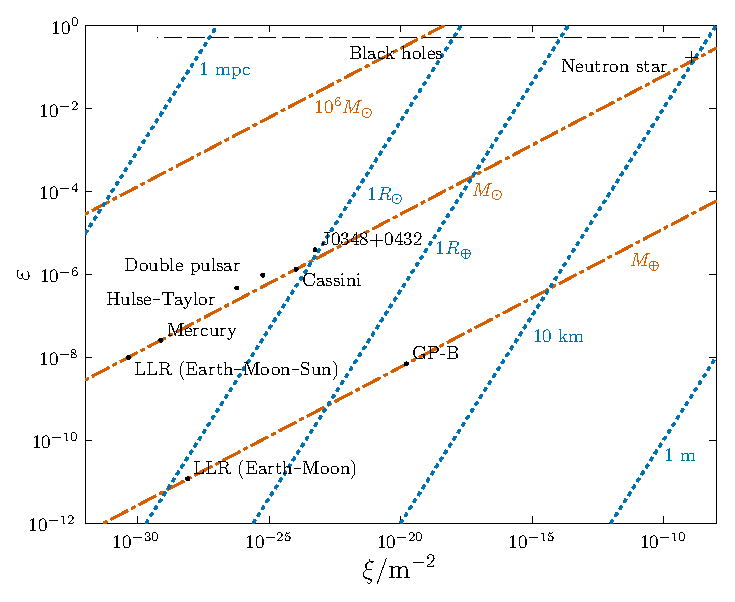
\includegraphics[width=0.6\textwidth]{./images/Fig_Psaltis_plot}
    \caption{Astrophysical tests of GR parameterized by the compactness and curvature scales they probe, adapted from \citet{Psaltis2008a}. The dashed line indicates the Schwarzschild radius $r\sub{S} = 2 r\sub{g}$ for BHs of mass $5$--$10^7M_\odot$ and the cross indicates the surface of an NS.}   
    \label{fig:Psaltis} 
\end{figure}
Included are:
\begin{itemize}
\item The classic perihelion precession of Mercury (\citealt[section 10.2]{Hobson2006}; \citealt[section 7.3]{Will1993}; \citealt{Pitjeva2013});
\item Doppler tracking of the Cassini--Huygens spacecraft \citep{Bertotti2003} which measures the time delay of light travelling passed the Sun \citep[section 7.2]{Will1993};
\item Lunar laser ranging (LLR; \citealt{Bender1973,Williams2012}) which provides precise measurements of the orbits of the Earth--Moon and Earth--Moon--Sun systems \citep[section 8.1]{Will1993};
\item Gravity Probe B (GP-B; \citealt{Everitt2009,Everitt2011}) which produced measurements of the geodetic drift and frame-dragging \citep[section 9.1]{Will1993};
\item A selection of binary pulsars \citep{Taylor1993,Stairs2003}, specifically the Hulse--Taylor binary (PSR B1913$+$16; \citealt{Hulse1975,Weisberg2010}), which was the first discovered and the first system to show the influence of GWs; PSR J0348$+$0432 \citep{Antoniadis2013} which includes a $2 M_\odot$ pulsar, and the double pulsar system (PSR J0737$-$3039;\citep{Breton2008,Kramer2008}. % PSR B1534+12 \citep{Stairs2002};
\end{itemize}
For comparison, we have also plotted the parameters for the surface of an NS and the Schwarzschild radius of BHs of various masses. BHs range in mass from a few solar masses \citep{Ozel2010} to several billion solar masses \citep{Hlavacek-Larrondo2012}, although, for clarity, we have only plotted up to $10^7 M_\odot$. To probe the strongest fields, we need a way of probing the spacetime of compact objects (COs) like NSs and BHs.

In addition to the astrophysical tests of gravity, it is possible to make precision tests in the laboratory \citep{Kapner2007a,Adelberger2009,Wagner2012}. Whilst these are limited to using small masses, they do allow careful control of the system that is not possible in astronomy. Neither the astrophysical nor the laboratory tests performed so far show any discrepancy from the predictions of GR \citep{Will2006}. 

\subsection{Gravitational radiation}

One particularly promising method of exploring strong-field regions would be to observe GWs. These are predicted in any relativistic theory of gravity, where changes in the gravitational field must propagate at finite speed \citep{Schutz1984}. Within GR they are tiny ripples in the spacetime metric (\citealt[section 35.1]{Misner1973}; \citealt[section 107]{Landau1975}). They are generated by systems with a time-varying mass quadrupole; significant gravitational radiation originates from regions where spacetime is highly dynamic and the objects are extremely relativistic. This is precisely the strong-field domain we are interested in investigating.

Some intuition about GWs can be obtained from the more familiar EM waves (\citealt[sections 46--48, 66--67]{Landau1975}; \citealt[sections 7.1, 9.1--9.3]{Jackson1999}). These are oscillations of the electric and magnetic fields produced by accelerating charges whilst GWs are oscillations of the spacetime metric produced by accelerating masses. EM waves may be sourced by a time-varying charge dipole; as a consequence of conservation of momentum there is no time-varying mass dipole, so GWs are sourced by the mass quadrupole (\citealt[section 18.5]{Hobson2006}; \citealt[section 15.4]{Rindler2006}). Both waves propagate at the speed of light and have two (transverse) polarizations: for GWs these represent two orthogonal patterns of stretching and squeezing as shown in \figref{plus-cross} (\citealt[section 34]{Dirac1996}; \citealt[section 18.4]{Hobson2006})
\begin{figure}
  \centering
  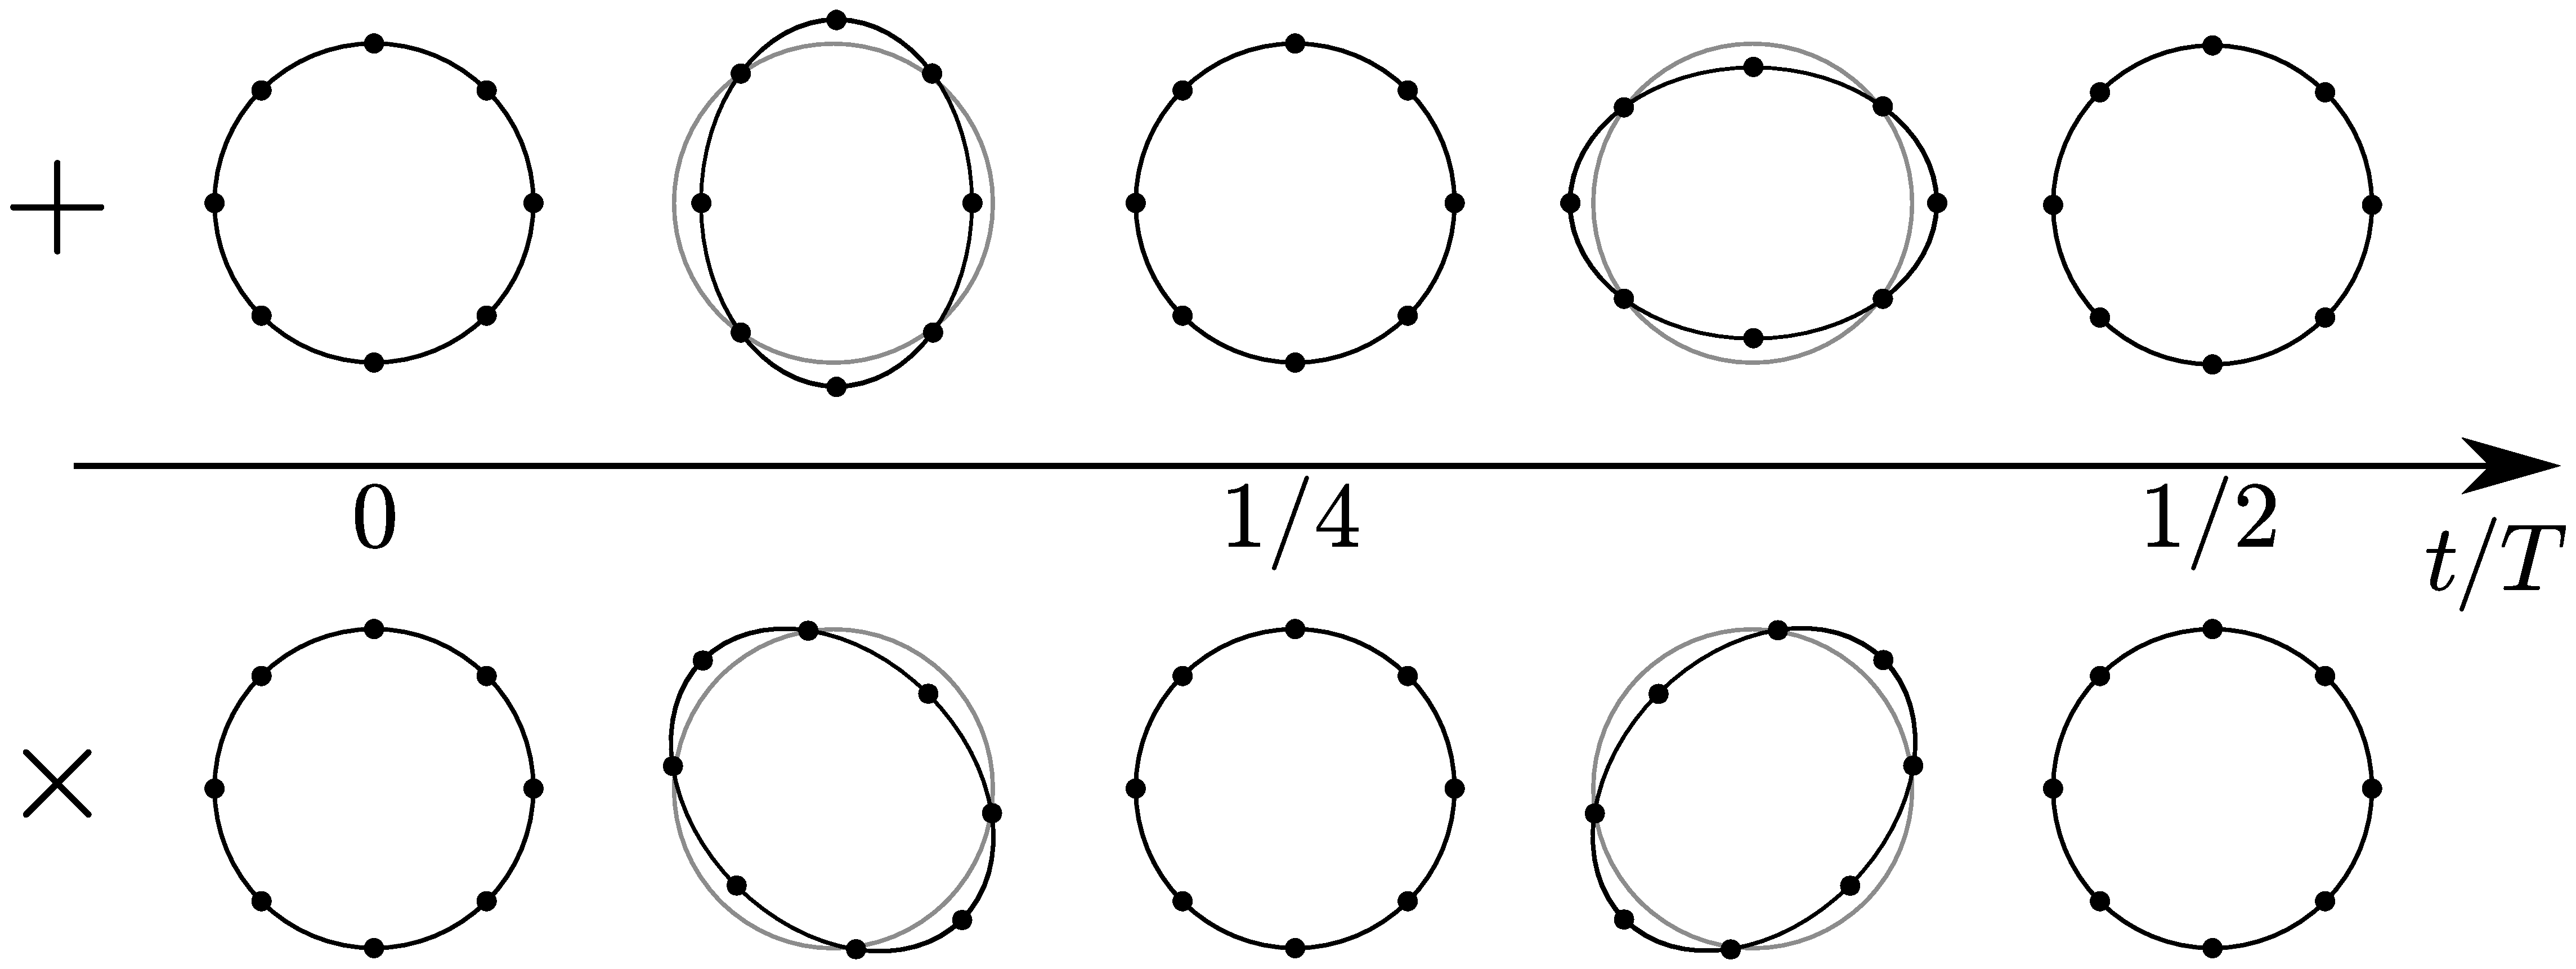
\includegraphics[width=0.7\textwidth]{./images/Polarization}
    \caption{The effect of the two GW polarizations (plus $+$ and cross $\times$) on a ring of free particles as a function of time. The propagation direction is perpendicular to the ring. The wave period is $T$.}   
    \label{fig:plus-cross} 
\end{figure}

Visible light has been used by astronomers for millennia. In the twentieth century, the useful spectrum was extended through infrared to radio, and from ultraviolet to X-rays and gamma rays \citep[chapter 7]{Longair2006}. In the twenty-first century, we hope to move from EM to gravitational radiation. GWs encode valuable information about their sources, information that is accessible by other means.

Just like EM waves, GWs come in a range of frequencies. The frequency is set by the scale of the source system: typically more massive objects have longer associated time-scales and so produce lower frequency radiation. \Figref{spectrum} shows the GW spectrum with illustrative detectors and sources.
\begin{figure}
  \centering
  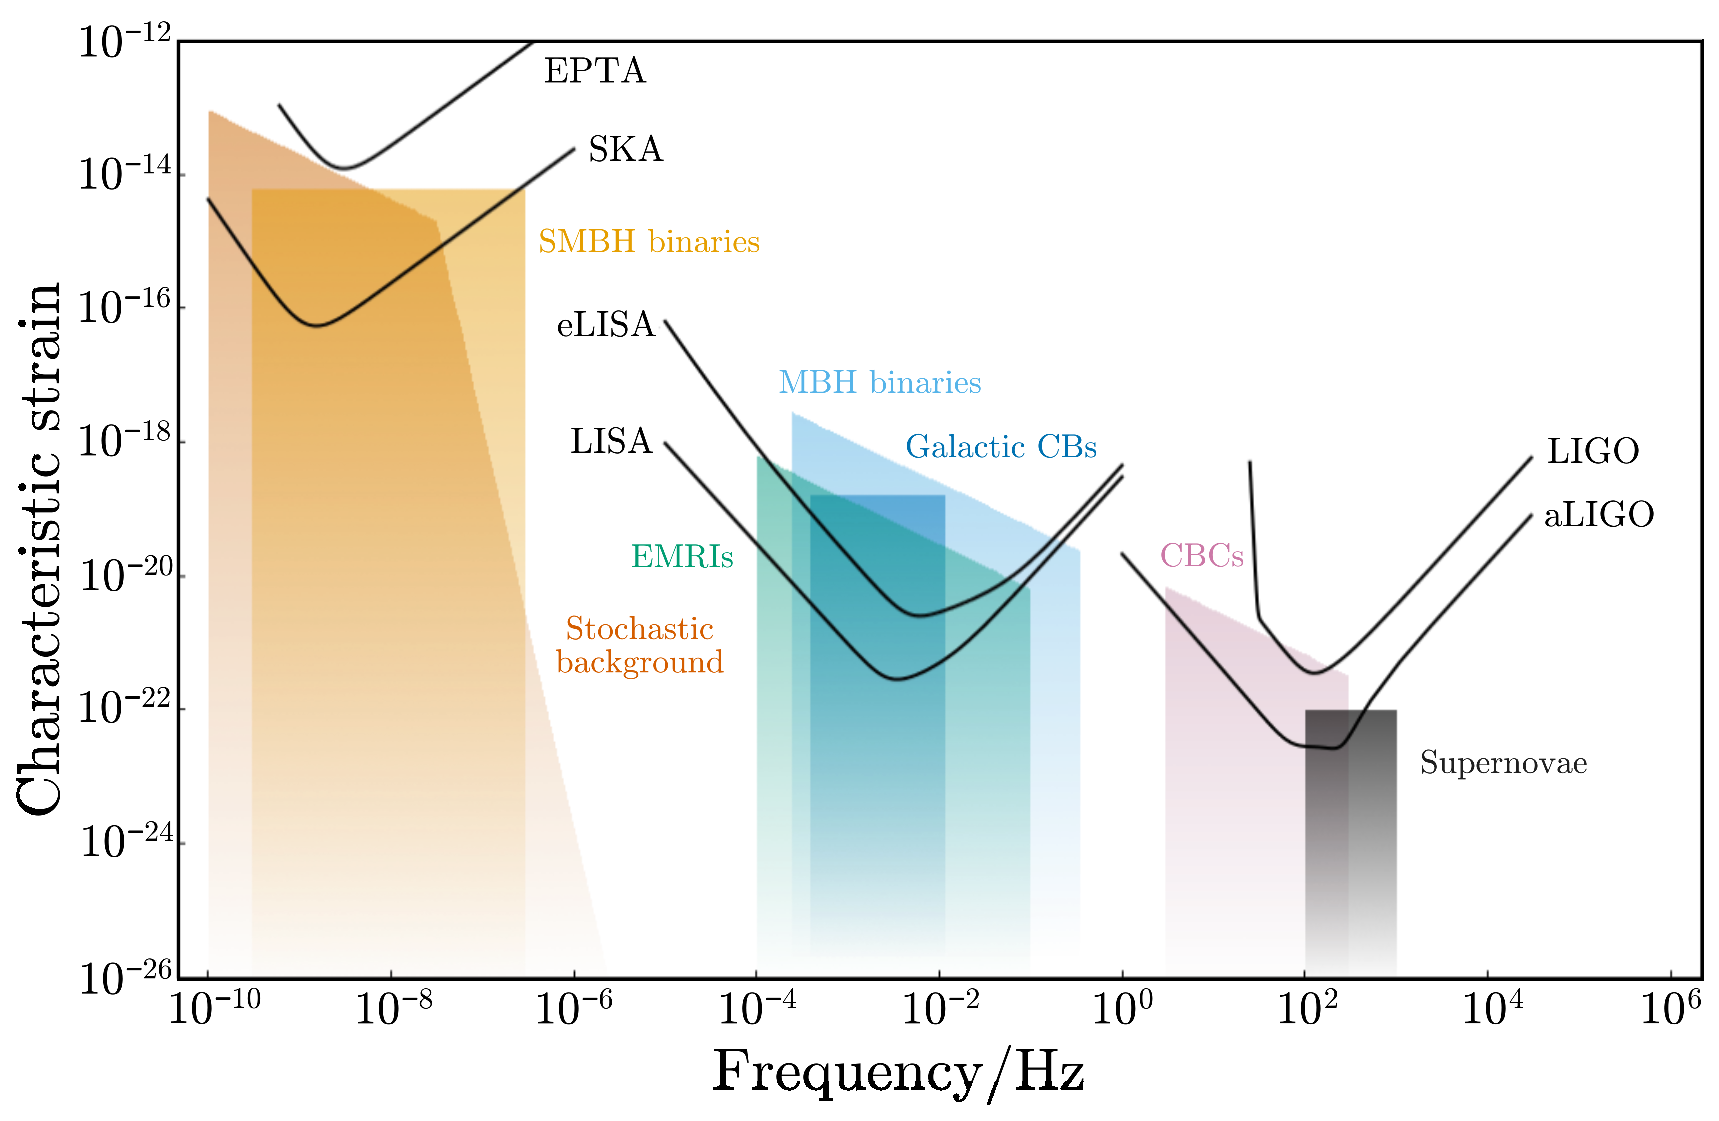
\includegraphics[width=0.675\textwidth]{./images/GW_spectrum}
    \caption{Cartoon spectrum of GWs. Sources (see \secref{GW-sources}) are indicated by their characteristic amplitude as measured on Earth, detectors (see \secref{GW-det}) are characterised by their sensitivity curves. Adapted from \url{http://www.ast.cam.ac.uk/~rhc26/sources/}.}   
    \label{fig:spectrum} 
\end{figure}
Detectors are sensitive to specific frequency bands, the range of which is set by their size. The spectrum may be divided into: the extremely low frequency (ELF; not shown in the figure) regime, $\sim10^{-18}$--$10^{-15}\units{Hz}$, which may be indirectly detected through observations of the polarization of the CMB \citep[e.g.,][]{Hu1997,Kamionkowski1997}; the very low frequency (VLF) regime, $\sim10^{-9}$--$10^{-6}\units{Hz}$, which is accessible to pulsar timing arrays (PTAs); the low frequency (LF) regime, $\sim10^{-6}$--$1\units{Hz}$, which could be measured by space-borne detectors, and the high frequency (HF) regime, $\sim1$--$10^4\units{Hz}$, which is the target range for ground-based detectors. Individual detectors are discussed in \secref{GW-det} and some example sources are introduced in \secref{GW-sources}.

While GWs are an exciting source of information, it will be beneficial to compare with results from other techniques, to maximise the data available for inferences, and to check models. For example, very long baseline interferometry (VLBI) may be used to image the vicinity of a BH's horizon, or X-ray observations could be used to investigate BH accretion discs \citep{Psaltis2008}.

\subsubsection{Gravitational wave detection}\label{sec:GW-det}

As yet no GWs have been directly detected, although their existence has been inferred from the loss of energy and angular momentum from binary pulsars \citep{Stairs2003}. ... There are a number of experiments designed to directly observe GWs \citep{Riles2012}. Modern detectors attempt to measure the minute changes in distance induced by a passing GW (\citealt[section 9.5]{Thorne1987}; \citealt[section 18.9]{Hobson2006}). The amplitude of a GW is characterised by a strain: the fractional change in length resulting from the perturbation from the background spacetime.

The Laser Interferometer Gravitational-wave Observatory (LIGO; \citealt{Abramovici1992}) and the European Gravitational Observatory's Virgo detector \citep{Acernese2008a}, which work in collaboration, are currently being upgraded to their advanced configurations (aLIGO and aVirgo) and are expected to make the first detection shortly after recommencing operation around 2015 \citep{Harry2010,Accadia2011}.\footnote{An optimistic hope is to celebrate the centenary of Einstein's 1916 prediction of GWs \citep[document 32]{Einstein1997} with the first direct detection.} These are ground-based interferometers that detect passing GWs by measuring the induced difference in the length of their two arms \citep{Pitkin2011}. They are sensitive to frequencies in the range $\sim10$--$10^4\units{Hz}$, with peak sensitivity at about $100\units{Hz}$. The LIGO and Virgo detectors are supported by GEO 600, a smaller interferometric experiment that incorporates prototype technologies \citep{Willke2002,Willke2006}. LIGO has two sites, one in Hanford, Washington and one in Livingstone, Louisiana. The Hanford observatory has two detectors, one half the arm-length of the other. There is an agreement to move the smaller detector to a location in India \citep{Unnikrishnan2013}. The LIGO-India detector, operated by the Indian Initiative in Gravitational Observations (IndIGO), provides a longer baseline between detectors, giving improved sky location and sky coverage \citep{Schutz2011}.

A further ground-based interferometer is under construction in Japan. The Kamioka Gravitational Wave Detector (KAGRA), formerly the Large-scale Cryogenic Gravitational Wave Telescope (LCGT; \citealt{Kuroda1999,Kuroda2010}) will operate underground in the Kamioka mine. It lags several years behind the other detectors, aiming to start observations in 2017--2018, but will employ more sophisticated noise-reduction techniques such as cryogenic cooling \citep{Somiya2012}.

Ground-based GW astronomy may eventually be continued by the construction of the Einstein Telescope, an ambitious idea to construct an underground detector with $10\units{km}$ arms \citep{Punturo2010,Hild2011,Sathyaprakash2012}. Its location would provide shielding from seismic noise, allowing it to observe frequencies $10$--$10^4\units{Hz}$. There is no definite time-line for this concept.

There is another contender for the first detection: PTAs \citep{McWilliams2012,Sesana2012a}. These infer the presence of a GW from periodic delays in the arrival times of the highly regular millisecond pulses. In effect, the pulsars are used to create a detector with galactic-scale arms \citep{Hellings1983}. They are sensitive to frequencies of $\sim10^{-9}$--$10^{-7}\units{Hz}$. An international collaboration of European, North American and Australian radio telescopes is already in possession of the necessary instruments to detect GWs \citep{Hobbs2010}.\footnote{The International Pulsar Timing Array (IPTA) consortium consists of the European Pulsar Timing Array (EPTA), the North American Nanohertz Observatory for Gravitational Waves (NANOGrav) and the Parkes Pulsar Timing Array (PPTA) consortia.} The completion of the Square Kilometre Array (SKA; \citealt{Dewdney2009}) shall augment the search, greatly increasing sensitivity \citep{Kramer2004}.

Between the HF range of the ground-based detectors and the VLF range of PTAs, lies a band that could be accessible to space-based interferometers. These are not limited by seismic noise and are free to have much longer arms than the ground-based detectors, making them sensitive to low frequencies. The paradigm detector is the Laser Interferometer Space Antenna (LISA; \citealt{Bender1998, Danzmann2003}). This is a constellation of three satellites in a circular, heliocentric orbit forming a three-armed interferometer. Each arm is $5 \times 10^9\units{m}$, and the orbit trails $20^{\circ}$ behind the Earth. The detector is sensitive to a range of frequencies $\sim10^{-5}$--$1\units{Hz}$, having peak sensitivity around $10^{-3}$--$10^{-2}\units{Hz}$.

LISA developed as a joint NASA--ESA mission. In 2011 NASA withdrew for financial reasons leaving ESA to investigate reduced cost missions. The resulting descoped concept is the evolved Laser Interferometer Space Antenna (eLISA; \citealt{Jennrich2011, Amaro-Seoane2012a}).\footnote{This was submitted to the ESA for their L1 mission selection as the New Gravitational-wave Observatory (NGO).} This shares the same basic components as LISA but only has two arms and lags $9^{\circ}$ behind the Earth. The arms are $1 \times 10^9\units{m}$; this shifts the peak sensitivity to marginally higher frequencies, around $10^{-2}\units{Hz}$. Overall the noise curve is raised relative to LISA giving eLISA reduced sensitivity.

At the time of writing, there is no currently funded mission. However, LISA Pathfinder, a technology demonstration mission, is due for launch in 2015 \citep{Anza2005, Antonucci2012}. Hopefully, a full mission shall follow in the subsequent decade.\footnote{At the time of writing a science theme has been submitted to ESA for their L2/3 mission selection.}

In addition to the LISA family, there are other proposed space-borne detectors. The Japanese Deci-hertz Interferometer Gravitational Wave Observatory (DECIGO; \citealt{Kawamura2006,Kawamura2011}) consists of constellations of satellites similar to LISA, but with arms of $100\units{km}$. It fills the gap between the LISA family and the ground-based detectors, being most sensitive to frequencies $0.1$--$10\units{Hz}$. DECIGO is imagined for launch in 2027, pending the success of two pathfinder missions \citep{Ando2010}.

There have even been suggestions for successors to LISA \citep{Crowder2005}. The Advanced Laser Interferometer Antenna (ALIA) and the Big Bang Observer (BBO) are both popular concepts. Compared to the LISA family, they have shorter arms, making them sensitive to higher frequencies, and better sensitivities. They may be more comparable to DECIGO \citep{Yagi2011a}. These designs are highly speculative.

\subsubsection{Gravitational wave sources}\label{sec:GW-sources}

GWs can be emitted by a variety of systems. To produce detectable signals the source must consist of extremely massive objects moving at a significant fraction of the speed of light. The quintessential source is a binary. These inspiral as a result of GW emission and eventually merge. There is a wide range of binary systems, examples include:
\begin{itemize}
\item Compact binaries (CBs) made up of two closely-orbiting stellar-mass COs, most commonly white dwarfs (WDs). These are the end result of the stellar evolution of a binary star system \citep{Postnov2006}. Wider CBs in the Galaxy are a source for space-borne detectors. These are so common in that some may form an unresolvable foreground \citep{Nelemans2009}; others would be guaranteed sources allowing us to verify the functionality of the detector \citep{Stroeer2006}. At the end of their inspiral, the system merges in a CB coalescence (CBC). This produces a target signal for ground-based detectors \citep{Abadie2010a} as well as a potential EM counterpart \citep[e.g.,][]{Webbink1984,Iben1984,Metzger2010,Rezzolla2011,Nakar2011}. Observations of CBs will help us to understand stellar evolution, in particular common envelope evolution \citep{Ivanova2013}.

\item MBH binaries consisting of two BHs with masses $\gtrsim 10^5 M_\odot$ \citep{Sesana2013b}; BHs at the upper end of the mass spectrum ($\gtrsim10^8$--$10^9 M_\odot$) are sometimes referred to as supermassive black holes (SMBHs). MBHs are found in the centre of galaxies \citep{Lynden-Bell1969,Ferrarese2005}. When galaxies merge, their MBHs also spiral together \citep{Volonteri2003,Schnittman2013}. The inspiral, merger and subsequent ring-down of the new MBH are all promising sources of GWs \citep{Flanagan1998}. Mergers are potentially the loudest GW signals. The combination of many inspirals should result in a stochastic background observable with PTAs \citep{Sesana2008}.

\item Extreme-mass-ratio (EMR) systems of a stellar-mass CO orbiting an MBH. They evolve slowly as a consequence of their large mass-ratio \citep{Glampedakis2005,Barack2009}. EMR systems with highly eccentric orbits produce a burst of GWs as they pass through periapsis; these are EMRBs and are in frequency range of a LISA-like detector \citep{Rubbo2006}. Near circular orbits, as are expected to form in the last few years of inspiral prior to plunge, emit continuously within LISA's frequency band. These signals are extreme mass-ratio inspirals (EMRIs; \citealt{Amaro-Seoane2007}). EMRIs can be observed over many orbits, allowing exquisitely high signal-to-noise ratios (SNRs) to accumulate. This makes them excellent probes of the background geometry permitting both  precision measurements of the system parameters and tests of GR \citep[e.g.,][]{Babak2010}.
\end{itemize}
In addition to binaries, there are other potential sources of GWs. Supernovae are highly energetic, asymmetric explosions when a giant star ejects its outer envelope as its core collapses to an NS or BH; these generate HF bursts of GWs \citep{Dimmelmeier2002,Kotake2006}. Rotating NSs are a source of continuous HF GWs if they possess some degree on axial asymmetry \citep{Abbott2007,Prix2009}. More speculatively, early Universe processes, such as inflation \citep{Grishchuk2005} or a first-order phase transition \citep{Binetruy2012}, could have created GWs. Cosmic strings have also been hypothesised as a potential source \citep{Damour2005,Binetruy2012}. These relic GWs have been predicted across a range of frequencies and their discovery would be an exciting probe of the Universe before the emission of the CMB. Measuring the properties of GWs can tell us both about their source and the nature of gravity.

\section{Astrophysical compact objects}

To probe regions of strong gravity we need massive COs. These are provided in nature through the remnants of stellar evolution \citep[section 1.1]{Shapiro1983}. Depending upon its mass, a star may end its life as a WD, NS or BH. More massive BHs can be found, having grown through other means.

\subsection{White dwarfs and neutron stars}

The least massive stars ($\sim0.6$--$8M_\odot$) end their lives as WDs \citep{Poelarends2008}. These are made of electron-degenerate matter that form from the stellar cores once their outer envelopes are lost \citep{Althaus2010}. WDs' faint luminosity comes from thermal emission. Eventually they cool, dimming and becoming black dwarfs \citep[section 4.2]{Shapiro1983}; because of the long cooling times, no black dwarfs have yet formed.

WDs have maximum mass set by electron degeneracy pressure. This is known as the Chandrasekhar limit and is around $1.4 M_\odot$ (\citealt[section 3.4]{Shapiro1983}; \citealt{Nomoto1987,Timmes1996}). %\footnote{It is possible for WDs to collapse at lower masses during electron-capture supernovae.}
Above this the WD will collapse under its weight until neutron degeneracy pressure takes over to balance gravity. We then have a remnant NS or, if the mass is too large for neutron degeneracy to support, a BH \citep{Woosley2002,Langer2012}.

NSs form from stars of initial masses $\gtrsim 8$--$12 M_\odot$ \citep{Woosley2002,Poelarends2008,Langer2012}. They are made of nuclear density materials. The behaviour of matter under these extreme conditions is not well understood, leading to a plethora of different equations of state \citep{Lattimer2012}. Probing the strong-field regions around NSs could not only provide a test of our understanding of gravitation, but also elucidate the properties of extremely dense matter \citep[e.g.,][]{Read2009,Ozel2009,Lackey2012}.

The maximum mass of an NS depends upon its equation of state \citep[section 9.3]{Shapiro1983}. Hence there is no definitive theoretical prediction.\footnote{The most famous upper mass is the Tolman--Oppenheimer--Volkoff limit \citep{Tolman1939,Oppenheimer1939}. This model is known to be inadequate as the calculated mass is too small.} The largest current estimate for an NS mass is $2.74 \pm 0.21 M_\odot$ \citep{Freire2008,Ozel2012}. Once the maximum NS mass is exceeded, the gravitational force becomes overwhelming and the material is crushed down to become a BH \citep[section 12.1]{Shapiro1983}. The initial stellar mass required for a star to end its life as a BH is uncertain, but is estimated to be $\gtrsim 25 M_\odot$ \citep{Woosley2002,Tauris2011}.

\subsection{Black holes}

BHs are fascinating objects: beautifully simple but with many complexities in their interactions. \citet{Michell1784} first theorised a BH. This is not the same as the object that we understand today, but a Newtonian analogue: a star so massive that its escape velocity exceeds the speed of light. A general relativistic BH was first described with the much celebrated Schwarzschild solution \citep{Schwarzschild1916}. Discovered shortly after Einstein's publication of his general theory, this was the first exact solution other than flat spacetime. It is the metric for the space surrounding a spherically symmetric distribution of matter. It also describes a non-rotating, uncharged BH. A BH is a region of spacetime where gravity is so intense that there exists an event horizon, beyond which nothing can escape \citep[section 33.1]{Misner1973}. The nature of BHs was not fully comprehended until many years after Schwarzschild published his metric; astrophysicists had to first realise the existence of WDs and NSs before they could accept the concept of completely collapsed objects \citep{Israel1987}.

Following on from Schwarzschild's discovery, came the solution of \citet{Reissner1916} and \citet{Nordstrom1918} for an electrically charged BH . There was then a long hiatus before \citet{Kerr1963} discovered the metric for a rotating BH. The set of BH solutions was completed by the discovery of the Kerr--Newman metric for charged, rotating BHs \citep{Newman1965}. According to the no-hair theorem, any BH should be described completely by just its mass $M_\bullet$, spin and electric charge \citep{Israel1967, Israel1968, Carter1971, Hawking1972, Robinson1975}. We expect the charge of an astrophysical BH to be negligible, hence we only need two parameters to describe the BHs of nature \citep[sections 36, 51]{Chandrasekhar1992}.

Astrophysical BHs are grouped by their mass. We shall discuss three partitions: stellar-mass BHs, intermediate-mass BHs (IMBHs) and MBHs. MBHs are of major interest in this work and we pay them special attention.

The spin parameter $a$ is related to the BH's angular momentum $J$ by
\begin{equation}
J = M_\bullet ac;
\end{equation}
it is often convenient to use the dimensionless spin
\begin{equation}
a_\ast = \dfrac{cJ}{GM_\bullet^2}.
\end{equation}
The spin has a range of possible values $0 \leq |a_\ast| \leq 1$ \cite[section 66]{Chandrasekhar1992}. A spin $a_\ast = 0$ corresponds to non-rotating BH. In general BHs have some angular momentum, and we are mostly concerned with the Kerr solution.

\subsubsection{Stellar-mass black holes}

Stellar-mass BHs are an endpoint of stellar evolution, the product of the collapse of giant stars too massive to form NSs \citep{Postnov2006}. These have masses of order of a solar mass: observations show a distribution of $\sim5$--$10M_\odot$ \citep{Ozel2010,Farr2010}. Much of our understanding of these BHs comes from observations of X-ray binaries where the presence of a BH is illuminated by the accretion of matter from a companion \citep{Shakura1973,Remillard2006}.

\subsubsection{Intermediate mass black holes}

IMBHs bridge the gap between the other two classes. They are less well studied than the others, and lack concrete observational confirmation \citep{Miller2009a}, but have been proposed as a tentative explanation for some ultraluminous X-ray sources \citep{Feng2011}. They potentially represent an intermediate stage in the evolution of MBHs \citep{Graham2013}.

\subsubsection{Massive black holes}

MBHs have masses $\sim10^5$--$10^{10} M_\odot$. Many, if not all, galactic nuclei have harboured an MBH during their evolution \citep{Lynden-Bell1971, Soltan1982, Rees1984}. Observations have shown that there exist well-defined correlations between the MBHs' masses and the properties of their host galaxies, such as: bulge mass \citep{Kormendy1995,Haring2004,Graham2012a}; luminosity \citep{Magorrian1998,Marconi2003,Graham2013}; velocity dispersion \citep{Ferrarese2000,Gebhardt2000,Tremaine2002,Graham2011}; light concentration \citep{Graham2001}, S{\'e}rsic index \citep{Graham2007a,Savorgnan2013}, and, for spiral galaxies, pitch angle \citep{Seigar2008,Berrier2013}. These suggest coeval evolution of the MBH and galaxy \citep{Peng2007, Jahnke2011}, possibly with feedback mechanisms coupling the two \citep{Haiman2004, Volonteri2009}. The MBH and the surrounding spheroidal component share a common history, such that the growth of one can inform us about the growth of the other.
%m Kormandy1995; Magorrian1998; Haring2004; (breaking) Graham2012a; (breaking) Scott2013
%L Magorrian1998; Marconi2003; Graham2007; Gultekin2009; Graham2013; 
%sigma Ferrarese2000; Gebhardt2000; Tremaine2002; Gultekin2009; Graham2011
%C Graham2001
%n Graham2001; Graham2007a; Savorgnan2013
%P Seigar2008; Berrier2013

The best opportunity to study MBHs comes from the compact object in the Galactic centre (GC), which is coincident with Sagittarius A* (Sgr A*). Through careful monitoring of stars orbiting the GC, this has been identified as an MBH of mass $M_\bullet \simeq 4 \times 10^6 M_\odot$ at a distance of only $R_0 \simeq 8\units{kpc}$ \citep{Gillessen2009, Meyer2012}.

The masses of other MBHs have been determined using a selection of techniques. Aside from being inferred from the correlations enumerated above, they can be measured directly using stellar or gas dynamical observations \citep[e.g.,][]{Macchetto1997,vanderMarel1998,Gebhardt2003} or maser measurements of the velocity of a circumnuclear disc \citep[e.g.,][]{Miyoshi1995}. After measuring the masses of MBHs we are left with the question of their spins.

The spin of an MBH is determined by several competing processes. An MBH accumulates mass and angular momentum through accretion \citep{Volonteri2010,King2013}. Accretion from a gaseous disc shall spin up the MBH, potentially leading to high spin values \citep{Volonteri2005}, while a series of randomly orientated accretion events leads to a low spin value: we expect an average value $|a_\ast| \sim 0.1$--$0.3$ \citep{King2006, King2008}. The MBH also grows through mergers \citep{Yu2002, Malbon2007}. Minor mergers with smaller BHs can decrease the spin \citep{Hughes2003, Gammie2004}, while a series of major mergers, between similar mass MBHs, would lead to a likely spin of $|a_\ast| \sim 0.7$ \citep{Gonzalez2007, Berti2007, Berti2008}. Measuring the spin of MBHs shall help us understand the relative importance of these processes, and perhaps shall give a glimpse into their host galaxies' pasts.

Elliptical and spiral galaxies are believed to host MBHs of differing spins because of their different evolutions: we expect MBHs in elliptical galaxies to have on average higher spins than MBHs in spiral galaxies, where random, small accretion episodes have played a more important role \citep{Volonteri2007, Sikora2007}.

It has been suggested that the spin of the Galaxy's MBH could be inferred from careful observation of the orbits of stars within a few milliparsecs of the GC \citep{Merritt2010}, although this is complicated because of perturbations due to other stars, or from observations of quasi-periodic oscillations in the luminosity of flares believed to originate from material orbiting close to the innermost stable orbits \citep{Genzel2003a, Belanger2006, Trippe2007, Hamaus2009, Kato2010}, though there are difficulties in interpreting these results \citep{Psaltis2008a}.

%This latter method, combined with a disc-seismology model, has produced a value of the dimensionless spin of $a_\ast = 0.44 \pm 0.08$. To obtain this result \citet{Kato2010} have combined their observations of Sgr A* with observations of galactic X-ray sources containing solar mass BHs, to find a best-fit unique spin parameter for all BHs. However, it is not clear that all BHs should share the same value of the spin parameter; especially considering that the BHs considered here differ in mass by six orders of magnitude, with none in the intermediate range. Even if BH spin is determined by a universal process, we still expect some distribution of spin parameters \citep{King2008, Berti2008}. Thus we cannot precisely determine the spin of the Galactic Centre's MBH from an average including other BHs.

A further possibility is to use VLBI to resolve features of the size of the order of the event horizon \citep{Doeleman2008,Fish2010}. The Galactic MBH, as a consequence of its mass and proximity, is the prime candidate, subtending about $50\units{\upmu as}$ on the sky \citep{Broderick2009,Johannsen2012a}. With this capability, it would be possible to directly image accretion flows down to the horizon and also observe the MBH's shadow. This is the dark region surrounding the BH from which no light can reach the observer; it is bounded by the innermost photon orbit \citep[section 63]{Chandrasekhar1992}. The position of the horizon and the exact shape of the shadow are determined by the metric. By measuring them it may be possible to measure the spin and inclination of the BH \citep{Hioki2009a}, assuming it is Kerr, check whether it is an over-extreme Kerr BH \citep{Bambi2009}, or even probe deviations from Kerr \citep{Johannsen2010a, Johannsen2010b}.%\footnote{Observing deviations from Kerr would disprove the no-hair theorem (possibly admitting naked singularities); suggest a compact object described by an alternative metric such as a Manko-Novikov solution \citep{Manko1992, Gair2008}; provide evidence for a non-GR theory of gravity, or some combination of these options.}
The shape of the shadow of a Kerr BH is shown in \figref{Shadow}.
\begin{figure}%[htb]
\vspace{0.5\baselineskip}
  \centering
   \subfigure[$a_\ast = -0.2$, $\theta\sub{obs} = \pi/2$]{\resizebox{0.3\textwidth}{!}{\import{./Images/}{Shadow_2-psfrag.tex}}} \quad
   \subfigure[$a_\ast = -0.2$, $\theta\sub{obs} = \pi/6$]{\resizebox{0.3\textwidth}{!}{\import{./Images/}{Shadow_2_6-psfrag.tex}}} \quad
   \subfigure[$a_\ast = 0.4$, $\theta\sub{obs} = \pi/2$]{\resizebox{0.3\textwidth}{!}{\import{./Images/}{Shadow_4-psfrag.tex}}} \\
   \subfigure[$a_\ast = 0.4$, $\theta\sub{obs} = \pi/6$]{\resizebox{0.3\textwidth}{!}{\import{./Images/}{Shadow_4_6-psfrag.tex}}} \quad
   \subfigure[$a_\ast = 0.9$, $\theta\sub{obs} = \pi/2$]{\resizebox{0.3\textwidth}{!}{\import{./Images/}{Shadow_9-psfrag.tex}}} \quad
   \subfigure[$a_\ast = 0.9$, $\theta\sub{obs} = \pi/6$]{\resizebox{0.3\textwidth}{!}{\import{./Images/}{Shadow_9_6-psfrag.tex}}} \\
   \subfigure[$a_\ast = 0.998$, $\theta\sub{obs} = \pi/2$]{\resizebox{0.3\textwidth}{!}{\import{./Images/}{Shadow_998-psfrag.tex}}} \quad  
   \subfigure[$a_\ast = 0.998$, $\theta\sub{obs} = \pi/6$]{\resizebox{0.3\textwidth}{!}{\import{./Images/}{Shadow_998_6-psfrag.tex}}}
    \caption{Apparent shape of a Kerr BH shadow viewed from infinity, $\alpha$ and $\beta$ are the position coordinates projected onto the sky, and $\theta\sub{obs}$ is the polar coordinate of the observer \citep[section 63]{Chandrasekhar1992}. The shadow is circular when viewed along the spin axis ($\theta\sub{obs} = 0, \pi$).} 
    \label{fig:Shadow}
\end{figure}
The shadow remains near circular for spin values $|a_\ast| \lesssim 0.9$ regardless of inclination even though the Kerr spacetime is highly non-spherically symmetric \citep{Johannsen2010b}. Weak constraints already exist from VLBI observations \citep{Broderick2009a,Broderick2011}; these determine that the spin is likely not high: $|a_\ast| = 0$--$0.64$ at $68\%$ confidence and $|a_\ast| = 0$--$0.86$ at $95\%$ confidence. Determining the spin to high precision is difficult. 

The spins of MBHs in active galactic nuclei have been inferred using X-ray observations of $\mathrm{Fe}$ $\mathrm{K}$ emission lines \citep{Miller2007, McClintock2011}. So far this has been done for a handful of other galaxies' MBHs, as shown in \tabref{X-ray}.
\begin{table}\footnotesize
\centering
\begin{tabular}{l D{,}{.}{3.11} l }
\toprule
\multicolumn{1}{c}{AGN} & \multicolumn{1}{c}{$a_\ast$} & \multicolumn{1}{c}{Study} \\ \midrule 
1H 0323$+$342 & >0,37 & \citet{Walton2013} \\ % 90%
1H 0419$-$577 & >0,89 & \citet{Walton2013} \\ % 90%
1H 0707$-$495 & \geq 0,976 & \citet{Zoghbi2010} \\ % 90%
3C 120 & 0,994^{+0.002}_{-0.003} & \citet{Lohfink2013} \\
3C 382	& <0,81 & \citet{Walton2013} \\ % 90%
%Ark 120 & $<0.94$ & \citet{Patrick2011} \\ % 90%
Ark 120 & 0,74^{+0.19}_{-0.50}{^\dagger} & \citet{Nardini2011} \\ % 99% confidence
 & 0,64^{+0.19}_{-0.11} & \citet{Walton2013} \\ % 90%
Ark 564 & 0,96^{+0.01}_{-0.07} & \citet{Walton2013} \\ % 90%
Fairall 9 & 0,60 \pm 0.07{^\ast} & \citet{Schmoll2009} \\ % 68%
 & 0,44^{+0.04}_{-0.11} & \citet{Patrick2011} \\ % 90%
 & 0,39^{+0.48}_{-0.30} & \citet{Emmanoulopoulos2011} \\ % 90%
 & 0,67^{+0.10}_{-0.11} & \citet{Patrick2011a} \\ % 90%
 & 0,52^{+0.19}_{-0.15} & \citet{Lohfink2012} \\ % 90%
 & 0,82^{+0.09}_{-0.19} & \citet{Walton2013} \\ % 90% 
IRAS 00521$-$7054 & 0,97^{+0.03}_{-0.13} & \citet{Tan2012} \\ % 90%
IRAS 13224$-$3809 & 0,988 \pm 0.001{^\ast} & \citet{Fabian2013} \\ % 68%
%MGC$-$02-14-009 & $<0.88$ & \citet{Patrick2011} \\ % 90%
MCG$-$6-30-15 & 0,989^{+0.009}_{-0.002} & \citet{Brenneman2006} \\ % 90%
 & 0,86^{+0.01}_{-0.02} & \citet{delaCallePerez2010} \\ % 90%
 & 0,49^{+0.20}_{-0.12} & \citet{Patrick2011a} \\ % 90%
Mrk 79 & 0,7 \pm 0.1 & \citet{Gallo2011} \\ % 90%
Mrk 110 & 0,96^{+0.03}_{-0.07} & \citet{Walton2013} \\ % 90%
Mrk 335 & 0,70^{+0.12}_{-0.01} & \citet{Patrick2011} \\ % 90%
 & 0,83^{+0.09}_{-0.13} & \citet{Walton2013} \\ % 90%
Mrk 359 & 0,66^{+0.30}_{-0.54} & \citet{Walton2013} \\ % 90%
Mrk 509 & 0,78^{+0.03}_{-0.04} & \citet{delaCallePerez2010} \\ % 90%
 & 0,36^{+0.20}_{-0.37} & \citet{Walton2013} \\ % 90%
Mrk 841 & >0,52 & \citet{Walton2013} \\ % 90%
Mrk 1018 & 0,58^{+0.36}_{-0.54} & \citet{Walton2013} \\ % 90%
NGC 1365 & \geq 0,84 & \citet{Risaliti2013} \\ % 90%
NGC 3783 & \geq 0,88{^\dagger} & \citet{Brenneman2011} \\ % 99%
 & < 0,32 & \citet{Patrick2011a} \\ % 90%
NGC 4051 & < 0,94 & \citet{Patrick2011a} \\ % 90%
NGC 7469 & 0,69^{+0.09}_{-0.09} & \citet{Patrick2011} \\ % 90%
 & 0,64^{+0.13}_{-0.20} & \citet{Walton2013} \\ % 90%
%RBS 1125 & $\geq 0.60$ & \citet{Minniutti2010} \\ % Determined from soft excess smoothness which requires a high degree of relativistic blurring, rather than the relativistic iron line shape.
PDS 456 & >0,96 & \citet{Walton2013} \\ % 90%
PKS 0558--504 & >0,95 & \citet{Walton2013} \\ % 90%
RBS 1124 & >0,97 & \citet{Walton2013} \\ % 90%
SWIFT J0501.9$-$3239 & >0,99 & \citet{Walton2013} \\ % 90%
SWIFT J2127.4+5654 & 0,6 \pm 0.2 & \citet{Miniutti2009} \\ % 90%
 & 0,70^{+0.10}_{-0.14} & \citet{Patrick2011} \\ % 90%
Ton S180 & 0,92^{+0.03}_{-0.11} & \citet{Walton2013} \\ % 90%
UGC 6728 & >0,71 & \citet{Walton2013} \\ % 90%
 \bottomrule
\end{tabular}
\caption{Measurements of MBH spin from iron emission lines. Confidence levels are $90\%$ except where indicated otherwise: an asterisk ($^\ast$) is used for $68\%$ and an obelisk ($^\dagger$) is used for $99\%$. The scatter in results indicates the complexities of modelling the accretion disc.\label{tab:X-ray}}
\vspace{-3pt}
\end{table}
Estimates for the spin cover a range of values up to the maximal value for an extremal Kerr black hole. Typical values are in the intermediate range of $a_\ast \sim 0.7$ and above with an uncertainty of about $10\%$ on each measurement. There may be an observational bias toward high spin values \citep{Brenneman2011}.

%While we can use the spin of other BHs as a prior, to inform us of what we should expect to measure for the spin of the Galaxy's MBH, it is desirable to have an independent observation, a direct measurement.

%An exciting means of inferring information about the MBH is through GWs emitted when compact objects (COs), such as stellar mass BHs, neutron stars (NSs), white dwarfs (WDs) or low mass main sequence (MS) stars, pass close by \citep{Sathyaprakash2009}. A space-borne detector, such as the Laser Interferometer Space Antenna (LISA) or the evolved Laser Interferometer Space Antenna (eLISA), is designed to be able to detect GWs in the frequency range of interest for these encounters \citep{Bender1998, Danzmann2003, Jennrich2011, Amaro-Seoane2012a}. The identification of waves requires a set of accurate waveform templates covering parameter space. Much work has already been done on the waveforms generated when companion objects inspiral towards an MBH \citep{Glampedakis2005, Barack2009}; as they orbit, the GWs carry away energy and angular momentum, causing the orbit to shrink until eventually the object plunges into the MBH. These systems are typically formed following two-body encounters so that the initial orbits are highly eccentric; a burst of radiation is emitted during each periapse passage. These are extreme mass-ratio bursts (EMRBs; \citealt{Rubbo2006}). Assuming that the companion is not scattered from its orbit, and does not plunge straight into the MBH, its orbit evolves, becoming more circular, and it shall begin to continuously emit significant gravitational radiation in the LISA/eLISA frequency range. The resulting signals are extreme mass-ratio inspirals (EMRIs; \citealt{Amaro-Seoane2007}).

\section{Modified gravity}

GR is a remarkably successful theory. It satisfies every weak-field theory experiment we have currently devised \citep{Will2006}. However, there may yet be modifications to be revealed in strong-fields. Whilst we have no definite evidence that GR is not the correct classical theory of gravitation, there remain unanswered questions about gravity: What are the true natures of dark matter and dark energy? How should we formulate a quantizable theory of gravity? What drove inflation in the early Universe \citep{Guth1981,Lyth1999}? Therefore, there is motivation for exploration of alternative theories.

Studying modified gravity can be done in two ways: either studying specific alternative theories of gravity to discover what differences manifest, or looking for more general deviations from GR and then using these to constrain possible alternative theories.

\subsection{Alternative theories of gravity}

There are a plethora of modified gravity theories \citep{Clifton2012}. Perhaps the most infamous is the hypothesis of modified Newtonian dynamics (MOND; \citealt{Famaey2012}). Suggested by \citet{Milgrom1983,Milgrom1983a,Milgrom1983b} to match observations of galaxies, Newtonian dynamics is modified at low accelerations such that
\begin{equation}
\mu\left(\dfrac{a}{a_0}\right)\boldsymbol{a} = \boldsymbol{g}
\end{equation}
where $\boldsymbol{g}$ is the Newtonian gravitational field strength, $\boldsymbol{a}$ is the acceleration, $a_0 \approx 10^{-10}\units{m\,s^{-2}}$ is the new acceleration scale and $\mu$ is an interpolation function with properties $\mu(x) \rightarrow 1$ for $x \gg 1$ and $\mu(x) \rightarrow x$ for $x \ll 1$. There are a variety of relativistic theories that can reproduce this behaviour, including Einstein--\ae{}ther theory and tensor--vector--scalar (TeVeS) theory \citep{Bekenstein2006}. The hypothesis works well for describing galactic-scale systems but struggles to reproduce the cosmological predictions of the cold dark matter paradigm. It may be possible to constrain MOND theories in the low-acceleration regime by using LISA Pathfinder to measure acceleration at the Earth--Sun saddle point \citep{Magueijo2011,Galianni2011}. Most alternative theories, however, reduce to the Newtonian limit.

Alternative theories of gravity can be created by adding new fields or modifying the form of the gravitational action \citep{Gair2012a}.\footnote{Here ``or'' is inclusive. In some cases, a modification of the gravitational action can be recast as introducing a new field \citep[e.g.,][]{Wands1994,Jacobson2010}.} We shall introduce a few to illustrate the range.

Including a scalar field in addition to the metric tensor produces scalar--tensor gravity \citep{Wagoner1970,Nordtvedt1970,Fujii2003}. The best known example is Brans--Dicke gravity; this has a scalar field replace the gravitational constant \citep{Brans1961,Dicke1962}. Deviations from GR can be quantified in terms of the Brans--Dicke coupling parameter $\omega\sub{BD}$, as $\omega\sub{BD} \rightarrow \infty$ observable differences become smaller while in a natural theory we might expect $\omega\sub{BD} \sim \order{1}$. Measurements of light deflection from the Cassini--Huygens mission \citep{Bertotti2003} constrain Brans--Dicke to be close to GR as $\omega\sub{BD} > 4 \times 10^4$ \citep{Will2006}.

Vector--tensor gravity introduces a vector field \citep{Will1972,Nordtvedt1972}. This is typically time-like and in Einstein--\ae{}ther theory is constrained to have unit norm \citep{Jacobson2001,Jacobson2008}. These theories have a preferred reference frame specified by the vector field. Preferred frame effects can be constrained by careful observational measurements \citep[chapter 8]{Will1993}.

%Tensor--tensor or bimetric theories have a second metric.

Scalar--vector--tensor gravities have the gravitational field couple to both vector and scalar fields. It is the natural extension to scalar--tensor and vector--tensor gravity. TeVeS includes a metric tensor, a unit vector field, one dynamical scalar field and one non-dynamical scalar field \citep{Bekenstein2004,Skordis2009}. It has three parameters (one setting a length-scale, the others dimensionless) and a free function that can be tuned to either recover MOND or Newtonian behaviour in the weak-field limit, and become arbitrarily close to GR. Bi-scalar--tensor--vector gravity generalises TeVeS by introducing a second dynamical scalar field in place of the non-dynamical field \citep{Sanders2005}. A separate theory is scalar--tensor--vector gravity which contains a vector field and three scalar fields, one of which replaces the Newtonian constant $G$, in addition to a metric \citep{Moffat2006}. This includes an additional repulsive Yukawa force in the weak-field limit. The added freedom of including extra fields allows fitting of a wide range of phenomena.

In $f(R)$-gravity the Einstein--Hilbert action is generalised by including an arbitrary function of the Ricci scalar \citep{Buchdahl1970, Sotiriou2010, DeFelice2010}. The action may be further generalised by using an action including other contractions of the Riemann tensor, such that it becomes $f(R, R_{\mu\nu}R^{\mu\nu}, R_{\mu\nu\rho\sigma}R^{\mu\nu\rho\sigma})$ \citep{Madsen1989, Farhoudi2006, Nojiri2011}. These higher-order gravities, so-called because the action contains derivatives higher than second-order (as in GR), have a rich selection of phenomenology. The flexibility in defining the form of the arbitrary function allows them to be fitted to a range of observations.

Motivated by gauge theories, Chern--Simons gravity includes a term in the action proportional to the Pontryagin density ${^\ast R} R = (1/2)\epsilon^{\nu\rho\sigma\tau}{R^\lambda}_{\mu\sigma\tau}{R^\mu}_{\lambda\nu\rho}$, where $\epsilon^{\nu\rho\sigma\tau}$ is the Levi-Civita alternating tensor, coupled to a (pseudo-)scalar field \citep{Jackiw2003, Smith2008, Alexander2009a}. This introduces gravitational parity violation and, consequently, this theory includes birefringent GWs, altered precession rates, and the modification of vacuum solutions that are axisymmetric but not spherically symmetric such as Kerr. GW observations could place tight constraints on any Chern--Simons correction \citep{Canizares2012}.

Ho\v{r}ava--Lifshitz gravity \citep{Horava2009, Sotiriou2009c, Blas2010a} sacrifices spacetime covariance in favour of being renormalizable. A preferred foliation of space and time along the lines of the Arnowitt--Deser--Misner formalism is adopted \citep{Arnowitt1962a}, with Lorentz invariance being emergent at large distances. This removes many of the problems regarding time traditionally associated with trying to quantize GR. However, there are outstanding problems in producing a viable theory consistent with observations \citep{Sotiriou2011a}.

\subsection{Deviations from general relativity}

Since there is a plethora of alternative theories, it is challenging to expound the observable consequences of all possibilities. Furthermore, it is possible that the true theory of gravitation is something yet to be conceived. It is therefore useful not only to look for the signatures of particular theories, but also to find generic tests that can be used to detect deviations from GR. If these deviations are not observed, we can be more confident in GR and place tighter constraints on viable alternatives, whilst if a deviation is discovered we can select suitable alternatives.

The parameterized post-Newtonian (PPN) formalism provides a simple means of characterising gravity in the weak-field limit \citep[chapter 4]{Will1993}. The PPN framework describes deviations from Newtonian gravity. There are ten parameters: $\gamma$ which quantifies the space-curvature produced by a mass; $\beta$ which quantifies the non-linearity in the superposition law; $\xi$ which measures preferred-location effects; $\alpha_1$--$\alpha_3$ which quantify any preferred-frame effects, and $\zeta_1$--$\zeta_4$ (with $\alpha_3$) which measure non-conservation of momentum. These can differ in GR and alternative theories. Current PPN limits are imposed using a variety of tests, such as those included in \secref{exist-tests} \citep{Will2006}. The soon-to-be-launched Gaia mission, which provides high-precision astrometry measurements, shall give improved measurements of $\gamma$ and $\beta$ through careful monitoring of light-bending and the motion of asteroids \citep{Mignard2010, Hobbs2010a, Hestroffer2010}. Whilst PPN are useful in the weak-field, we wish to find strong-field equivalents.

The ideal probe of strong-field gravity is gravitational radiation. GWs can be modified in alternative theories of gravity. One modification is the addition of other polarizations. There may be up to six polarizations in a general metric theory (\citealt{Eardley1973}; \citealt[section 10.2]{Will1993}): as well as the two standard tensor modes, $h_+$ and $h_\times$, there can be two scalar modes (longitudinal and transverse) and two vector modes (assuming a wave propagating in the $z$-direction, one mode oscillates in the $x$--$z$ plane and another in the $y$--$z$ plane). These other polarizations are observable with GW detectors \citep{Tinto2010,Alves2011,Blaut2012}; their discovery would be decisive evidence against GR.

Restricting ourselves to the standard two polarizations, modifications to the gravitational waveform can be described in terms of the parameterized post-Einsteinian (PPE) framework \citep{Yunes2009a}. This follows in the footsteps of the PPN formalism by providing a set of parameters that can be adjusted to fit different theories. Constraining these can place limits on deviations from GR or select viable alternative theories \citep{Cornish2011}. The post-Einsteinian parameters were developed to describe the quasi-circular inspiral, merger and ring-down of binary non-spinning BH-like objects. Although designed for measuring anomalies in GWs, it is possible to impose some bounds on the plausible range of post-Einsteinian parameters using observations of binary pulsars \citep{Yunes2010}.

Measuring the propagation speed of GWs is another test of relativistic gravity \citep[section 10.1]{Will1993}. Any deviation from $c$ would be evidence for an alternative theory. This can happen in theories with massive gravitons \citep{Babak2003,Goldhaber2010}. In this event, GWs also become dispersive. If there are additional polarization modes, these can travel at different speeds. The GW speed can be measured by comparing arrival times for EM counterparts \citep[e.g.,][]{Cooray2004,Kocsis2008} or by monitoring the phase evolution of an inspiral \citep{Will1998,Berti2011}.

In addition to scrutinizing the gravitational radiation itself, we can use it to study its source. The BHs of GR are Kerr solutions and so specified entirely by their mass and spin. The mass multipole $M_\ell$ ($M_0 \equiv M_\bullet$) and mass-current multipole moments $S_\ell$ ($S_1 \equiv J/c$) are determined from these according to \citep{Hansen1974}
\begin{equation}
M_\ell + iS_\ell = M_\bullet \left(ia\right)^\ell.
\end{equation}
Checking this consistency relation for higher multipoles is a method of testing whether a CO is a Kerr BH as expected \citep{Gair2012}. For example, in Chern--Simmons gravity, the BH solution differs at the fourth multipole \citep{Sopuerta2009a}.  The structure of the spacetime about an object is determined by these multipole moments \citep{Geroch1970}. EMRI observations can be used to build a detailed map of the spacetime of a massive CO. Information regarding the multipole moments is encoded within the frequency spectrum of the GWs \citep{Ryan1995,Ryan1997}.

Introducing higher-order multipole moments results in the creation of a bumpy BH. These have been studied to discover the observable consequences of deviations from Kerr. A variety of different bumpy metrics have been considered; these include stationary and axisymmetric deformations of Schwarzschild which are solutions of the Einstein equations \citep{Collins2004} and, similarly, deformations of Kerr \citep{Vigeland2010a}; a quasi-Kerr metric with an arbitrary mass quadrupole \citep{Glampedakis2006a,Barack2007}; the metric of \citet{Manko1992}, which is a solution of Einstein's equations with arbitrary higher-order mass multipole moments \citep{Gair2008}; perturbed Kerr metrics that are not required to satisfy the Einstein equations but do preserve an approximate Carter-like constant \citep{Vigeland2011,Gair2011}, and an axisymmetric Kerr-like metric, where the perturbations are different powers of $M_\bullet/r$, which is required neither to be a solution of the Einstein equations nor have full integrability of its geodesic motion \citep{Johannsen2011}. All these metrics deviate from the standard Kerr solution by a small amount and reduce down to it as the perturbation goes to zero; if the perturbation is large enough it can be detected with EMRIs.

%%The majority of the work to date has focused on spacetimes that are solutions in GR, but which deviate from the Kerr solution. However, if GR was not the correct theory of gravity, this could also lead to detectable signatures in the observed gravitational waves. Certain alternative theories of gravity, including $f(R)$, do admit the Kerr metric as a solution, since it has vanishing Ricci tensor, $R_{\mu\nu} = 0$~\cite{Psaltis2008, Yunes2011}. However, the Kerr metric need not be the expected end state of gravitational collapse~\cite{Barausse2008}. If a Kerr BH existed in an alternative theory, the geodesics would be the same, but the energy flux carried by the GWs could still be different, and so differences would show up in the rate of inspiral; although in many cases these differences do not appear at leading order. In most cases, however, either the Kerr metric is not admitted as a solution, or it is not the correct metric to describe collapsed objects~\cite{Yunes2011}. Waveform differences then show up as a result of the differences in the instantaneously-geodesic orbits of the compact object involved in the EMRI. Since the leading-order energy-momentum tensor of the GWs often takes the same form as in GR~\cite{Stein2011}, this is the primary effect and means the problem of testing alternative theories through EMRI observations is equivalent to the spacetime mapping programme within GR described previously.

%There are also certain qualitative features that could be smoking-guns for a departure from the Kerr metric, such as ergodicity in the orbits~\citep{Gair2008}, persistent resonances~\citep{Lukes-Gerakopoulos2010} or a shift in the frequency of plunge~\citep{Kesden2005, Gair2008}.

%%As a consequence of the difficulties of solving for GW emission in alternative theories, work on testing alternative theories of gravity using LISA EMRIs has so far been restricted to a few cases. In Brans-Dicke gravity, in which the gravitational field is coupled to a scalar field, differences show up due to a modification to the inspiral rate that arises from dipole radiation of the scalar field~\cite{Berti2005}. Neutron star EMRIs are required since the dipole radiation depends on a sensitivity difference between the two objects, and the sensitivity is the same for all BHs. Lower mass central BHs provide the most powerful constraints, but a LISA observation of a neutron star EMRI into a $10^4 M_{\odot}$ BH could place constraints on the Brans-Dicke coupling parameter that are competitive with Solar System constraints~\cite{Berti2005}. In dynamical Chern-Simons modified gravity, the action is modified by a parity-violating correction, inspired by string theory~\cite{Alexander2008, Alexander2009a}. In this case, the BH solution differs from the Kerr solution at the fourth multipole, $l = 4$, but the energy-momentum tensor of gravitational radiation takes the same form as in GR~\cite{Sopuerta2009a}. LISA observations of EMRIs should place constraints on the Chern-Simons coupling parameter that are an order of magnitude better than will be possible from binary pulsar observations, although a full analysis accounting for parameter degeneracies has not yet been carried out~\cite{Sopuerta2009a}. 

\section{Overview}

Developments in our theoretical understanding of gravity are driven by astronomical observations. Astrophysical systems are dominated by gravitational interactions, our understanding of them can be enhanced by using gravitational probes. To date, gravity has only been studied in the weak-field regime. Exploring the strong-field regime, as found around COs such as BHs, shall deliver new insights. We could learn about the evolution of MBHs, and by implication their surrounding galaxies, or uncover modifications to GR. One promising means of delving into the strong-field, is through GW astronomy. This is in its infancy; what it shall teach us is yet to be revealed, but there is scope for exciting discovery.

We shall study what we learn from strong-field tests and GWs. In \partref{astro} we use GWs, specifically EMRBs, to learn about MBHs. In \partref{grav} we investigate the observable signatures of metric $f(R)$-gravity.


\part{Astronomical systems}\label{pt:astro}

\chapter{Extreme-mass-ratio burst waveforms}\label{ch:waveforms}

\section{Massive black holes and extreme-mass-ratio events}

An exciting means of inferring information about MBHs is through GWs emitted when COs, such as stellar-mass BHs, NSs, WDs or low mass main sequence (MS) stars, pass close by \citep{Sathyaprakash2009}. A space-borne detector, such as LISA, is designed to be able to detect GWs in the frequency range of interest for these encounters \citep{Danzmann2003, Jennrich2011, Amaro-Seoane2012a}. The identification of waves requires a set of accurate waveform templates covering parameter space. Much work has already been done on the waveforms generated when companion objects inspiral towards an MBH \citep{Glampedakis2005, Barack2009}; as they orbit, the GWs carry away energy and angular momentum, causing the orbit to shrink until eventually the object plunges into the MBH. These systems are typically formed following two-body encounters so that the initial orbits are highly eccentric; a burst of radiation is emitted during each periapse passage. These are extreme mass-ratio bursts (EMRBs; \citealt{Rubbo2006}). Assuming that the companion is not scattered from its orbit, and does not plunge straight into the MBH, its orbit evolves, becoming more circular, and it shall begin to continuously emit significant gravitational radiation in the frequency range of a LISA-like space-borne detector. The resulting signals are extreme mass-ratio inspirals (EMRIs; \citealt{Amaro-Seoane2007}).

Studies of these systems have usually focused upon the phase when the orbit is close to plunge and completes a large number of cycles in the detector's frequency band, allowing a high signal-to-noise ratio (SNR) to be accumulated. Here, we investigate high eccentricity orbits. These are the initial bursting orbits from which an EMRI may evolve, and are the consequence of scattering from two-body encounters. The event rate for the detection of such EMRBs with LISA has been estimated to be as high as $15\units{yr^{-1}}$ \citep{Rubbo2006}, although this has been subsequently revised downwards to the order of $1\units{yr^{-1}}$ \citep{Hopman2007}. The event rate is dominated by bursts from the Galactic Centre (GC). Even if only a single burst is detected during a mission, this is still an exciting possibility since the information carried by the GW should give an unparalleled probe of the structure of spacetime of the GC.

To model bursts we make the simplifying assumption that all these orbits are marginally bound, or parabolic, since highly eccentric orbits appear almost indistinguishable from an appropriate parabolic orbit. Here ``parabolic'' and ``eccentricity'' refer to the energy of the geodesic and not to the geometric shape of the orbit.\footnote{Marginally bound Keplerian orbits (in flat spacetime) are parabolic in both senses.} Following such a trajectory an object may make just one pass of the MBH or, if the periapsis distance is small enough, it may complete a number of rotations. Such an orbit is referred to as zoom--whirl \citep{Glampedakis2002a}.

We begin our investigation of the properties of EMRBs as a means of studying MBHs by constructing approximate waveforms. To do so we integrate the geodesic equations for a parabolic orbit in Kerr spacetime (\secref{Geodesic}); we assume that the orbiting body is a test particle, such that it does not influence the underlying spacetime, and that the orbital parameters evolve negligibly during the orbit such that they may be held constant.\footnote{In \apref{evolve} it is shown that orbital evolution is typically negligible for extreme-mass-ratio systems.} We use this trajectory to construct an approximate numerical kludge (NK) waveform \citep{Babak2007} as explained in \secref{Kludge}. In \secref{Signal} we establish what the LISA detectors would measure and how the signal would be analysed. Since there does not exist a definite mission design, we use the classic LISA design for the majority of this work. It is hoped that any future missions shall have comparable sensitivity, and studies using the LISA design are sensible benchmarks for comparison. In a few places we look at the detectability of bursts using eLISA. We confirm the accuracy of the kludge waveforms in \secref{Energy} by comparing the energy flux to fluxes calculated using other approaches. The typical error introduced by the NK approximation may be a few percent, but this worsens as the periapsis approaches the last non-plunging orbit.

Having established the accuracy of our NK waveforms, we study what information can be extracted from them. Exactly what can be inferred depends upon the orbit. We begin in \chapref{param} by looking at EMRBs from the GC as the Galaxy's MBH is the most promising to study. Finding promising results, we extend our study to extragalactic sources in \chapref{extragal}. We complete our analysis of EMRBs in \chapref{events}, where we build a simple model for burst event rates and use this to estimate what we could expect to learn from them.

\section{Parabolic orbits in Kerr spacetime}\label{sec:Geodesic}

\subsection{The metric and geodesic equations}

Astrophysical BHs are described by the Kerr metric \citep{Kerr1963}. In standard Boyer--Lindquist coordinates the line element is (\citealt{Boyer1967}; \citealt[section 13.7]{Hobson2006})
\begin{equation}
\dd s^2 = \dfrac{\varrho^2 \Delta}{\Sigma^2}c^2\dd t^2 - \dfrac{\Sigma \sin^2 \theta}{\varrho^2}\left(\dd \phi - \omega \dd t\right)^2 - \dfrac{\varrho^2}{\Delta}\dd r^2 - \varrho^2\dd \theta^2,
\end{equation}
where we have introduced functions
\begin{subequations}
\begin{align}
\varrho^2 = {} & r^2 + a^2\cos^2\theta,\\
\Delta = {} & r^2 - \dfrac{2GM_\bullet r}{c^2} + a^2,\\
\Sigma = {} & \left(r^2 +a^2\right)^2 - a^2\Delta\sin^2\theta,\\
\omega = {} & \dfrac{2GM_\bullet ar}{c\Sigma}.
\end{align}
\end{subequations}
For the remainder of this section we use natural units with $G = c = 1$.

Geodesics are parameterized by three conserved quantities (aside from the particle's mass $\mu$): energy (per unit mass) $E$, specific angular momentum about the symmetry axis (the $z$-axis) $L_z$, and Carter constant $Q$ (\citealt{Carter1968}; \citealt[section 62]{Chandrasekhar1992}). The geodesic equations are
\begin{subequations}
\begin{align}
\varrho^2 \diff{t}{\tau} = {} & a\left(L_z - aE\sin^2 \theta\right) + \dfrac{r^2 + a^2}{\Delta}T,\\
\varrho^2 \diff{r}{\tau} = {} & \pm \sqrt{V_r},\\
\varrho^2 \diff{\theta}{\tau} = {} & \pm \sqrt{V_\theta},\\
\varrho^2 \diff{\phi}{\tau} = {} & \dfrac{L_z}{\sin^2 \theta} - aE + \dfrac{a}{\Delta}T,
\end{align}
\end{subequations}
where we have introduced potentials
\begin{subequations}
\begin{align}
T = {} & E\left(r^2 +a^2\right) - aL_z,\\
V_r = {} & T^2 - \Delta\left[r^2 + \left(L_z - aE\right)^2 + Q\right],\\
V_\theta = {} & Q - \cos^2 \theta\left[a^2\left(1 - E^2\right) + \dfrac{L_z^2}{\sin^2\theta}\right],
\end{align}
\end{subequations}
and $\tau$ is proper time. The signs of the $r$ and $\theta$ equations may be chosen independently.

For a parabolic orbit $E = 1$; the particle is at rest at infinity. This simplifies the geodesic equations. It also allows us to give a simple interpretation for the Carter constant: this is defined as
\begin{equation}
Q = L_\theta^2 + \cos^2\theta\left[a^2\left(1 - E^2\right) + \dfrac{L_z^2}{\sin^2\theta}\right],
\end{equation}
where $L_\theta$ is the (non-conserved) specific angular momentum in the $\theta$-direction ($V_\theta = L_\theta^2$). For $E = 1$ we have
\begin{equation}
Q = L_\theta^2 + \cot^2\theta\, L_z^2 = L_\infty^2 - L_z^2;
\end{equation}
here $L_\infty$ is the total specific angular momentum at infinity, where the metric is asymptotically flat \citep{DeFelice1980}.\footnote{\citet{Rosquist2009} discuss the interpretation of $Q$ in the limit $G \rightarrow 0$, corresponding to a flat spacetime.} This is as in Schwarzschild spacetime.

\subsection{Integration variables and turning points}

In integrating the geodesic equations, difficulties can arise because of the presence of turning points, when the sign of the $r$ or $\theta$ geodesic equation changes. The radial turning points are at the periapsis $r\sub{p}$ and at infinity. We locate the periapsis by finding the roots of
\begin{align}
V_r = {} & 2M_\bullet r^3 - \left(L_z^2+Q\right)r^2 + 2M_\bullet\left[\left(L_z - a\right)^2 + Q\right]r - a^2 Q = {} 0.
\end{align}
This has three roots, which we shall denote $\{r_1, r_2, r\sub{p}\}$; the periapsis $r\sub{p}$ is the largest real root.\footnote{The apoapsis is not a (fourth) root to this equation as we have removed it by taking $E = 1$ before solving. This turning point can be found by setting the unconstrained expression for $V_r$ equal to zero, and then solving for $E(r)$; taking the limit $r \rightarrow \infty$ gives $E \rightarrow 1$ \citep{Wilkins1972}.}

We avoid the difficulties associated with the turning point by introducing angular variables that always increase with proper time \citep{Drasco2004}: inspired by Keplerian orbits, we parameterize our trajectory by
\begin{equation}
r = \dfrac{p}{1+e\cos\psi},
\end{equation}
where $e = 1$ is the eccentricity $p = 2r\sub{p}$ is the semilatus rectum and $\psi$ is the relativistic anomaly \citep{Darwin1961}. As $\psi$ covers its range from $-\pi$ to $\pi$, $r$ traces out a complete orbit. The geodesic equation for $\psi$ is
\begin{align}
\varrho^2 \diff{\psi}{\tau} = {} & \left\{M_\bullet\left[2r\sub{p} - \left(r_1 + r_2\right)\left(1 + \cos\psi\right) \vphantom{\dfrac{r_1 r_2}{2r\sub{p}}} +  \dfrac{r_1 r_2}{2r\sub{p}}\left(1 + \cos\psi\right)^2\right]\right\}^{1/2}.
\end{align}
Parameterizing an orbit by its periapsis and eccentricity has the additional benefit of allowing easier comparison with its flat-space equivalent \citep{Gair2005}.

The $\theta$ motion is usually bounded, with $\theta_0 \leq \theta \leq \pi - \theta_0$; in the event that $L_z = 0$ the particle follows a polar orbit and $\theta$ covers its full range \citep{Wilkins1972}. The turning points are given by
\begin{equation}
V_\theta = Q - \cot^2\theta\, L_z^2 = 0.
\end{equation}
Changing variable to $\xi = \cos^2\theta$, we have a maximum value $\xi_0 = \cos^2\theta_0$ given by
\begin{equation}
\xi_0 = \dfrac{Q}{Q+L_z^2} = \dfrac{Q}{L_\infty^2}.
\label{eq:theta_0}
\end{equation}
See \figref{L_triangle} for a geometrical visualization.
\begin{figure}
\centering
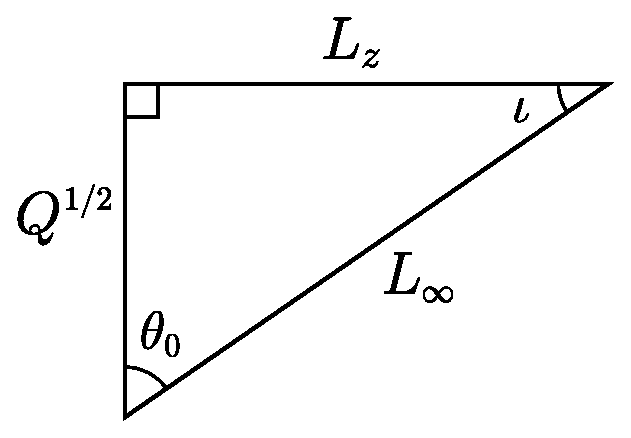
\includegraphics[width=0.25\textwidth]{./images/Triangle}
    \caption{The angular momenta $L_\infty$, $L_z$ and $\sqrt{Q}$ define a right-angled triangle. The acute angles are $\theta_0$, the extremal value of the polar angle, and $\iota$, the orbital inclination \citep{Ryan1996,Glampedakis2002}.}
    \label{fig:L_triangle}
\end{figure}
Introducing a second angular variable \citep{Hughes2000,Drasco2004}
\begin{equation}
\xi = \xi_0\cos^2\chi.
\end{equation}
Over one $2\pi$ period of $\chi$, $\theta$ oscillates from its minimum value to its maximum and back. The geodesic equation for $\chi$ is
\begin{equation}
\varrho^2\diff{\chi}{\tau} = \sqrt{Q + L_z^2}.
\end{equation}

\section{Waveform construction}\label{sec:Kludge}

We can now calculate the geodesic trajectory. The orbiting body is assumed to follow this track exactly; we ignore evolution due to the radiation of energy and angular momentum, which should be negligible for EMRBs as calculated in \apref{evolve}. From this trajectory we calculate the waveform using a semirelativistic approximation \citep{Ruffini1981}: we assume the particle moves along the Kerr geodesic, but radiates as if it were in flat spacetime. This quick-and-dirty technique is known as a numerical kludge (NK), and has been shown to approximate well results computed by more accurate methods \citep{Babak2007}. It is often compared to a bead travelling along a wire. The shape of the wire is set by the Kerr geodesic, but the bead moves along in flat space.

\subsection{The kludge approximation}

Numerical kludge approximations aim to encapsulate the main characteristics of a waveform by using the exact particle trajectory (ignoring inaccuracies from radiative effects and from the particle's self-force), whilst saving on computational time by using approximate waveform generation techniques.

We build an equivalent flat-space trajectory by identifying the Boyer--Lindquist coordinates with a set of flat-space coordinates. We consider two choices:
\begin{enumerate}
\item Identify the Boyer--Lindquist coordinates with flat-space spherical polars $\{r\sub{BL},$ $\theta\sub{BL},$ $\phi\sub{BL}\} \rightarrow \{r\sub{sph}, \theta\sub{sph}, \phi\sub{sph}\}$, then define flat-space Cartesian coordinates \citep{Gair2005, Babak2007}
\begin{equation}
\boldsymbol{x} = \begin{pmatrix}
r\sub{sph} \sin\theta\sub{sph}\cos\phi\sub{sph} \\
r\sub{sph} \sin\theta\sub{sph}\sin\phi\sub{sph} \\
r\sub{sph} \cos\theta\sub{sph}
\end{pmatrix}.
\end{equation}
\item Identify the Boyer--Lindquist coordinates with flat-space oblate-spheroidal coordinates \linebreak $\{r\sub{BL}, \theta\sub{BL}, \phi\sub{BL}\} \rightarrow \{r\sub{ob}, \theta\sub{ob}, \phi\sub{ob}\}$ so that the flat-space Cartesian coordinates are
\begin{equation}
\boldsymbol{x} = \begin{pmatrix}
\sqrt{{r\sub{ob}}^2 + a^2} \sin\theta\sub{ob}\cos\phi\sub{ob} \\
\sqrt{{r\sub{ob}}^2 + a^2} \sin\theta\sub{ob}\sin\phi\sub{ob} \\
r\sub{ob} \cos\theta\sub{ob}
\end{pmatrix}.
\end{equation}
These are appealing because in the limit that $G \rightarrow 0$, where the gravitating mass goes to zero, the Kerr metric in Boyer--Lindquist coordinates reduces to the Minkowski metric in oblate-spheroidal coordinates.
\end{enumerate}
The two coincide for $a \rightarrow 0$ or $r \rightarrow \infty$.

There is no well motivated argument that either coordinate system must yield an accurate GW; their use is justified {\it post facto} by comparison with results obtained from more accurate, and computationally intensive, methods \citep{Gair2005, Babak2007}. The ambiguity in assigning flat-space coordinates reflects the inconsistency of the semirelativistic approximation: the geodesic trajectory was calculated for the Kerr geometry; by moving to flat spacetime we lose the reason for its existence. This should not be regarded as a major problem; it is an artifact of the basic assumption that the shape of the trajectory is important for determining the character of the radiation, but the curvature of the spacetime in the vicinity of the source is not. By binding the particle to the exact geodesic, we ensure that the waveform has spectral components at the correct frequencies, but by assuming flat spacetime for generation of GWs they shall not have the correct amplitudes.

\subsection{The quadrupole--octupole formula}

Now we have a flat-space particle trajectory $x\sub{P}^\mu(\tau)$, we may apply a flat-space wave generation formula. We use the quadrupole--octupole formula to calculate the gravitational strain \citep{Bekenstein1973, Press1977, Yunes2008}
\begin{equation}
h^{jk}(t, \boldsymbol{x}) = -\dfrac{2G}{c^6r}\left(\ddot{I}^{jk} - 2n_i\ddot{S}^{ijk} + n_i\dddot{M}^{ijk}\right)_{t'\, =\, t - r/c},
\label{eq:octupole}
\end{equation}
where an over-dot represents differentiation with respect to time $t$, $t'$ is the retarded time, $r = \left|\boldsymbol{x} - \boldsymbol{x}\sub{P}\right|$ is the radial distance, $\boldsymbol{n}$ is the radial unit vector, and the mass quadrupole ${I}^{jk}$, current quadrupole ${S}^{ijk}$ and mass octupole ${M}^{ijk}$ are defined by
\begin{subequations}
\begin{align}
{I}^{jk}\left(t'\right) = {} & \intd{}{}{{x'}^j{x'}^kT^{00}\left(t', \boldsymbol{x'}\right) }{^3x'};\\
{S}^{ijk}\left(t'\right) = {} & \intd{}{}{{x'}^j{x'}^kT^{0i}\left(t', \boldsymbol{x'}\right)}{^3x'};\\
{M}^{ijk}\left(t'\right)  = {} & \recip{c}\intd{}{}{{x'}^i{x'}^j{x'}^kT^{00}\left(t', \boldsymbol{x'}\right)}{^3x'},
\end{align}
\end{subequations}
for energy-momentum tensor $T^{\mu\nu}$. This is correct for a slowly moving source. It is the familiar quadrupole formula \linebreak[0] (\citealt[section 36.10]{Misner1973}; \citealt[section 17.9]{Hobson2006}), derived from linearized theory, plus the next order terms. For a point mass, $T^{\mu\nu}$ contains a $\delta$-function which allows easy evaluation of the integrals.

Since we are only interested in GWs, we use the transverse-traceless (TT) gauge \citep[box 35.1]{Misner1973}.

\section{Signal detection and analysis}\label{sec:Signal}

\subsection{The LISA detector}\label{sec:Detector}

The classic LISA design is a three arm, space-borne laser interferometer \citep{Bender1998, Danzmann2003}. The arms form an equilateral triangle that rotates as the system's centre of mass follows a circular, heliocentric orbit, trailing $20^{\circ}$ behind the Earth. eLISA has a similar design, but  has only two arms, which are shorter in length, and trails $9^{\circ}$ behind the Earth \citep{Jennrich2011}.

To describe the detector configuration, and to transform from the MBH coordinate system to those of the detector, we use three coordinate systems: those of the BH at the GC $x_\bullet^i$; ecliptic coordinates centred at the solar system (SS) barycentre $x_\odot^i$, and coordinates that co-rotate with the detector $x\sub{d}^i$. The MBH's coordinate system and the SS coordinate system are depicted in \figref{BH_SS}.
\begin{figure}
\centering
 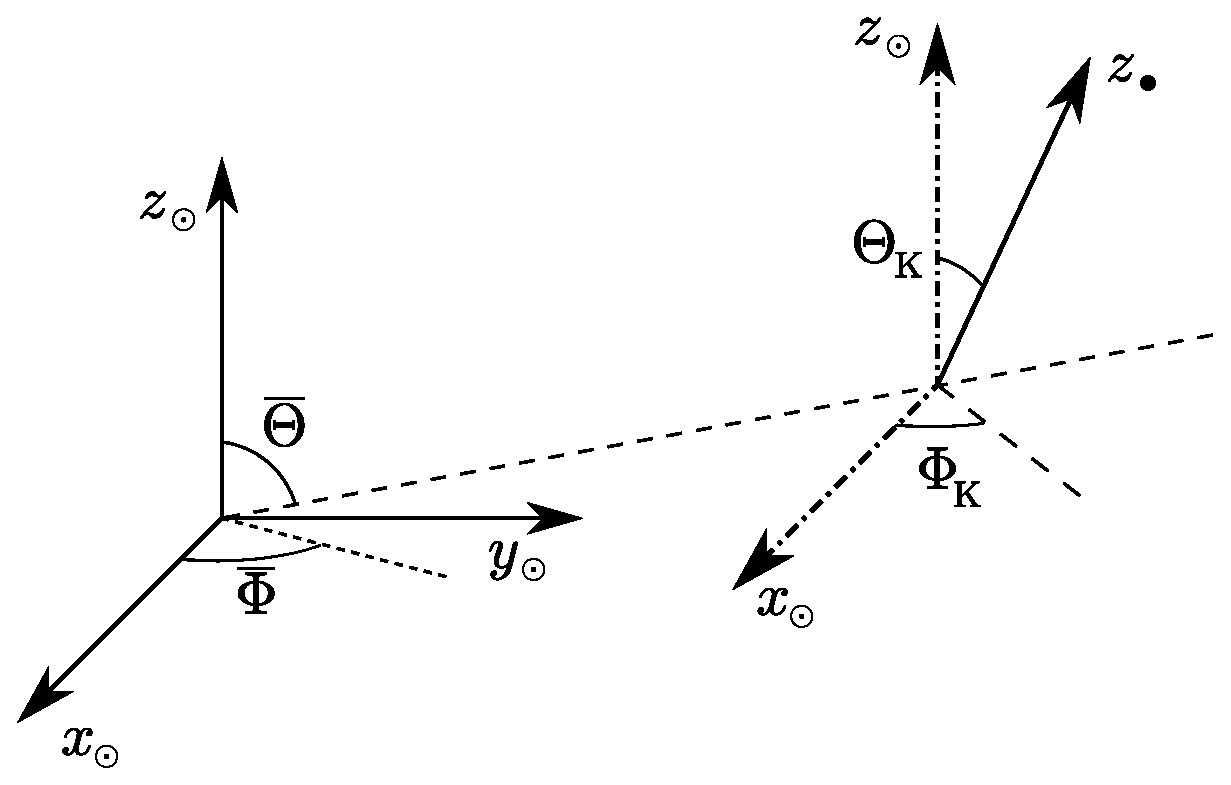
\includegraphics[width=0.42\textwidth]{./images/BH_SS_angles}
    \caption{The relationship between the MBH's coordinate system $x_\bullet^i$ and the SS coordinate system $x_\odot^i$. The MBH's spin axis is aligned with the $z_\bullet$-axis. The orientation of the MBH's $x$- and $y$-axes is arbitrary. We choose $x_\bullet$ to be orthogonal to the direction to the SS.}
   \label{fig:BH_SS}
\end{figure}
The mission geometry for LISA and eLISA is shown in \figref{SS_LISA}.
\begin{figure}
\centering
 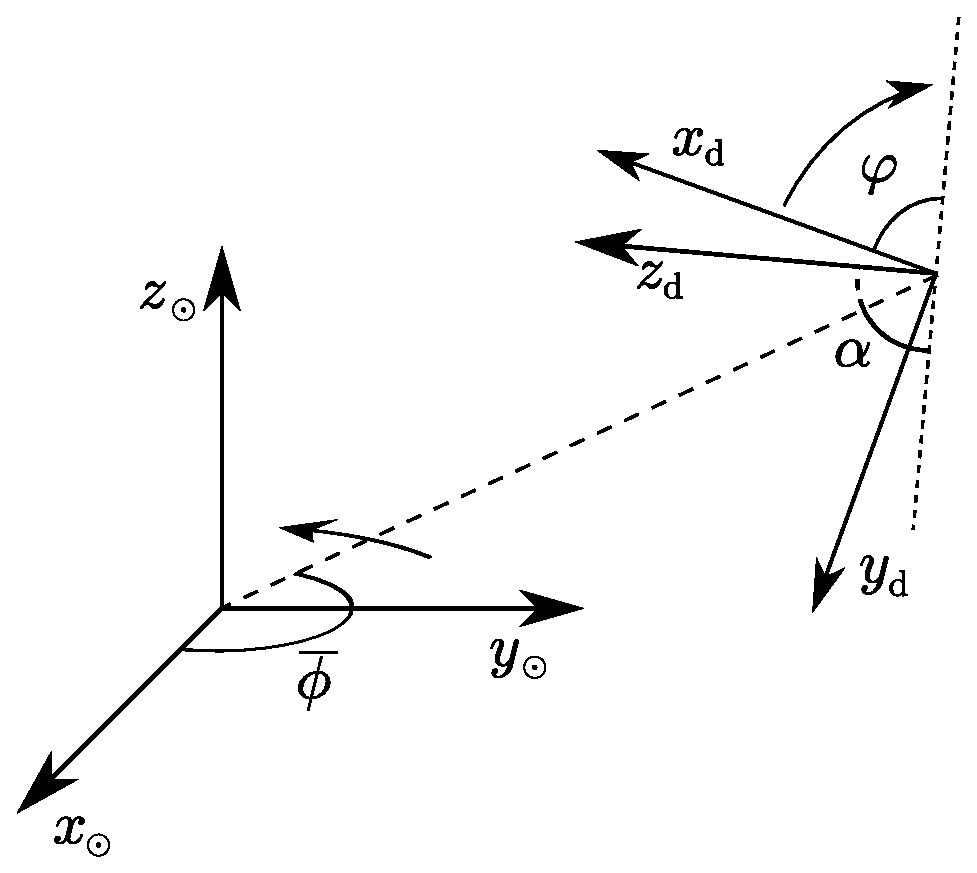
\includegraphics[width=0.32\textwidth]{./images/SS_LISA}
    \caption{The relationship between the detector coordinates $x\sub{d}^i$ and the ecliptic coordinates of the SS $x_\odot^i$ \citep{Bender1998, Jennrich2011}. The detector inclination is $\alpha = 60^{\circ}$.}
   \label{fig:SS_LISA}
\end{figure}
We define the detector coordinates such that the detector-arms lie in the $x\sub{d}$-$y\sub{d}$ plane as in \citet{Cutler1998}. We have computed the waveforms in the MBH's coordinates, but it is simplest to describe the measured signal using the detector's coordinates.

The strains measured in the three arms can be combined such that LISA behaves as a pair of $90^{\circ}$ interferometers at $45^{\circ}$ to each other, with signals scaled by ${\sqrt{3}}/{2}$ \citep{Cutler1998}. We denote the two detectors as I and II and use vector notation $\boldsymbol{h}(t) = \left(h\sub{I}(t), h\sub{II}(t)\right) = \left\{h_A(t)\right\}$ to represent signals from both detectors. As eLISA only has two arms it functions as a single detector, in this case $\left\{h_A(t)\right\} = h\sub{I}(t)$.

\subsection{Frequency domain formalism}

Having constructed the GW $\boldsymbol{h}(t)$ that shall be incident upon the detector, we may consider how to analyse the waveform and extract the information it contains. We briefly recap GW signal analysis, with application to LISA. A more complete discussion can be found in \citet{Finn1992} and \citet{Cutler1994}. Adaption for eLISA requires a substitution of the noise distribution, and the removal of the sum over data channels, since it would only have one.

The measured strain $\boldsymbol{s}(t)$ is the combination of the signal and the detector noise
\begin{equation}
\boldsymbol{s}(t) = \boldsymbol{h}(t) + \boldsymbol{n}(t);
\end{equation}
we assume the noise $n_A(t)$ is stationary and Gaussian, and that noise in the two detectors is uncorrelated, but shares the same characterisation \citep{Cutler1998}.

The properties of the noise allow us to define a natural inner product and associated distance on the space of signals \citep{Cutler1994}
\begin{equation}
\innerprod{\boldsymbol{g}}{\boldsymbol{k}} = 2\intd{0}{\infty}{\dfrac{\tilde{g}_A^\ast(f)\tilde{k}_A(f) + \tilde{g}_A(f)\tilde{k}_A^\ast(f)}{S_{n}(f)}}{f},
\label{eq:inner}
\end{equation}
introducing Fourier transforms
\begin{equation}
\tilde{g}(f) = \mathscr{F}\{g(t)\} = \intd{-\infty}{\infty}{g(t)\exp(2\pi i ft)}{t},
\end{equation}
and $S_{n}(f)$ is the noise spectral density. The inner product is derived in \apref{inner-prod}. The signal-to-noise ratio is approximately
\begin{equation}
\rho[\boldsymbol{h}] = \innerprod{\boldsymbol{h}}{\boldsymbol{h}}^{1/2}.
\label{eq:SNR}
\end{equation}
The probability of a particular realization of noise $\boldsymbol{n}(t) = \boldsymbol{n}_0(t)$ is
\begin{equation}
p(\boldsymbol{n}(t) = \boldsymbol{n}_0(t)) \propto \exp\left[-\recip{2}\innerprod{\boldsymbol{n}_0}{\boldsymbol{n}_0}\right].
\end{equation}
Thus, if the incident waveform is $\boldsymbol{h}(t)$, the probability of measuring signal $\boldsymbol{s}(t)$ is
\begin{equation}
p(\boldsymbol{s}(t)|\boldsymbol{h}(t)) \propto \exp\left[-\recip{2}\innerprod{\boldsymbol{s}-\boldsymbol{h}}{\boldsymbol{s}-\boldsymbol{h}}\right].
\label{eq:sig_prob}
\end{equation}

\subsection{The noise curve}\label{sec:Noise}

LISA's noise has two sources: instrumental noise and confusion noise, primarily from WD binaries. The latter may be divided into contributions from galactic and extragalactic binaries. In this work we use the noise model of \citet{Barack2004}. The shape of the noise curve can be seen in \figref{Noise}. The instrumental noise dominates at both high and low frequencies. The confusion noise is important at intermediate frequencies, and is responsible for the cusp around $10^{-3}\units{Hz}$. eLISA shares the same sources of noise, but is less affected by confusion \citep{Jennrich2011}. Its sensitivity regime is shifted to higher frequencies because of the shorter arm length.
\begin{figure}[!htp]
\centering
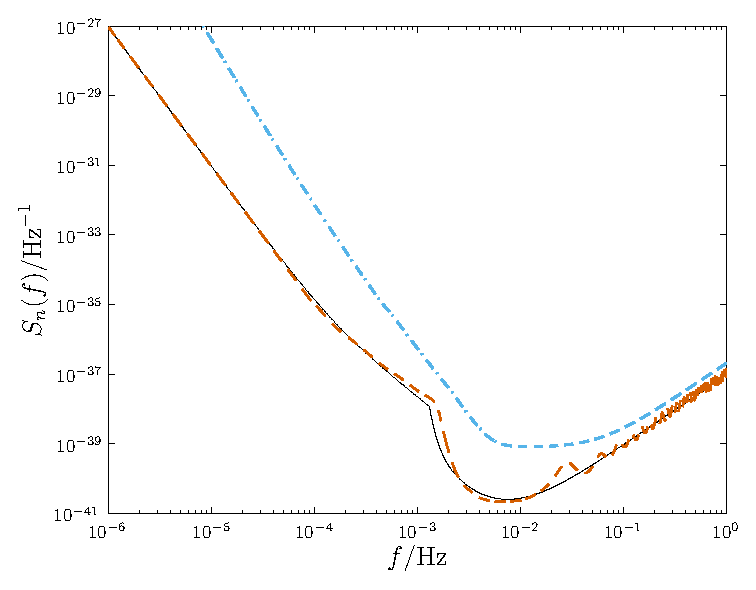
\includegraphics[width=0.6\textwidth]{./images/Fig_Noise}
\caption{The detector noise curves. The solid line indicates the analytic approximation of \citet{Barack2004} used in this work. For comparison, the dashed line is from the online LISA sensitivity curve generator (\url{http://www.srl.caltech.edu/~shane/sensitivity/}; \citealt*{Larson2000, Larson2002}). For bursts from the Galactic Centre we are most interested in the low-frequency region where the two curves are the same. The dot--dashed line shows the eLISA noise curve.}
\label{fig:Noise}
\end{figure}

\subsection{Window functions}

There is one remaining complication regarding signal analysis: as we are Fourier transforming a finite signal we encounter spectral leakage; a contribution from large amplitude spectral components leaks into surrounding components (sidelobes), obscuring and distorting the spectrum at these frequencies \citep{Harris1978}. This is an inherent problem with finite signals; it shall be as much of a problem when analysing signals from an actual mission as it is here. To mitigate, but unfortunately not eliminate, these effects, the time-domain signal can be multiplied by a window function. These are discussed in detail in \apref{window}. We adopt the Nuttall four-term window with continuous first derivative \citep{Nuttall1981} for our results. This should not affect the accuracy of our conclusions.

\section{Energy spectra}\label{sec:Energy}

To check the NK waveforms, we compare the energy spectra calculated from these with those obtained from the classic treatment of \citet{Peters1963} and \citet{Peters1964}. This calculates GW emission for Keplerian orbits in flat spacetime, assuming only quadrupole radiation. The spectrum produced should be similar to that obtained from the NK in weak fields, that is for large periapses; we do not expect an exact match because of the differing input physics and varying approximations.

In addition to using the energy spectrum, we also use the total energy flux. This contains less information than the spectrum; however, \citet{Martel2004} has calculated results for parabolic orbits in Schwarzschild spacetime using time-domain BH perturbation theory. These should be more accurate than results calculated using the Peters and Mathews formalism.

As we are considering Schwarzschild spacetime, the two NK coordinate choices coincide and there is no need to differentiate between them. In general, we do not intend to use the kludge waveforms to calculate an accurate energy flux: this would be inconsistent as we assume the orbits do not evolve with time. We only calculate the energy flux as a sanity check, to confirm that the kludge approximation is consistent with other approaches.

\subsection{Kludge spectrum}

A GW in the TT gauge has an effective energy-momentum tensor \citep[section 35.15]{Misner1973}
\begin{equation}
T_{\mu\nu} = \dfrac{c^4}{32\pi G}\left\langle\partial_\mu h_{ij} \partial_\nu h^{ij}\right\rangle,
\end{equation}
where $\langle\ldots\rangle$ indicates averaging over several wavelengths or periods. The energy flux through a sphere of radius $R$ is
\begin{equation}
\diff{E}{t} = \dfrac{c^3}{32\pi G} R^2 \int{\dd\Omega}\left\langle\diff{h_{ij}}{t}\diff{h^{ij}}{t}\right\rangle,
\end{equation}
with $\int{\dd\Omega}$ representing integration over all solid angles. From \eqnref{octupole} the waves have a $1/{r}$ dependence; if we define
\begin{equation}
h_{ij} = \dfrac{H_{ij}}{r},
\end{equation}
we see the flux is independent of $R$, as required for energy conservation, and
\begin{equation}
\diff{E}{t} = \dfrac{c^3}{32\pi G} \int{\dd\Omega}\left\langle\diff{H_{ij}}{t}\diff{H^{ij}}{t}\right\rangle.
\end{equation}
Integrating to find the total energy emitted
\begin{equation}
E = \dfrac{c^3}{32\pi G} \int{\dd\Omega}\int_{-\infty}^{\infty}{\dd t} \, \diff{H_{ij}}{t}\diff{H^{ij}}{t}.
\label{eq:integrate_E}
\end{equation}
Since we are considering all time, the localization of the energy is no longer of importance and it is unnecessary to average over several periods. Switching to Fourier representation $\widetilde{H}_{ij}(f) = \mathscr{F}\left\{H_{ij}(t)\right\}$,
\begin{equation}
E = \dfrac{\pi c^3}{4 G} \int{\dd\Omega}\int_{0}^{\infty}{\dd f} \, f^2 \widetilde{H}^{ij}(f)\widetilde{H}_{ij}^*(f),
\label{eq:total_E}
\end{equation}
using $\widetilde{H}_{ij}^*(f) = \widetilde{H}_{ij}(-f)$ as the signal is real. From this we identify the energy spectrum as
\begin{align}
\diff{E}{f} = \dfrac{\pi c^3}{4 G} \intd{}{}{}{\Omega} \, f^2 \widetilde{H}^{ij}(f)\widetilde{H}_{ij}^*(f).
\label{eq:NK_dEdf}
\end{align}

\subsection{Peters and Mathews spectrum}\label{sec:P-M}

For an orbit of eccentricity $e$ with periapse radius $r\sub{p}$, \citet{Peters1963} give the power radiated into the $n$-th harmonic of the orbital angular frequency as
\begin{equation}
P(n) = \dfrac{32}{5}\dfrac{G^4}{c^5}\dfrac{M_\bullet^2\mu^2(M_\bullet + \mu)(1-e)^5}{r\sub{p}^5}g(n,e),
\label{eq:PM_P}
\end{equation}
where the function $g(n,e)$ is defined in terms of Bessel functions of the first kind
\begin{align}
g(n,e) = {} & \dfrac{n^4}{32}\left\{\left[J_{n-2}(ne) - 2eJ_{n-1}(ne) + \dfrac{2}{n}J_n(ne) + 2eJ_{n+1}(ne) - J_{n+2}(ne)\right]^2 \right. \nonumber \\*
 & + \left. \left(1 - e^2\right)\left[J_{n-2}(ne) - 2J_n(ne) + J_{n+2}(ne)\right]^2 + \dfrac{4}{3n^2}\left[J_n(ne)\right]^2\right\}.
% Line breaks follow Peters and Mathews paper
\end{align}
The Keplerian orbital frequency is
\begin{equation}
\omega_1^2 = \dfrac{G(M_\bullet + \mu)(1 - e)^3}{r\sub{p}^3} = (1 - e)^3\omega\sub{c}^2,
\label{eq:Kepler_freq}
\end{equation}
where $\omega\sub{c}$ is defined as the angular frequency of a circular orbit of radius $r\sub{p}$. The energy radiated per orbit into the $n$-th harmonic, that is at frequency $\omega_n = n\omega_1$, is
\begin{equation}
E(n) = \dfrac{2\pi}{\omega_1}P(n);
\label{eq:E(n)}
\end{equation}
as $e \rightarrow 1$ for a parabolic orbit, $\omega_1 \rightarrow 0$ as the orbital period becomes infinite. The energy radiated per orbit is then the total energy radiated. The spacing of harmonics is $\Delta\omega = \omega_1$, giving energy spectrum
\begin{equation}
\left.\diff{E}{\omega}\right|_{\omega_n}\omega_1 = E(n).
\end{equation}
Changing to linear frequency $2\pi f = \omega$,
\begin{align}
\left.\diff{E}{f}\right|_{f_n}  = {} & \dfrac{128\pi^2}{5}\dfrac{G^3}{c^5}\dfrac{M_\bullet^2\mu^2}{r\sub{p}^2}(1-e)^2g(n,e) \\*
  = {} & \dfrac{4\pi^2}{5}\dfrac{G^3}{c^5}\dfrac{M_\bullet^2\mu^2}{r\sub{p}^2}\ell(n,e),
\label{eq:PM_spectrum}
\end{align}
where the function $\ell(n,e)$ is defined in the last line. For a parabolic orbit, we must take the limit of $\ell(n,e)$ as $e \rightarrow 1$.

We simplify $\ell(n,e)$ using the recurrence formulae \citep[section 2.12]{Watson1995}
\begin{align}
J_{\nu-1}(z) + J_{\nu+1}(z)  = {} & \dfrac{2\nu}{z}J_\nu(z)\\*
J_{\nu-1}(z) - J_{\nu+1}(z)  = {} & 2J'_\nu(z),\label{eq:J_derivative}
\end{align}
and eliminate $n$ using
\begin{equation}
n = \dfrac{\omega_n}{\omega_1} = (1-e)^{-3/2}\tilde{f},
\end{equation}
where $\tilde{f} = \omega_n/\omega\sub{c} = f_n/f\sub{c}$ is a dimensionless frequency. To find the limit we define two new functions \citep{Berry2010}
\begin{equation}
A(\tilde{f}) = \lim_{e\rightarrow 1}\left\{\dfrac{J_n(ne)}{(1-e)^{1/2}}\right\}; \quad B(\tilde{f}) = \lim_{e\rightarrow 1}\left\{\dfrac{J'_n(ne)}{1-e}\right\}.
\end{equation}
To give a well-defined energy spectrum, both of these must be finite.

The Bessel function has an integral representation
\begin{equation}
J_\nu(z) = \recip{\pi}\intd{0}{\pi}{\cos(\nu\vartheta - z\sin\vartheta)}{\vartheta};
\end{equation}
we want the limit of this for $\nu \rightarrow \infty$, $z \rightarrow \infty$, with $z \leq \nu$. Using the stationary phase approximation, the dominant contribution to the integral comes from the regime in which the argument of the cosine is approximately zero \citep[sections 8.2, 8.43]{Watson1995}:
\begin{align}
J_\nu(z)  \sim {} & \recip{\pi}\intd{0}{\pi}{\cos\left(\nu\vartheta - z\vartheta + \dfrac{z}{6}\vartheta^3\right)}{\vartheta}\\*
  \sim {} & \recip{\pi}\intd{0}{\infty}{\cos\left(\nu\vartheta - z\vartheta + \dfrac{z}{6}\vartheta^3\right)}{\vartheta};
\end{align}
this last expression is an Airy integral and has a standard form \citep[section 6.4]{Watson1995}
\begin{equation}
\intd{0}{\infty}{\cos(t^3 + xt)}{t} = \dfrac{\sqrt{x}}{3}K_{1/3}\left(\dfrac{2x^{3/2}}{3^{3/2}}\right),
\end{equation}
where $K_\nu(z)$ is a modified Bessel function of the second kind. Using this to evaluate the limit gives
\begin{equation}
J_\nu(z) \sim \recip{\pi}\sqrt{\dfrac{2(\nu - z)}{3z}}K_{1/3}\left(\dfrac{2^{3/2}}{3}\sqrt{\dfrac{(\nu -z)^3}{z}}\right).
\label{eq:J_nu}
\end{equation}
For our case,
\begin{equation}
J_n(ne) \sim \recip{\pi}\sqrt{\dfrac{2}{3}}(1-e)^{1/2}K_{1/3}\left(\dfrac{2^{3/2}\tilde{f}}{3}\right),
\end{equation}
and the first limiting function is well defined,
\begin{equation}
A(\tilde{f}) = \recip{\pi}\sqrt{\dfrac{2}{3}}K_{1/3}\left(\dfrac{2^{3/2}\tilde{f}}{3}\right).
\end{equation}

To find the derivative we combine equations \eqref{eq:J_derivative} and \eqref{eq:J_nu}, and expand to lowest order yielding
\begin{align}
J'_n(ne) \sim {} & -\dfrac{1}{2\pi}\sqrt{\dfrac{2}{3}}(1-e)\left[2^{3/2}K'_{1/3}\left(\dfrac{2^{3/2}\tilde{f}}{3}\right) + \recip{\tilde{f}}K_{1/3}\left(\dfrac{2^{3/2}\tilde{f}}{3}\right)\right].
\end{align}
We may re-express the derivative using the recurrence formula \citep[section 3.71]{Watson1995}
\begin{equation}
K_{\nu-1}(z) + K_{\nu+1}(z) = -2K'_\nu(z)
\end{equation}
to give
\begin{align}
J'_n(ne)  \sim {} & \dfrac{1-e}{\sqrt{3}\pi}\left[K_{-2/3}\left(\dfrac{2^{3/2}\tilde{f}}{3}\right) + K_{4/3}\left(\dfrac{2^{3/2}\tilde{f}}{3}\right) - \recip{\sqrt{2}\tilde{f}}K_{1/3}\left(\dfrac{2^{3/2}\tilde{f}}{3}\right)\right].
\end{align}
And so finally we obtain the well-defined
\begin{align}
B(\tilde{f})  = {} & \recip{\sqrt{3}\pi}\left[K_{-2/3}\left(\dfrac{2^{3/2}\tilde{f}}{3}\right) + K_{4/3}\left(\dfrac{2^{3/2}\tilde{f}}{3}\right) - \recip{\sqrt{2}\tilde{f}}K_{1/3}\left(\dfrac{2^{3/2}\tilde{f}}{3}\right)\right].
\end{align}

Having obtained expressions for $A(\tilde{f})$ and $B(\tilde{f})$ in terms of standard functions, we can calculate the energy spectrum for a parabolic orbit. From \eqnref{PM_spectrum}
\begin{equation}
\diff{E}{f} = \dfrac{4\pi^2}{5}\dfrac{G^3}{c^5}\dfrac{M_\bullet^2\mu^2}{r\sub{p}^2}\ell\left(\dfrac{f}{f\sub{c}}\right),
\label{eq:PM_dEdf}
\end{equation}
where we have used the limit
\begin{align}
\ell(\tilde{f})  = {} & \left[8\tilde{f}^2B(\tilde{f}) - 2\tilde{f}A(\tilde{f})\right]^2 + \left(128\tilde{f}^4 + \dfrac{4\tilde{f}^2}{3}\right)\left[A(\tilde{f})\right]^2.
\label{eq:ell}
\end{align}
This agrees with the $e = 1$ result of \citet{Turner1977}, which was computed by direct integration along unbound orbits. \Figref{ell} shows how $\ell(n,e)$ changes with eccentricity including our result for a parabolic encounter. Although more power is radiated into higher harmonics, the peak of the spectrum does not move much: it is always between $f = f\sub{c}$ and $f = 2 f\sub{c}$, with $f = 2 f\sub{c}$ for $e = 0$ and $f \simeq 1.637 f\sub{c}$ for $e = 1$.
\begin{figure}%[!htp]
\centering
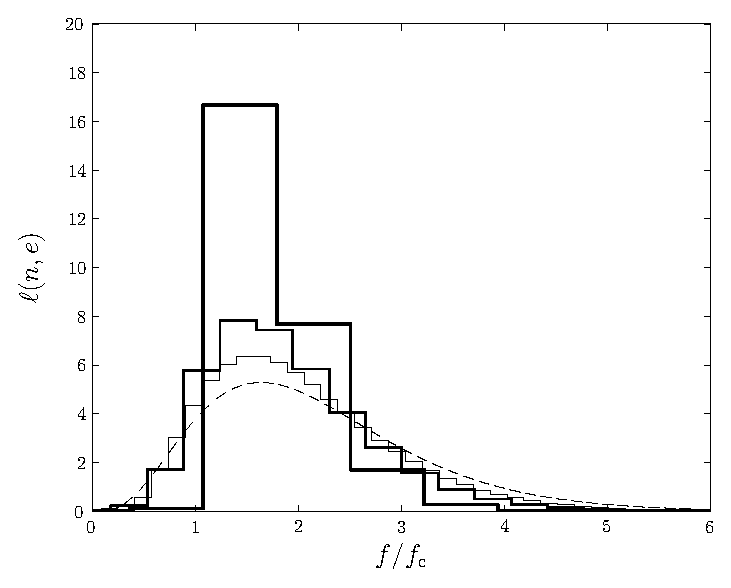
\includegraphics[width=0.6\textwidth]{./images/Fig_ell}
\caption{The relative energy (per orbit) spectrum $\ell(n,e)$ for $e = 0.2$ (heavy line), $e = 0.5$ (medium line), $e = 0.7$ (light line), and the limiting result for $e = 1$ (dashed line) versus frequency. Compare with figure 3 of \citet{Peters1963}.}
\label{fig:ell}
\end{figure}

\subsubsection{Total Energy}

To check the validity of this limit we can calculate the total energy radiated by integrating \eqnref{PM_dEdf} over all frequencies, or by summing the energy radiated into each harmonic. These must yield the same result. Summing:
\begin{equation}
E\sub{sum} = \dfrac{64\pi}{5}\dfrac{G^3}{c^5}\dfrac{M_\bullet^2\mu^2}{r\sub{p}^2}\omega\sub{c}(1-e)^{7/2}\sum_n g(n,e),
\end{equation}
where we have used equations \eqref{eq:PM_P}, \eqref{eq:Kepler_freq} and \eqref{eq:E(n)}. \citet{Peters1963} provide the result
\begin{equation}
\sum_n g(n,e) = \dfrac{1 + (73/24)e^2 + (37/96)e^4}{(1-e^2)^{7/2}}.
\end{equation}
Using this,
\begin{equation}
E\sub{sum} = \dfrac{64\pi}{5}\dfrac{G^3}{c^5}\dfrac{M_\bullet^2\mu^2}{r\sub{p}^2}\omega\sub{c}\dfrac{1 + (73/24)e^2 + (37/96)e^4}{(1+e)^{7/2}},
\end{equation}
which is perfectly well behaved as $e \rightarrow 1$,
\begin{equation}
E\sub{sum} = \dfrac{85\pi}{2^{5/2}3}\dfrac{G^3}{c^5}\dfrac{M_\bullet^2\mu^2}{r\sub{p}^2}\omega\sub{c}.
\label{eq:PM_total}
\end{equation}
Integrating the energy spectrum \eqnref{PM_dEdf} gives
\begin{equation}
E\sub{int} = \dfrac{2\pi}{5}\dfrac{G^3}{c^5}\dfrac{M_\bullet^2\mu^2}{r\sub{p}^2}\omega\sub{c}\intd{0}{\infty}{\ell(\tilde{f})}{\tilde{f}}.
\end{equation}
The integral can be evaluated numerically as
\begin{equation}
\intd{0}{\infty}{\ell(\tilde{f})}{\tilde{f}} = 12.5216858\ldots = \dfrac{425}{2^{7/2}3}.
\end{equation}
The two total energies are consistent, $E\sub{int} = E\sub{sum}$.

\subsection{Comparison}

Two energy spectra are plotted in \figref{Energy} for orbits with periapses of $r\sub{p} = 15.0 r\sub{g}$, $30.0 r\sub{g}$ and $60.0 r\sub{g}$.
\begin{figure}%[!htp]
  \centering
   \subfigure[$r\sub{p} = 15.0 r\sub{g}$, log-log plot.]{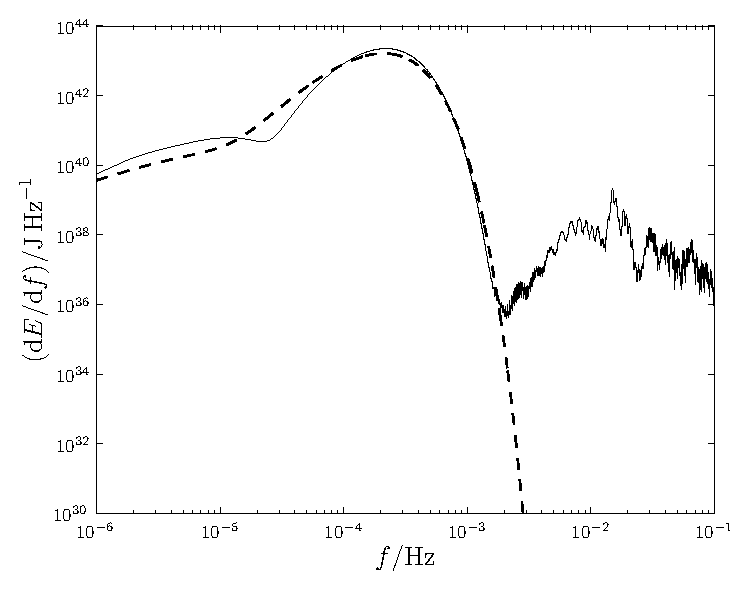
\includegraphics[width=0.48\textwidth]{./images/Fig_Loglog_E_15}} \quad
   \subfigure[$r\sub{p} = 15.0 r\sub{g}$, log-linear plot.]{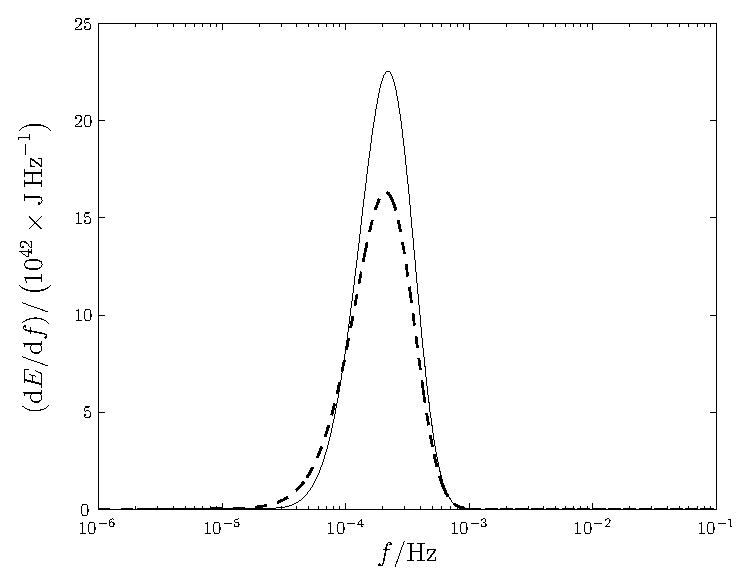
\includegraphics[width=0.48\textwidth]{./images/Fig_Loglin_E_15}} \\
   \subfigure[$r\sub{p} = 30.0 r\sub{g}$, log-log plot.]{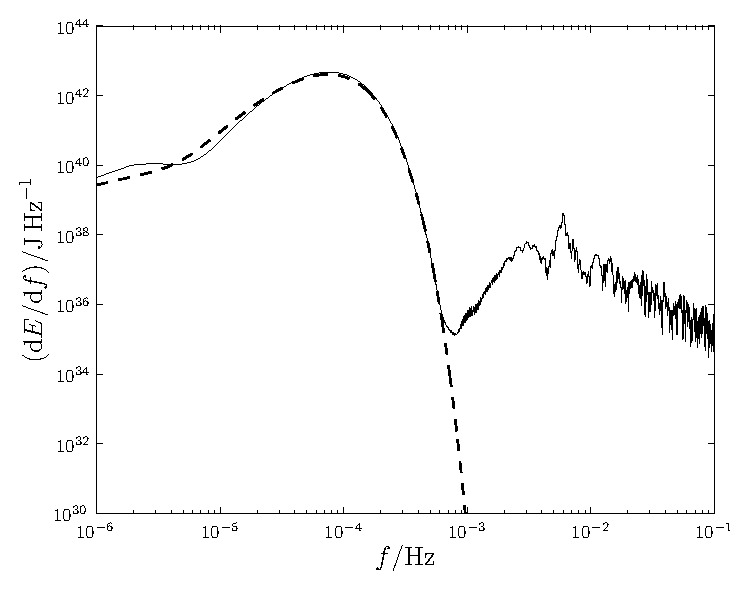
\includegraphics[width=0.48\textwidth]{./images/Fig_Loglog_E_30}} \quad
   \subfigure[$r\sub{p} = 30.0 r\sub{g}$, log-linear plot.]{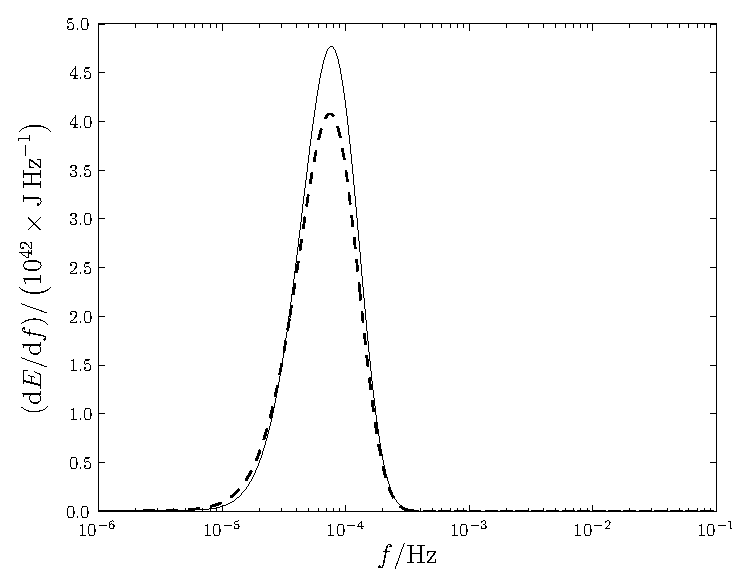
\includegraphics[width=0.48\textwidth]{./images/Fig_Loglin_E_30}} \\
   \subfigure[$r\sub{p} = 60.0 r\sub{g}$, log-log plot.]{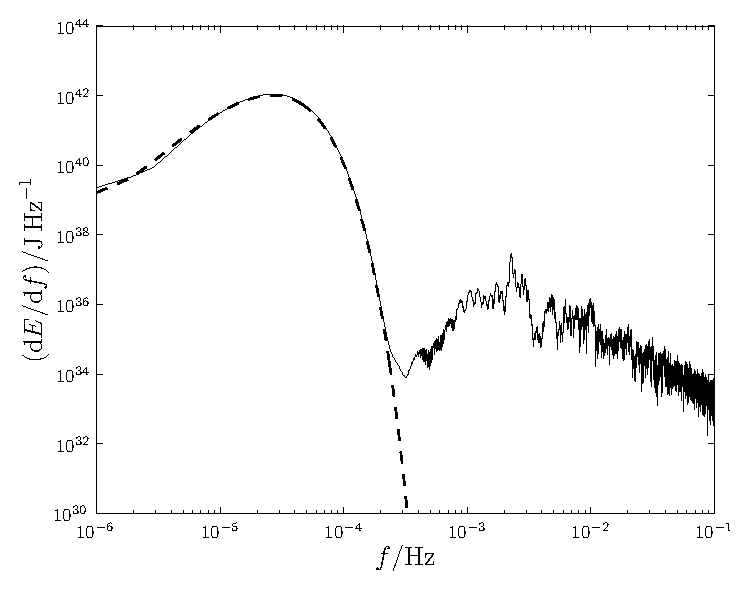
\includegraphics[width=0.48\textwidth]{./images/Fig_Loglog_E_60}} \quad
   \subfigure[$r\sub{p} = 60.0 r\sub{g}$, log-linear plot.]{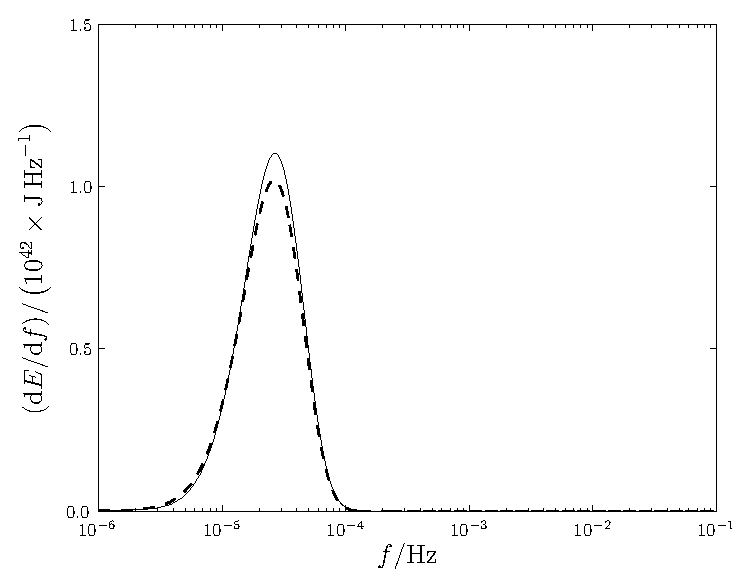
\includegraphics[width=0.48\textwidth]{./images/Fig_Loglin_E_60}}
    \caption{Energy spectra for a parabolic orbit of a $\mu = 10 M_\odot$ object about a Schwarzschild BH with $M_\bullet = 4.31 \times 10^6 M_\odot$. The spectra calculated from the NK waveform is shown by the solid line and the Peters and Mathews flux is indicated by the dashed line. The NK waveform includes octupole contributions. The high frequency tail is the result of spectral leakage.}
    \label{fig:Energy}
\end{figure}
The two spectra appear to be in good agreement, showing the same general shape in the weak-field limit. The NK spectrum is more tightly peaked, but is always within a factor of $2$ at the apex. The peak of the spectrum is shifted to a marginally higher frequency in the NK spectrum primarily because of the addition of the current quadrupole and mass octupole terms.

Comparing the total energy fluxes, ratios of the various energies are plotted in \figref{Energy_ratio}.
\begin{figure}%[!htp]
  \centering
   \subfigure[Versus periapsis]{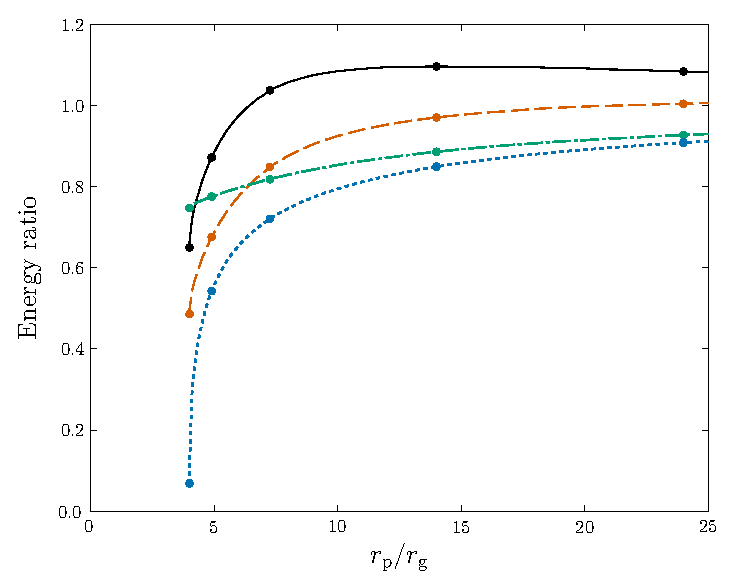
\includegraphics[width=0.475\textwidth]{./images/Fig_Energy_ratio_peri}} \quad
   \subfigure[Versus amount of rotation]{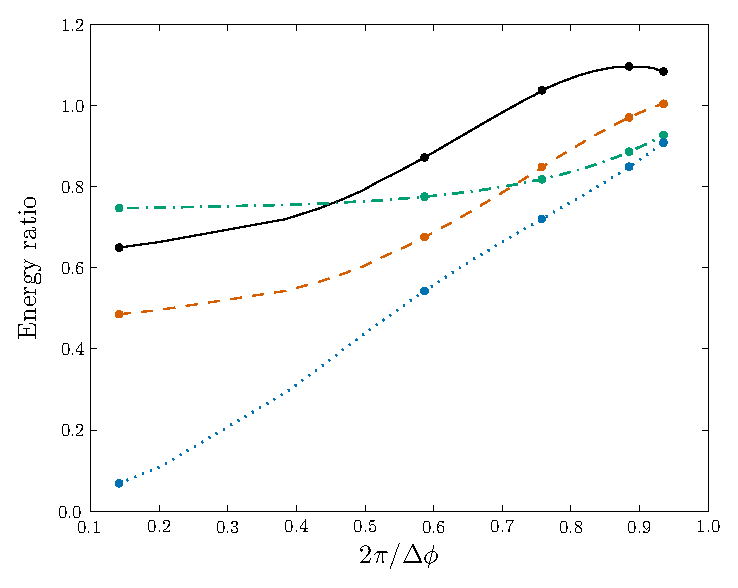
\includegraphics[width=0.475\textwidth]{./images/Fig_Energy_ratio_orbit}}
    \caption{Ratios of energies as a function of periapsis $r\sub{p}$ and $2\pi$ divided by the total angle of rotation in one orbit $\Delta\phi$ ($2\pi/\Delta\phi = 1$ for a Keplerian orbit). The solid line shows the ratio of the numerical kludge and Martel energies $E\sub{NK}/E\sub{M}$; the dashed line shows the ratio of the NK energy calculated using only the mass quadrupole term and the Martel energy $E\sub{NK(Q)}/E\sub{M}$; the dot--dashed line shows the ratio of the quadrupole and quadrupole--octupole NK energies $E\sub{NK(Q)}/E\sub{NK}$, and the dotted line shows the ratio of the Peters and Mathews and quadrupole NK energies $E\sub{PM}/E\sub{NK(Q)}$. The spots show the mapping between the two abscissa scales. Compare with figure 4 of \citet{Gair2005}.}
  \label{fig:Energy_ratio}
\end{figure}
We introduce an additional energy here, the quadrupole NK energy $E\sub{NK(Q)}$. This allows easier comparison with the Peters and Mathews energy which includes only quadrupole radiation. It can be calculated in three ways:
\begin{enumerate}
\item Inserting the waveform $\widetilde{h}(f)$ generated including only the mass quadrupole term in \eqnref{octupole} into \eqnref{total_E} and integrating. This is equivalent to the method used to calculate $E\sub{NK}$.
\item Numerically integrating the quadrupole GW luminosity (\citealt{Misner1973}, section 36.7; \citealt{Hobson2006}, section 18.7)
\begin{equation}
E = \dfrac{G}{5c^9}\intd{}{}{\dddot{\Ibar}_{ij}\dddot{\Ibar}^{ij}}{t},
\label{eq:E_quad}
\end{equation}
where $\Ibar_{ij} = I_{ij} - (1/3)I\delta_{ij}$ is the reduced mass quadrupole tensor. We can obtain this from \eqnref{integrate_E}, by integrating over all angles when the waveform only contains the mass quadrupole component. This has the advantage of avoiding the effects of spectral leakage or the influence of window functions.
\item Using the analytic expressions for the integral \eqnref{E_quad} from appendix A of \citet{Gair2005}. The expressions are included in \apref{energy}.
\end{enumerate}
All three agree to within computational error. No difference is visible on the scale plotted in \figref{Energy_ratio}. This demonstrates the validity of the code.

We have used the amount of rotation $\Delta\phi$ as a convenient measure for the abscissa. For an equatorial orbit in Kerr spacetime,
\begin{align}
\Delta\phi  = {} & 2\intd{r\sub{p}}{\infty}{\diff{\phi}{r}}{r} = \sqrt{\dfrac{2}{M_\bullet}}L_z\intd{r\sub{p}}{\infty}{\dfrac{r^2 - 2M_\bullet(1 - a/L_z)r}{(r^2 - 2M_\bullet r + a^2)w}}{r},
\end{align}
where
\begin{equation}
w^2 = r^3 - \dfrac{L_z^2}{2M_\bullet}r^2 + (L_z - a)^2r;
\end{equation}
$L_z$ is the specific angular momentum about the $z$-axis; $a$ is the spin parameter, and we have adopted units with $G = c = 1$. We shall find it useful to define
\begin{equation}
r_\pm = M_\bullet \pm \sqrt{M_\bullet^2 - a^2},
\end{equation}
and the two nonzero roots of the cubic $w^2$
\begin{equation}
r_{\mathrm{p},\,1} = \dfrac{L_z^2}{4M_\bullet} \pm \sqrt{\dfrac{L_z^4}{16M_\bullet^2} - (L_z -a)^2};
\end{equation}
the periapsis is the larger root $r\sub{p} > r_1$. This equation implicitly gives $L_z$ as a function of $r\sub{p}$. The integral may be rewritten as
\begin{equation}
\Delta\phi = \sqrt{\dfrac{2}{M}}L_z\intd{r\sub{p}}{\infty}{\recip{w}\left(1 + \dfrac{\alpha_+}{r-r_+} + \dfrac{\alpha_-}{r-r_-}\right)}{r},
\end{equation}
where
\begin{equation}
\alpha_\pm = \pm\dfrac{2Mar_\pm - a^2L_z}{2L_z\sqrt{M^2-a^2}}.
\end{equation}
This may be evaluated using elliptic integrals \citep[3.131.8, 3.137.8]{Gradshteyn2000}
\begin{equation}
\Delta\phi = 2 L_z \sqrt{\dfrac{2}{r\sub{p}M}}\left[\dfrac{\alpha_+}{r_+}\Pi\left(\dfrac{r_+}{r\sub{p}}\middle|\dfrac{r_1}{r\sub{p}}\right) + \dfrac{\alpha_-}{r_-}\Pi\left(\dfrac{r_-}{r\sub{p}}\middle|\dfrac{r_1}{r\sub{p}}\right)\right],
\end{equation}
where $\Pi(n|m) = \int_{0}^{\pi/2}{\dd\vartheta/(1-n\sin^2\vartheta)\sqrt{1-m\sin^2\vartheta}}$ is the complete elliptic integral of the third kind. In the limit of $a \rightarrow 0$ we recover the Schwarzschild result \citep{Cutler1994}
\begin{equation}
\Delta\phi =  2 L_z\sqrt{\dfrac{2}{r\sub{p}M}}K\left(\dfrac{r_1}{r\sub{p}}\right),
\end{equation}
where $K(m) = \int_{0}^{\pi/2}{\dd\vartheta/\sqrt{1-m\sin^2\vartheta}}$ is the complete elliptic integral of the first kind.

The ratios all tend towards one in the weak field, as required, but differences become more pronounced in the strong field. The NK energy is larger than the Peters and Mathews result $E\sub{PM}$. This behaviour has been seen before for high eccentricity orbits about a non-spinning BH \citep{Gair2005}. It may be explained by considering the total path length for the different orbits: the Peters and Mathews spectrum assumes a Keplerian orbit, the orbit in Kerr geometry rotates more than this. The greater path length leads to increased emission of GWs and a larger energy flux. Our bead must travel further along its wire. A good proxy for the path length is the angle of rotation $\Delta\phi$; this is $2\pi$ for a Keplerian orbit, in Kerr the angle should be $2\pi$ in the limit of an infinite periapsis, whereas for a periapsis small enough that the orbit shows zoom--whirl behaviour, the total angle may be many times $2\pi$. There is a reasonable correlation between the amount of rotation $2\pi/\Delta\phi$ and the ratio of energies.

Error in the NK energy compared with the time-domain BH perturbation theory results of Martel comes from two sources: the neglecting of higher order multipole contributions and the ignoring of background curvature. The contribution of the former can be estimated by looking at the difference in the NK energy by including the current quadrupole and mass octupole terms. From \figref{Energy_ratio} we see that these terms give a negligible contribution in the weak field, but the difference is $\sim20\%$ in the strong field. This explains why the Martel energy $E\sub{M}$ is greater in the strong field, as it includes contributions from all multipoles. Neglecting the background curvature increases the NK energy relative to $E\sub{M}$. This partially cancels out the error introduced by not including higher order terms: this accidentally leads to $E\sub{NK(Q)}$ being more accurate than $E\sub{NK}$ for $r\sub{p} \gtrsim 10 r\sub{g}$ \citep{Tanaka1993}.

From the level of agreement we may be confident that the NK waveforms are a reasonable approximation. The difference in energy flux is only greater than $10\%$ for very strong fields $r\sub{p} \simeq 4 r\sub{g}$; since this is dependent on the square of the waveform, typical accuracy in the waveform may be $\sim 5\%$ \citep{Gair2005,Tanaka1993}. %This is more significant than the variation in waveforms we generally found using the two alternative coordinate systems for the NK (in this case the two coincide because $a_\ast = 0$).

\section{Summary}

We have outlined an approximate method of generating gravitational waveforms for extreme-mass-ratio bursts. This assumes that the orbits are parabolic and employs a numerical kludge approximation. The waveforms created appear to be consistent with results obtained using Peters and Mathews waveforms for large periapses, indicating that they have the correct weak-field form. The NK approach should be superior to that of Peters and Mathews in the strong-field regime as it uses the exact geodesics of the Kerr spacetime. Comparisons with energy fluxes from BH perturbation theory indicate that typical waveform accuracy may be of order $5\%$, but this is worse for orbits with small periapses and may be $\sim 20\%$.

In the following chapters we use these waveforms to access what information can be extracted from EMRBs about their source systems, in particular the mass and spin of the MBH. We shall focus on the Galaxy's MBH as this is the most promising candidate for sourcing EMRBs.

%\clearpage


\chapter{Parameter estimation and Galactic bursts}\label{ch:param}

Extreme-mass-ratio bursts could provide a means of investigating the properties of MBHs with a space-borne detector. In the previous chapter we constructed approximate burst waveforms. We now begin to investigate their properties. To be useful for astronomy EMRBs must be: (i) detectable, (ii) informative and (iii) likely to happen. If bursts are not detectable, they can be of no use. If they are detectable but not informative, then at best they could only tell us that there are objects on highly eccentric orbits. This could be interesting if we observe enough to do statistics, but this depends upon the event rate. If the event rate is too low, then even if EMRBs are wonderfully informative they are unlikely to be of practical use. EMRBs must fulfill all three criteria to be a viable tool for learning about MBHs.

In this chapter we start to address the first two criteria. We begin by concentrating on the Galaxy's MBH; as it is our local MBH, it is the most promising candidate. In \secref{Waveforms} we look at our NK waveforms and determine that they could be detectable. We give fiducial power-law fits for SNR as a function of periapse radius, which are useful for back-of-the-envelope estimates. We explain how to extract the information from the bursts in \secref{Estimation}. Results estimating the measurement precision are then presented in \secref{Gal-Results}.

%In the following chapter we go on to consider extragalactic sources. These are not as promising as the GC, but could still contribute to the total burst event rate. We address the question of event rates in ... where we construct a model for our Galaxy.

\section{Waveforms and detectability}\label{sec:Waveforms}

\subsection{Model parameters}\label{sec:Mod-param}

The waveform depends on the properties of the MBH; the CO and its orbit, and the detector. We assume the position of the detector is known. This is specified by $\overline{\phi}$ and $\varphi$. We chose the initial position so $\overline{\phi} = 0$ when $\varphi = 0$ \citep{Cutler1998}; this does not qualitatively influence our results.\footnote{See \citet{Jani2013} for a discussion of the possibilities for optimising the choice of the initial phase.}

We also treat the sky position of the MBH, given by $\overline{\Theta}$ and $\overline{\Phi}$, as known. These are taken as the coordinates of Sgr A*, as the radio source is expected to be within $20 r\sub{g}$ of the MBH \citep{Reid2003,Doeleman2008}. We use the J2000.0 coordinates \citep{Reid1999, Yusef-Zadeh1999}. These change with time due to the rotation of the SS about the GC; the proper motion is about $6\units{mas\,yr^{-1}}$, mostly in the plane of the galaxy \citep{Reid1999, Backer1999, Reid2003}. The position is already determined to high accuracy and an EMRB can only give weak constraints on source position, hence we shall not try to infer it.\footnote{For comparison, an EMRI, which should be more informative, can only give sky localisation to $\sim 10^{-3}~\mathrm{steradians}$ \citep{Barack2004, Huerta2009}.}

For our model, the input parameters left to infer are:
\begin{enumerate}[leftmargin=*, widest=\:88--88.]
\item[1.] The MBH's mass $M_\bullet$. This is currently well constrained by the observation of stellar orbits about Sgr A* \citep{Ghez2008, Gillessen2009}, with the best estimate being $M_\bullet = (4.31 \pm 0.36) \times 10^6 M_\odot$. This depends upon the galactic centre distance $R_0$ as $M_\bullet = (3.95 \pm 0.06|\sub{stat} \pm 0.18|_{R_0, \, \mathrm{stat}} \pm  0.31|_{R_0, \, \mathrm{sys}}) \times 10^6 M_\odot (R_0 / 8\units{kpc})^{2.19}$, where the errors are statistical, independent of $R_0$; statistical from the determination of $R_0$, and systematic from $R_0$ respectively.
\item[2.] The spin parameter $a_\ast$. Naively this could be anywhere in the range $|a_\ast| < 1$; however it is possible to place an upper bound by contemplating spin-up mechanisms. Considering the torque from radiation emitted by an accretion disc, and swallowed by a BH, it can be shown that $|a_\ast| \lesssim 0.998$ \citep{Thorne1974}. Magnetohydrodynamical simulations of accretion discs produce a smaller maximum value of $|a_\ast| \sim 0.95$ \citep{Gammie2004}. The actual spin value could be much lower than this upper bound depending upon the MBH's evolution.
\item[3, 4.] The orientation angles for the MBH spin $\Theta\sub{K}$ and $\Phi\sub{K}$. These are defined in the ecliptic coordinate system from \figref{SS_LISA}.
\item[5.] The ratio of the SS-GC distance $R_0$ and the CO mass $\mu$, which we denote as $\zeta = R_0/\mu$. This scales the amplitude of the waveform. Bursts, unlike inspirals, do not undergo orbital evolution, hence we cannot break the degeneracy in $R_0$ and $\mu$, and they cannot be inferred separately. The distance, like $M_\bullet$, is constrained by stellar orbits, the best estimate being $R_0 = 8.33 \pm 0.35\units{kpc}$ \citep{Gillessen2009}. The mass of the orbiting particle depends upon the type of object: whether it is an MS star, WD, NS or BH. Since we shall not know the $\mu$ precisely, we shall not be able to infer anything more about the distance to the GC.
\item[6, 7.] The angular momentum of the CO. This can be described using either $\{L_z, Q\}$ or $\{L_\infty, \iota\}$. We employ the latter, as the total angular momentum and inclination are less tightly correlated. Assuming spherical symmetry, we expect $\cos \iota$ to be uniformly distributed.
\item[8--10.] A set of coordinates to specify the trajectory. These could be positions at an arbitrary time. We use the angular phases at periapse, $\phi\sub{p}$ and $\chi\sub{p}$ (which determines $\theta\sub{p}$), as well as the time of periapse $t\sub{p}$.
\end{enumerate}
We are therefore interested in constraining $d = 10$ parameters. We shall use $\boldsymbol{\lambda}$ to represent the set of these $d$ parameters.

Of paramount importance are the mass and spin. Together, these fully describe the MBH; all the information regarding its formation and growth must be inferred from these parameters. As we have a good estimate of the mass, to gain a complete description of the MBH we have only to measure its spin; this shall give us insight into its history and role in the evolution of the Galaxy.

\subsection{Waveforms and kludge coordinates}\label{sec:wave-ex}

\Figref{Examples} shows example waveforms to demonstrate some of the possible variations in the signal. All these assume the standard mass and position for the MBH as well as a $\mu = 10 M_\odot$ orbiting CO; other (randomly chosen) orbital parameters are specified in the captions. Radii are given in terms of the gravitational radius $r\sub{g} = GM_\bullet / c^2$.
\begin{figure}%[!htp]
  \centering
   \subfigure[{Waveform for $a_\ast \simeq 0.12$, $r\sub{p} \simeq 15.6 r\sub{g}$ and $\iota \simeq 2.1$. The SNR for the spherical polar kludge waveform (plotted) is $\rho[\boldsymbol{h}\sub{sph}] \simeq 451$, for the oblate-spheroidal kludge it is $\rho[\boldsymbol{h}\sub{ob}] \simeq 451$ (agreement to $0.01\%$).}]{\label{fig:Orbit_233} 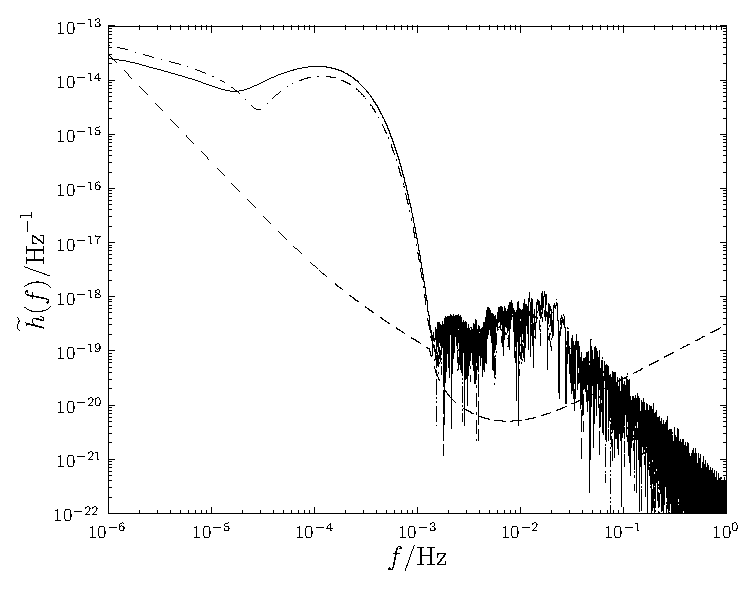
\includegraphics[width=0.47\textwidth]{./images/Fig_new_sph_h_233}} \quad
   \subfigure[{Waveform for $a_\ast \simeq 0.74$, $r\sub{p} \simeq 3.2 r\sub{g}$ and $\iota \simeq 1.2$. The SNR for the spherical polar kludge waveform (plotted) is $\rho[\boldsymbol{h}\sub{sph}] \simeq 70600$, for the oblate-spheroidal kludge it is $\rho[\boldsymbol{h}\sub{ob}] \simeq 74900$.}]{\label{fig:Orbit_135} 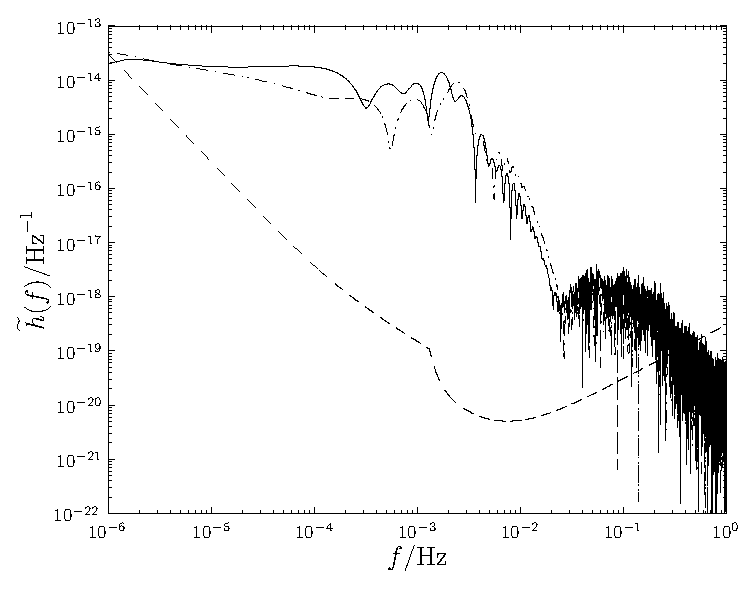
\includegraphics[width=0.47\textwidth]{./images/Fig_new_sph_h_135}}  
\caption{Example burst waveforms from the galactic centre. The strain $\widetilde{h}\sub{I}(f)$ is indicated by the solid line, $\widetilde{h}\sub{II}(f)$ by the dot--dashed line, and the noise curve by the dashed line. The kludge has been formulated using spherical polar coordinates.}
  \label{fig:Examples}
\end{figure}

The plotted waveforms use the spherical polar coordinate system for the NK. Using oblate-spheroidal coordinates makes a small difference. On the scale shown here the only discernible difference would be in \figref{Orbit_135}; the maximum difference in that waveform (outside the high-frequency tail) is $\sim 10\%$. In the other cases the difference is entirely negligible (except in the high-frequency tail, which is not of physical significance). This behaviour is typical; for the closest orbits, with the most extreme spin parameters, the maximum difference in the waveforms may be $\sim 30\%$. The difference is largely confined to the higher frequency components, which are most sensitive to the parts of the trajectory closer to the MBH: the change in flat-space radius for the same Boyer--Lindquist radial coordinate causes a slight shift in the shape of the spectrum. Enforcing the same flat-space periapsis gives worse agreement across the spectrum.

To examine the effect of the coordinate choice, we compare SNRs calculated using the alternative schemes for a selection of orbits. The orbits have periapse distances uniformly distributed in log-space between the innermost orbit and $100 r\sub{g}$. Each had a spin and orbital inclination randomly chosen from distributions uniform in $a_\ast$ and $\cos \iota$.\footnote{The innermost orbit depends upon $a_\ast$ and $\iota$, hence these are drawn first.} For every periapse, five SNRs were calculated, each having a different set of ancillary parameters specifying the relative orientation of the MBH, the orbital phase and the position of the detector, drawn from appropriate uniform distributions. We take the mean of $\ln \rho$ for each set of ancillary parameters.\footnote{The logarithm is a better quantity to work with since the SNR is a positive-definite quantity that may be distributed over a range of magnitudes \citep[sections 22.1, 23.3]{MacKay2003}. Using median values yields results that are quantitatively similar.} The MBH parameters were fixed as for the GC.

The ratio of the two SNRs is shown in \figref{Oblate_sphere}.
\begin{figure}%[!htp]
\centering
 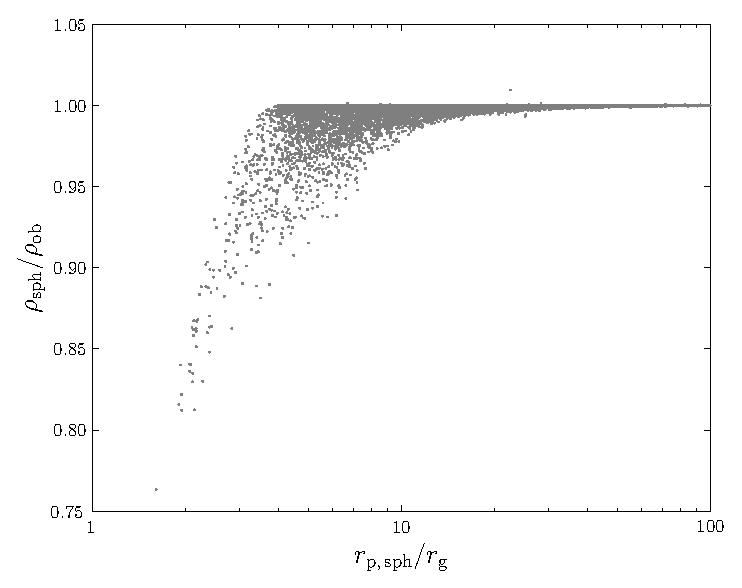
\includegraphics[width=0.6\textwidth]{./images/Fig_SNR_ratio}
 \caption{Ratio of SNR for a waveform calculated using spherical polar coordinates to that for a waveform using oblate-spheroidal coordinates.}
   \label{fig:Oblate_sphere}
\end{figure}
The difference from the coordinate systems is only apparent for orbits with very small periapses. There is agreement to $10\%$ down to $r\sub{p} \simeq 4 r\sub{g}$; the maximal difference may be expected to be $\sim 20\%$, this is for periapses that are only obtainable for high spin values.

Since the deviation in the two waveforms is only apparent for small periapses, when the kludge approximation is least applicable, we conclude that the choice of coordinates is unimportant. The potential error of order $10\%$ is no greater than that inherent in the NK approximation (see \secref{Energy}). Without an accurate waveform template to compare against, we do not know if there is a preferable choice of coordinates. We adopt spherical coordinates for easier comparison with existing work.

\subsection{Signal-to-noise ratios}\label{sec:Gal-SNR}

The detectability of a burst depends upon its SNR. To characterise the variation of $\rho$ we calculated SNRs for a range of orbits. These were generated as in \secref{wave-ex}, we used $\sim 10^4$ different periapse distances.

The bursts were calculated for a $1 M_\odot$ CO. From \eqnref{octupole}, the amplitude of the waveform is proportional to the CO mass $\mu$, and so $\rho$ is also proportional to $\mu$; a $10 M_\odot$ object would be ten times louder on the same orbit. To make results mass independent, we work in terms of a mass-normalised SNR
\begin{equation}
\hat{\rho}[\boldsymbol{h}] = \left(\dfrac{\mu}{M_\odot}\right)^{-1}\rho[\boldsymbol{h}].
\end{equation}

There exists a correlation between the periapse radius and SNR, as shown in \figref{SNR}.
\begin{figure}%[!htp]
  \centering
  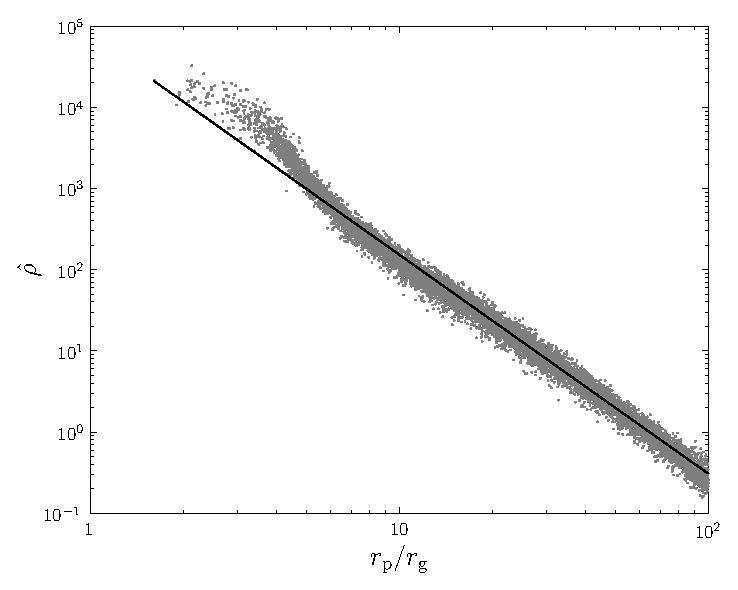
\includegraphics[width=0.6\textwidth]{./images/Fig_SNR}
    \caption{Mass-normalised SNR as a function of periapse radius for LISA. The plotted points are the values obtained by averaging over each set of ancillary parameters. The best fit line is $\log(\hat{\rho}) = -2.69\log(r\sub{p}/r\sub{g}) + 4.88$. This is fitted to orbits with $r\sub{p} >  13.0 r\sub{g}$.} % and has a reduced chi-squared value of $\chi^2/\nu = 1.73$
  \label{fig:SNR}
\end{figure}
Closer orbits produce louder bursts. To reflect this trend, we have fitted a simple fiducial power law,
\begin{equation}
\log\rho \simeq -2.7\log\left(\dfrac{r\sub{p}}{r\sub{g}}\right) + \log\left(\dfrac{\mu}{M_\odot}\right) + 4.9,
\label{eq:SNR-power-law}
\end{equation}
which is indicated by the straight line.\footnote{Using oblate-spheroidal coordinates instead of spherical polars gives a fit consistent to within $0.1\%$ as we have excluded the closest orbits.} This was done by maximising the likelihood, assuming $\ln \rho$ has a Gaussian distribution with standard deviation derived from the scatter because of variation in the ancillary parameters. The power law is a good fit only for larger periapses. The shape is predominately determined by the noise curve. The change in the trend reflects the transition from approximately power law behaviour to the bucket of the noise curve. Hence, we fit a power law to orbits with a characteristic frequency of $f_\ast = \sqrt{GM_\bullet/r\sub{p}} < 1 \times 10^{-3}\units{Hz}$, to avoid spilling into the bucket.\footnote{The form of $f_\ast$ can be derived on dimensional grounds, but it is explained in more detail in \secref{extragal-SNR}.} Changing the cut-off within a plausible region alters the fit coefficients by around $0.1$.\footnote{The power law exponent $-2.7$ is inconsistent with $-13/4$ as predicted by the approximate model of \citet{Hopman2007}. This is the result of their approximate waveform model.}

The SNR shows no clear correlation with the other parameters (excluding $\mu$). However, the SNR is sensitive to the orbital parameters, in particular the initial position, and may vary by an order of magnitude.

Setting a threshold of $\rho = 10$, a $1 M_\odot$ ($10 M_\odot$) object would be expected to be detectable if the periapse distance is less than $27 r\sub{g}$ ($65 r\sub{g}$). \citet{Hopman2007}, assuming a threshold of $\rho = 5$, used an approximate form for the SNR based upon the quadrupole component of a circular orbit; their model, with updated parameters for the MBH, predicts bursts would be detectable out to $66 r\sub{g}$ ($135 r\sub{g}$). This is overly optimistic.

Following a similar approach, we may repeat this analysis for eLISA. The SNR as a function of periapse is shown in \figref{SNR-eLISA}.
\begin{figure}%[!htp]
  \centering
  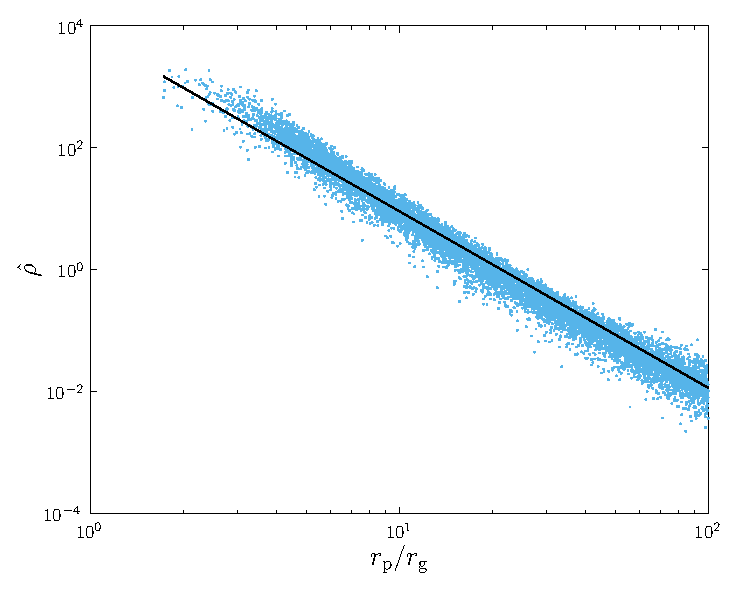
\includegraphics[width=0.6\textwidth]{./images/Fig_SNR_eLISA_NGO}
    \caption{Mass-normalised SNR as a function of periapse radius for eLISA. The plotted points are the values obtained by averaging over each set of ancillary parameters. The best fit line is $\log(\hat{\rho}) = -2.90\log(r\sub{p}/r\sub{g}) + 3.85$. This is fitted to orbits with $r\sub{p} >  13.0 r\sub{g}$.}
    \label{fig:SNR-eLISA}
\end{figure}
There is again a strong correlation that may be approximated as a power law. The bucket of the noise curve is less apparent as it is shifted to slightly higher frequencies. We have fitted
\begin{equation}
\log\rho \simeq -2.9\log\left(\dfrac{r\sub{p}}{r\sub{g}}\right) + \log\left(\dfrac{\mu}{M_\odot}\right) + 3.9,
\label{eq:SNR-power-law-eLISA}
\end{equation}
which is indicated by the straight line. This was done in exactly the same as for LISA. Again, there is no clear correlation with any other orbital parameters.

The SNR is lower for eLISA. As a consequence, bursts are detectable across a smaller range of periapses. Using the threshold $\rho = 10$, a $1 M_\odot$ ($10 M_\odot$) object would be expected to be detectable if the periapse distance is less than $10 r\sub{g}$ ($21 r\sub{g}$). This is a reduction of about a factor of three compared to LISA.

\section{Parameter estimation}\label{sec:Estimation}

Having detected a signal, we are interested in what we can learn about the source. We have an inference problem that can be solved by an application of Bayes' Theorem \citep[chapter 4]{Jaynes2003}: the probability distribution for our parameters given that we have detected the signal $\boldsymbol{s}(t)$ is given by the posterior
\begin{equation}
p(\boldsymbol{\lambda}|\boldsymbol{s}(t)) = \dfrac{p(\boldsymbol{s}(t)|\boldsymbol{\lambda})p(\boldsymbol{\lambda})}{p(\boldsymbol{s}(t))}.
\end{equation}
Here $p(\boldsymbol{s}(t)|\boldsymbol{\lambda})$ is the likelihood of the parameters, $p(\boldsymbol{\lambda})$ is the prior probability distribution for the parameters, and the evidence $p(\boldsymbol{s}(t)) = \intd{}{}{p(\boldsymbol{s}(t)|\boldsymbol{\lambda})}{^d \lambda}$ is, for our purposes, a normalising constant. The likelihood depends upon the realization of noise. If parameters $\boldsymbol{\lambda}_0$ define a waveform $\boldsymbol{h}_0(t) = \boldsymbol{h}(t; \boldsymbol{\lambda}_0)$, the probability that we observe signal $\boldsymbol{s}(t)$ GW is given by \eqnref{sig_prob}, so the likelihood is
\begin{equation}
p(\boldsymbol{s}(t)|\boldsymbol{\lambda}_0) \propto \exp\left[-\recip{2}\innerprod{\boldsymbol{s}-\boldsymbol{h}_0}{\boldsymbol{s}-\boldsymbol{h}_0}\right].
\label{eq:likelihood}
\end{equation}
If we were to define this as a probability distribution for the parameters $\boldsymbol{\lambda}$, the modal values are the maximum-likelihood (ML) parameters $\boldsymbol{\lambda}\sub{ML}$. The waveform $\boldsymbol{h}(t; \boldsymbol{\lambda}\sub{ML})$ is the signal closest to $\boldsymbol{s}(t)$, where distance is defined using the inner product (\ref{eq:inner}) \citep{Cutler1994}.

To discover if any parameters can be accurately inferred, we must characterise the form of the posterior. We discuss two approaches for mapping the shape of the posterior: Fisher matrices and Markov chain Monte Carlo (MCMC) sampling.

\subsection{Fisher matrices}\label{sec:Fisher}

In the limit of a high SNR, we may approximate \citep{Vallisneri2008}
\begin{equation}
p(\boldsymbol{s}(t)|\boldsymbol{\lambda}_0) \propto \exp\left[-\recip{2}\innerprod{\partial_a\boldsymbol{h}}{\partial_b\boldsymbol{h}}\left(\lambda^a - \langle\lambda^a\rangle_\ell\right)\left(\lambda^b - \left\langle\lambda^b\right\rangle_\ell\right)\right],
\label{eq:LSA}
\end{equation}
where the mean is defined as
\begin{equation}
\langle\lambda^a\rangle_\ell = \dfrac{\intd{}{}{\lambda^a p(\boldsymbol{s}(t)|\boldsymbol{\lambda})}{^d \lambda}}{\intd{}{}{p(\boldsymbol{s}(t)|\boldsymbol{\lambda})}{^d \lambda}}.
\end{equation}
In the high SNR limit, this is the ML value $\langle\lambda^a\rangle_\ell = \lambda^a\sub{ML}$. The quantity
\begin{equation}
\Gamma_{ab} = \innerprod{\partial_a\boldsymbol{h}}{\partial_b\boldsymbol{h}}
\label{eq:Fisher}
\end{equation}
is the Fisher information matrix (FIM). It controls the variance of the likelihood distribution.

The form of the posterior distribution depends upon the nature of the prior information. If we have an uninformative prior, such that $p(\boldsymbol{\lambda})$ is a constant, the posterior distribution is determined by the likelihood. In the high SNR limit, we obtain a Gaussian with variance-covariance matrix
\begin{equation}
\boldsymbol{\Sigma} = \boldsymbol{\Gamma}^{-1}.
\label{eq:InvFisher}
\end{equation}
The FIM therefore gives the uncertainty associated with the inferred parameters, in this case the ML values.

If the prior restricts the allowed range for a parameter, as is the case for the spin $a_\ast$, then the posterior is a truncated Gaussian, and $\boldsymbol{\Gamma}^{-1}$ may no longer represent the variance-covariance.

If the prior is approximately Gaussian with variance-covariance matrix $\boldsymbol{\Sigma}_0$, the posterior is also Gaussian.\footnote{If we only know the typical value and spread of a parameter, a Gaussian is the maximum entropy prior (\citealt{Jaynes2003}, section 7.11): the prior that is least informative given what we know.} The posterior variance-covariance is \citep{Cutler1994, Vallisneri2008}
\begin{equation}
\boldsymbol{\Sigma} = \left(\boldsymbol{\Gamma} + \boldsymbol{\Sigma}_0^{-1}\right)^{-1}.
\label{eq:Posterior_variance}
\end{equation}
From this the inverse FIM $\boldsymbol{\Gamma}^{-1}$ is an upper bound on the size of the posterior covariance matrix.\footnote{It is also the Cram\'{e}r-Rao bound on the error covariance of an unbiased estimator \citep{Cutler1994, Vallisneri2008}. Thus it represents the frequentist error: the lower bound on the covariance for an unbiased parameter estimator $\boldsymbol{\lambda}\sub{est}$ calculated from an infinite set of experiments with the same signal $\boldsymbol{h}(t)$ but different realisations of the noise $\boldsymbol{n}(t)$.}

The FIM gives a quick way of estimating the range of the posterior. It is widely used because of this. However, it is only appropriate when the approximation of \eqnref{LSA} holds. This is known as the linearised-signal approximation (LSA), where higher order derivatives are neglected. To assess the validity of this, \citet{Vallisneri2008} recommends use of the maximum-mismatch (MM) criterion
\begin{equation}
\ln r = -\recip{2}\innerprod{\Delta\lambda^a\partial_a\boldsymbol{h}\sub{ML} - \Delta\boldsymbol{h}}{\Delta\lambda^b\partial_b\boldsymbol{h}\sub{ML} - \Delta\boldsymbol{h}}.
\end{equation}
Here $\Delta \boldsymbol{\lambda}$ is the displacement to some point on the $1\sigma$ surface
\begin{equation}
\Delta \boldsymbol{\lambda} = \boldsymbol{\lambda}\sub{1\sigma} - \boldsymbol{\lambda}\sub{ML},
\end{equation}
and $\Delta \boldsymbol{h}$ is the corresponding change in the waveform
\begin{equation}
\Delta \boldsymbol{h} = \boldsymbol{h}(\boldsymbol{\lambda}\sub{1\sigma}) - \boldsymbol{h}(\boldsymbol{\lambda}\sub{ML}).
\end{equation}
The $1\sigma$ surface is defined from the inverse of the FIM. If higher order terms are indeed negligible, the MM criterion is small. We check this by picking a random selection of points on the $1\sigma$ surface and evaluating $|\ln r|$. If this is smaller than a fiducial value ($|\ln r| = 0.1$) over the majority ($90\%$) of the surface we consider the LSA sufficiently justified.

We calculated FIMs for a wide range of orbits and checked the MM criterion. We found that for the overwhelming majority the test failed: the LSA is not appropriate. This behaviour was seen even for orbits with $\rho \sim 10^3$--$10^4$.\footnote{In this study, to increase $\rho$ we must reduce the periapse distance; this also reduces the region where the LSA is valid as parameter dependencies become more non-linear. If we had the luxury of increasing $\rho$ by moving the GC closer, things could be different.} Higher order terms are important, and cannot be neglected.

EMRBs have a short duration and accordingly are not the most informative of signals. Therefore, the $1\sigma$ surface as defined by considering only the LSA terms is large. Taking such a step in parameter space moves the signal beyond the region of linear changes.

What constitutes high SNR depends upon the signal; it is not enough for $\rho > 1$. As stressed by \citet{Vallisneri2008}, it is essential to check the MM criterion for individual waveforms: the threshold for the LSA to become applicable could be much greater than naively thought.

As we cannot be confident in FIM results, we abandon this approach in favour of using Markov chain Monte Carlo simulations to explore constraints from different regions of parameter space. These are computationally more expensive, but do not rely on any approximations.

\subsection{Markov chain Monte Carlo methods}\label{sec:MCMC}

MCMC methods are widely used for inference problems; they are a family of algorithms for integrating over complicated distributions and are efficient for high-dimensional problems \citep[chapter 29]{MacKay2003}. Parameter space is explored by constructing a chain of $N$ samples. The distribution of points visited by the chain maps out the underlying distribution; this becomes asymptotically exact as $N \rightarrow \infty$. Samples are added sequentially, if the current state is $\boldsymbol{\lambda}_n$ a new point $\boldsymbol{\lambda}^\ast$ is drawn and accepted with probability
\begin{equation}
\mathcal{A} = \min\left\{\dfrac{\pi(\boldsymbol{\lambda}^\ast)\mathcal{L}(\boldsymbol{\lambda}^\ast)\mathcal{Q}(\boldsymbol{\lambda}_n;\,\boldsymbol{\lambda}^\ast)}{\pi(\boldsymbol{\lambda}_n)\mathcal{L}(\boldsymbol{\lambda}_n)\mathcal{Q}(\boldsymbol{\lambda}_n;\,\boldsymbol{\lambda}^\ast)}, 1\right\},
\end{equation}
setting $\boldsymbol{\lambda}_{n + 1} = \boldsymbol{\lambda}^\ast$, where $\mathcal{L}(\boldsymbol{\lambda})$ is the likelihood, in our case from \eqnref{likelihood}; $\pi(\boldsymbol{\lambda})$ is the prior, and $\mathcal{Q}$ is a proposal distribution. If the move is not accepted  $\boldsymbol{\lambda}_{n + 1} = \boldsymbol{\lambda}_n$. This is the Metropolis-Hastings algorithm \citep{Metropolis1953,Hastings1970}.

Waiting long enough yields an exact posterior, but it is desirable for the MCMC to converge quickly. This requires a suitable choice for the proposal distribution, which can be difficult, since we do not yet know the shape of the target distribution.

One method to define the proposal is to use the previous results in the chain and refine $\mathcal{Q}$ by learning from these. Such approaches are known as adaptive methods. Updating using previous points means that the chain is no longer Markovian. Care must be taken to ensure that ergodicity is preserved and convergence obtained \citep{Roberts2007,Andrieu2008}. To avoid this complication, we follow \citet{Haario1999}, and use the adapting method as a burn in phase. We have an initial phase where the proposal is updated based upon accepted points. After this we fix the proposal and proceed as for a standard MCMC. By only using samples from the second part, we guarantee that the chain is Markovian and ergodic, whilst still enjoying the benefits of a tailor-made proposal. After only a finite number of samples we cannot assess the optimality of this \citep{Andrieu2008}, but the method is still effective.

To tune $\mathcal{Q}$, we use an approach based upon the adaptive Metropolis algorithm \citep{Haario2001}. The proposal is taken to be a multivariate normal distribution centred upon the current point, the covariance of which is
\begin{equation}
\boldsymbol{C} = s \left(\boldsymbol{V}_n + \varepsilon\boldsymbol{C}_0\right),
\end{equation}
where $\boldsymbol{V}_n$ is the covariance of the accepted points $\{\boldsymbol{\lambda}_1,\ldots,\boldsymbol{\lambda}_n\}$, $s$ is a scaling factor that controls the step size, $\varepsilon$ is a small positive constant (typically $2.5 \times 10^{-3}$), and $\boldsymbol{C}_0$ is a constant matrix included to ensure ergodicity.

Our adaptation is run in three phases. The initial phase is to get the chain moving. For this $\boldsymbol{C}_0\super{init}$ is a diagonal matrix with elements calibrated from initial one dimensional MCMCs. This finishes after $N\sub{init}$ accepted points.

For the second phase, we use the proposal covariance from the initial phase $\boldsymbol{C}\super{init}$ for $\boldsymbol{C}_0\super{main}$. We reset the covariance of the accepted points so that it only includes points from this phase. This is the main adaptation phase and lasts until $N\sub{main}$ points have been accepted.

In the final adaptation phase we restart the chain at the true parameter values. We no longer update the shape of the covariance ($\boldsymbol{V}_n$ remains fixed), but adjust the step size $s$ to tune the acceptance rate; it is then fixed, along with everything else, for the final MCMC.

Throughout the adaptation, we update the step size $s$ after every $100$ trial points (whether or not they are accepted). While updating, the covariance $\boldsymbol{V}_n$ changes after every $10^3$ trial points. We set $N\sub{init} = 5 \times 10^4$ and $N\sub{main} = 4.5 \times 10^5$.

We initially aimed for an acceptance rate of $0.234$; this is optimal for a random walk Metropolis algorithm with some specific high-dimensional target distributions \citep{Roberts1997,Roberts2001}. In many cases we found better convergence when aiming for a lower acceptance rate, say $0.1$. This is not unexpected: the optimal rate may be lower than $0.234$ when the parameters are not independent and identically distributed \citep{Bedard2007, Bedard2008, Bedard2008a}. In practice, the final acceptance rate is (almost always) lower than the target rate as the use of a multivariate Gaussian for the proposal distribution is rarely a good fit at the edges of the posterior. Consequently, the precise choice for the target acceptance rate is unimportant as long as it is of the correct magnitude. Final rates are typically within a factor of $2$ of the target value. As an initial choice, we set $s = 2.38^2/d$, which is the optimal choice if $\boldsymbol{C}$ was the true target covariance for a high dimensional target of independent and identically distributed parameters \citep{Gelman1996,Roberts1997,Roberts2001,Haario2001}.\footnote{Reasonably good results may be obtained by fixing $s$ at this value, and not adjusting to fine tune the acceptance rate.}

To assess the convergence of the MCMC we check the trace plot (the parameters' values throughout the run) for proper mixing, that the one and two dimensional posterior plots fill out to a smooth distribution, and that the distribution widths tend towards consistent values.

\section{Results for Galactic bursts}\label{sec:Gal-Results}

To asses the utility of EMRBs for parameter estimation, we studied bursts from a range of orbits with periapses uniformly distributed in logarithmic space between the the inner-most orbit and $16 r\sub{g}$. Parameters were chosen as in \secref{wave-ex}. The MBH was assumed to have the standard mass and position and the CO was chosen to be $10 M_\odot$, as the most promising candidates for EMRBs would be BHs: they are massive and hence produce higher SNR bursts, they are more likely to be on close orbits as a consequence of mass segregation \citep{Bahcall1977, Alexander2009}, and they cannot be tidally disrupted.

The results of the MCMC runs show strong and complex parameter dependencies. Some example results are shown in \figref{MCMC-1}, \ref{fig:MCMC-2} and \ref{fig:MCMC-3}.
\begin{figure}%[!htp]
\centering
\vspace{0.5\baselineskip}
   \includegraphics[width=0.8\textwidth]{./images/Fig_MCMC_327_triangle_40}
\caption{Marginalised one- and two-dimensional posteriors. The scales are identical in both sets of plots. The dotted line indicates the true value. These distributions are fairly cromulent and well converged. Angular momentum is in units of $L_\bullet = GM_\bullet c^{-1}$  and the scaled distance is in units of $\zeta_0 = 1 M_\odot^{-1}\units{kpc}$. The input orbit has $r\sub{p} \simeq 8.54 r\sub{g}$ and $\rho \simeq 916$.}
\label{fig:MCMC-1}
\end{figure}
The first is well-behaved. It is almost Gaussian, but we see some asymmetries and imperfections. There are also strong degeneracies, indicated by needle-like distributions. This is a fairly standard example: there are runs which are closer to being Gaussian (especially at higher SNR), and equally there are tighter correlations. The lenticular $M_\bullet$--$L_\infty$ degeneracy is common.

\begin{figure}%[!htp]
\centering
\vspace{0.5\baselineskip}
   \includegraphics[width=0.8\textwidth]{./images/Fig_MCMC_53_triangle_40}
\caption{Marginalised one- and two-dimensional posteriors. The conventions are the same as in \figref{MCMC-1}. These distributions show definite non-gaussianity. The input orbit has $r\sub{p} \simeq 9.86 r\sub{g}$ and $\rho \simeq 1790$.}
\label{fig:MCMC-2}
\end{figure}
The second shows banana-like degeneracies. These are not uncommon; there are varying degrees of curvature. The more complicated shape makes it harder for the MCMC to converge, so the final distribution is not as smooth as for the first example. The curving degeneracies also bias the one dimensional marginalisations away from the true values.

\begin{figure}%[!htp]
\centering
\vspace{0.5\baselineskip}
   \includegraphics[width=0.8\textwidth]{./images/Fig_MCMC_181_triangle_40}
\caption{Marginalised one- and two-dimensional posteriors. The conventions are the same as in \figref{MCMC-1}. These distributions show complicated degeneracies. The input orbit has $r\sub{p} \simeq 11.60 r\sub{g}$ and $\rho \simeq 590$.}
\label{fig:MCMC-3}
\end{figure}
The third shows more intricate behaviour. This is more rare, but indicates the variety of shapes that is obtainable. Again the convergence is more difficult, so the distributions are rougher around the edges; there is also some biasing due to the curving degeneracies.

Our results do not incorporate any priors (save to keep them within realistic ranges); we have not folded in the existing information we have, for example, about the MBH's mass. Therefore, the resulting distributions characterise what we could learn from EMRBs alone. By the time a space-borne GW detector finally flies, we will have much better constraints on some parameters.

It is possible to place good constraints from the closest orbits. These can provide sufficient information to give beautifully behaved posteriors although significant correlation between parameters persists.

\subsection{Distribution widths}

\subsubsection{Characterising distributions}\label{sec:k-d}

Having recovered the posterior distribution it is necessary to quantify the accuracy to which parameters could be measured. If the posterior were Gaussian, this can be done just by using the standard deviation $\sigma\sub{SD}$. An alternative is to use the range that encloses a given probability, but this is misleading if the distribution is multimodal. A robust means of characterising the width is by using a $k$-dimensional ($k$-d) tree.

A $k$-d tree is a type of binary space partitioning tree \citep[sections 5.2, 12.1, 12.3]{Berg2008}. It is constructed by splitting the parameter space into two by finding the median point in one dimension. The two pieces are then split by finding their medians in another dimension. This continues recursively until the desired number of partitions, known as leaves, has been created. When applied to a sampled probability distribution, a $k$-d tree has smaller leaves in the regions of high probability which are of most interest \citep{Weinberg2012}. It builds a natural decomposition of the parameter space, giving a means of binning samples.

For a given probability $p$, the corresponding confidence region is the smallest area of parameter space in which we expect that the true values lie with that probability. A simple means of constructing a confidence range is to find the smallest combination of $k$-d tree leaves that contain the desired probability. To do this we rank the leaves by size; the smallest corresponds to the highest probability area and is the starting point for the confidence range. We continue adding the next smallest leaf until the total probability enclosed is $p$. Summing the areas of the leaves gives an estimate for the range.

However, this approach is biased. Whenever a random fluctuation in the sampling gives an excess of points in one area the overdensity leads to a smaller leaf size and then the preferential inclusion of that leaf in the confidence interval. Conversely, an underdensity leads to a larger leaf that is liable to be external to the confidence range. If there are a small number of points per leaf we shall overstate our confidence as the constructed range is too small.\footnote{This can be visualised by considering the simple example of dividing in two samples from a one dimensional uniform distribution. We would expect one partition to be more densely populated than the other because of random fluctuations, and we shall always pick this smaller leaf as our $p = 0.5$ confidence range. As the number of points increases we expect that this bias would decrease.}

Biasing may be avoided by using a two-step method which separates the creation and ordering of the partitions from the building of the confidence range \citep{Sidery2013}. This is done by dividing our data into two disjoint random samples.\footnote{We split our data into two equal parts. This may not be the optimal rationing, but is a sensible first guess. Some preliminary experimentation shows that it is not too important, provided that the splitting is not too unbalanced. The point at which this occurs depends upon the underlying distribution.} The first is used to construct the $k$-d tree in the standard way. The leaves are then ordered by size. We then use the second set to populate the leaves. We again start with the smallest leaf and work down the ranking until the encompassed probability is $p$. The total range is the estimate for the $p$ confidence level.

The first step creates bins that are of appropriate resolution. We therefore have the benefit of using a $k$-d tree. By using an independent set of points to build the confidence level, we eliminate any bias because there should be no correlation in fluctuations between the two sets. Any leaves that are too small are expected to receive a below average number of points in the second step and any that are too large are expected to receive more. This corrects the expectation for the confidence level.

In this case, we are interested in the confidence levels for the marginalised distributions for each parameter. We therefore construct $1$-d trees, which are easily implemented. We have a large number of points and low dimensionality so biasing should not be an issue. To characterise our distributions we find the $p = 0.68$ confidence range and take the half-width of this, which we denote as $\sigma_{0.68}$.

\subsubsection{Parameter uncertainties}

Characteristic distribution widths $\sigma\sub{SD}$ and $\sigma_{0.68}$ are shown in \figref{sigmas}. Filled circles are used for runs that appear to have converged. Open circles are for those yet to converge, but which appear to be approaching an equilibrium state; widths should be accurate to within a factor of a few.
\begin{figure}%[!htp]
\centering
\subfigure[MBH mass $M_\bullet$ versus periapsis.]{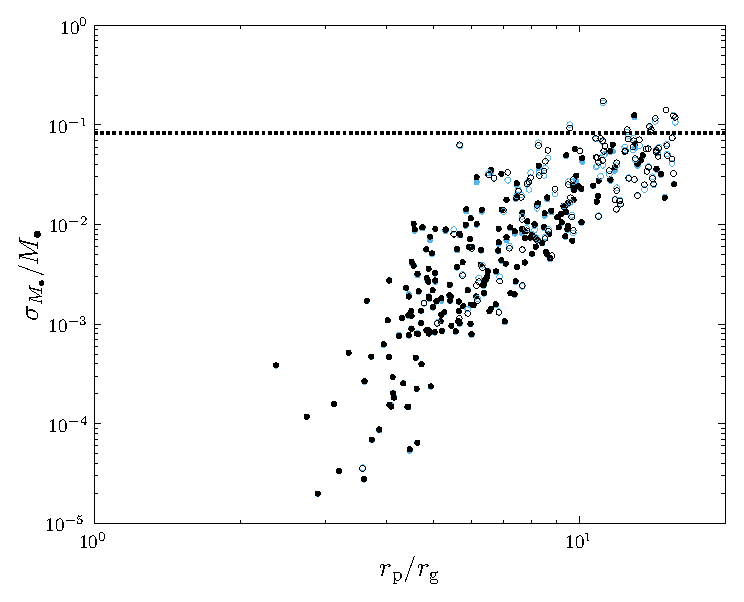
\includegraphics[width=0.475\textwidth]{./images/Fig_MW_MCMC_sigmas_rp_1}} \quad
\subfigure[MBH mass $M_\bullet$ versus SNR.]{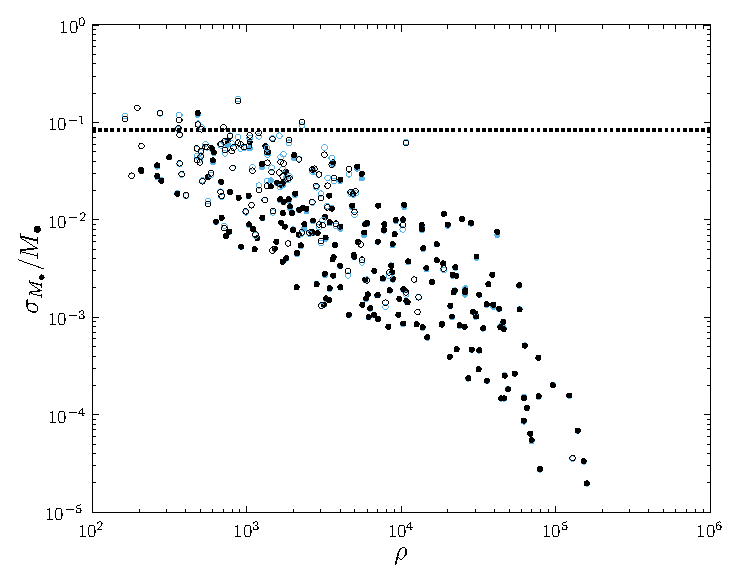
\includegraphics[width=0.485\textwidth]{./images/Fig_MW_MCMC_sigmas_SNR_1}} \\
\subfigure[MBH spin $a_\ast$ versus periapsis.]{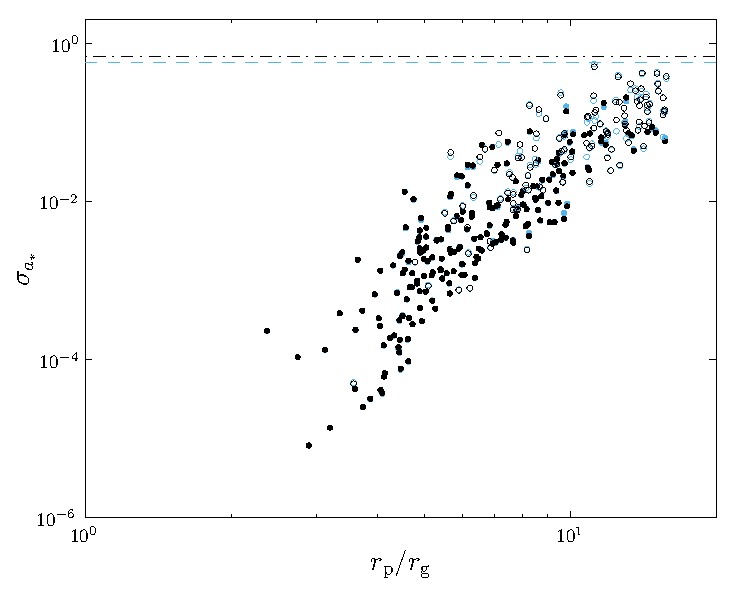
\includegraphics[width=0.475\textwidth]{./images/Fig_MW_MCMC_sigmas_rp_2}} \quad
\subfigure[MBH spin $a_\ast$ versus SNR.]{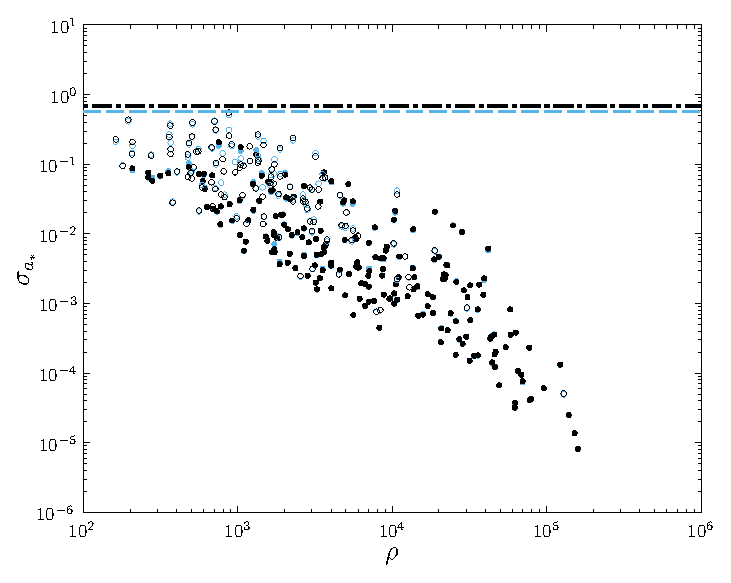
\includegraphics[width=0.485\textwidth]{./images/Fig_MW_MCMC_sigmas_SNR_2}} \\
\subfigure[Orientation angle $\Theta\sub{K}$ versus periapsis.]{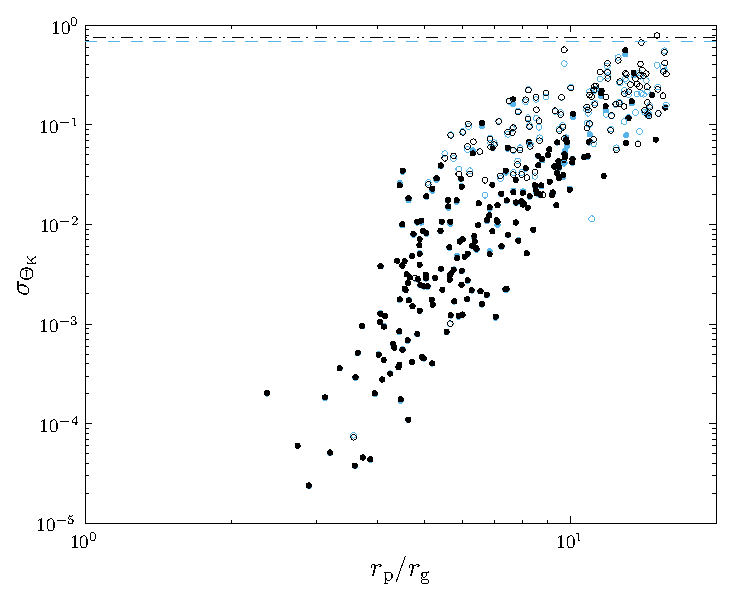
\includegraphics[width=0.475\textwidth]{./images/Fig_MW_MCMC_sigmas_rp_8}} \quad
\subfigure[Orientation angle $\Theta\sub{K}$ versus SNR.]{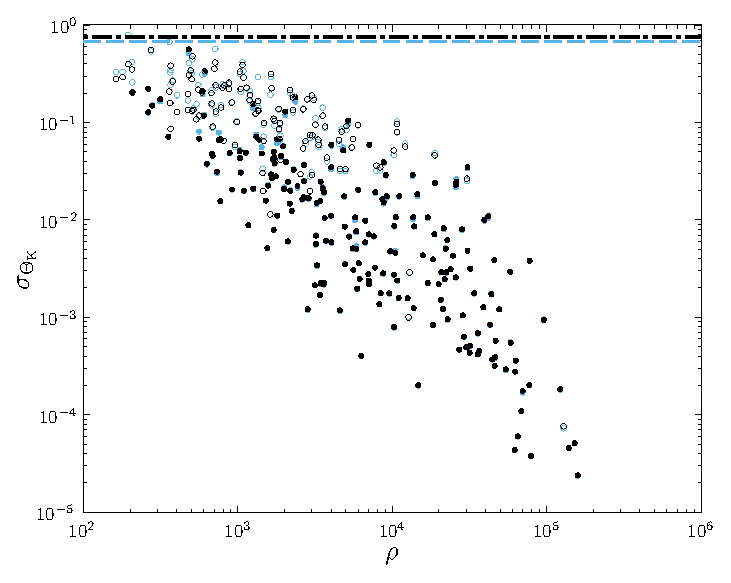
\includegraphics[width=0.485\textwidth]{./images/Fig_MW_MCMC_sigmas_SNR_8}}
\caption{Distribution widths as functions of periapsis $r\sub{p}$ and SNR $\rho$. The light blue points are used for the standard deviation, the black for the $68$-percentile half-width. The filled circles are converged runs and the open circles for those yet to converge. The dotted line is the current uncertainty for $M_\bullet$. The dashed line is the standard deviation for an uninformative prior and the dot--dashed line is the equivalent $68$-percentile half-width.}
\label{fig:sigmas}
\end{figure}
\begin{figure}%[!htp]
\setcounter{subfigure}{6}
\centering
\subfigure[Orientation angle $\Phi\sub{K}$ versus periapsis.]{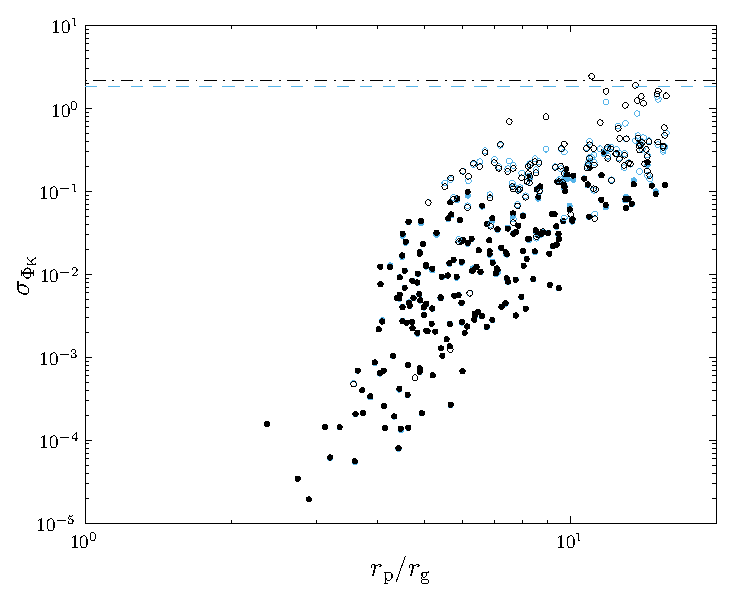
\includegraphics[width=0.475\textwidth]{./images/Fig_MW_MCMC_sigmas_rp_9}} \quad
\subfigure[Orientation angle $\Phi\sub{K}$ versus SNR.]{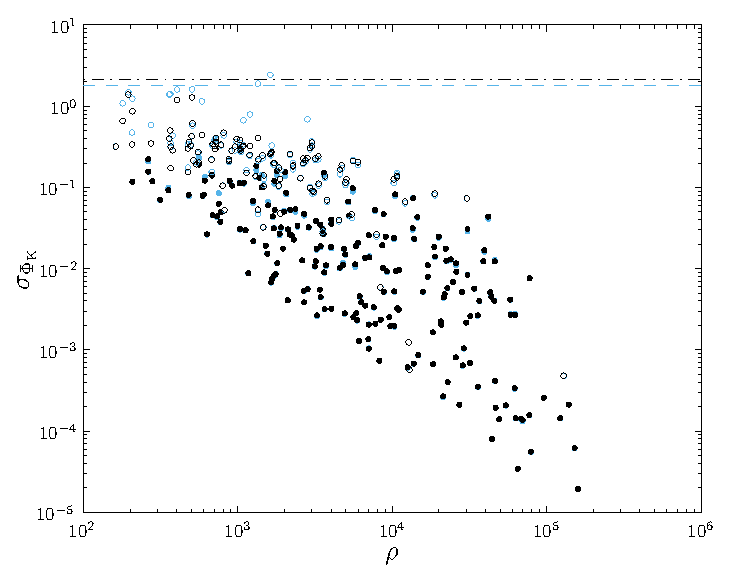
\includegraphics[width=0.485\textwidth]{./images/Fig_MW_MCMC_sigmas_SNR_9}} \\
\subfigure[Scaled distance $\zeta$ versus periapsis.]{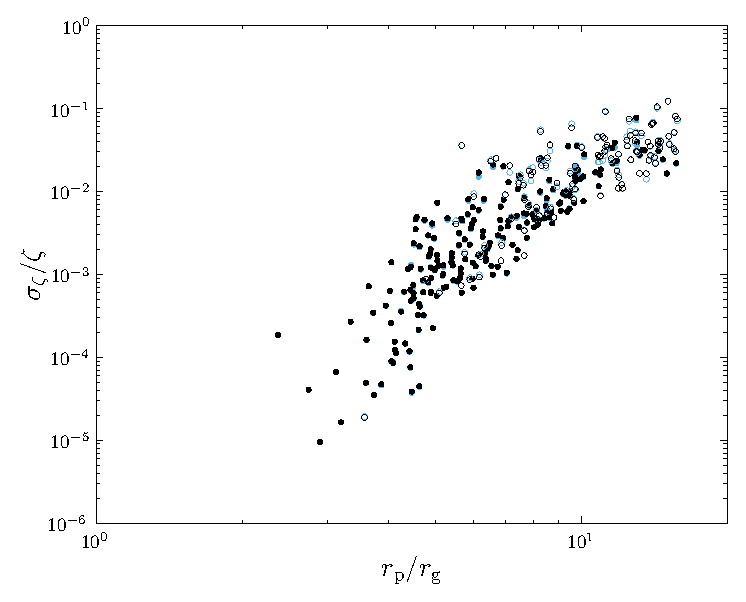
\includegraphics[width=0.475\textwidth]{./images/Fig_MW_MCMC_sigmas_rp_10}} \quad
\subfigure[Scaled distance $\zeta$ versus SNR.]{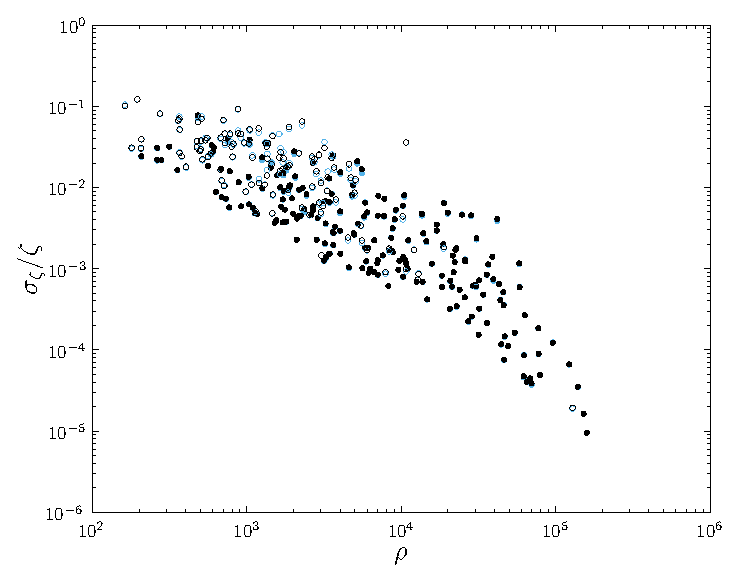
\includegraphics[width=0.485\textwidth]{./images/Fig_MW_MCMC_sigmas_SNR_10}} \\
\subfigure[Angular momentum $L_\infty$ versus periapsis.]{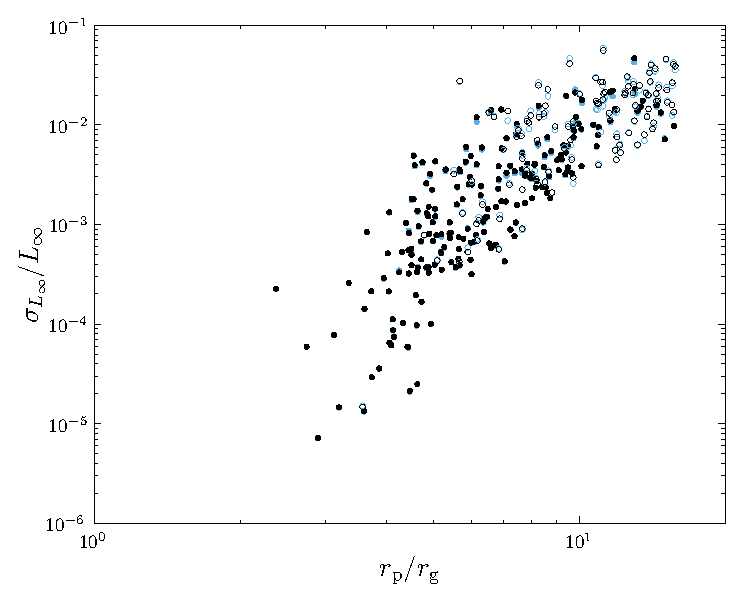
\includegraphics[width=0.475\textwidth]{./images/Fig_MW_MCMC_sigmas_rp_3}} \quad
\subfigure[Angular momentum $L_\infty$ versus SNR.]{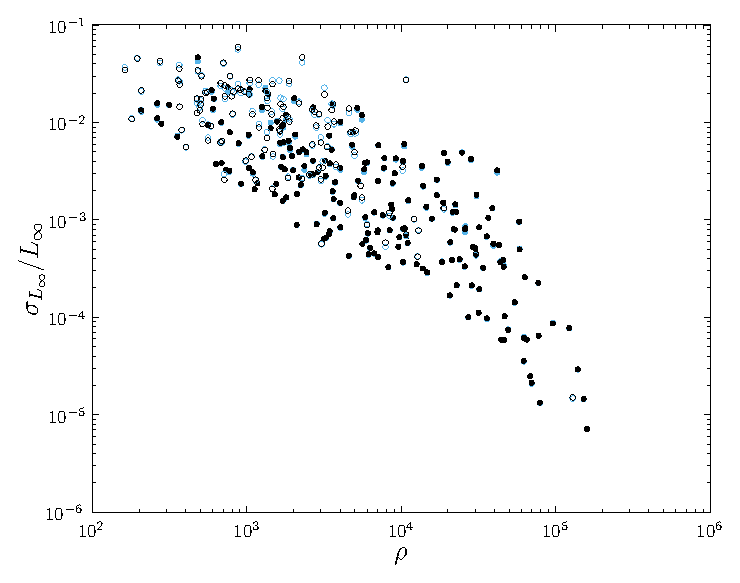
\includegraphics[width=0.485\textwidth]{./images/Fig_MW_MCMC_sigmas_SNR_3}} \\
\contcaption{{\bf{(Continued)}} Distribution widths as functions of periapse $r\sub{p}$ and SNR $\rho$.}
\end{figure}
\begin{figure}%[!htp]
\setcounter{subfigure}{12}
\centering
\subfigure[Orbital inclination $\iota$ versus periapsis.]{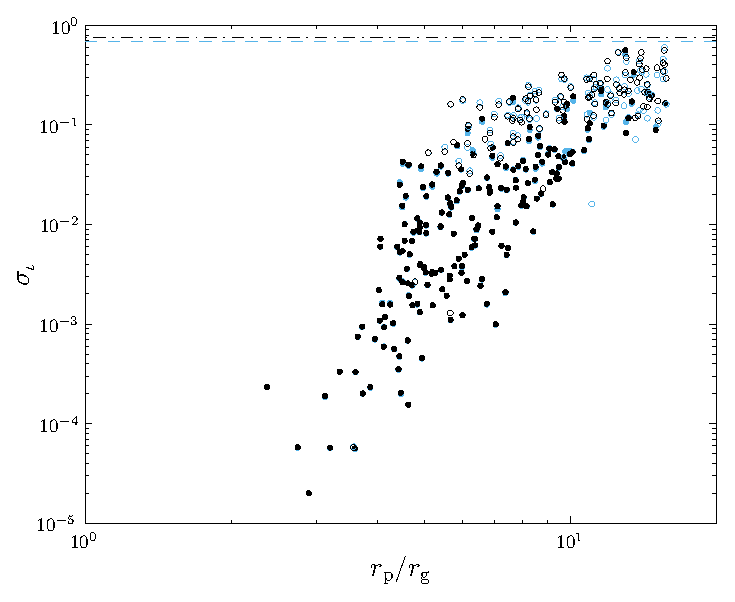
\includegraphics[width=0.475\textwidth]{./images/Fig_MW_MCMC_sigmas_rp_4}} \quad
\subfigure[Orbital inclination $\iota$ versus SNR.]{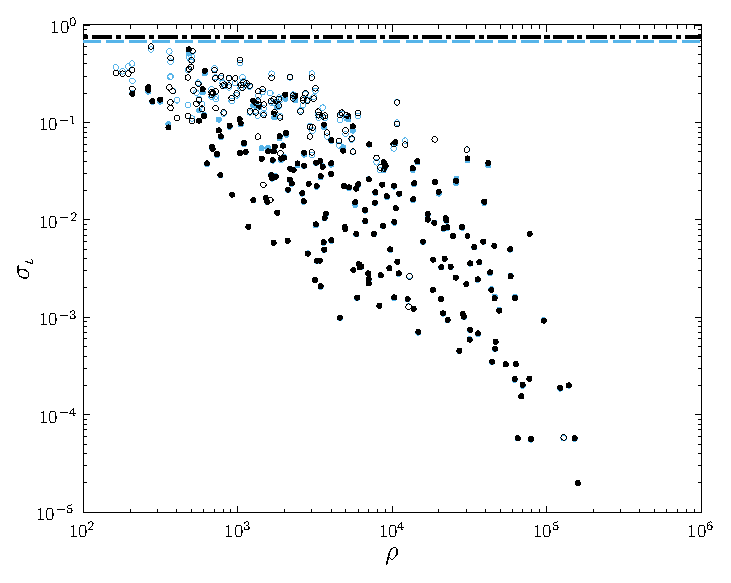
\includegraphics[width=0.485\textwidth]{./images/Fig_MW_MCMC_sigmas_SNR_4}} \\
\subfigure[Periapse azimuthal phase $\phi\sub{p}$ versus periapsis.]{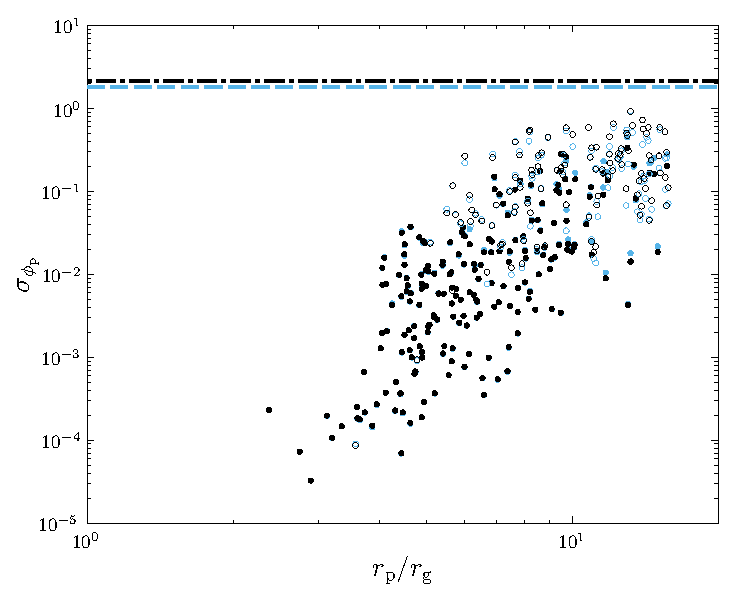
\includegraphics[width=0.475\textwidth]{./images/Fig_MW_MCMC_sigmas_rp_7}} \quad
\subfigure[Periapse azimuthal phase $\phi\sub{p}$ versus SNR.]{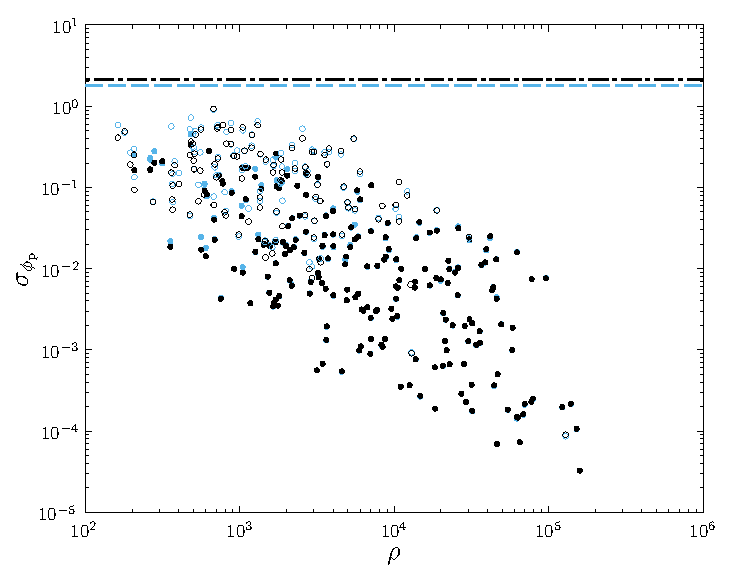
\includegraphics[width=0.485\textwidth]{./images/Fig_MW_MCMC_sigmas_SNR_7}} \\
\subfigure[Periapse polar phase $\chi\sub{p}$ versus periapsis.]{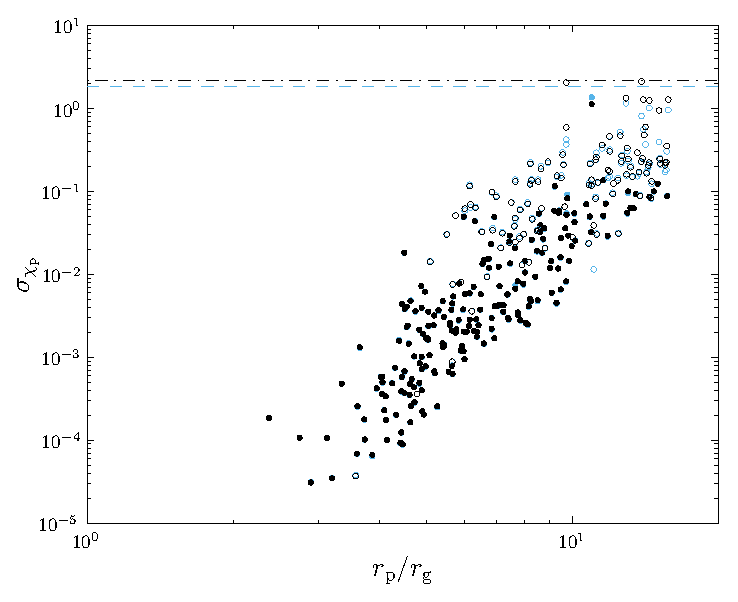
\includegraphics[width=0.475\textwidth]{./images/Fig_MW_MCMC_sigmas_rp_5}} \quad
\subfigure[Periapse polar phase $\chi\sub{p}$ versus SNR.]{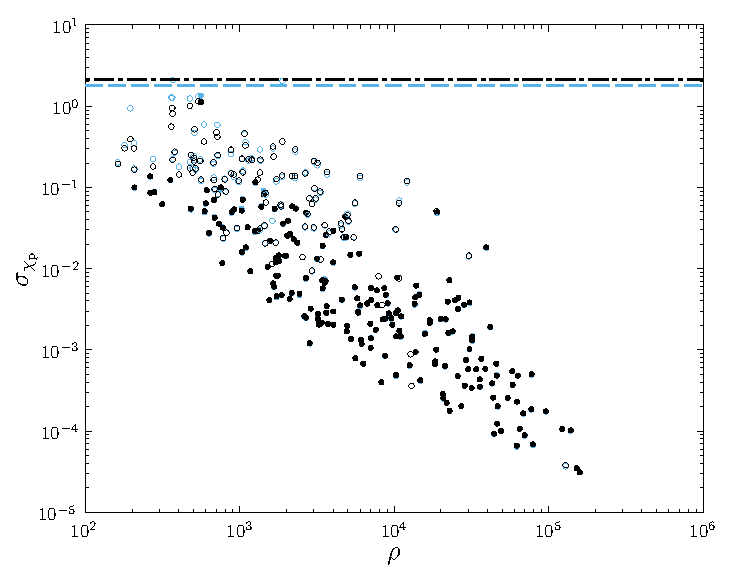
\includegraphics[width=0.485\textwidth]{./images/Fig_MW_MCMC_sigmas_SNR_5}} \\
\contcaption{{\bf{(Continued)}} Distribution widths as functions of periapse $r\sub{p}$ and SNR $\rho$.}
\end{figure}
\begin{figure}%[!htp]
\setcounter{subfigure}{18}
\centering
\subfigure[Periapse time $t\sub{p}$ versus periapsis.]{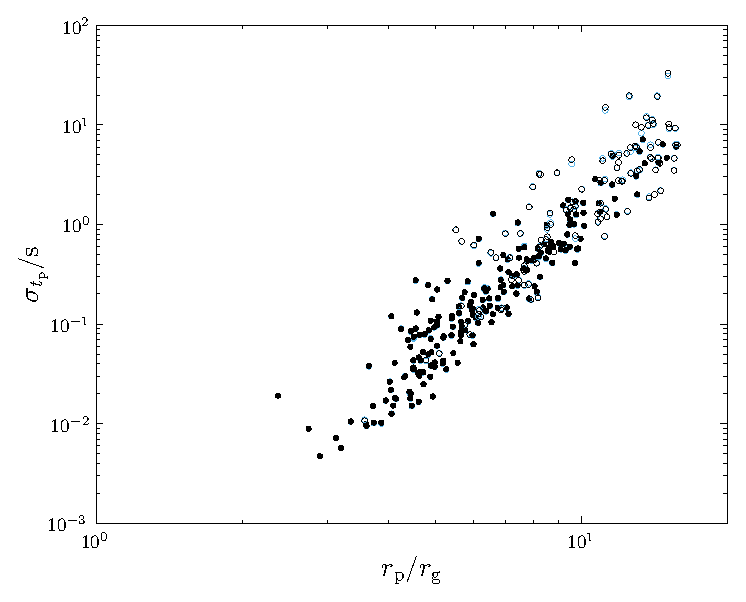
\includegraphics[width=0.475\textwidth]{./images/Fig_MW_MCMC_sigmas_rp_6}} \quad
\subfigure[Periapse time $t\sub{p}$ versus SNR.]{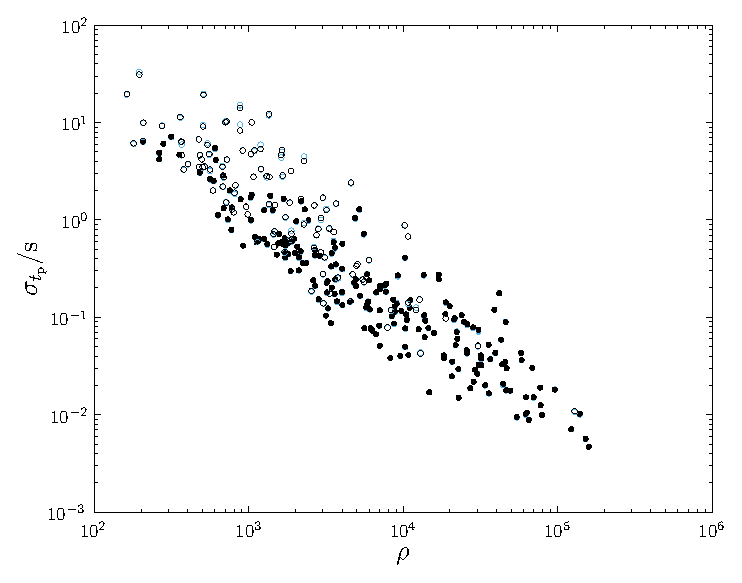
\includegraphics[width=0.485\textwidth]{./images/Fig_MW_MCMC_sigmas_SNR_6}} \\
\contcaption{{\bf{(Concluded)}} Distribution widths as functions of periapsis $r\sub{p}$ and SNR $\rho$.}
\setcounter{subfigure}{0}
\end{figure}
For guidance, the dotted line corresponds to the current measurement uncertainty for $M_\bullet$; the dashed lines are $\sigma\sub{SD}$ from uniform priors for $a_\ast$, $\Phi\sub{K}$, $\phi\sub{p}$, $\chi\sub{p}$, $\cos\Theta\sub{K}$ and $\cos\iota$, and the dot--dashed lines are the equivalent $\sigma_{0.68}$. We have no expectations for the width of the MBH mass distribution with respect to the current value. However, we would expect that the recovered distributions for the other parameters are narrower than for the case of complete ignorance; this bound does seem to be respected. The two widths, $\sigma\sub{SD}$ and $\sigma_{0.68}$, typically agree better at smaller periapses and higher SNRs as would be expected for more Gaussian distributions.

The widths show a trend of decreasing with decreasing periapsis or increasing SNR, but there is a large degree of scatter. There does not appear to be a strong dependence upon any single input parameter, with the exception of the spin. The widths for $\iota$, $\Theta\sub{K}$, $\Phi\sub{K}$, $\phi\sub{p}$ and $\chi\sub{p}$ increase for smaller spin magnitudes. The dependence is shown in \figref{sigmas-spin}.
\begin{figure}%[!htp]
\centering
\subfigure[MBH spin $a_\ast$.]{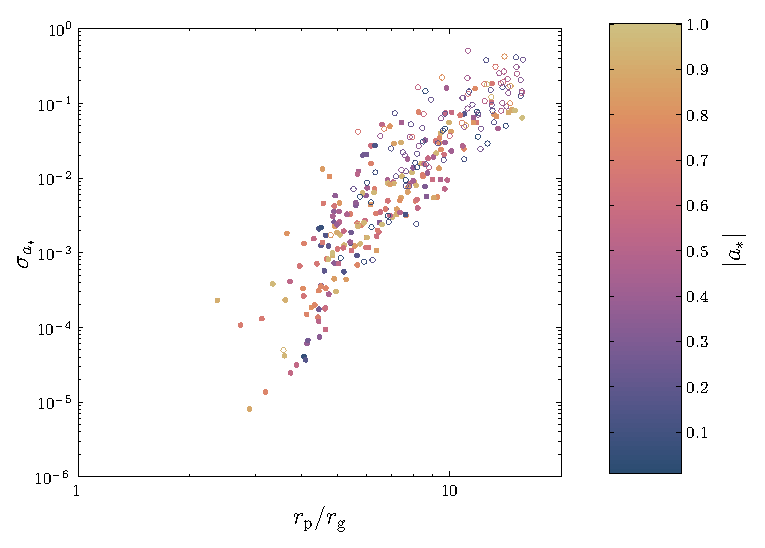
\includegraphics[width=0.48\textwidth]{./images/Fig_MCMC_sigmas_rp_spin_2}} \quad
\subfigure[Orientation angle $\Theta\sub{K}$.]{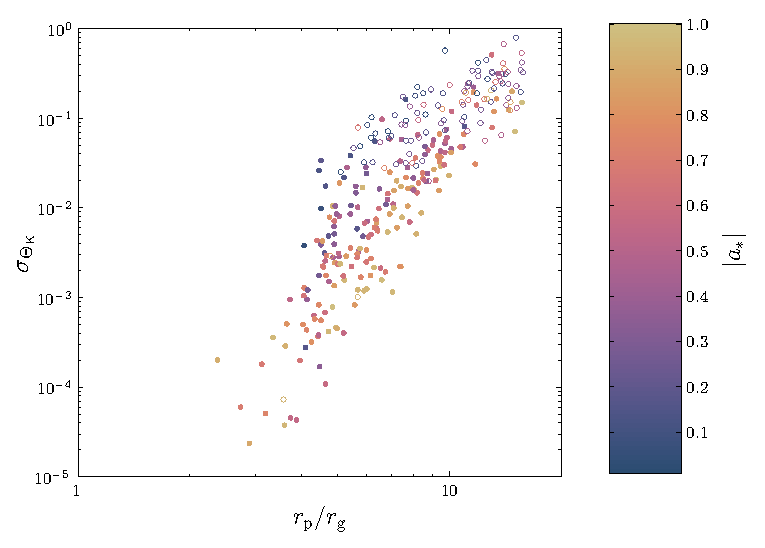
\includegraphics[width=0.48\textwidth]{./images/Fig_MCMC_sigmas_rp_spin_8}} \\
\subfigure[Orientation angle $\Phi\sub{K}$.]{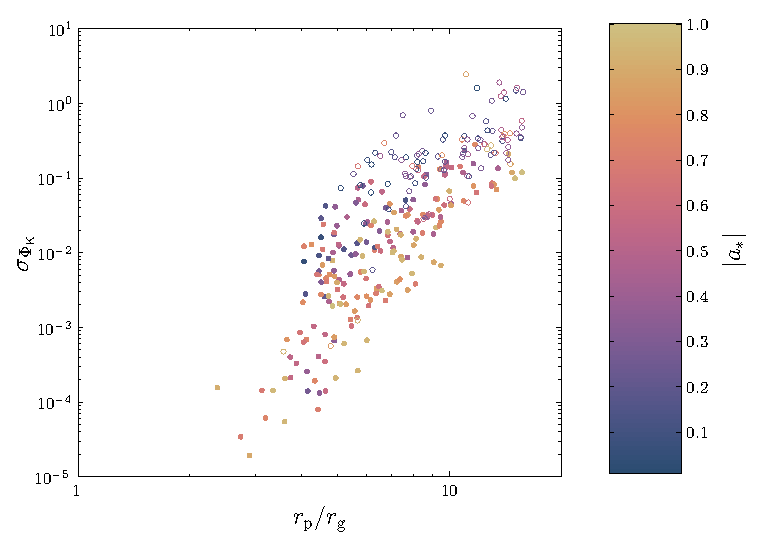
\includegraphics[width=0.48\textwidth]{./images/Fig_MCMC_sigmas_rp_spin_9}} \quad
\subfigure[Orbital inclination $\iota$.]{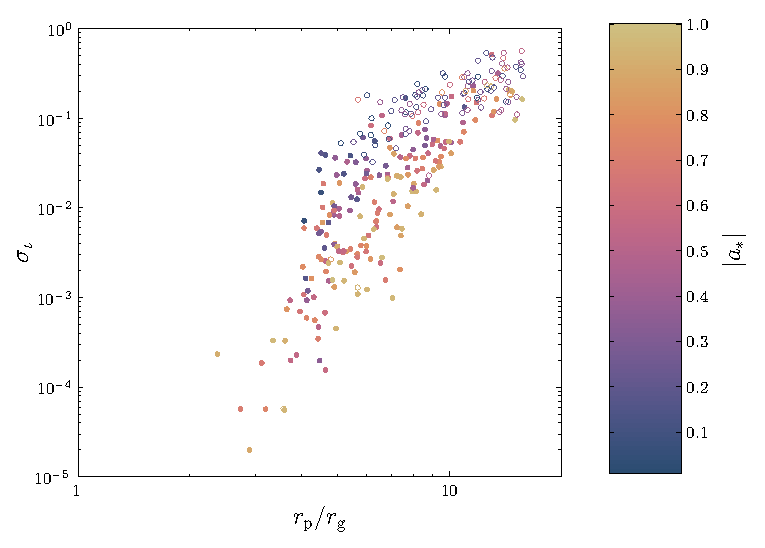
\includegraphics[width=0.48\textwidth]{./images/Fig_MCMC_sigmas_rp_spin_4}} \\
\subfigure[Periapse azimuthal phase $\phi\sub{p}$]{\includegraphics[width=0.48\textwidth]{./images/Fig_MCMC_sigmas_rp_spin_7}} \quad
\subfigure[Periapse polar phase $\chi\sub{p}$.]{\includegraphics[width=0.48\textwidth]{./images/Fig_MCMC_sigmas_rp_spin_5}}
\caption{Parameter standard deviations versus periapsis $r\sub{p}$, showing dependence (or lack thereof) upon the spin magnitude $|a_\ast|$.}
\label{fig:sigmas-spin}
\end{figure}
These parameters are defined with reference to the coordinate system established by the spin axis: for $a_\ast = 0$ we have spherical symmetry and there would be ambiguity in defining them. Therefore, it makes sense that they can be more accurately determined for larger spin magnitudes. The width for $a_\ast$, however, shows no clear correlation.

Comparing our MCMC and FIM results, we see there can be significant differences. Most parameters give results consistent to within an order (or two) of magnitude. The best agreement is for $t\sub{p}$, which is largely uncorrelated with the other parameters. The widths for $M_\bullet$, $a_\ast$, $L_\infty$ and $\iota$ show more severe differences; these parameters show the tightest degeneracies. The two methods do show signs of slowly converging with increasing SNR, as expected.

As a consistency check, to verify that the mismatch between the FIM and MCMC results is a consequence of parameter correlations, we calculated one-dimensional FIMs, only varying the MBH mass, and compared these to widths computed from MCMCs only sampling in mass. These were found to be in good agreement. The majority ($\sim 87\%$) have standard deviations consistent to within a factor of two; the rest within an order of magnitude.\footnote{One differed by more than an order of magnitude, and also failed to fulfil the (one dimensional) MM criterion; this was a numerical problem in calculating the FIM.} Some small difference is expected because of numerical error from calculating derivatives for the FIM by finite differencing.

\subsection{Scientific potential}

Having quantified the precision with which we could infer parameters from an EMRB waveform, we can now consider if it is possible to learn anything new.

Of paramount interest are the MBH mass and spin. The current uncertainty in the mass is $\sigma_{M_\bullet} = 0.36 \times 10^6 M_\odot$ ($\sim 8\%$; \citealt{Gillessen2009}). There are few runs amongst our data set that are not better than this: it appears that orbits of a $\mu = 10 M_\odot$ CO with periapses $r\sub{p} \lesssim 13 r\sub{g}$ should be able to match our current observational constraints. However, the EMRB is an independent measurement, and so a measurement of comparable precision to the current bound can still be informative. Accuracy of $1\%$ could be possible if $r\sub{p} \lesssim 8 r\sub{g}$.

The spin is less well constrained. To obtain an uncertainty for the magnitude of $0.1$, comparable to that achieved in X-ray measurements of active galactic nuclei, it appears that the periapsis needs to be $r\sub{p} \lesssim 11 r\sub{g}$. For smaller periapses, the uncertainty can be much less, indicating that an EMRB could be an excellent probe. The orientation angles for the spin axis may be constrained to better than $0.1$ for $r\sub{p} \lesssim 11 r\sub{g}$. It may well be possible to learn both the direction and the magnitude of the spin. This could illuminate the MBH's formation.

We have no {\it a priori} knowledge about the CO or its orbit, so anything we learn would be new. However, this is not particularly useful information, unless we observe multiple bursts, and can start to build up statistics for the dynamics of the GC. Using current observations for the distance to the GC, which could be further improved by the mass measurement from the EMRB, it is possible to infer a value for the mass $\mu$ from $\zeta$. This could inform us of the nature of the object (BH, NS or WD) and be a useful consistency check. A small value of $\zeta$, indicating a massive CO, is unambiguous evidence for the existence of a stellar-mass BH.

\section{Summary and conclusions}

We have analysed the properties of EMRBs from the Galactic Centre. We used NK waveforms built using spherical polar and oblate spheroidal coordinates. The two coordinate schemes yield almost indistinguishable results. There may be differences when the spin is large and the periapse is small: $\sim 10\%$ for $r\sub{p} \simeq 4 r\sub{g}$, $\sim 20\%$ for $r\sub{p} \simeq 2 r\sub{g}$. This is less than the error inherent in the semirelativistic approximation inferred from the difference in NK and BH perturbation theory energy fluxes in \secref{Energy}. We conclude that either is a valid choice for this purpose and have adopted spherical polar coordinates.

The SNR of bursts is well correlated with the periapsis, it can be reasonably described as having a power-law dependence. Using LISA, signals should be detectable for a $1 M_\odot$ ($10 M_\odot$) object if the periapse is $r\sub{p} < 27 r\sub{g}$ ($r\sub{p} < 65 r\sub{g}$), corresponding to a physical scale of $1.7 \times 10^{11}\units{m}$ ($4.1 \times 10^{11}\units{m}$) or $5.6 \times 10^{-6}\units{pc}$ ($1.3 \times 10^{-5}\units{pc}$). Using eLISA, these distances are approximately three times smaller.

We conducted an investigation using Fisher matrix analysis into how precisely we could infer parameters of the GC's MBH. However, we found that the linearised-signal approximation does not hold for these bursts over a wide range of SNR. This demonstrates the necessity of checking the approximation before quoting the results of an analysis \citep{Vallisneri2008}.

We used MCMC results as a more robust measure of parameter estimation accuracy. Potentially, it is possible to determine very precisely the key parameters defining the MBH's mass and spin, if the orbit gets close enough to the MBH. It appears that we can achieve good results from a single EMRB with periapsis of $r\sub{p} \simeq 10 r\sub{g}$ for a $10 M_\odot$ CO. This translates to a distance of $6 \times 10^{10}\units{m}$ or $2 \times 10^{-6}\units{pc}$. Orbits closer than this would place stricter constraints. The best orbits yield uncertainties of almost one part in $10^5$ for the MBH mass and spin, far exceeding existing techniques. Conversely, orbits with $r\sub{p} \gtrsim 16 r\sub{g}$ are unlikely to provide any useful information.

Before we can quote results for how accurately we can determine the various parameters, we must consider the probability of each orbit. This shall be done in \chapref{events}.

We have so far only considered EMRBS from our Galaxy; a natural extension is to consider bursts from extragalactic sources, which we do in the next chapter. Extragalactic bursts are not as promising as those from the GC, but could still make a significant contribute to the total burst event rate. 


\chapter{Extragalactic bursts}\label{ch:extragal}

It is well established that space is big \citep[chapter 8]{Adams1979}. The Milky Way, our own island universe, is but one of a multitude of galaxies. Each one of these may have an MBH nestled at its core \citep{Lynden-Bell1971, Soltan1982}. We have considered measuring the properties of the Galaxy's MBH using EMRBs and found that bursts can be informative if the periapsis is small enough. In this chapter, we extend this work to other nearby galaxies. If extragalactic EMRBs are detectable, they may be useful for constraining the properties of those galaxies' MBHs.

We use the NK waveforms from \chapref{waveforms} and the data analysis techniques from \chapref{param}. In \secref{extragal-SNR} we discuss the detectability of EMRBs from extragalactic sources. We show that bursts from other galaxies could be detected with LISA or eLISA. Following this, in \secref{extragal-Res}, we present examples of the constraints we could place using EMRBs. We conclude in \secref{extragal-End} with a discussion of our findings.

\section{Detectability of extragalactic bursts}\label{sec:extragal-SNR}

Whether or not a burst is detectable is determined by its SNR. This is calculated using \eqnref{SNR}. We assume a detection threshold of $\rho = 10$ as in \secref{Gal-SNR}. The SNR of an EMRB depends upon many parameters; for a given MBH, the most important is the periapse radius $r\sub{p}$. There is a good correlation between $\rho$ and $r\sub{p}$. Other parameters, specifying the inclination of the orbit, the orientation of the system with respect to the detector, or the MBH spin, only produce scatter about this trend. The form of the $\rho$--$r\sub{p}$ relation depends upon the noise curve.

We parameterize the detectability in terms of a characteristic frequency $f_\ast$. The speed at periapse scales like $v \sim \sqrt{GM_\bullet/r\sub{p}}$; the characteristic time taken for the position to change is then $T \sim r\sub{p}/v$, and so we define the characteristic frequency as
\begin{equation}
f_\ast = \sqrt{\dfrac{GM_\bullet}{r\sub{p}^3}}.
\end{equation}
This allows comparison between different systems where the same periapse does not correspond to the same frequency and, thus, the same point of the noise curve.

We also expect the SNR to scale with other quantities. We define a characteristic strain amplitude for a burst $h_0$; we expect $\rho \propto h_0$, where the proportionality is set by a frequency-dependent function that includes the effect of the noise curve. Assuming that the strain is dominated by the quadrupole contribution (\citealt[section 36.10]{Misner1973}; \citealt[section 17.9]{Hobson2006}) we expect
\begin{equation}
h_0 \sim \dfrac{G}{c^6}\dfrac{\mu}{R}\dfrac{\dd^2}{\dd t^2}\left(r^2\right),
\end{equation}
where $\mu$ is the CO mass, $R$ is the distance to the MBH, $t$ is time and $r$ is a proxy for the position of the orbiting object. The characteristic rate of change is set by $f_\ast$ and the characteristic length-scale is set by $r\sub{p}$. Hence
\begin{align}
h_0 \sim {} & \dfrac{G}{c^6}\dfrac{\mu}{R}f_\ast^2 r\sub{p}^2 \\
 \sim {} & \dfrac{G^{5/2}}{c^6}\dfrac{\mu}{R}f_\ast^{-2/3}M_\bullet^{2/3}.
\end{align}
Using this, we can factor out the most important dependences to give a scaled SNR defined by
\begin{equation}
\rho_\ast = \left(\dfrac{\mu}{M_\odot}\right)^{-1}\left(\dfrac{R}{\mathrm{Mpc}}\right)\left(\dfrac{M_\bullet}{10^6 M_\odot}\right)^{-2/3}\rho.
\label{eq:SNR-scaling}
\end{equation}

Space-borne detectors are most sensitive to EMR signals originating from systems containing MBHs with masses $\sim10^6 M_\odot$. Higher mass objects produce signals at too low frequencies. We considered several nearby MBHs that were likely candidates for detectable burst signals. Details are given in \tabref{MBHs}.
\begin{table}\footnotesize
%\begin{minipage}{\columnwidth}
 \centering
  \begin{tabular}{P{0.22\textwidth} c  D{.}{.}{2.5} P{0.4\textwidth}}
  \toprule
   Galaxy & \multicolumn{1}{c}{$M_\bullet/10^6 M_\odot$} & \multicolumn{1}{c}{$R/\mathrm{Mpc}$} & References \\
 \midrule
 Milky Way (Sgr A*) & $4.31 \pm 0.36$ & 0.00833 & \citet{Gillessen2009} \\
 Andromeda (M31, NGC 224) & $140^{+90}_{-30}$ & 0.770 & \citet{Bender2005,Karachentsev2004} \\
 M32 (NGC 221) & $2.5 \pm 0.5$ & 0.770 & \citet{Verolme2002,Karachentsev2004} \\
 Circinus & $1.1 \pm 0.2$ & 2.82 & \citet{Graham2008,Greenhill2003,Karachentsev2007} \\
 NGC 4945 & $1.4^{+0.7}_{-0.5}$ & 3.82 & \citet{Greenhill1997,Ferrarese2005,Karachentsev2007} \\
 Sculptor (NGC 253) & $10^{+10}_{-5}$ & 3.5 & \citet{Graham2011,Rodriguez-Rico2006,Rekola2005} \\
 NGC 4395 & $0.36 \pm 0.11$ & 4.0 & \citet{Peterson2005,Thim2004} \\
 M96 (NGC 3368) & $7.3 \pm 1.5$ & 10.1 & \citet{Graham2011,Nowak2010,Tonry2001} \\
 NGC 3489 & $5.8 \pm 0.8$ & 11.7 & \citet{Graham2011,Nowak2010,Tonry2001} \\
\bottomrule
\end{tabular}
\caption{Sample of nearby MBHs that are candidates for producing detectable EMRBs.\label{tab:MBHs}}
%\end{minipage}
\end{table}
For each, we calculated SNRs at $\sim 10^4$ different periapse distances, uniformly distributed in logarithmic space between the innermost orbit and $100 r\sub{g}$ following the procedure in \secref{wave-ex}: for each periapse, five SNRs were calculated using different sets of ancillary parameters specifying the spin magnitude and orientation of the MBH, the orbital inclination and phase, and the position of the detector.

The scaled SNRs are plotted in \figref{scaled-SNR}. 
\begin{figure}
\centering
 \includegraphics[width=0.6\textwidth]{./images/Fig_SNR_scaled_fit}
 \caption{Scaled SNR for EMRBs as a function of characteristic frequency. The fitted curve from \eqnref{scaled-SNR} is indicated by the line.}
 \label{fig:scaled-SNR}
\end{figure}
The plotted points are the average values of $\ln \rho_\ast$ calculated for each periapse distance. The curve shows that EMRB SNR does scale as expected, and $\rho_\ast$ can be described as a one-parameter curve. There remains some scatter about this: the larger scatter at low frequencies is a consequence of numerical noise from dealing with very low SNRs from Andromeda; removing the averaging over ancillary parameters increases the scatter to be typically about an order of magnitude in total. However, the fit is good enough for rough calculations.

We approximate the trend with a parameterized curve
\begin{equation}
\rho_\ast = \alpha_1 \left(\dfrac{f_\ast}{\mathrm{Hz}}\right)^{\beta_1} \left[1 + \left(\alpha_2 \dfrac{f_\ast}{\mathrm{Hz}}\right)^{\beta_2}\right]\left[1 + \left(\alpha_3 \dfrac{f_\ast}{\mathrm{Hz}}\right)^{\beta_3}\right]^{-\beta_4}.
\label{eq:scaled-SNR}
\end{equation}
To fit this, we treat the problem as if it were a likelihood maximisation, with each averaged point having a Gaussian likelihood with standard deviation defined from the scatter because of the variation in the ancillary parameters. The optimised values for LISA are
\begin{equation}
\begin{array}{c}
\alpha_1 \simeq 8.93 \times 10^4, \quad \alpha_2 \simeq 4.68 \times 10^2, \quad \alpha_3 \simeq 1.84 \times 10^2,\\
\beta_1 \simeq 1.84, \quad \beta_2 \simeq 3.23, \quad \beta_3 \simeq 1.27, \quad \beta_4 \simeq 4.13.
\end{array}
\end{equation}

Using our fitted trends, it is possible to invert \eqnref{SNR-scaling} to find the furthest distance that a system containing an MBH of a given mass can produce detectable bursts. In calculating the maximum SNR it is necessary to decide upon a maximum $f_\ast$. This corresponds to the minimum periapse radius, which is in turn determined by the MBH spin. For the optimal case with a maximally rotating MBH, the innermost periapsis is $r\sub{p} = r\sub{g}$; for a non-rotating MBH, the innermost periapsis would be $r\sub{p} = 4r\sub{g}$. We shall use both as limits for the maximum SNR.

\Figref{detect} shows the detectability limit for $\mu = 1 M_\odot$ and $\mu = 10 M_\odot$ COs. In addition to the sample of MBHs from \tabref{MBHs} we plot additional nearby MBHs \citep[see][and references therein]{Graham2008,Graham2011,Graham2013}. 
\begin{figure}
\centering
 \includegraphics[width=0.6\textwidth]{./images/Fig_M_R_detect_1}
 \caption{Limit of detection using LISA for EMRBs originating from MBHs of mass $M$ and distance $R$ with CO of mass $\mu = 1 M_\odot$ (dashed line) or $\mu = 10 M_\odot$ (solid line). The detection threshold is assumed to be $\rho = 10$. The thicker line is the limit for non-rotating MBHs, the thinner is for maximally rotating MBHs. Sources below the relevant line are potentially detectable. The crosses indicate the selected sample of MBHs used to calibrate the curve and the dots indicate other nearby MBHs with known masses. The trends should not be extrapolated to lower MBH masses.}
 \label{fig:detect}
\end{figure}
Systems containing more massive COs are detectable to a greater distance, but are also the more likely sources since mass segregation ensures that they are more likely to be on orbits that pass close to the MBH \citep{Bahcall1977, Alexander2009, Preto2010}. Limits using periapsis of $r\sub{g}$ and $4r\sub{g}$ are shown: intermediate spin values would have limits between these two. In any case, these are strict bounds; it is unlikely that we would observe a burst from the optimal orbit. Therefore bursts from MBHs outside the curve are impossible to detect and those inside may be possible, but need not be probable, to detect.

It appears that there are many extragalactic MBHs which could produce observable bursts. From the sample in \tabref{MBHs}, all could be detected. Andromeda could only be detected if it has a high spin value. It is therefore less promising than the others. NGC 3489, M96 and Sculptor lie on the boundary of detectability for non-spinning sources with a $10 M_\odot$ CO. They are therefore of marginal interest: we do not necessarily need any special requirement for the spin, but such close orbits would be infrequent. NGC 4395, NGC 4945 and Circinus are around the boundary of detectability for a $1 M_\odot$ CO. Hence, we could potentially see bursts from WDs or NSs as well as BHs. M32 is the best extragalactic source, lying safely within the detection limit for $1 M_\odot$ COs. Outside of our sample there are other MBHs with measured masses that are of interest. A great many could potentially be detected using optimal bursts from $10 M_\odot$ COs orbiting a maximally rotating MBH.\footnote{Many galaxies of the Virgo cluster fall in this category. This could potentially make identifying the source galaxy more difficult as the candidates are close together. Since we would have to be fortunate to encounter this problem, we will not be overly concerned by it.} The most promising MBHs not included in our test sample are found in M64 (NGC 4826), NGC 3076 and M94 (NGC 4736).

We can repeat the analysis for eLISA. The scaled SNRs are shown in \figref{scaled-SNR-eLISA}. 
\begin{figure}
\centering
 \includegraphics[width=0.6\textwidth]{./images/Fig_SNR_scaled_fit_eLISA}
 \caption{Scaled SNR for EMRBs as a function of characteristic frequency for the eLISA design. The fitted curve from \eqnref{scaled-SNR} is indicated by the line.}
\label{fig:scaled-SNR-eLISA}
\end{figure}
Since Andromeda was only marginally of interest for the classic LISA design, we did not include it this time. This reduces the scatter at low characteristic frequencies.

The curve is fitted with
\begin{equation}
\begin{array}{c}
\alpha_1 \simeq 73.9, \quad \alpha_2 \simeq 4.99 \times 10^3, \quad \alpha_3 \simeq 52.7,\\
\beta_1 \simeq 1.47, \quad \beta_2 \simeq 0.85, \quad \beta_3 \simeq 1.76, \quad \beta_4 \simeq 1.25.
\end{array}
\end{equation}
The fit parameters are markedly different from those for LISA. However, since we are fitting a phenomenological model and the parameters have no physical significance, we are not concerned by this. The parameters yield a good fit to the data, which is all that we require here.

Using this fit to find the detectability range results in the curves shown in \figref{detect-eLISA}. 
\begin{figure}
\centering
 \includegraphics[width=0.6\textwidth]{./images/Fig_M_R_detect_2}
 \caption{Limit of detection using eLISA for EMRBs originating from MBHs of mass $M$ and distance $R$ with CO of mass $\mu = 1 M_\odot$ (dashed line) or $\mu = 10 M_\odot$ (solid line). The detection threshold is assumed to be $\rho = 10$. The thicker line is the limit for non-rotating MBHs, the thinner is for maximally rotating MBHs. Sources below the relevant line are potentially detectable. The crosses indicate the selected sample of MBHs used to calibrate the curve and the dots indicate other nearby MBHs with known masses. The trends should not be extrapolated to lower MBH masses.}
\label{fig:detect-eLISA}
\end{figure}
The maximum distances are reduced compared to the LISA case, indicating that detectable bursts would be much rarer. There still remain a number of potential candidate galaxies. From our sample, Andromeda is on the very edge of possibility. NGC 3489, M96 and Sculptor require a high spin, making them unlikely sources. NGC 4395, NGC 4945 and Circinus can be detected without the high spin, assuming a $10 M_\odot$ CO. Of the extragalactic sources, only M32 remains detectable with a $1 M_\odot$ CO, and still it requires a non-zero spin.

Using either noise curve, we see that EMRBs could potentially be seen from a range of galaxies. The Galaxy's MBH remains securely detectable in either case. M32 is the next best. MBHs with masses $\sim 10^6$--$10^7 M_\odot$ are observable to the greatest distance. We currently know of few MBHs with masses at the lower end of the spectrum ($10^5$--$10^6 M_\odot$), but these would be good potential candidates.

\section{Parameter estimation using extragalactic bursts}\label{sec:extragal-Res}

We are not only interested in discovering if EMRBs are detectable, but also if we can extract information from the signals about their sources. To investigate the potential of extragalactic EMRBs, we considered a sample of bursts from M32, the most promising candidate; NGC N4945, which is near to the optimal mass for LISA (without assuming spin), and NGC 4395, the lightest MBH in our sample. Circinus is similar to NGC 4945, so we expect comparable results: EMRBs from Circinus should be slightly more useful as Circinus is closer.

\subsection{Parameter inference}

In determining parameters from burst waveforms, we have the same inference problem as in \secref{Estimation}. Our parameter set, as previously enumerated in \secref{Mod-param}, consists of:
\begin{enumerate}[leftmargin=*, widest=\:88--88.]
\item[1.] The MBH's mass $M_\bullet$.
\item[2.] The spin parameter $a_\ast$.
\item[3, 4.] The orientation angles for the MBH spin $\Theta\sub{K}$ and $\Phi\sub{K}$.
\item[5.] The source distance $R$ divided by the CO mass $\mu$, which we denote as $\zeta = R/\mu$. This scales the amplitude of the waveform.
\item[6, 7.] The angular momentum of the CO parameterized in terms of total angular momentum $L_\infty$ and inclination $\iota$.
\item[8--10.] The angular phases at periapse, $\phi\sub{p}$  and $\chi\sub{p}$ (which determines $\theta\sub{p}$), and the time of periapse $t\sub{p}$.
\item[11, 12.] The coordinates of the source. Sky position is already determined to high accuracy for each galaxy. Since an EMRB can only give weak constraints on source position we take it as known and do not infer it.
\item[13, 14.] The orbital position of the detector. This should be known and need not be inferred. We assume the same initial position as \citet{Cutler1998}; this does not qualitatively influence results.
\end{enumerate}
We are interested in inferring the first $10$. The most interesting are the MBH's mass and spin, as these give an insight into the evolution of the MBH's host galaxy. We have estimates for many extragalactic MBHs' masses, but these are less accurate than for the Galactic MBH.

We have assumed that sky position is known; to be able to do this in practice we must be able to successfully identify the source galaxy. We shall see that there are only a few potential galaxies that could produce detectable EMRBs. It should, therefore, not be too computationally expensive to check all the candidate sky positions. If multiple galaxies lie close together on the sky, such that they cannot be distinguished, it could be possible to use constraints on the MBH mass to differentiate them. This would not help with galaxies for which we do not have good MBH mass estimates.

\subsection{Mapping the posterior distribution}

To discover if any parameters can be accurately inferred, we must characterise the shape of the posterior. We do this using the MCMC techniques developed in \secref{MCMC}. The only modification was to lower the target acceptance rate to $\sim0.08$. This appeared to give improved convergence for these less informative distributions.

As for bursts from the GC, posteriors can show strong and complicated parameter degeneracies. The lower SNR compared to Galactic bursts yields wider distributions. As the periapsis increases, the posteriors deteriorate, becoming uninformative. The posteriors recovered from our MCMC show a wide variety of forms. There is a spectrum from well-formed Gaussians through elongated ellipsoids to complete covering of the parameter range. Some example results are shown in \figref{MCMC-a}, \ref{fig:MCMC-b} and \ref{fig:MCMC-c}. These are similar to the plots in \secref{Gal-Results} except that we now plot $\ln(M_\bullet/M_\odot)$ and $\ln(\zeta/\zeta_0)$.

\begin{figure}%[ht]
\centering
\vspace{0.5\baselineskip}
   \includegraphics[width=0.8\textwidth]{./images/Fig_M32_MCMC_193_triangle_40}
\caption{Marginalised one- and two-dimensional posteriors (on the diagonal and above, respectively). The scales are identical in both types of plots. The dotted line indicates the true value. These distributions are exceptionally cromulent and well converged. Angular momentum is in units of $L_\bullet = GM c^{-1}$ and the scaled distance is in units of $\zeta_0 = 1 M_\odot^{-1}\units{kpc}$. The EMRB is from M32 and has $r\sub{p} \simeq 5.53 r\sub{g}$.}
\label{fig:MCMC-a}
\end{figure}
\Figref{MCMC-a} shows the posterior for an EMRB from M32 with $r\sub{p} \simeq 5.53 r\sub{g}$. The distribution is well-defined and near Gaussian, although even in this best case the presence of degeneracies is clear. This example illustrates that it is possible to obtain good results, similar to those from the GC, from extragalactic sources. Unfortunately, such tight distributions are not common in our sample.

\begin{figure}%[ht]
\centering
\vspace{0.5\baselineskip}
   \includegraphics[width=0.8\textwidth]{./images/Fig_N4395_MCMC_120_triangle_40}
\caption{Marginalised one- and two-dimensional posteriors. The conventions are the same as in \figref{MCMC-a}. These distributions begin to show the complicated shapes of degenerate distributions. The EMRB is from NGC 4395 and has $r\sub{p} \simeq 5.92 r\sub{g}$.}
\label{fig:MCMC-b}
\end{figure}
\Figref{MCMC-b} shows the posterior for an EMRB from N4395 with $r\sub{p} \simeq 5.92 r\sub{g}$; it illustrates a more usual posterior. Typical posteriors are not Gaussian; the forms vary significantly, such that it is not possible to produce a standard shape. Non-Gaussianity manifests by the distributions broadening, developing curves and becoming banana-like. The degeneracies may evolve such that there are multiple modes.

\begin{figure}%[ht]
\centering
	\vspace{0.5\baselineskip}
   \includegraphics[width=0.8\textwidth]{./images/Fig_M32_MCMC_159_triangle_40}
\caption{Marginalised one- and two-dimensional posteriors. The conventions are the same as in \figref{MCMC-a}. These are the worst-case scenario distributions that are uninformative. The EMRB is from M32 and has $r\sub{p} \simeq 11.79 r\sub{g}$.}
\label{fig:MCMC-c}
\end{figure}
\Figref{MCMC-c} shows the culmination of the deterioration of the posterior; it is for an EMRB from M32 with $r\sub{p} \simeq 11.79 r\sub{g}$. In this case, the distributions have extended to encompass the entire range for some parameters and so the EMRB is (near) useless. The posteriors show intricate degeneracies in some angular parameters. These are naturally periodic and demonstrate that near identical bursts can be produced through various rotations of the MBH and orbit. Such bursts are not informative and so are not of interest, but we include this example so that there is no illusion of all EMRBs having perfect posteriors.

The general trend is for bursts from orbits with smaller periapses to be narrower and more Gaussian. As the periapse increases, and SNR decreases, the distributions broaden becoming more non-Gaussian. Curving degeneracies and secondary modes develop. Eventually, the distribution broadens to encompass the entire permitted range for the spin and various angular parameters, effectively making these quantities unconstrained.

\subsection{Parameter uncertainties}

Characteristic distribution widths for the (logarithm of the) MBH mass and the spin are shown in \figref{sigmas-M32}, \ref{fig:sigmas-N4945} and \ref{fig:sigmas-N4395} for M32, NGC 4945 and NGC 4395 respectively. Plotted are the standard deviation $\sigma\sub{SD}$ and the half-width of the $p = 0.68$ range calculated from the $k$-d tree $\sigma_{0.68}$. These widths are defined in \secref{k-d} and are equal for a Gaussian distribution. The filled circles are used for runs that appear to have converged. The open circles are for those yet to converge, but which appear to be approaching an equilibrium state; widths should be accurate to within $\sim 10\%$.
\begin{figure}%[htp]
\centering
\subfigure[Natural logarithm of MBH mass.]{\includegraphics[width=0.475\textwidth]{./images/Fig_M32_MCMC_sigmas_rp_1}} \quad
\subfigure[Dimensionless spin.]{\includegraphics[width=0.475\textwidth]{./images/Fig_M32_MCMC_sigmas_rp_2}} \\
\caption{Distribution widths as functions of periapsis $r\sub{p}$ for M32. The light blue points are used for the standard deviation, the black for the $68$-percentile half-width. The filled circles are converged runs and the open circles for those yet to converge. The dotted line is the current uncertainty for $M_\bullet$. The dashed line is the standard deviation for a uniform $a_\ast$ distribution and the dot--dashed line is the equivalent $68$-percentile half-width.}
\label{fig:sigmas-M32}
\end{figure}
\begin{figure}%[htp]
\centering
\subfigure[Natural logarithm of MBH mass.]{\includegraphics[width=0.475\textwidth]{./images/Fig_N4945_MCMC_sigmas_rp_1}} \quad
\subfigure[Dimensionless spin.]{\includegraphics[width=0.475\textwidth]{./images/Fig_N4945_MCMC_sigmas_rp_2}} \\
\caption{Distribution widths as functions of periapsis $r\sub{p}$ for NGC 4945. Conventions are identical to those in \figref{sigmas-M32}.}
\label{fig:sigmas-N4945}
\end{figure}
\begin{figure}%[htp]
\centering
\subfigure[Natural logarithm of MBH mass.]{\includegraphics[width=0.475\textwidth]{./images/Fig_N4395_MCMC_sigmas_rp_1}} \quad
\subfigure[Dimensionless spin.]{\includegraphics[width=0.475\textwidth]{./images/Fig_N4395_MCMC_sigmas_rp_2}} \\
\caption{Distribution widths as functions of periapsis $r\sub{p}$ for NGC 4395. Conventions are identical to those in \figref{sigmas-M32}.}
\label{fig:sigmas-N4395}
\end{figure}

The widths, corresponding to potential parameter accuracies, improve rapidly with decreasing periapsis. The two widths, $\sigma\sub{SD}$ and $\sigma_{0.68}$, are typically of similar sizes, despite manifest non-Gaussianity. This is true for all parameters: the greatest differences are when the distributions are strongly multimodal. The fractional difference between the two widths may be up to $\sim 40\%$ for $\ln(M/M_\odot)$ and $a_\ast$; the widths for $\phi\sub{p}$ show the greatest difference, where $\sigma\sub{SD}$ may be a factor of a few larger than $\sigma_{0.68}$. Both $\sigma\sub{SD}$ and $\sigma_{0.68}$ tend to the appropriate limits for uninformative distributions.

In the best case, uncertainties in mass and spin may be only one part in $10^2$. As might be expected from \figref{detect}, M32 has the smallest widths, followed by NGC 4945 and then NGC 4395. The spin width saturates about the value expected from a uniform distribution. At this point, we can no longer constrain the spin. The transition does not show any clear correlation with the magnitude of the spin, but is predominantly determined by the periapsis and SNR.

The other parameters show similar behaviour. The angular variables also reach maximum widths, corresponding to uninformative distributions. This does not appear to be directly tied to the spin width.

Potentially, an EMRB could place useful constraints on the mass and spin of an MBH if the periapse radius is small enough.\footnote{Here, we assume that a mass measurement is useful if its accuracy is smaller than the current measurement uncertainty, and a spin measurement is useful if it provides any constraint.} For M32 we require $r\sub{p} \lesssim 8 r\sub{g}$; for NGC 4945 we require $r\sub{p} \lesssim 8 r\sub{g}$ and $r\sub{p} \lesssim 7 r\sub{g}$ for mass and spin measurements, respectively, and for NGC 4395 we require $r\sub{p} \lesssim 9 r\sub{g}$ and $r\sub{p} \lesssim 8 r\sub{g}$, respectively. Since the range of useful periapses is small, we expect useful EMRBs originating from any individual galaxy to be rare. However, because there are many galaxies hosting potential sources, the probability of seeing any useful EMRBs need not be negligible. Therefore, EMRBs could be a useful astronomical tool.

\section{Summary and conclusions}\label{sec:extragal-End}

We have studied EMRBs from extragalactic sources. The SNR of EMRBs has a fundamental scaling with the system parameters. Removing these proportionalities gives a scaled SNR that can be specified as a function of the characteristic frequency $f_\ast$. Using these relations allows us to calculate the maximum distance to which EMRBs from a system containing an MBH of a given mass can be detected.

The MBH in our own Galaxy is by far the best source for bursts; however, it is also possible to detect bursts from extragalactic sources. In particular, M32 is a promising candidate. This is good news for any space-borne GW detectors, as EMRBs can be added to their list of potential sources.

Utilising the classic LISA design, EMRBs from a $10 M_\odot$ orbiting CO could be detected out to a distance of $\sim 100\units{Mpc}$. With the descoped eLISA design, this decreases to $\sim 10\units{Mpc}$. This may drastically reduce the chance of observing an EMRB. For both detectors, sensitivity is maximal for MBHs of $M_\bullet \sim 10^6$--$10^7 M_\odot$, being at slightly higher masses for LISA than for eLISA. We can detect bursts from systems with high MBH spins out to a greater distance; hence, the EMRB event rate would be enhanced if MBH spins naturally tend to higher values, perhaps as a consequence of accretion.

However, we must still be cautious: EMRBs may be rare and the event rate may prevent us from observing any over a realistic mission lifetime. Bursts from any given extragalactic source should be less common than from the GC, although this may be slightly ameliorated by the larger number of galaxies hosting potential source systems. In \chapref{events} we shall construct a model to estimate the event rate for Galactic bursts. It is more difficult to perform a similar estimation for other galaxies as we do not have as detailed astrophysical measurements. However, we may use the Galactic event rate as a guide to predict the number of bursts, and we do so in \secref{extragal-events}.

Extragalactic EMRBs can provide good measurements of MBH mass and spin, but only across an extremely narrow range of periapses. We studied M32, NGC 4945 and NGC 4395 as examples. For all three we found that it is possible to extract information from bursts. The uncertainty may be one part in $10^2$--$10^3$ for M32, and slightly worse for NGC 4945 and NGC 4395, at about one part in $10^2$. These are not as good as the constraints from Galactic EMRBs, where the uncertainties could be as small as one part in $10^4$, but would still be of great astrophysical interest. These extragalactic MBHs are much harder to study than the MBH in our own Galaxy, and we have not yet been able to measure a spin value even for that MBH. Any measurement of spin would give us a unique glimpse into the formation history of the host galaxy.

%These results have been obtained assuming the classic LISA design. The first millihertz space-borne interferometer is likely to have a descoped design such as the proposed eLISA. This concept could be revised in the near future and so we have not used it to produce results. The effect of the reduced sensitivity would be to reduce the SNR and increase the widths of the posterior distributions. We expect the trends in \figref{sigmas-M32}, \ref{fig:sigmas-N4945} and \ref{fig:sigmas-N4395} to move upwards and saturate at smaller periapses.

EMRBs could be used to place useful constraints on the mass and spin of a nearby MBH if the periapse radius is small enough. Considering the promising candidates of M32, NGC 4945 and NGC 4395, we find that $r\sub{p} \lesssim 8 r\sub{g}$ typically gives insightful constraints. Such orbits are likely to be rare, but just a single such burst from any of the potential galaxies could give us information that is otherwise inaccessible. This is a tantalising prospect.


\chapter{Event rates and expectations for Galactic bursts}\label{ch:events}

For EMRBs to be a valuable astronomical tool we require the bursts to be loud enough to be detected; to contain sufficient information to improve our knowledge of their source systems, and to have a sufficiently high event rate that we expect to observe them over a mission lifetime. We have previously found that bursts can satisfy the first two requirements: in \chapref{param} we found Galactic bursts can be informative if the periapse distance is $r\sub{p} \lesssim 16 r\sub{g}$ and in \chapref{extragal} we found that the most promising extragalactic bursts could be informative if $r\sub{p} \lesssim 8 r\sub{g}$. We address the final requirement in this chapter.

We calculate the event rate for Galactic bursts. We only model our own Galaxy as it is the only galaxy for which we have reliable astronomical measurements of the parameters which determine the event rate. Previously, the best estimate for the event rate was given by \citet{Hopman2007}; they predicted an event rate for LISA of $\Gamma \sim 1\units{yr^{-1}}$. We follow a similar approach, but make a number of improvements, using NK waveforms to calculate the SNR and building a more detailed model for the GC's nuclear star cluster (NSC). We go on to use our event rate to define an expectation for the amount of information we could learn about the Galaxy's MBH using EMRBs.

\section{Calculating event rates}\label{sec:Rates}

Having determined how to generate a waveform and extract the information from it, we must now consider how likely it is that such a waveform would be observed. We wish to calculate the event rate for EMRBs, the probability that there is an encounter between a CO, on an orbit described by eccentricity $e$ and periapse radius $r\sub{p}$, and the MBH. To do so we must build a model to describe the distribution of COs about the MBH. The number density of stars in the six-dimensional phase space of position and velocity is described by the distribution function (DF) $f$ \citep[section 4.1]{Binney2008}. We introduce approximate forms for the DF appropriate for describing the NSC in \secref{DF}. These are calibrated using the simulations of \citet{Alexander2009}, the parameters of which, together with the others used to describe the Galactic NSC, are given in \secref{GC-Param}. Having set the distribution of COs, we explain how to convert this to an event rate in \secref{e-rp}. In \eqnref{Gamma} we give an expression that relates the event rate for an orbit $\Gamma(e,\,r\sub{p})$ and the DF. There is one final consideration before we can calculate the total event rate: that there is an inner periapsis inside of which orbits become depopulated. This is carefully explained in \secref{inner-cut}. We consider tidal disruption and collisions, which we assume truncate the DF at a finite periapsis so that the event rate inside these cut-offs is zero. We also consider GW inspiral, which we assume alters the event rate by modifying the distribution of COs away from its relaxed state. With these inner cut-offs established, we have completely defined the event rate distribution. This can then give the probability of an EMRB and the total event rates, which are presented in \secref{no-events}.

\subsection{The distribution function for the nuclear star cluster}\label{sec:DF}

Following the work of \citet{Bahcall1976, Bahcall1977}, we assume the DF within the NSC is only a function of the orbital energy \citep{Shapiro1978}. The energy per unit mass of the orbit is
\begin{equation}
E = \dfrac{v^2}{2} - \dfrac{GM_\bullet}{r},
\end{equation}
where $v$ is orbital velocity. The number of stars is
\begin{equation}
N = \int \dd^3r \int \dd^3v f(E).
\end{equation}
Close to the centre of the NSC, the dynamics are dominated by the influence of the MBH as it is significantly more massive than the surrounding stars. Its radius of influence is
\begin{equation}
r\sub{c} = \dfrac{GM_\bullet}{\sigma^2},
\label{eq:r_c}
\end{equation}
where $\sigma^2$ is the line-of-sight velocity dispersion \citep{Frank1976}. We assume that the mass of stars enclosed within $r\sub{c}$ is greater than the $M_\bullet$, which, in turn, is much greater than the mass of a typical star $M_\star$ \citep{Bahcall1976}. We define a reference number density $n_\star$ from the enclosed mass $m_\ast(r)$ such that
\begin{equation}
m_\star(r\sub{c}) = \dfrac{4\pi r\sub{c}^3}{3}n_\star M_\star.
\end{equation}
Within the NSC, the DF can be calculated using the approximation of the Fokker--Planck formalism \citep[section 7.4]{Binney2008}. The population of bound stars is evolved numerically until a steady state is reached, whilst the unbound stars form a reservoir with an assumed Maxwellian distribution. Denoting a species of star by its mass $M$, the unbound DF is
\begin{equation}
f_M(E) = \dfrac{C_M n_\star}{(2\pi\sigma_M^2)^{3/2}} \exp\left(-\dfrac{E}{\sigma_M^2}\right),\quad E > 0,
\label{eq:Unbound_DF}
\end{equation}
where $C_M$ is a normalisation constant.\footnote{$C_M$ determines the population ratios of species $M$ far from the MBH \citep{Alexander2009}.} If different stellar species are in equipartition, as assumed by \citet{Bahcall1976, Bahcall1977}, we expect
\begin{equation}
M \sigma_M^2 = M_\star \sigma_\star^2.
\end{equation}
However, if the unbound stellar population has reached equilibrium by violent relaxation, all mass groups are expected to have similar dispersions:
\begin{equation}
\sigma_M = \sigma_\star = \sigma,
\end{equation}
and we have equipartition of energy per unit mass \citep{Lynden-Bell1967}. This is assumed here following \citet{Alexander2009} and \citet{O'Leary2009}. The steady-state DF is largely insensitive to this choice \citep{Bahcall1977, Alexander2009}.

For bound orbits, the DF can be approximated as a power law \citep{Peebles1972}
\begin{equation}
f_M(E) = \dfrac{k_M n_\star}{(2\pi\sigma^2)^{3/2}}\left(-\dfrac{E}{\sigma^2}\right)^{p_M},\quad E < 0.
\label{eq:Bound_DF}
\end{equation}
The exponent $p_M$ varies depending upon the mass of the object, determining mass segregation. For a system with a single mass component $p = 1/4$ \citep{Bahcall1976, Young1977}. The normalisation constant $k_M$ reflects the relative abundances of the different species.\footnote{For a single mass population ($p = 1/4$) $k = 2 C$ gives a fit correct to within a factor of two \citep{Bahcall1976,Keshet2009}, we assume this holds for the dominant species of stars as, although it changes slightly with $p$, variation is small compared to errors introduced by fitting a simple power law \citep{Hopman2006, Alexander2009}.}

These cusp profiles should exist if the system has had sufficient time to become gravitationally relaxed. There is current debate about whether this may be the case, both for the GC and galaxies in general. This is discussed further in \secref{tauGC}. For concreteness, we assume a cusp has formed. If a cusp has not formed, we expect there to be a shallower core profile, with fewer objects passing close to the MBH. Our results are therefore an upper bound on possible event rates \citep{Merritt2010a,Antonini2011,Gualandris2012}. 

\subsection{Model parameters}\label{sec:GC-Param}

To describe the GC, we assume $M_\bullet = (4.31 \pm 0.36) \times 10^6 M_\odot$ \citep{Gillessen2009} and $\sigma = (103 \pm 20)\units{km\,s^{-1}}$ \citep{Tremaine2002}. This gives an NSC radius of $r\sub{c} = (1.7 \pm 0.7)\units{pc}$. Using the results of \citet{Ghez2008} we would expect the total mass of stars in the NSC to be $m_\star(r\sub{c}) = 6.4 \times 10^6 M_\odot$, which is within $5\%$ of the value obtained similarly from \citet{Genzel2003}. This gives a reference stellar density of $n_\star = 2.8 \times 10^5\units{pc^{-3}}$.

For the distribution of COs, we use the Fokker--Planck model of \citet{Hopman2006, Hopman2006a} and \citet{Alexander2009}. This includes four species: MS stars, WDs, NSs and stellar-mass BHs. Their properties are summarised in \tabref{HA}. 
\begin{table}\footnotesize
\centering
\begin{tabular}{l D{.}{.}{2.1} D{.}{.}{1.3} D{.}{.}{1.1} D{.}{.}{1.3}} 
\toprule
  Star & \multicolumn{1}{c}{$M/M_\odot$} & \multicolumn{1}{c}{$C_M/C_\star$} & \multicolumn{1}{c}{$p_M$} & \multicolumn{1}{c}{$k_M/k_\star$\footnote{\citet*{Toonen2009}}}  \\ \midrule
  MS & 1.0 & 1 & -0.1 & 1 \\
  WD & 0.6 & 0.1 & -0.1 & 0.09 \\
  NS & 1.4 & 0.01 & 0.0 & 0.01  \\
  BH & 10 & 0.001 & 0.5 & 0.008 \\
\hline
\end{tabular}
\caption{Stellar model parameters for the Galactic NSC using the results of \citet{Alexander2009}. The MS star is used as a reference for the normalisation constants. The number fractions for unbound COs are estimates corresponding to a model of continuous star formation \citep{Alexander2005}; \citet{O'Leary2009} arrive at the same proportions.}\label{tab:HA}
\end{table}
The behaviour of the Fokker--Planck model has been verified by $N$-body simulations \citep{Baumgardt2004,Preto2010}. The spatial densities of the species as specified by the Fokker--Planck models are shown in \figref{spatial-density}. 
\begin{figure}%[ht]
  \centering
  \vspace{0.2\baselineskip}
  \includegraphics[width=0.6\textwidth]{./images/Fig_spatial_density}
    \caption{Spatial density of COs as given by the Fokker--Planck models of \citet{Alexander2009}. The distributions include both bound and unbound COs. No inner cut-offs have been applied.}   
    \label{fig:spatial-density} 
\end{figure}
The steeper power law for BHs means they segregate about the MBH. Extrapolating, they would dominate in place of MS stars for radii $r < 10^{-4}r\sub{c}$. The distributions are truncated by various processes at small radii as described in \secref{inner-cut}.

Binaries may form in the NSC, encouraged by its high stellar density \citep{O'Leary2009}. However the binary fraction is still expected to be small \citep{Hopman2009}. Binaries are also disrupted by the MBH for periapses smaller than
\begin{equation}
r\sub{B} \simeq \left(\dfrac{M_\bullet}{M_1 + M_2}\right)^{1/3}a\sub{B},
\end{equation}
where $M_1$ and $M_2$ are the masses of the binary's components, and $a\sub{B}$ is the binary's semimajor axis, cf.\ \eqnref{Tidal} below. Thus, we ignore the possible presence of binaries.

\subsection{The event rate in terms of eccentricity and periapsis}\label{sec:e-rp}

We characterise orbits by their eccentricity $e$ and periapse radius $r\sub{p}$. The latter, unlike the semimajor axis, is always well defined regardless of eccentricity. For Keplerian orbits, the energy $E$ and angular momentum $L$ per unit mass are entirely characterised by these parameters
\begin{equation}
\label{eq:Energy_ecc}
\begin{split}
E & = -\dfrac{GM_\bullet(1 - e)}{2r\sub{p}}; \\
L^2 & = GM_\bullet(1 + e)r\sub{p}.
\end{split}
\end{equation}
The DF is defined per element of phase space: it is necessary to change variables from position and velocity to eccentricity and periapsis. We decompose the velocity into three orthogonal components: radial $v_r$, azimuthal $v_\phi$ and polar $v_\theta$. We assume the NSC is spherically symmetric \citep{Genzel2003, Schodel2007}, therefore we are interested in the combination
\begin{equation}
v_\perp^2 = v_\phi^2 + v_\theta^2 = v^2 - v_r^2.
\end{equation}
Under this change of variables
\begin{equation}
\dd^3v = \dd v_r \dd v_\phi \dd v_\theta \rightarrow 2\pi v_\perp \,\dd v_r \,\dd v_\perp.
\end{equation}
The specific energy and angular momentum are given by
\begin{equation}
\begin{split}
E & = \dfrac{v_r^2 + v_\perp^2}{2} - \dfrac{GM_\bullet}{r}; \\
L^2 & = r^2 v_\perp^2.
\end{split}
\end{equation}
Combining these with our earlier expressions in terms of $e$ and $r\sub{p}$,
\begin{align}
v_\perp^2 = {} & \dfrac{GM_\bullet(1 + e)r\sub{p}}{r^2}, \\
v_r^2 = {} & GM_\bullet\left[\dfrac{2}{r} - \dfrac{(1 - e)}{r\sub{p}} - \dfrac{(1 + e)r\sub{p}}{r^2}\right].
\end{align}
From the latter we can verify that the turning points of an orbit occur at
\begin{equation}
r = r\sub{p}, \quad \dfrac{1+e}{1-e}r\sub{p};
\end{equation}
the periapse is the only turning point for orbits with $e > 1$. Since we now have expressions for $\{v_r, v_\perp\}$ in terms of $\{e, r\sub{p}\}$, we can 
calculate the Jacobian
\begin{equation}
\left|\dfrac{\partial(v_r, v_\perp)}{\partial(e, r\sub{p})}\right| = \recip{2v_rv_\perp}\dfrac{e}{r\sub{p}}\left(\dfrac{GM_\bullet}{r}\right)^2.
\end{equation}
Using this, we may
rewrite our velocity element as
\begin{equation}
\dd^3v \rightarrow \dfrac{\pi e}{v_rr\sub{p}}\left(\dfrac{GM_\bullet}{r}\right)^2\,\dd e \,\dd r\sub{p}.
\end{equation}
As a consequence of our assumed spherical symmetry, 
the volume element is
\begin{equation}
\dd^3r \rightarrow 4\pi r^2 \,\dd r.
\end{equation}
Thus, 
the phase space volume element can be expressed as
\begin{equation}
\dd^3r\dd^3v \rightarrow \dfrac{4\pi^2(GM_\bullet)^2e}{v_rr\sub{p}}\,\dd r\,\dd e \,\dd r\sub{p}.
\end{equation}
The number of stars in an element $\dd r\,\dd e\,\dd r\sub{p}$ is
\begin{equation}
n(r, e, r\sub{p}) = \dfrac{4\pi^2(GM_\bullet)^2e}{v_rr\sub{p}}f(E).
\end{equation}

From this, we can construct the expected number of stars on orbits defined by $\{e, r\sub{p}\}$. The number of stars found in a small radius range $\delta r$ with given orbital properties is
\begin{equation}
n(r, e, r\sub{p})\delta r = N(e, r\sub{p}; r)\dfrac{\delta t}{P(e, r\sub{p})},
\end{equation}
where $N(e, r\sub{p}; r)$ is the total number of stars with orbits given by $\{e, r\sub{p}\}$ defined at $r$, $\delta t$ is the time spent in $\delta r$ and $P(e, r\sub{p})$ is the period of the orbit. We defer the definition of this time for unbound orbits for now. The time spent in the radius range is
\begin{equation}
\delta t = 2\dfrac{\delta r}{v_r},
\end{equation}
where the factor of two accounts for inwards and outwards motion. Hence
\begin{align}
N(e, r\sub{p}; r) = {} & \recip{2} v_r P(e, r\sub{p}) n(r, e, r\sub{p}) = \dfrac{2\pi^2(GM_\bullet)^2 e P(e, r\sub{p})}{r\sub{p}}f(E).
\end{align}
The right hand side is independent of position, subject to the constraint that the radius is in the allowed range for the orbit $r\sub{p} \leq r \leq (1+e)r\sub{p}/(1-e)$, and so $N(e, r\sub{p}) \equiv N(e, r\sub{p}; r)$. This is a consequence of the DF being dependent only upon a constant of the motion.\footnote{See \citet{Bahcall1976} equation (9) for a similar result.}

If a burst of radiation is emitted each time a star passes through periapse, the event rate for burst emission from orbits with parameters $\{e, r\sub{p}\}$ is given by
\begin{align}
\Gamma(e, r\sub{p}) = {} & \dfrac{N(e, r\sub{p})}{P(e, r\sub{p})} = \dfrac{2\pi^2(GM_\bullet)^2 e}{r\sub{p}}f(E).
\label{eq:Gamma}
\end{align}
The orbital period drops out from the calculation, so we do not have to worry about an appropriate definition for unbound orbits.

%From the event rate we may define a probability of seeing a given number of events subject to the assumption they are uncorrelated: it is given by the Poisson distribution. The probability of there being $r$ events is
%\begin{equation}
%\Pr(r|\Gamma(e, r\sub{p})) = \dfrac{\Gamma^r\exp(-\Gamma)}{r!}.
%\end{equation}
%The probability of there being a burst from an orbit with periapse $r\sub{p}$ and eccentricity $e$ is hence
%\begin{equation}
%\Pr(r \neq 0|\Gamma(e, r\sub{p})) = 1 - \Pr(r = 0|\Gamma(e, r\sub{p})).
%\end{equation}

%To estimate the expectation of a quantity across all orbits we use
%\begin{equation}
%\left\langle X\right\rangle = \sum\sub{R} \int_0^\infty \dd e \int_0^\infty \dd r\sub{p} X(r;r\sub{p},e)\Pr(r|\Gamma(e, r\sub{p})).
%\end{equation}
%Since the probability decays rapidly for large $r$, we may truncate the sum to give the required level of accuracy,

To generate a representative sample for the orbital parameters $e$ and $r\sub{p}$, we use $\Gamma(e, r\sub{p})\dd e\, \dd r\sub{p}$ as the rate for a Poisson distribution.

The total event rate can be found by integrating $\Gamma(e,\,r\sub{p})$, but before we can do this we must set the limits of the integral. The maximum periapse is set by the limit of detectability. It is particular to the detector. The inner periapse is set by physical processes. These are explained in the following section.

\subsection{The inner cut-off}\label{sec:inner-cut}

From \eqnref{Gamma} we see the event rate is highly sensitive to the smallest value of the periapsis. Ultimately the orbits cannot encroach closer to the MBH than its last stable orbit. This depends upon the spin of the MBH, but is of the order of its Schwarzschild radius. Before we reach this point, there are other processes that may intervene to deplete the orbiting stars. Our treatment of these is approximate, but should produce reasonable estimates. We consider three processes: tidal disruption by the MBH (\secref{Tidal}); GW inspiral (\secref{GW-in}), and collisional disruption (\secref{Collision}). Tidal disruption imposes a definite (albeit approximate) cut-off, while the others use statistical arguments. For these methods, we will need to define a reference time-scale for relaxation. This is done in \secref{Relax}, with further details found in \chapref{relax}.

The calculated inner cut-offs for the four stellar species across the range of bound orbits are shown in \figref{Cuts}.
\begin{figure}%[ht]
\centering
   \subfigure[{MS stars}]{\includegraphics[width=0.475\textwidth]{./images/Fig_Inner_cut_1.eps}} \quad 
   \subfigure[{WDs}]{\includegraphics[width=0.475\textwidth]{./images/Fig_Inner_cut_2.eps}} \\
   \subfigure[{NSs}]{\includegraphics[width=0.475\textwidth]{./images/Fig_Inner_cut_3.eps}} \quad
   \subfigure[{BHs}]{\includegraphics[width=0.475\textwidth]{./images/Fig_Inner_cut_4.eps}}
\caption{Inner cut-off radii for the GC as a function of eccentricity. The solid line is the Schwarzschild radius of the MBH; this gives an indication of the innermost possible orbit, which actually varies with MBH spin as well as orbital eccentricity and inclination. The dashed line is the tidal radius, which is a hard cut-off inside of which there should be no undisrupted stars. The dot--dashed line is the collisional cut-off, which is a statistical cut-off inside of which we do not expect any stars. The dotted line is the transition to the GW-dominated inspiral regime; inside of this we expect inspiralling stars in place of the relaxed distribution.}\label{fig:Cuts}
\end{figure}
The tidal and collisional disruption cut-offs are hard boundaries, inside of which we assume there are no bursting sources. The transition to the GW inspiral dominated regime marks the end of the relaxed distribution of stars; inside of this there are only inspiralling stars.

\subsubsection{Tidal disruption}\label{sec:Tidal}

Tidal forces from the MBH can disrupt stars. This occurs at the tidal radius
\begin{equation}
r\sub{T} \simeq \left(\dfrac{M_\bullet}{M}\right)^{1/3}R_M,
\label{eq:Tidal}
\end{equation}
where $R_M$ is the radius of the star \citep{Hills1975, Rees1988, Kobayashi2004}.\footnote{See \citet{Kesden2012} for a general relativistic treatment.} Any star on an orbit with $r\sub{p} < r\sub{T}$ is disrupted in the course of its orbit. Parameterizing orbits by their periapsis allows us to easily determine which stars should be disrupted. We do not include the full effects of the loss cone \citep{Frank1976, Lightman1977, Cohn1978} as these were not incorporated into the Fokker--Planck calculations \citep{Hopman2009}.\footnote{The loss cone is a region in velocity space where orbits are depleted because stars are disrupted more rapidly than they can be replenished by two-body scattering and is discussed in \apref{loss-cone}.} The effect of the loss cone should be small, only modifying the DF by a logarithmic term \citep{Lightman1977, Bahcall1977, Cohn1978}. Its effects are diluted by resonant relaxation \citep{Hopman2007,Toonen2009,Merritt2011}. Furthermore, the loss cone could be refilled by the wandering within the NSC of the MBH because of perturbations from the inhomogeneities in the stellar potential \citep{Sigurdsson1997,Chatterjee2002,Merritt2007}.

Tidal disruption is significant for MS stars since they are least dense: calculated in this way, only MS stars are tidally disrupted outside of the MBH's event horizon \citep{Sigurdsson1997}. The tidal radius defines the cut-off for periapsis of high eccentricity ($e \gtrsim 1$) orbits \citep{Lightman1977}.

\subsubsection{Relaxation time-scale}\label{sec:Relax}

The motion of a star is determined not only by the dominant influence of the central MBH, but also by the other stars. The gravitational potential of the stars may be split into two components: a smooth background representing the average distribution of stars, and statistical fluctuations from random deviations in the stellar distribution because of individual stellar motions. The former only contributes to the stars' orbits: we neglect this since we are more interested in the influence of the MBH. The latter may be approximated as a series of two-body encounters. These lead to scattering, in a manner much like Brownian motion \citep{Bekenstein1992,Maoz1993,Nelson1999}.

The two-body interactions mostly lead to small deflections. Over time, these may accumulate into a significant change in the dynamics. The relaxation time-scale characterises the time taken for this to happen \citep[section 1.2.1]{Binney2008}. It therefore quantifies the time over which an orbit may be repopulated by scattering.

There are a variety of different methods used to define a relaxation time-scale. We follow the classic treatment of \citet[chapter 2]{Chandrasekhar1960}, adapting from a Maxwellian distribution of velocities to one derived from the DFs, equations (\ref{eq:Unbound_DF}) and (\ref{eq:Bound_DF}); this makes the model self-consistent. The derivation of the relaxation time-scale is found in \chapref{relax}, since it is too involved to include here. An average time-scale for the entire system $\overline{\tau\sub{R}}$ is defined in \eqnref{system-relax}, and an average for an orbit $\left\langle\tau\sub{R}\right\rangle$ is defined in \eqnref{orbital-relax}. 

Two-body interactions lead to diffusion in both energy and angular momentum. When considering a single (bound) orbit, over a relaxation time-scale the energy changes by order of itself while the angular momentum changes by the angular momentum of a circular orbit with that energy $L\sub{circ}(E)$ \citep{Lightman1977, Rauch1996, Hopman2005, Madigan2011}:\footnote{$L\sub{circ}(E)$ is the maximum value for orbits of that energy.}
\begin{equation}
\left(\dfrac{\Delta E}{E}\right)^{2} \approx \left[\dfrac{\Delta L}{L\sub{circ}(E)}\right]^{2} \approx \dfrac{t}{\tau\sub{R}}.
\label{eq:diffuse-relax}
\end{equation}
We may define another angular momentum relaxation time-scale as the time taken for the angular momentum to change by order of itself \citep{Merritt2011}
\begin{align}
\tau_L = {} & \left[\dfrac{L}{L\sub{circ}(E)}\right]^2\tau\sub{R} = \left(1 - e^2\right) \tau\sub{R}.
\label{eq:J-time}
\end{align}
This can be much shorter than the energy relaxation time-scale: diffusion in angular momentum can proceed more rapidly than diffusion in energy.

\subsubsection{Gravitational wave inspiral}\label{sec:GW-in}

Stars orbiting the MBH continually emit gravitational radiation; this carries away energy and angular momentum, causing the stars to inspiral. Using the analysis of \citet{Peters1963} and \citet{Peters1964} for Keplerian binaries, it is possible to define a characteristic inspiral time-scale from the rate of change of energy. For consistency with the relaxation time-scale, we define this as \citep{MiraldaEscude2000, Merritt2011}
\begin{equation}
\tau\sub{GW} \simeq E\left\langle\diff{E}{t}\right\rangle^{-1},
\label{eq:tGW-def}
\end{equation}
where the term in angular brackets is the orbit-averaged rate of energy radiation. Using \eqnref{Energy_ecc} and equation (16) of \citet{Peters1963},
\begin{align}
\tau\sub{GW} \simeq {} & \dfrac{5}{64}\dfrac{c^5r\sub{p}^4}{G^3MM_\bullet\left(M + M_\bullet\right)}\dfrac{(1+e)^{7/2}}{(1-e)^{1/2}}\left(1+\dfrac{73}{24}e^2 + \dfrac{37}{96}e^4\right)^{-1} \\
 \approx {} & \dfrac{5}{64}\dfrac{c^5r\sub{p}^4}{G^3MM_\bullet^2}\dfrac{(1+e)^{7/2}}{(1-e)^{1/2}}\left(1+\dfrac{73}{24}e^2 + \dfrac{37}{96}e^4\right)^{-1}.
\end{align}
For comparison, the total time taken for the inspiral, if undisturbed, is given in \apref{Bound}.

The time-scale associated with changes in angular momentum is \citep{Peters1964}
\begin{align}
\tau_{\mathrm{GW},\, L} \simeq {} & L\left\langle\diff{L}{t}\right\rangle^{-1} \\
 \simeq {} & \dfrac{5}{32}\dfrac{c^5r\sub{p}^4}{G^3MM_\bullet\left(M + M_\bullet\right)}\dfrac{(1+e)^{5/2}}{(1-e)^{3/2}}\left(1+\dfrac{7}{8}e^2\right)^{-1} \\
 \approx {} & \dfrac{5}{32}\dfrac{c^5r\sub{p}^4}{G^3MM_\bullet^2}\dfrac{(1+e)^{5/2}}{(1-e)^{3/2}}\left(1+\dfrac{7}{8}e^2\right)^{-1}.
\end{align}
This is always greater than the energy time-scale; hence, we only consider changes in energy from GW emission as important for evolution of the system \citep{Hopman2005}.

Unbound stars only undergo a single periapse passage and only radiate one burst of radiation; we therefore neglect any evolution in their orbital parameters.\footnote{Changes are only important for very high eccentricity orbits (\apref{Unbound}). These are high energy, and exponentially suppressed because of the Boltzmann factor in \eqnref{Unbound_DF}.}

The $(1-e)^{-1/2}$ dependence of $\tau\sub{GW}$ for bound orbits connects the two regimes. The rate of change of energy goes to zero as a consequence of assuming the orbital parameters do not change over the course of an orbit. It is a valid approximation since the large mass-ratio ensures a slow evolution of the system (\apref{Unbound}).

When comparing with the relaxation time-scale we are comparing rates of change, with the shorter time-scale highlighting the more rapid process that dominates the evolution \citep{Amaro-Seoane2007}. We therefore compare $\tau\sub{GW}$ with the orbital relaxation time-scale $\tau_L$ \citep{Merritt2011}. Orbits with $\tau\sub{GW} < \tau_L$ become depleted by GW emission faster than they are replenished by scattering. The cusp does not extend to these orbits. Yet, these orbits are not totally depopulated as an object may pass through during its inspiral from greater periapse and eccentricity. In their calculations, \citet{Hopman2007} did not include these inspiralling COs as potential burst sources. We calculate the density of COs in this region by following the evolution of inspirals beginning at the inner edge of the cusp (where the two time-scales are equal), weighting by the rate of change of the periapse and eccentricity in each element of $e$--$r\sub{p}$ space \citep{Peters1964}. The net effects are that the high-eccentricity distributions of MS stars, WDs and NSs are relatively unchanged from their cusp states, but the BH distribution is significantly depleted.

\subsubsection{Collisions}\label{sec:Collision}

As a consequence of the high densities in the NSC, stars may undergo a large number of close encounters with other stars \citep{Cohn1978}. These may lead to their destruction. MS stars, WDs, and NSs may be pulled apart by tidal forces if they stray too close to a more massive object. As MS stars are diffuse, they would not tidally disrupt another star \citep{Murphy1991,Freitag2005}. Close encounters would result in some mass transfer; the cumulative effect of $20$--$30$ grazing collisions could destroy an MS star \citep{Freitag2006}. The number of collisions a star undergoes in a time interval $\delta t$ is
\begin{equation}
\delta K = n(r) A v(r,e,r\sub{p})\delta t,
\end{equation}
where $A$ is the collisional cross-sectional area. For tidal disruption, where the encounter is with a collapsed object (WD, NS or BH), we set $A = \pi r_{\mathrm{T},\,{M'}}^2$, where $r_{\mathrm{T},\,{M'}}$ is the appropriate tidal radius,
\begin{equation}
r\sub{T,\,{M'}} \simeq \left(\dfrac{M'}{M}\right)^{1/3}R_M
\end{equation}
for a CO of mass $M'$. For collisions between MS stars, the cross-sectional area is simply the geometric $A = \pi R_\star^2$.\footnote{Here we assume the relative velocity of the colliding stars is much greater than the escape velocity of the star so we may neglect the effects of gravitational focusing.}

For circular orbits we can find the radius at which collisions lead to disruptions by setting $\delta K = 1$ for tidal disruption or $\delta K = 20$ for grazing collisions, and $\delta t = \overline{\tau_{\mathrm{R},\,M}}$. We use the system average relaxation time-scale for the species of mass $M$ as this is the time over which stars are replenished from the reservoir. For non-circular orbits we must consider variation with position. Using $\delta r = v_r \delta t$, and then converting to an integral, for bound orbits
\begin{equation}
K = 2 A \dfrac{\overline{\tau_{\mathrm{R},\,M}}}{P(r\sub{p},e)}\intd{r\sub{p}}{(1+e)r\sub{p}/(1-e)}{n(r)\dfrac{v(r,e,r\sub{p})}{v_r(r,e,r\sub{p})}}{r},
\label{eq:collision-K}
\end{equation}
where $P$ is the period of the orbit. Again we set $K = 1$ or $K = 20$, and then numerically solve \eqnref{collision-K} to find the orbits for which stars will be disrupted within $\overline{\tau_{\mathrm{R},\,M}}$. For unbound orbits we are only interested in stars that would become disrupted before their periapse passage, so
\begin{equation}
K = A \intd{r\sub{p}}{r\sub{c}}{n(r)\dfrac{v(r,e,r\sub{p})}{v_r(r,e,r\sub{p})}}{r},
\end{equation}
assuming the stars in the reservoir external to the NSC are unlikely to undergo close collisions.

Orbits within the collisional cut-off are assumed to be depopulated and do not contribute to the event rate. Our treatment is similar to that of \citet{Hopman2007}, but they only considered collisions between MS stars. Collisions provide the cut-off for bound MS stars, and are significant for bound WDs.

\section{Number of events}\label{sec:no-events}

\subsection{Galactic event rate}

As a first approximation for the number of events expected in a $2\units{yr}$ mission lifetime, we numerically integrated the event rate. This estimate is denoted as $\mathcal{N}_{2\units{yr}}\super{int}$. The lower limit on $r\sub{p}$ was set to be the largest of the tidal cut-off, the collisional cut-off or the MBH's Schwarzschild radius.\footnote{The transition to the GW inspiral regime is not a cut-off, but reflects a change in the form of the stellar distribution, hence it is not included amongst the other inner periapses as a lower limit.} The Schwarzschild radius $r\sub{S} = 2 r\sub{g}$ is used as a proxy for an averaged innermost orbit's periapse; the innermost parabolic orbit for non-spinning MBHs has $r\sub{p} = 4r\sub{g}$, and the innermost parabolic orbit for a maximally spinning MBH has $r\sub{p} = r\sub{g}$ for a prograde equatorial orbit and $r\sub{p} = (3 + 2\sqrt{2})r\sub{g}$ for a retrograde equatorial orbit. The upper limit was the detection threshold as determined from \eqnref{SNR-power-law}. The lower bound on eccentricity was set to $0.9$, below which we do not trust the parabolic approximation for burst waveforms; since the DF decays exponentially with eccentricity for unbound orbits, the upper limit does not influence our results.

To obtain a more accurate estimate, we performed $2 \times 10^4$ mission realisations. For each mission, we randomly selected a set of parameters to describe the MBH, and then picked orbits with probabilities defined by their event rates. The orbital position of the LISA detector was also chosen randomly. The SNR of the resulting bursts were calculated and a detection was recorded if $\rho > 10$. By averaging the number of events per mission, we can estimate the expected number of bursts we could detect. This is denoted $\mathcal{N}_{2\units{yr}}\super{run}$.

The calculated numbers of events are shown in \tabref{Rates}. 
\begin{table}\footnotesize
\centering
  \begin{tabular}{l D{,}{\,\times\,}{3.4} D{,}{\,\times\,}{3.4}}
  \toprule
  Star & \multicolumn{1}{c}{$\mathcal{N}_{2\units{yr}}\super{int}$} & \multicolumn{1}{c}{$\mathcal{N}_{2\units{yr}}\super{run}$} \\ \midrule
  MS & 9.5,10^{-4} & 1.3,10^{-3} \\
  WD & 1.0,10^{-2} & 1.0,10^{-2} \\
  NS & 5.0,10^{-1} & 5.0,10^{-1}  \\
  BH & 1.2,10^{0} & 1.2,10^{0} \\
  \midrule
  Total & 1.7,10^{0} & 1.7,10^{0} \\
  \bottomrule
\end{tabular}
  \caption{Expected number of events per $2\units{yr}$ LISA mission. $\mathcal{N}_{2\units{yr}}\super{int}$ is an estimate using the average SNR--periapsis scaling, \eqnref{SNR-power-law}, and $\mathcal{N}_{2\units{yr}}\super{run}$ is calculated by averaging results from $2 \times 10^4$ mission realisations.}\label{tab:Rates}
\end{table}
The two approaches are in good agreement indicating that the average relation \eqnref{SNR-power-law} is sufficiently accurate for these type of calculations, and that the Schwarzschild radius is a reasonable absolute inner cut-off averaged over all MBH spins. The total number of events per mission is plotted in \figref{Event-no}. 
This is consistent with being Poisson distributed as expected.
\begin{figure}%[ht]
\centering
   \includegraphics[width=0.6\textwidth]{./images/Fig_Total_event_hist}
\caption{Calculated number of detectable EMRBs over a $2\units{yr}$ LISA mission. The histogram shows the number of events for $2 \times 10^4$ realisations. The points show a Poisson distribution with a mean set by $\mathcal{N}_{2\units{yr}}\super{int}$.}
\label{fig:Event-no}
\end{figure}
Only BHs and NSs contribute to the event rate significantly. Only MS stars have a non-negligible (relative) contribution from unbound orbits. The event rates are not high, but there is a $\sim 4/5$ ($81\%$) chance of observing at least one burst in a mission.

The overall rates are similar to those presented in \citet{Hopman2007}. The MS rate is lower because of a larger collisional cut-off. This also influences the WD rate, but the overall rate is little changed. The NS rate is enhanced because of the inclusion of bursts from inspiralling objects. The physics for BHs is least changed, the (small) difference in event rate is partly a consequence of our more realistic SNRs.

This analysis can be repeated for eLISA. We switch the detector noise curves and change from using \eqnref{SNR-power-law} to \eqnref{SNR-power-law-eLISA} to determine the upper cut-off for $\mathcal{N}_{2\units{yr}}\super{int}$. The results are shown in \tabref{eLISA-Rates}.
\begin{table}\footnotesize
\centering
  \begin{tabular}{l D{,}{\,\times\,}{3.4} D{,}{\,\times\,}{3.4}}
  \toprule
  Star & \multicolumn{1}{c}{$\mathcal{N}_{2\units{yr}}\super{int}$} & \multicolumn{1}{c}{$\mathcal{N}_{2\units{yr}}\super{run}$} \\ \midrule
  MS & \multicolumn{1}{c}{$0$} & \multicolumn{1}{c}{$0$} \\
  WD & 1.7,10^{-3} & 1.9,10^{-3} \\
  NS & 3.0,10^{-1} & 3.0,10^{-1}  \\
  BH & 6.7,10^{-1} & 6.7,10^{-1} \\
  \midrule
  Total & 9.8,10^{-1} & 9.7,10^{-1} \\
  \bottomrule
\end{tabular}
  \caption{Expected number of events per $2\units{yr}$ eLISA mission. $\mathcal{N}_{2\units{yr}}\super{int}$ is an estimate using the average SNR--periapsis scaling, \eqnref{SNR-power-law-eLISA}, and $\mathcal{N}_{2\units{yr}}\super{run}$ is calculated by averaging results from $2 \times 10^4$ mission realisations.}\label{tab:eLISA-Rates}
\end{table}
Again, the two approaches are in good agreement. The total number of events per mission is plotted in \figref{eLISA-Event-no}.
\begin{figure}%[ht]
\centering
   \includegraphics[width=0.6\textwidth]{./images/Fig_Total_event_hist_eLISA}
\caption{Calculated number of detectable EMRBs over a $2\units{yr}$ eLISA mission. The histogram shows the number of events for $2 \times 10^4$ realisations. The points show a Poisson distribution with a mean set by $\mathcal{N}_{2\units{yr}}\super{int}$.}
\label{fig:eLISA-Event-no}
\end{figure}
The event rate is lower than for LISA. The MS and WD rates are much reduced. This is because the inner cut-off extends to the limit of detectability. NSs and BHs are less affected by the inner cut-offs, hence their reduction only reflects the loss in sensitivity when switching from LISA to eLISA. The total event rate, being dominated by BHs and NSs, shares a comparable reduction, being around $60\%$ of the LISA rate.

\subsection{Extragalactic event rate}\label{sec:extragal-events}

As a final event rate calculation, we may consider the question of extragalactic bursts. If we had detailed measurements of the centres of other galaxies, we could adapt our model and generate appropriate rates. However, this would be expensive to do for all galaxies. Instead we reuse our Galactic model, calculating the event rate per Milky Way equivalent galaxy (MWEG), which gives a rough guide for the scaling with the number of galaxies. The event rates estimated are crude, but give a sketch of what we could expect.

In \chapref{extragal}, we found that for the most promising extragalactic sources, EMRBs become informative for $r\sub{p} \lesssim 8 r\sub{g}$. We may use this as an outer cut-off. We only consider bursts from BHs as less massive COs have lower SNRs and so are less informative. The calculated event rate for a $2\units{yr}$ mission is $\mathcal{N}_{2\units{yr}}\super{int} \simeq 0.19$ per MWEG. Therefore, we require the equivalent of approximately five Milky Ways to expect to see one extragalactic burst in a LISA mission lifetime.

\section{Information content}

\subsection{Analysing mission posteriors}

We wish to quantify what we could learn over a mission about the MBH's mass and spin. We use the parameter set $\boldsymbol{\lambda}_\bullet = \{\ln (M_\bullet/M_\odot), a_\ast, \cos \Theta\sub{K}, \Phi\sub{K}\}$ as each of these has a uniform prior.\footnote{See \secref{Mod-param} for a discussion of these parameters.}

The information carried by a burst is encoded in its posterior probability distribution. This can be recovered using an MCMC as explained in \secref{Estimation}. We ran MCMCs for bursts from the first $100$ of our mission realisations that had periapses $r\sub{p} < 16 r\sub{g}$. There were a total of $96$ interesting bursts ($57$ from BHs and $39$ from NSs) across $63$ missions. %\footnote{NSs are less informative than BHs. The CO mass is degenerate with the distance to the source, hence the extragalactic bursts give an indication of what happens when the CO mass is reduced (although changing from a $10 M_\odot$ BH to a $1.4 M_\odot$ NS is not as extreme as moving to another galaxy).}
Ideally we would use information from all detectable bursts, but this would be computationally expensive and we do not expect to glean much useful information from orbits with larger periapses.

During an individual mission there may be either zero, one or multiple bursts of interest. In the first case we learn nothing. In the second we have only to consider the posterior from our MCMC. In the third we must combine the posteriors of all the bursts. This is easy in theory: as the priors are uniform we have only to multiply the individual posteriors,
\begin{equation}
p(\boldsymbol{\lambda}_\bullet|\{\boldsymbol{s}_i(t)\}\sub{mission}) = \prod_i p(\boldsymbol{\lambda}_\bullet|\boldsymbol{s}_i(t)),
\end{equation}
where $\{\boldsymbol{s}_i(t)\}\sub{mission}$ is the set of bursts for the mission. However, since we have a sampled posterior rather than an analytic function, this is difficult in practice.

The simplest thing to do is bin the points and then multiply the numbers in each bin together (dividing by the area of the bin to convert back to a probability density). The question is then, what is an appropriate bin size? Bins that are too large give insufficient resolution, whilst those that are too small may not encompass any sampled points.

One means of creating bins with sizes that reflect the structure of the distribution is using a $k$-d tree as described in \secref{k-d}. Taking each burst posterior in turn, we construct a $k$-d tree using the two-step method. We use this tree to bin the other posteriors and multiply the totals together. This gives us one estimate for the combined posterior for each of the input bursts. We resample the final distributions (sampling each leaf uniformly) to create sets of points that can be treated the same as the output from an MCMC.

\subsection{Distribution widths}

The precision to which a parameter can be constrained may be quantified by the width of the distribution. We use the standard deviation $\sigma\sub{SD}$ and the half-width of the $68$-percentile range constructed from one-dimensional $k$-d trees $\sigma_{0.68}$.

The widths calculated from multiple burst posteriors may be biased to too large values. This can happen when combining distributions of significantly different widths. When using the $k$-d tree of a distribution that is much broader than the others, a small number of leaves can contain the majority of the final posterior probability and we cannot resolve the final width. When using the $k$-d tree from a narrow distribution there can be large leaves at the edges of the parameter ranges; because the resampled points from these leaves are uniformly distributed they can skew the overall distribution. Since the bias increases the width, we use the smallest of the calculated values.\footnote{The distributions were checked to ensure that they did not have anomalously small widths due to a computational error.}
In many cases the variation is comparable to the intrinsic scatter from random sampling. The $68$-percentile half-width appears more robust against biasing.

Combining the results from the set of realisations, \figref{Widths} shows the fraction of missions $\mathcal{F}(\sigma > \varsigma)$ that have posterior widths larger than $\varsigma$.
\begin{figure}%[ht]
\centering
   \subfigure[{Logarithm of mass}]{\includegraphics[width=0.475\textwidth]{./images/Fig_mission_sigma_1}} \quad 
   \subfigure[{Spin magnitude}]{\includegraphics[width=0.475\textwidth]{./images/Fig_mission_sigma_2}} \\
   \subfigure[{Cosine of polar angle}]{\includegraphics[width=0.475\textwidth]{./images/Fig_mission_sigma_3}} \quad
   \subfigure[{Azimuthal angle}]{\includegraphics[width=0.475\textwidth]{./images/Fig_mission_sigma_4}}
\caption{Cumulative proportion of mission realisations that produced posteriors with standard deviation (solid line) or $68$-percentile half-width (dashed line) larger than the abscissa value.}\label{fig:Widths}
\end{figure}
It appears there is a $33\%$ chance of determining $\ln (M_\bullet/M_\odot)$ to a precision of $10^{-2}$ or a $10\%$ chance of determining it to $10^{-4}$. The current uncertainty of $\sim 0.08$ is bettered in over half ($52\%$) of the missions. The spin $a_\ast$ could be determined to a precision of $10^{-2}$ in $30\%$ of missions and there is a $10\%$ chance of determining it to better than $3\times 10^{-4}$.

\subsection{Information entropy}

The distribution widths work for describing parameter estimation accuracies of an individual mission; however, they are less useful for calculating an average since they are undefined when no bursts are detected. There is an alternative means of characterising what we could learn: the information entropy of the posterior distribution.

\citet{Shannon1948,Shannon1948a} introduced the idea of information entropy, which quantifies the expectation for information gained from an outcome or, equivalently, the amount of uncertainty regarding a system \citep[chapters 2 and 4]{MacKay2003}. For a discrete ensemble of probabilities $\{p_i\}$,
\begin{equation}
H(\{p_i\}) = -\sum_i p_i \ln p_i
\end{equation}
is the entropy measured in nats.\footnote{The unit is set by the base of the logarithm; the more familiar bit is calculated using base two, $1\units{bit} \equiv \ln(2)\units{nats}$.} This is identical to its counterpart in statistical physics up to a factor of the Boltzmann constant. Generalising from discrete to continuous probabilities is not quite as simple as exchanging the sum for an integral; it is also necessary to introduce a measure function in the logarithm, otherwise the entropy would not be invariant under a simple parameter rescaling. For a continuous probability distribution $p(\lambda)$, we work in terms of the relative entropy \citep[section 1.4]{Ihara1993}
\begin{equation}
H(p|q) = \intd{}{}{p(\lambda)\ln\left(\dfrac{p(\lambda)}{q(\lambda)}\right)}{\lambda},
\end{equation}
where $q(\lambda)$ is another probability distribution, and we have changed the sign compared to the discrete case so that the entropy is non-negative. The relative entropy, or Kullback--Leiber divergence, measures the difference between distributions and is zero only if $p(\lambda) = q(\lambda)$ everywhere; with $p(\lambda)$ as the posterior and $q(\lambda)$ as the prior, it quantifies the information gained \citep{Kullback1951}.

The relative entropy is perfect for our purpose. It is zero when we do not observe a burst or the burst is uninformative such that we do not learn anything. Otherwise it scales approximately with the (logarithm of the) posterior width, giving an indication of how much could be learnt. For example, if $p(\lambda)$ and $q(\lambda)$ were both uniform distributions, with $p(\lambda)$ having $1/z$ the width of $q(\lambda)$, $H(p|q) = \ln z$; if they were both Gaussian with equal means, and $p(\lambda)$ had $1/z$ the width of $q(\lambda)$, $H(p|q) = \ln z - (1/2)(1 - z^{-2})$.

There is one complication in using the relative entropy. We have used an improper prior for $\ln (M_\bullet/M_\odot)$; it is uniform over the entire real line and so cannot be normalised. As an alternative, we can use a Gaussian with parameters set by the current observations \citep{Gillessen2009}. The relative entropy then compares constraints from bursts with those from observing stellar motions.\footnote{Whilst this is a useful comparison, it does mean that the results are specific to the current state of knowledge and cannot be simply translated should we obtain updated measurements.}

In practice, if we were trying to infer the mass of the MBH we would combine all our data together to form a best estimate. Then a positive entropy would indicate that the final posterior is narrower than the current observational distribution. We do not incorporate our current knowledge of the MBH mass into our prior here because we are interested in what information is contained in EMRBs alone. Therefore our posterior from EMRBs can be broader than this observational prior. In this case the relative entropy can still be positive (since the distributions are different) even though we are not gaining information. In these cases we set the entropy to zero by hand, as we have not improved our relative state of knowledge.

The entropies calculated from multiple burst posteriors may show a similar bias to the distribution widths. This would reduce the value, hence we use the largest calculated entropy. However, the entropy appears much less sensitive to the choice of the $k$-d tree used for the multiplication than the distribution widths. %The entropies corresponding to the distributions in \figref{bias} differ only by $0.04\units{nats}$, less than $1\%$ of the value.

The entropies are well correlated with the logarithm of the distribution widths as expected. The distributions of the fraction of missions with entropies smaller than a given value are shown in \figref{H-ent}.
\begin{figure}%[ht]
\centering
   \subfigure[{Logarithm of mass}]{\includegraphics[width=0.475\textwidth]{./images/Fig_mission_entropy_1}} \quad 
   \subfigure[{Spin magnitude}]{\includegraphics[width=0.475\textwidth]{./images/Fig_mission_entropy_2}} \\
   \subfigure[{Cosine of polar angle}]{\includegraphics[width=0.475\textwidth]{./images/Fig_mission_entropy_3}} \quad
   \subfigure[{Azimuthal angle}]{\includegraphics[width=0.475\textwidth]{./images/Fig_mission_entropy_4}}
\caption{Cumulative proportion of mission realisations that produced posteriors with relative entropies larger than the abscissa value. Here, $H_{\lambda_\bullet^a} \equiv H(p(\lambda_\bullet^a)|q(\lambda_\bullet^a))$}\label{fig:H-ent}
\end{figure}
They closely mirror those in \figref{Widths} (but the scale on the abscissa axis is now linear). There is a clustering at small entropies; the largest entropies are $\sim 13\units{nats}$ for $\ln(M_\bullet/M_\odot)$ and $\sim 15\units{nats}$ for the other parameters.

Taking the average across all $100$ mission realisations, we can calculate the expected information gain for each parameter. The results are shown in \tabref{entropies}
\begin{table}\footnotesize
\centering
  \begin{tabular}{l D{,}{\,\pm\,}{3.3}}
  \toprule
  $\lambda_\bullet^a$ & \multicolumn{1}{c}{$\left\langle H(p(\lambda_\bullet^a)|q(\lambda_\bullet^a))\right\rangle\sub{mission}/\mathrm{nats}$} \\ \midrule
  $\ln(M_\bullet/M_\odot)$ & 2.2 , 0.3 \\
  $a_\ast$ & 3.0 , 0.4 \\
  $\cos\Theta\sub{K}$ & 2.8 , 0.4  \\
  $\Phi\sub{K}$ & 3.7 , 0.4 \\
  \bottomrule
\end{tabular}
  \caption{Relative entropies for the four MBH parameters averaged over $100$ mission realisations. The quoted uncertainties are just the standard errors calculated from the scatter of entropies and do not include any of the other uncertainties.}\label{tab:entropies}
\end{table}
The typical entropy is about $3 \units{nats}$; this corresponds to an improvement in the precision to which we know parameters by a factor of approximately $20$.

\section{Discussion of extreme-mass-ratio bursts}\label{sec:EMRB-end}

EMRBs are a potentially interesting signal for a future space-borne gravitational wave detector. They could give us insight into the properties of MBHs as well as the distribution of COs that surround them in galactic centres.

We have studied bursts across four chapters. We began in \chapref{waveforms} by constructing NK waveforms for parabolic orbits. These are approximate, but comparison with calculations from BH perturbation theory show that the typical accuracy may be of order $5\%$. The waveforms are the foundation of our subsequent analysis.

In \chapref{param} we used the NK waveforms to characterise the SNR of bursts and the posterior distributions inferred from them. EMRBs can give good constraints on the key parameters describing the Galaxy's MBH if the periapse distance is $r\sub{p} \lesssim 10 r\sub{g}$ assuming a $10 M_\odot$ CO. This would allow us to improve upon the current uncertainty in the mass measurement of $8\%$ \citep{Gillessen2009}; we could also measure the spin magnitude to a precision of better than $0.1$. Hence, Galactic bursts could be a useful astronomical tool.

Following on from this, in \chapref{extragal} we investigated extragalactic bursts. A number of galaxies could produce detectable bursts, most notably M32. From amongst the most promising candidates, we studied M32, NGC 4945 and NGC 4395 in detail. Bursts from these galaxies can be informative if $r\sub{p} \lesssim 8 r\sub{g}$, again assuming a $10 M_\odot$ CO. Therefore, extragalactic EMRBs could also be useful, although not to the same level as Galactic bursts.

For both Galactic and extragalactic bursts, the limiting factor is the event rate. In this chapter we built a simple theoretical model to predict the Galactic EMRB event rate. This is built upon the Fokker--Planck simulations of \citet{Alexander2009} and incorporates approximate treatments of GW inspiral, tidal disruption and collisions. As part of this, it is necessary to calculate the relaxation time-scale. This is done in the following chapter, where we explore the effects of gravitational two-body interactions. The burst event rate is dominated by stellar-mass BHs which form a cusp about the central MBH as a consequence of mass segregation.

For Galactic bursts, we calculate that there could be on average $\sim1.7$ detectable bursts over a $2\units{yr}$ LISA mission lifetime, of which $\sim1.2$ are from BHs. For eLISA, the number of detectable bursts is reduced by $60\%$ giving a total of $\sim1$ events per $2\units{yr}$ mission, of which $0.7$ are from BHs. The number of events scales linearly with the mission lifetime. The event rate is not high: EMRBs shall not be a prolific GW source; however, the rate is not negligible. We are not guaranteed to have a burst in a mission lifetime, but it seems more likely than not that we shall have at least one.

Adapting the model for the GC, we calculated an estimate for the extragalactic rate. Only considering BHs, over a $2\units{yr}$ mission there may be $\sim0.2$ useful bursts per MWEG. Whilst this does not rule out extragalactic bursts as impossible, it does mean that they are unlikely to be plentiful.

The detectability of EMRBs is of little interest astrophysically unless we can extract information about their source systems. We investigated what we could expect to learn about the Galaxy's MBH. We created bursts for $100$ mission realisations, and characterised the posterior probability distributions for the MBH's parameters using MCMC sampling. In a large minority ($\sim40\%$) of realisations we cannot improve upon our existing knowledge. However, in most cases we can, and it may be possible to gain a highly precise measurement of the MBH's mass and spin.

To quantify the information gained during a mission, we used the relative entropy with respect to our current knowledge. Averaging across all the missions, we found that we can expect to gain $2.2\units{nats}$ of information about the logarithm of the mass, $3.0\units{nats}$ about the spin magnitude, $2.8\units{nats}$ about the cosine of the polar angle for the spin axis and $4.2\units{nats}$ for the azimuthal angle. The entropy scales with the logarithm of the width of the posterior distribution, hence these entropies represent improvements in the precision of our knowledge of the parameters by factors between $\sim9$ and $\sim40$. For the mass, this would mean the uncertainty would become $\sim1\%$; we could expect to know the spin to a precision of order $\sim0.1$.

These results have been obtained assuming the classic LISA design. The first millihertz space-borne interferometer is likely to have a descoped design such as the proposed eLISA. This concept could be revised in the near future and so we have not used it to produce results. The effect of the reduced sensitivity would be to reduce the SNR and increase the widths of the posterior distributions. The information gained about the MBH would decrease; since the event rate for the most informative bursts in largely unaffected, we could still expect to learn something using eLISA.

It must be stressed that, while these results are computed accurately based on the assumptions of the model, they are only to be trusted to an order of magnitude because of the significant uncertainties in the underlying assumptions. There are a number of sources of uncertainty found throughout our analysis. First, we employed the NK approximation, assuming parabolic trajectories. The waveforms are easy to compute, but do contain inaccuracies in their amplitude profiles. This should not significantly influence detectability, but may lead to differences in the shape of the posterior distributions. Since the errors in the waveforms are small, this should not qualitatively affect our results. Second, in calculating the event rate we made both mathematical and physical approximations. The former are correct to a few percent and so are negligible compared to the latter. Our model, however, does include all the relevant physical processes, and further advances the previous work of \citet{Rubbo2006} and \citet{Hopman2007}. Third, the astrophysical parameters used as inputs for our event rate calculation are themselves uncertain. Fourth, when calculating the constraints for our mission realisations, we only considered EMRBs from orbits with periapses smaller than $16 r\sub{g}$, yet whilst little information is expected from other bursts, the amount is not zero. This may lead to us slightly underestimating the total information that could be extracted from EMRBs. Finally, when combining posteriors from multiple EMRBs from the same mission, we binned our posterior distributions. This could lead to a small bias, making us underestimate the usefulness of bursts. Overall, the uncertainty in astrophysical parameters is likely to be the greatest source of error. As there are many unknowns regarding the physical assumptions it is difficult to quantify the uncertainty in our results. As we learn more about the GC, we shall become more confident in our predictions.

The centre of the Galaxy is a wonderful laboratory for testing our understanding of astrophysics, in particular for learning about MBHs and their influence on their environments. EMRBs could be a new means of probing this system.


\chapter{The relaxation time-scale}\label{ch:relax}

\section{Relaxation in the Galactic centre}

In the previous chapter we calculated the event rate for EMRBs; a key component in the analysis was the relaxation time-scale (\secref{Relax}). Fluctuations in the gravitational potential caused by inhomogeneities in the stellar distribution perturb the orbital motion of a test star.\footnote{We shall use ``star'' to denote any orbiting body. In our model, this could be a WD, NS or BH as well as an MS star.} The star can be considered as undergoing a series of small deflections. The relaxation time-scale characterises the time taken for these to accumulate to become a significant deviation from the initial trajectory \citep[section 1.2.1]{Binney2008}. 

There are a variety of definitions for the relaxation time-scale. For a system with a purely Maxwellian distribution, the time-scale has the form
\begin{equation}
\tau\sub{R}\super{Max} \simeq \kappa\dfrac{\sigma^3}{G^2M_\star^2 n_\star\ln\Lambda},
\label{eq:tauMaxwell}
\end{equation}
where the Coulomb logarithm is $\ln\Lambda = \ln(M_\bullet/M_\star)$ \citep{Bahcall1976}, and $\kappa$ is a dimensionless number. In his pioneering work, \citet{Chandrasekhar1941a, Chandrasekhar1960} defined the time-scale as the period over which the squared change in energy was equal to the kinetic energy squared; this gives $\kappa = 9/16\sqrt{\pi} \simeq 0.32$. Subsequently, \citet{Chandrasekhar1941c} described relaxation statistically, treating fluctuations in the gravitational field probabilistically; this gives $\kappa = 9/2(2\pi)^{3/2} \simeq 0.29$. \citet{Bahcall1977} define a reference time-scale from their Boltzmann equation with $\kappa = 3/4\sqrt{8\pi} \simeq 0.15$; this is equal to the reference time-scale defined as the reciprocal of the coefficient of dynamical friction by \citet{Chandrasekhar1943b, Chandrasekhar1943d}. \citet{Spitzer1958Jr} define a reference time-scale from the gravitational Boltzmann equation of \citet{Spitzer1951Jr} where $\kappa = \sqrt{2}/\pi \simeq 0.45$. Following \citet{Spitzer1971Jr}, \citet[section 7.4.5]{Binney2008} estimate the time-scale from the velocity diffusion coefficient of the Fokker--Planck equation yielding $\kappa \simeq 0.34$.

All these approaches yield consistent values, suggesting, as a first approximation, any is valid. We follow \citet[chapter 2]{Chandrasekhar1960}, which is transparent in its assumptions, but change from a Maxwellian distribution of velocities to one derived from the DFs \eqnref{Unbound_DF} and \eqnref{Bound_DF}. Since there is uncertainty in the astrophysical parameters, we will not be concerned by small discrepancies in the numerical prefactor that result from the simplifying approximations of this approach. The results of our calculations are \eqnref{system-relax}, an average time-scale for the entire system $\overline{\tau\sub{R}}$, and \eqnref{orbital-relax}, an average for an orbit $\left\langle\tau\sub{R}\right\rangle$.

The relaxation time-scale is set by purely gravitational interactions. In calculating it we are investigating another side of gravity. This may be the Newtonian regime, where the force is well understood, but we shall see that the many-body dynamics are complicated, such that there is still interesting behaviour to uncover.

\section{Chandrasekhar's relaxation time-scale}\label{sec:time-scale}

\citet[chapter 2]{Chandrasekhar1960} defined a relaxation time-scale for a stellar system by approximating the fluctuations in the stellar gravitational potential as a series of two-body encounters. The time over which the squared change in energy is equal to the squared (initial) kinetic energy of the star is the time taken for relaxation. Relaxation is mediated by dynamical friction (\citealt{Chandrasekhar1943a}; \citealt[section 1.2]{Binney2008}). This can be understood as the drag induced on a star by the over-density of field stars deflected by its passage \citep{Mulder1983}. In the interaction between the star and its gravitational wake, energy and momentum are exchanged, accelerating some stars, decelerating others.

Chandrasekhar's approach has proved exceedingly successful despite the number of simplifying assumptions inherent in the model which are not strictly applicable to systems such as the Galactic NSC. We will not attempt to fix these deficiencies; the only modification is to substitute the velocity distribution.

Others have built upon the work of Chandrasekhar by considering inhomogeneous stellar distributions, via perturbation theory \citep{Lynden-Bell1972,Tremaine1984,Weinberg1986}; modelling energy transfer as anomalous dispersion, which adds higher order moments to the transfer probability \citep{Bar-Or2012}, or using the tools of linear response theory and the fluctuation-dissipation theory \citep[chapter 7]{Landau1958}, which allows relaxation of certain assumptions, such as homogeneity \citep{Bekenstein1992,Maoz1993,Nelson1999}. We will not attempt to employ such sophisticated techniques.

\subsection{Chandrasekhar's change in energy}

We consider the interaction of a field star, denoted by 1, with a test star, 2. As derived in \apref{Chandra}, the change in energy squared from interaction over time $\delta t$ is approximately \citep[chapter 2]{Chandrasekhar1960}
\begin{equation}
\Delta E^2(v_1) \simeq \dfrac{8\pi}{3} n(v_1)G^2m_1^2 m_2^2\ln\left(qv_2^2\right)\left\{\begin{array}{lr}\dfrac{v_1^2}{v_2}\vspace{2mm} & v_1 \leq v_2\\ \dfrac{v_2^2}{v_1} & v_1 \geq v_2 \end{array}\right\}\,\dd v_1\delta t.
\end{equation}
Here $v_1$ and $v_2$ are the initial velocities, and $m_1$ and $m_2$ are the masses; $n(v_1)$ is the number of stars per velocity element $\dd v_1$ which is calculated assuming the density of stars is uniform.\footnote{The error introduced by this assumption can be partially absorbed by the appropriate choice of the Coloumb logarithm, which is introduced in \secref{system-ave} \citep{Just2011}.} The logarithmic term includes
\begin{equation}
q = \dfrac{D_0}{G\left(m_1+m_2\right)},
\end{equation}
where $D_0$ is the maximum impact parameter \citep{Weinberg1986}. To eliminate the dependence upon $v_1$ requires a specific form for the velocity distribution.

\subsection{Velocity distributions}

The velocity space DF can be obtained by integrating out the spatial dependence in the full DF. As we are restricting our attention to the NSC and assuming spherical symmetry
\begin{equation}
f(v) = 4\pi\intd{0}{r\sub{c}}{r^2f(\mathcal{E})}{r},
\end{equation}
where $r\sub{c}$ is defined by \eqnref{r_c}.

The DF for unbound stars is assumed to be Maxwellian as in \eqnref{Unbound_DF}. We assume violent relaxation such that $\sigma_M = \sigma$. Performing the integral
\begin{align}
f_{\mathrm{u},\,M}(v) = {} & \dfrac{n_\ast}{\left(2\pi\sigma^2\right)^{3/2}}C_M\epsilon\left(\dfrac{v^2}{2\sigma^2}\right),
\end{align}
introducing
\begin{equation}
\epsilon(w) = \recip{2}\left\{\exp(-w)\left[4\exp(1) + \Ei(w) - \Ei(1)\right] - \dfrac{2 + w + w^2}{w^3}\right\},
\end{equation}
where $\Ei(x)$ is the exponential integral \citep[6.2.4]{Olver2010}.

The DF for bound stars is approximated as a simple power law as in \eqnref{Bound_DF}. The integral gives
\begin{equation}
f_{\mathrm{b},\,M}(v) = \dfrac{n_\ast}{\left(2\pi\sigma^2\right)^{3/2}}k_M \left(\dfrac{v^2}{2\sigma^2}\right)^{p_M - 3}\begin{cases}
3 \Beta\left(\dfrac{v^2}{2\sigma^2}; 3 - p_M, 1 + p_M\right) \vspace{1mm} & \dfrac{v^2}{2\sigma^2} \leq 1 \\
3 \Beta\left(3 - p_M, 1 + p_M\right) & \dfrac{v^2}{2\sigma^2} \geq 1
\end{cases},
\end{equation}
where $\Beta(x;a,b)$ is the incomplete beta function \citep[8.17]{Olver2010}, $\Beta(a,b) \equiv \Beta(1,a,b)$ is the complete beta function.

The velocity space density is related to the DF by
\begin{equation}
\dfrac{4\pi r\sub{c}^3}{3}n_M(v_1) = 4\pi v_1^2\left[f_{\mathrm{u},\,M}(v_1) + f_{\mathrm{b},\,M}(v_1)\right].
\end{equation}

\subsection{Defining the relaxation time-scale}

Using the specific forms for the velocity space density, we can calculate $\Delta E^2$. The functional form depends upon the velocity of the test star. If $v_2^2/2\sigma^2 < 1$, then
\begin{align}
\Delta E^2 \simeq {} & \dfrac{16}{3}\sqrt{2\pi}\dfrac{G^2m_1^2 m_2^2n_\ast}{\sigma^3}\ln\left(qv_2^2\right) \left(\dfrac{v_2^2}{2\sigma^2}\right) \nonumber \\*
{} & \times \left. \left[k \dfrac{3}{(2 - p)(1 + p)}{_3F_2}\left(-1-p,2-p,\dfrac{3}{2};3-p,\dfrac{5}{2};\dfrac{v_2^2}{2\sigma^2}\right) + C\right]\,\delta t, \right.
\label{eq:w-less-1}
\end{align}
where ${_3F_2}(a_1,a_2,a_3;b_1,b_2;x)$ is a generalised hypergeometric function \citep[section 16]{Olver2010}.\footnote{We have suppressed subscript $M$ for brevity.} The contribution from bound and unbound stars can be identified by the coefficients $k$ and $C$ respectively. It is necessary to sum over all the species to get the total value.

If $v_2^2/2\sigma^2 > 1$,
\begin{equation}
\Delta E^2 \simeq \dfrac{16}{3}\sqrt{2\pi}G^2m_1^2 m_2^2n_\ast\sigma\ln\left(qv_2^2\right) \left(\dfrac{v_2^2}{2\sigma^2}\right)^{-1/2} \left[k\beta\left(\dfrac{v_2^2}{2\sigma^2};p\right) + C\alpha\left(\dfrac{v_2^2}{2\sigma^2}\right)\right]\,\delta t,
\end{equation}
where
\begin{align}
\alpha(w) = {} & \recip{2}\left\{3w^{-1/2} + 5 - 3\sqrt{\pi}\exp(1)\erf(1) \right. \nonumber\\*
 {} & + \left[4\exp(1) - \Ei(1) + \Ei(w)\right]\left[\dfrac{3\sqrt{\pi}}{4}\erf\left(w^{1/2}\right) - \dfrac{3}{2}w^{1/2}\exp(-w)\right] \nonumber \\*
 {} & + \left. 3\left[{_2F_2}\left(\dfrac{1}{2},1;\dfrac{3}{2},\dfrac{3}{2};1\right) - w^{1/2}{_2F_2}\left(\dfrac{1}{2},1;\dfrac{3}{2},\dfrac{3}{2};w\right)\right]\right\}; \\
\beta(w;p) = {} & \begin{cases} \dfrac{3}{1/2 - p}\left[\Beta\left(\dfrac{5}{2},1+p\right) - \dfrac{3w^{p-1/2}}{2(2-p)}\Beta\left(3-p,1+p\right)\right] \vspace{1mm} & p < \recip{2} \\
\dfrac{\pi}{32}\left[12 \ln(2) - 1 + 6 \ln(w)\right] & p = \recip{2} \end{cases} . 
\end{align}
Here ${_2F_2}(a_1,a_2;b_1,b_2;x)$ is another generalised hypergeometric function which originates from the integral
\begin{equation}
\intd{}{w}{\dfrac{\exp(w')\erf\left({w'}^{1/2}\right)}{w'}}{w'} = \dfrac{4w^{1/2}}{\sqrt{\pi}}{_2F_2}\left(\dfrac{1}{2},1;\dfrac{3}{2},\dfrac{3}{2};w\right).
\end{equation}

Combining the two regimes for $v^2/2\sigma^2$, we can simplify using approximate forms. For the bound contribution 
\begin{align}
\Delta E\sub{b}^2 \approx {} & 16\sqrt{2\pi}G^2m_1^2m_2^2n_\ast\sigma\ln\left(qv_2^2\right) k \gamma\left(\dfrac{v_2^2}{2\sigma^2};p\right)\,\delta t,
\label{eq:Bound-approx}
\end{align}
where
\begin{align}
\gamma(w;p) = {} & \left(1 + w^4\right)^{-1}\left\{\left[\dfrac{3}{(1 + p)(2 - p)}w - \dfrac{9}{5(3-p)}w^2 + \dfrac{9p}{14(7-p)}w^3 \right] \right. \nonumber \\*
{} & + \left. \vphantom{\left[\dfrac{0}{p}\right]} w^{7/2}\beta\left(w;p\right)\right\}.
\end{align}
The resulting error, ignoring variation from $\ln\left(qv_2^2\right)$, is less than $3\%$.

The unbound contribution is
\begin{equation}
\Delta E\sub{u}^2 \approx \dfrac{16}{3}\sqrt{2\pi}G^2m_1^2m_2^2n_\ast\sigma\ln\left(qv_2^2\right) C \Xi \dfrac{v_2^2}{2\sigma^2} \left[\Xi^2 + \left(\dfrac{v_2^2}{2\sigma^2}\right)^3\right]^{-1/2}\,\delta t,
\label{eq:Unbound-approx}
\end{equation}
where
\begin{equation}
\Xi = \lim_{w \rightarrow \infty}\left\{\alpha(w)\right\} \simeq 4.31.
\end{equation}
This reproduces the full function to better than $5\%$, ignoring variation from $\ln\left(qv_2^2\right)$.

The relaxation time-scale is the time interval $\delta t$ over which the squared change in energy becomes equal to the kinetic energy of the test star squared \citep{Bar-Or2012}
\begin{align}
\tau\sub{R} = {} & \left(\dfrac{m_2v_2^2}{2}\right)^2\dfrac{\delta t}{\Delta E^2} \\
 \approx {} & \dfrac{3v_2^4}{16\sqrt{2\pi}G^2n_\ast\sigma\ln\left(qv_2^2\right)} \nonumber \\*
 {} & \times \left. \left(\sum_M M^2 \left\{k_M \gamma\left(\dfrac{v_2^2}{2\sigma^2};p_M\right) + C_M\Xi\left(\dfrac{v_2^2}{2\sigma^2}\right)\left[\Xi^2 + \left(\dfrac{v_2^2}{2\sigma^2}\right)^3\right]^{-1/2}\right\}\right)^{-1}. \right.
\label{eq:tau_R1}
\end{align}

\section{Averaged time-scale}

The relaxation time-scale \eqnref{tau_R1} is for a particular velocity $v_2$. This is not of much use to describe the NSC or even a (non-circular) orbit where there is a velocity range. It is necessary to calculate an average. Both the change in energy squared and the kinetic energy are averaged. We use two averages: over the distribution of bound velocities to give the relaxation time-scale for the system, and over a single orbit. The former is of use when considering the inner cut-off of stars due to collisions, the latter when considering the transition to GW inspiral.

\subsection{System relaxation time-scale}\label{sec:system-ave}

The total number of bound stars in the NSC is
\begin{equation}
N_{\mathrm{b},\,M} = \dfrac{3}{3/2 - p_M}\dfrac{\Gamma(p_M + 1)}{\Gamma(p_M + 7/2)}N_\ast k_M,
\end{equation}
where $\Gamma(x)$ is the gamma function. Using this as a normalisation constant, the probability of a bound star having a velocity in the range $v \rightarrow v + \dd v$ is
\begin{align}
4\pi v^2 p_{\mathrm{b},\,M}(v) \,\dd v = {} & \sqrt{\dfrac{2}{\pi}} \dfrac{v^2}{\sigma^3} \dfrac{\left(3/2 - p_M\right)\Gamma(p_M + 7/2)}{\Gamma(p_M + 1)} \left(\dfrac{v^2}{2\sigma^2}\right)^{p_M - 3} \nonumber \\* 
 {} & \times \left. \left\{\begin{array}{lr}
\Beta\left(\dfrac{v^2}{2\sigma^2}; 3 - p_M, 1 + p_M\right) \vspace{1mm} & \dfrac{v^2}{2\sigma^2} \leq 1 \\
\Beta\left(3 - p_M, 1 + p_M\right) & \dfrac{v^2}{2\sigma^2} \geq 1\end{array}\right\}\,\dd v. \right.
\end{align}
The mean squared velocity for bound stars in the NSC is then
\begin{align}
\overline{v^2_{M}} = {} & 3\sigma^2\dfrac{3/2 - p_M}{1/2 - p_M},
\end{align}
assuming $p_M < 1/2$.

In the case $p_M = 1/2$ we encounter a logarithmic divergence. This reflects there being a physical cut-off.\footnote{A similar diverge necessitates the introduction of $D_0$ in \apref{Chandra}.} We use $v\sub{max} = c/2$, which is the maximum speed reached on a bound orbit about a Schwarzschild BH. Marginally higher speeds can be reached for prograde orbits about a Kerr BH, but the maximal velocity for retrograde orbits is marginally lower. In reality, we expect the maximum velocity to be lower due to a depletion of orbits. We also suspect a simple Newtonian description of these orbits is imprecise, but a full relativistic description is beyond the scope of this analysis. For $p_M = 1/2$,
\begin{align}
\overline{v^2_{M}} = {} & \dfrac{\sigma^2}{2}\left[12\ln(2) - 5 + 6 \ln\left(\dfrac{v\sub{max}^2}{2\sigma^2}\right)\right].
\end{align}
Using a typical value of $\sigma = 10^5\units{m\,s^{-1}}$,
\begin{equation}
\overline{v^2_{M}} \simeq 43\sigma^2.
\end{equation}
The mean squared velocity is an order of magnitude greater than for a Maxwellian distribution.

For the average of $\Delta E^2$, we replace $\ln\left(qv_2^2\right)$ by a suitable average so it may be moved outside the integral \citep[chapter 2]{Chandrasekhar1960}. We replace it by the Coulomb logarithm \citep{Bahcall1976}
\begin{equation}
\ln\left(q\overline{v_2^2}\right) = \ln \Lambda_M \simeq \ln\left(\dfrac{M_\bullet}{M}\right).
\end{equation}
\citet{Just2011} find an extremely similar result fitting a Bahcall--Wolf cusp self-consistently. We calculate the averages for the bound and unbound populations individually and then combine these to obtain the total change for each species. We must distinguish between the bound population of field stars and the distribution of test stars over which we are averaging. We use subscripts $M$ and $M'$ respectively.\footnote{In a slight abuse of notation, we use $m_M \equiv M$ and $m_{M'} \equiv M'$, and hope that it is clear that the summation is over the species and not masses.} The bound average is
\begin{align}
\overline{\Delta E^2_{\mathrm{b},\,M'}} = {} & 4\pi\intd{0}{\infty}{\Delta E^2\sub{b} v^2 p_{\mathrm{b},\,M'}(v)}{v} \\
 \simeq {} & \sum_M\dfrac{32}{3}\dfrac{G^2M^2{M'}^2n_\ast}{\sigma^2}\ln\left(\Lambda_{M'}\right) k_M \dfrac{(3/2 - p_{M'})\Gamma(p_{M'} + 7/2)}{\Gamma(p_{M'} + 1)} \nonumber \\* 
 {} & \times \left[ \intd{0}{\sqrt{2}\sigma}{v^2\left(\dfrac{v^2}{2\sigma^2}\right)^{p_{M'}-2} \dfrac{3}{2 + p_M - p_M^2)} {_3F_2}%\left(-1-p_M,2-p_M,\dfrac{3}{2};3-p_M,\dfrac{5}{2};\dfrac{v^2}{2\sigma^2}\right)
 \Beta\left(\dfrac{v^2}{2\sigma^2};3-p_{M'},1+p_{M'}\right)}{v} \right. \nonumber \\* 
 {} & + \left. \intd{\sqrt{2}\sigma}{\infty}{v^2\left(\dfrac{v^2}{2\sigma^2}\right)^{p_{M'}-7/2} \beta\left(\dfrac{v^2}{2\sigma^2};p_M\right) \Beta\left(3-p_M,1+p_M\right)}{v} \right] \delta t,
\end{align}
where we have omitted the arguments of the hypergeometric function for brevity.\footnote{The arguments are given in \eqnref{w-less-1}.} The high velocity integral can be performed without difficulty, but the low velocity piece is more formidable. Progress can be made by making a series expansion in $v^2/2\sigma^2$. Retaining terms to third order approximates the integrand to no worse than $10\%$, with good agreement across most of the integration range. The result may be condensed into a simpler form by approximating it as a quadratic in $p_M$ and $p_{M'}$, which introduces less than $2\%$ further error. After this manipulation
\begin{align}
\overline{\Delta E^2_{\mathrm{b},\,M'}} \approx {} & \sum_M\dfrac{2^{11/2}}{3}G^2M^2{M'}^2n_\ast\sigma\ln\left(\Lambda_{M'}\right) k_M \dfrac{(3/2 - p_{M'})\Gamma(p_{M'} + 7/2)}{\Gamma(p_{M'} + 1)} \nonumber \\*
 {} & \times \left[ \varpi\left(p_M,p_{M'}\right) + \iota \left(p_M,p_{M'}\right) \right] \delta t,
\end{align}
introducing
\begin{align}
\varpi\left(p_M,p_{M'}\right) = {} & \dfrac{30 + 36p_M + 25p_M^2 - p_{M'}\left(13 + 15p_M + 7 p_M^2\right) + p_{M'}^2\left(6 + 9p_M + 8p_M^2\right)}{210}; \\
\iota\left(p_M,p_{M'}\right) = {} & \Beta\left(3-p_{M'},1+p_{M'}\right) \nonumber \\*
 {} & {} \times \begin{cases} \dfrac{3}{1/2 - p_M} \vspace{2mm} \\
  \, {} \times \left[\dfrac{\Beta\left(5/2,1+p_M\right)}{2-p_{M'}} - \dfrac{3\Beta\left(3-p_M,1+p_M\right)}{2\left(2-p_M\right)\left(5/2 - p_M - p_{M'}\right)}\right] \vspace{2mm} & p_M < \recip{2} \\
\dfrac{\pi}{32}\dfrac{4 + p_{M'} + 12 \left(2 - p_{M'}\right) \ln(2)}{\left(2-p_{M'}\right)^2} & p_M = \recip{2} \end{cases}.
\end{align}

To calculate the unbound component we use the exact form for the low velocity component and the approximate form of \eqnref{Unbound-approx}: 
\begin{align}
\overline{\Delta E^2_{\mathrm{u},\,M'}} = {} & 4\pi\intd{0}{\infty}{\Delta E^2\sub{u} v^2 p_{\mathrm{b},\,M'}(v)}{v} \\
 \approx {} & \sum_M\dfrac{32}{3}\dfrac{G^2M^2{M'}^2n_\ast}{\sigma^2}\ln\left(\Lambda_{M'}\right) C_M \dfrac{(3/2 - p_{M'})\Gamma(p_{M'} + 7/2)}{\Gamma(p_{M'} + 1)} \nonumber \\*
 {} & \times \left\{ \intd{0}{\sqrt{2}\sigma}{v^2\left(\dfrac{v^2}{2\sigma^2}\right)^{p_{M'}-2}\Beta\left(\dfrac{v^2}{2\sigma^2};3-p_{M'},1+p_{M'}\right)}{v} \right. \nonumber \\* 
 {} & + \left. \intd{\sqrt{2}\sigma}{\infty}{v^2\left(\dfrac{v^2}{2\sigma^2}\right)^{p_{M'}-2} \Xi\left[\Xi^2 + \left(\dfrac{v^2}{2\sigma^2}\right)^3\right]^{-1/2} \Beta\left(3-p_M,1+p_M\right)}{v} \right\} \delta t;
\end{align}
for consistency with the bound case we have continued to use subscript $M'$. The low velocity integral is of the same form as for calculating $\overline{v^2_M}$ and can be evaluated in terms of beta functions, the high velocity integral can be evaluated in terms of the hypergeometric function \citep[15.6.1]{Olver2010}
\begin{align}
\overline{\Delta E^2_{\mathrm{u},\,M'}} \approx {} & \sum_M\dfrac{2^{11/2}}{3}G^2M^2{M'}^2n_\ast\sigma\ln\left(\Lambda_{M'}\right) C_M \dfrac{(3/2 - p_{M'})\Gamma(p_{M'} + 7/2)}{\Gamma(p_{M'} + 1)} \nonumber \\
 & \times \left[\nu\left(p_{M'}\right) + \Xi\dfrac{\Beta\left(3-p_{M'},1+p_{M'}\right)}{2-p_{M'}}{_2F_1}\left(\recip{2},\dfrac{2-p_{M'}}{3};\dfrac{5-p_{M'}}{3};-\Xi^2\right) \right] \delta t,
 \label{eq:E2-u}
\end{align}
where
\begin{equation}
\nu(p) = \begin{cases} \recip{1/2 - p}\left[\Beta\left(\dfrac{5}{2},1+p\right) - \Beta\left(3-p,1+p\right)\right] \vspace{1mm} & p < \recip{2} \\
\dfrac{\pi}{96}\left[12 \ln(2) - 5\right] & p = \recip{2}
\end{cases} \; .
\end{equation}

The total relaxation time for a species is
\begin{align}
\overline{\tau_{\mathrm{R,}\,M'}} = {} & \left(\dfrac{{M'}\overline{v_{M'}^2}}{2}\right)^2\dfrac{\delta t}{\overline{\Delta E^2_{\mathrm{b},\,M'}} + \overline{\Delta E^2_{\mathrm{u},\,M'}}} \\
 \approx {} & \dfrac{3}{2^{15/2}}\dfrac{\Gamma(p_{M'} + 1)}{(3/2 - p_{M'})\Gamma(p_{M'} + 7/2)}\dfrac{\overline{v_{M'}^2}^2}{G^2n_\ast\sigma\ln\left(\Lambda_{M'}\right)} \nonumber \\* 
 {} & \times \left\{\sum_M k_M M^2 \left[ \varpi\left(p_M,p_{M'}\right) + \iota \left(p_M,p_{M'}\right)\right] \right. \nonumber \\*
 {} & + \left. \vphantom{ \left[ \dfrac{p_{M'}^2\left(6 + 9p_M + 8p_M^2\right)}{210}\right]} C_M M^2 \left[\nu\left(p_{M'}\right) + \Xi\dfrac{\Beta\left(3-p_{M'},1+p_{M'}\right)}{2-p_{M'}}{_2F_1}%\left(\recip{2},\dfrac{2-p_{M'}}{3};\dfrac{5-p_{M'}}{3};-\Xi^2\right)
 \right]\right\}^{-1},
\end{align}
where we have omitted the arguments of the hypergeometric function for brevity.\footnote{The arguments are given in \eqnref{E2-u}.} Combining these to form an average for the entire system gives
\begin{equation}
\overline{\tau_{\mathrm{R}}} = \dfrac{\sum_{M'}N_{\mathrm{b,}\,M'}\overline{\tau_{\mathrm{R,}\,M'}}}{\sum_{M}N_{\mathrm{b,}\,M}}.
\label{eq:system-relax}
\end{equation}
The relaxation time-scale for individual components is used in determining the collisional cut-off described in \secref{Collision}.

\subsection{Orbital average}\label{sec:orbital-ave}

We calculate the time-scale for an orbit, parameterized by $e$ and $r\sub{p}$, by averaging over one period.\footnote{We only consider bound orbits. The orbital relaxation time-scale is compared against the GW time-scale; the evolution of unbound orbits due to GW emission is negligible as shown in \apref{Unbound}.} The mean squared velocity is
\begin{equation}
\left\langle v^2\left(e,r\sub{p}\right)\right\rangle = \dfrac{GM_\bullet(1 - e)}{r\sub{p}}.
\end{equation}
The orbital average is calculated according to \citep[section 2.2b]{Spitzer1987Jr}
\begin{equation}
\left\langle X\right\rangle = \recip{T}\intd{0}{T}{X(t)}{t},
\end{equation}
where $T$ is the orbital period
\begin{equation}
T = 2\pi\sqrt{\dfrac{r\sub{p}^3}{GM_\bullet(1-e)^{3}}}.
\end{equation}
The average can be rewritten as in terms of the orbital phase angle $\vartheta$ as
\begin{equation}
\left\langle X\right\rangle = \dfrac{2}{T}\intd{0}{\pi}{\dfrac{X(\vartheta)}{\dot{\vartheta}}}{\vartheta};
\end{equation}
here an over-dot represent the time derivative and
\begin{equation}
\dot{\vartheta} = \sqrt{\dfrac{GM_\bullet}{r\sub{p}^3(1+e)^3}}(1 + e \cos\vartheta)^2.
\end{equation}
In terms of the orbital phase, the velocity is
\begin{equation}
v(\vartheta) = \sqrt{\dfrac{GM_\bullet}{r\sub{p}(1+e)}\left(1 + e^2 + 2e\cos\vartheta\right)}.
\end{equation}
Despite our best efforts, we have been unsuccessful in obtaining analytic forms for the averaged changes in energy squared. Therefore we compute them numerically. We define
\begin{align}
I\sub{b}(e,\varrho,p) = {} & \intd{0}{\pi}{\recip{(1 + e \cos\vartheta)^2}\gamma\left(\dfrac{1}{2(1+e)\varrho}\left(1+e^2+2e\cos\vartheta\right);p\right)}{\vartheta} \\
I\sub{u}(e,\varrho,\Xi) = {} & \int_{0}^{\pi} \dfrac{\Xi}{(1 + e \cos\vartheta)^2}\left[\dfrac{1}{2(1+e)\varrho}\left(1+e^2+2e\cos\vartheta\right)\right] \nonumber \\*
 {} & \times \left\{\Xi^2 + \left[\dfrac{1}{2(1+e)\varrho}\left(1+e^2+2e\cos\vartheta\right)\right]^3\right\}^{-1/2} \,\dd\vartheta;
\end{align}
the orbital relaxation time-scale is then
\begin{align}
\left\langle\tau_{\mathrm{R},\,M'}\left(e,r\sub{p}\right)\right\rangle = {} & \left(\dfrac{GM_\bullet(1 - e)M'}{2r\sub{p}}\right)^2\dfrac{\delta t}{\left\langle\Delta E^2_{\mathrm{b},\,M'}\right\rangle + \left\langle\Delta E^2_{\mathrm{u},\,M'}\right\rangle} \\
 \approx {} & \dfrac{3}{64}\sqrt{\dfrac{\pi}{2}} \dfrac{M_\bullet^2(1 - e)^{1/2}}{n_\ast \sigma r\sub{p}^2(1 + e)^{3/2}\ln\left(\Lambda_{M'}\right)} \nonumber \\*
 {} & \times \left\{\sum_M \left[ k_M M^2 I\sub{b}\left(e,\dfrac{r\sub{p}}{r\sub{c}},p_M\right) + C_M M^2 I\sub{u}\left(e,\dfrac{r\sub{p}}{r\sub{c}},\Xi\right)\right]\right\}^{-1}.
\label{eq:orbital-relax}
\end{align}
This time-scale is defined similarly to the inspiral time-scale \eqnref{tGW-def}.

Diffusion in angular momentum proceeds over a shorter time, as defined by \eqnref{J-time}. Combining this with \eqnref{orbital-relax} gives the orbital angular momentum relaxation time-scale.

\section{Discussion of applicability}

In deriving the relaxation time-scales it has been necessary to make a number of approximations, both mathematical and physical. We have been careful to ensure that the mathematical inaccuracies introduced are of the order of a few percent, and subdominant to the errors inherent from the physical assumptions and uncertainties in astronomical quantities. There are two key physical approximations that may limit the validity of the results.

First, it was assumed that the density of stars is uniform. This is a pragmatic assumption necessary to perform integrals over impact parameter and angular orientation. This is not the case; however, as a star travels on its orbit it moves through regions of different densities, sampling a range of different density--impact parameter distributions. Since we are only concerned with averaged time-scales, this partially smears out changes in density \citep[cf.][]{Just2011}. To incorporate the complexity of the proper density distribution would greatly obfuscate the analysis.

Second, we have only considered transfer of angular momentum based upon the diffusion of energy, and not through resonant relaxation which enhances (both scalar and vector) angular momentum diffusion \citep{Rauch1996,Rauch1998,Gurkan2007,Eilon2009,Madigan2011}. This occurs in systems where the radial and azimuthal frequencies are commensurate. Orbits precess slowly leading to large torques between the orbits. These torques cause the angular momentum to change linearly with time over a coherence time-scale set by the drift in orbits. Over longer time periods, the change in angular momentum again proceeds as a random walk, increasing with the square-root of time, as for non-resonant relaxation; but is still enhanced because of the change in the basic step size. Diffusion of energy remains unchanged; there could be several orders of magnitude difference in the two relaxation time-scales.

Resonant relaxation is important in systems with (nearly) Keplerian potentials, but is quenched when relativistic precession becomes significant: inside the Schwarzschild barrier \citep{Merritt2011}. It is less likely to be of concern for the orbits influenced by GW emission \citep{Sigurdsson1997}, and should not be significant for our purposes.

The optimal approach would be to perform a full $N$-body simulation of the Galactic NSC. This would dispense with all the complications of considering relaxation time-scales and estimates for cut-off radii. Unfortunately such a task still remains computationally challenging at the present time \citep[e.g.,][]{Li2012}.

\section{Time-scales for the Galactic nucleus}\label{sec:tauGC}

Evaluating $\overline{\tau\sub{R}}$ for the Galactic NSC (using parameters from \secref{GC-Param}) and comparing with $\tau\sub{R}\super{Max}$, \eqnref{tauMaxwell} using $\kappa = 0.34$, shows a broad consistency:
\begin{equation}
\overline{\tau\sub{R}} \simeq 2.0 \tau\sub{R}\super{Max}.
\end{equation}
This is reassuring since the standard Maxwellian approximation has been successful in characterising the properties of the Galactic NSC. We calculated $\tau\sub{R}\super{Max}$ for the dominant stellar component alone, which gives $\tau\sub{R}\super{Max}\simeq 4.5 \times 10^9\units{yr}$.

Looking at the time-scales for each species in turn:
\begin{equation}
\overline{\tau\sub{R,\,MS}} \simeq 1.7 \tau\sub{R}\super{Max};\quad \overline{\tau\sub{R,\,WD}} \simeq 1.6 \tau\sub{R}\super{Max};\quad \overline{\tau\sub{R,\,NS}} \simeq 2.1 \tau\sub{R}\super{Max}.
\end{equation}
Again there is good agreement.\footnote{\citet*{Freitag2006} found that using a consistent velocity distribution for the population of stars, calculated from an $\eta$-model \citep{Tremaine1994}, instead of relying on the Maxwellian approximation, made negligible change to the dynamical friction time-scale. They did not consider a cusp as severe as $p = 0.5$.} For BHs,
\begin{equation}
\overline{\tau\sub{R,\,BH}} \simeq 48 \tau\sub{R}\super{Max}.
\end{equation}

The time-scales for the lighter components are of the order of the Hubble time; the BH time-scale is much longer on account of the higher mean square velocity. This may indicate that the BH population is not fully relaxed \citep[cf.][]{Antonini2011}: there has not been sufficient time for objects to diffuse onto the most tightly bound orbits (in which case the mean square velocity would be lower). We expect many of the most tightly bound BHs are not in a relaxed state, since GW inspiral is the dominant effect in determining the profile. This would deplete some of the innermost orbits, and lower the mean square velocity for the population. Since we do not consider the collisional disruption of BHs, we do not use $\overline{\tau\sub{R,\,BH}}$ in our model; it therefore has no influence on our results.

The long BH time-scale also inevitably includes an artifact of our approximation that the system is homogeneous: in reality the BHs, being more tightly clustered towards the centre, pass through regions with greater density (both because of higher number density and a greater average object mass). Therefore, we expect the true relaxation time-scale to be reduced. 

Formation of the cusp can occur over shorter time than the relaxation time-scale \citep{Bar-Or2012}. It should proceed on a dynamical friction time-scale $\tau\sub{DF} \approx (M_\star/M')\overline{\tau_{\mathrm{R},\,M'}}$ \citep[section 3.4]{Spitzer1987Jr}. This reduces the difference between the different species, but does not make it obvious that the cusp has had sufficient time to form, especially if there has been a merger in the Galaxy's history which disrupted the central distribution of stars \citep{Gualandris2012}. Fortunately, observations of the thick disc indicate that there has not been a major merger in the last $10^{10}\units{yr}$ \citep{Wyse2008}. Minor mergers, where (globular) clusters spiral in towards the MBH, have been suggested as a means of building the stellar population that is consistent with current observations \citep{Antonini2011a,Antonini2013}. These could prevent the cusp from forming if there has not been sufficient time for the stars to relax post-merger. In any case, the time taken to form a cusp depends upon the initial configuration of stars, and so depends upon the Galaxy's history.

The existence of a cusp is a subject of debate. \citet{Preto2010} conducted $N$-body simulations to investigate the effects of strong mass segregation \citep{Alexander2009, Keshet2009} and found that cusps formed in a fraction of a (Maxwellian) relaxation time \citep{Amaro-Seoane2011d}. \citet{Gualandris2012} conducted similar computations and found that cores are likely to persist for the dominant stellar popular; intriguingly, cusp formation amongst BHs is quicker, but still takes at least a (Maxwellian) relaxation time. We cannot add further evidence to settle the matter. Our state of understanding may be improved following the passage through periapse of the gas cloud G2 this year \citep{Bartos2013}. For definiteness, we have assumed that a cusp has formed in our calculations.

Time-scales for individual orbits range over many orders of magnitude. The longest are for the most tightly bound: the cusp forms from the outside-in, and these orbits may not yet be populated. The shortest time-scales are for the most weakly bound orbits, those with large periapses and eccentricities. The orbital period can be much shorter than these time-scales, highlighting the fringe where the Fokker--Planck approximation is not appropriate \citep{Spitzer1972Jr}. The variation in the time-scale is exaggerated by neglecting the spatial variation in the stellar population.

When comparing GW inspiral time-scales and orbital angular momentum time-scales, equality can occur for times far exceeding the Hubble time. This only occurs for lower eccentricities, which are not of interest for bursts. However, it may be interesting to consider the stellar distribution in this region, which is not relaxed but dominated by GW inspiral. Since inspiral takes such a huge time to complete, it is possible there is a pocket of objects currently mid-inspiral that reflect the unrelaxed distribution.

\section{Summary}

We have formulated the relaxation time-scale following \citet{Chandrasekhar1960}, using the DFs of stars in the NSC. We have calculated both a system average, appropriate for estimating the time for stars to be replenished should they be lost, for example through collisions, and an orbital average, appropriate for estimating how quickly a star on a given orbit may be expected to be scattered due to two-body encounters. These are useful for understanding the properties of the distribution of stars in the NSC, giving insight into how such a system may have formed and also for estimating the likelihood of events such as EMRBs.

In this chapter we have considered a different aspect of gravitational interactions. We have studied dynamical friction and the effects of two-body encounters. This was done using Newtonian gravity. Our study of EMRBs has thus spanned the full gamut of gravitational effects from classical Keplerian orbits in Newtonian fields to GW emission from highly relativistic COs skimming the event horizon of an MBH. This demonstrates how gravity permeates all astrophysical phenomena and why it is important to understand its behaviour in all regimes.

In the next part we move on from using gravity to understand astrophysical systems, to studying the nature of gravity itself. If we do not have an accurate picture for the behaviour of gravity, we cannot hope to describe the complex astrophysical systems where it plays such a significant role.


\part{Understanding gravitation}\label{pt:grav}

\chapter{Gravitational radiation in $f(R)$-gravity\label{ch:f-R1}}

\section{Beyond general relativity: $f(R)$ modified gravity}

GR is a well tested theory of gravity \citep{Will2006}; however, the majority of the tests that have been carried out to date have been in the weak-field, low-energy regime \citep{Will1993,Psaltis2008a}. It is not unreasonable to suspect there may be higher order corrections that are only discovered in the strong-field regime, where curvature is high or spacetime dynamic.

In this and the following chapter, we shall study a modified theory of gravitation to assess the feasibility of potential corrections to GR. We investigate metric $f(R)$-gravity, in which the Einstein--Hilbert action is modified by replacing the Ricci scalar $R$ with an arbitrary function $f(R)$. This is one of the simplest extensions to standard GR \citep{Sotiriou2010, DeFelice2010}. It has attracted significant interest because the flexibility in defining the function $f(R)$ allows a wide range of cosmological phenomena to be described \citep{Nojiri2007, Capozziello2007a}. For example, \citet{Starobinsky1980} suggested that a quadratic addition to the field equations could drive exponential expansion of the early Universe \citep{Vilenkin1985}: inflation in modern terminology. In this model $f(R) = R - R^2/(6\Upsilon^2)$; the size of the quadratic correction can be tightly constrained by considering the spectrum of curvature perturbations generated during inflation \citep{Starobinskii1983, Starobinskii1985}. Using the results of the Wilkinson Microwave Anisotropy Probe (WMAP; \citealt{Bennett2012, Hinshaw2012}), the inverse length-scale can be constrained to $\Upsilon \simeq 3 \times 10^{-6} (50/N) \ell\sub{P}^{-1}$, where $N$ is the number of e-folds during inflation and $\ell\sub{P}$ is the Planck length \citep{Starobinsky2007, DeFelice2010}.

We consider simple $f(R)$ corrections within the framework of linearised gravity and discover how GWs are modified. We begin by reviewing the properties of the $f(R)$ field equations. We then derive the linearised equations (\secref{Lin}) and use these to determine the properties of GWs (\secref{Rad}). These are largely known in the literature, but are worked out here {\it ab initio}. We proceed to derive an effective energy-momentum tensor for gravitational radiation in \secref{EM_tensor}, following the short-wavelength approximation of \citet{Isaacson1968, Isaacson1968a}.

Following on from the theory developed in this chapter, in \chapref{f-R2} we consider observational tests of $f(R)$-gravity. We explore what constraints LISA, Solar System tests and laboratory experiments can place on the form of $f(R)$. We do not consider cosmological implications where terms beyond linear order could play a significant role. The overall conclusion is that LISA could place constraints on $f(R)$-gravity which may be more powerful than those in the Solar System, but are not as powerful as constraints from laboratory experiments. A brief summary of findings from both chapters is found in \secref{f_Discuss}.

Natural units with $c = 1$ are used throughout both chapters, but factors of $G$ are retained.

\section{Description of $f(R)$-gravity}

\subsection{The action and field equations\label{sec:Action}}

General relativity can be derived from the Einstein--Hilbert action (\citealt[chapter 21]{Misner1973}; \citealt[section 93]{Landau1975}; \citealt[section 26]{Dirac1996})
\begin{equation}
S\sub{EH}[g] = \recip{16\pi G}\intd{}{}{R\sqrt{-g}}{^4x}.
\end{equation}
In $f(R)$ theory we make a simple modification of the action to include an arbitrary function of the Ricci scalar $R$ such that \citep{Buchdahl1970}
\begin{equation}
S_{f(R)}[g] = \recip{16\pi G}\intd{}{}{f(R)\sqrt{-g}}{^4x}.
\end{equation}
Including the function $f(R)$ gives extra freedom in defining the behaviour of gravity. While this action may not encode the true theory of gravity it could contain sufficient information to act as an effective field theory, correctly describing phenomenological behaviour \citep{Park2010}; it may be that as an effective field theory, a particular $f(R)$ shall have a limited region of applicability and shall not be universal. We assume that $f(R)$ is analytic about $R = 0$ so that it can be expressed as a power series \citep{Buchdahl1970, Capozziello2007, Faulkner2007, Clifton2008, Psaltis2008}
\begin{equation}
f(R) = a_0 + a_1 R + \frac{a_2}{2!}R^2 + \frac{a_3}{3!}R^3 + \ldots
\end{equation}
Since the dimensions of $f(R)$ must be the same as of $R$, $[a_n] = [R]^{(1-n)}$. To link to GR we set $a_1 = 1$; any rescaling can be absorbed into the definition of $G$.

Various models of cosmological interest may be expressed in such a form, for example, the model of \citet{Starobinsky2007}
\begin{equation}
f(R) = R + \lambda R_0 \left[\left(1 + \frac{R^2}{R_0^2}\right)^{-n} - 1\right],
\end{equation}
can be expanded as
\begin{equation}
f(R) = R - \frac{\lambda n}{R_0} R^2 + \frac{\lambda n (n + 1)}{2 R_0^3} R^4 + \ldots
\end{equation}
and the model of \citet{Hu2007}
\begin{equation}
f(R) = R - m^2\frac{c_1\left(R/m^2\right)^n}{c_2\left(R/m^2\right)^n + 1},
\end{equation}
assuming that $c_2(R/m^2)^n \ll 1$, can be expanded as
\begin{equation}
f(R) = (1 - c_1)R + \frac{c_1 c_2}{m^2}R^2 - \frac{c_1 c_2^2}{m^4}R^3 + \frac{c_1 c_2^3}{m^6}R^4 + \ldots 
\end{equation}
for $n = 1$ and as
\begin{equation}
f(R) = R - \frac{c_1}{m^2}R^2 + \frac{c_1 c_2^2}{m^4}R^4 + \ldots
\end{equation}
for $n = 2$. Consequently such a series expansion can constrain model parameters, although we cannot specify the full functional form from only a few terms.

The field equations are obtained by a variational principle; there are several ways of achieving this. To derive the Einstein field equations from the Einstein--Hilbert action one may use the standard metric variation or the Palatini variation \citep[section 21.2]{Misner1973}. Both approaches can be used for $f(R)$, but they yield different results \citep{Sotiriou2010, DeFelice2010}. Following the metric formalism, one varies the action with respect to the metric $g^{\mu\nu}$. Following the Palatini formalism one varies the action with respect to both the metric $g^{\mu\nu}$ and the connection ${\Gamma^\rho}_{\mu\nu}$, which are treated as independent quantities: the connection is not the Levi-Civita metric connection.\footnote{Imposing the condition that the metric and Palatini formalisms produce the same field equations, assuming an action that only depends on the metric and Riemann tensor, results in Lovelock gravity \citep{Exirifard2008}. Lovelock gravities require the field equations to be divergence free and no more than second order; in four dimensions the only possible Lovelock gravity is GR with a potentially non-zero cosmological constant \citep{Lovelock1970, Lovelock1971, Lovelock1972}.}

Finally, there is a third version of $f(R)$-gravity: metric-affine $f(R)$-gravity \citep{Sotiriou2007, Sotiriou2007b}. This goes beyond the Palatini formalism by supposing that the matter action is dependent on the variational independent connection. Parallel transport and the covariant derivative are divorced from the metric. This theory has its attractions: it allows for a natural introduction of torsion. However, it is not a metric theory of gravity and so cannot satisfy all the postulates of the Einstein equivalence principle \citep{Will2006}: a free particle does not necessarily follow a geodesic and so the effects of gravity might not be locally removed \citep{Exirifard2008}. The implications of this have not been fully explored, but for this reason we will not consider the theory further.

We restrict our attention to metric $f(R)$-gravity. This is preferred as the Palatini formalism has undesirable properties: static spherically symmetric objects described by a polytropic equation of state are subject to a curvature singularity \citep{Barausse2008b, Barausse2008a, DeFelice2010}. Varying the action with respect to the metric $g^{\mu\nu}$ produces
\begin{align}
\delta S_{f(R)} = {} & \recip{16\pi G}\int\left\{f'(R)\sqrt{-g}\left[R_{\mu\nu} - \nabla_\mu\nabla_\nu\ + g_{\mu\nu}\Box\right] \hphantom{\frac{0}{0}} \vphantom{\frac{0}{0}} - f(R)\recip{2}\sqrt{-g}g_{\mu\nu}\right\}\delta g^{\mu\nu}\,\dd^4x,
\end{align}
where $\Box = g^{\mu\nu}\nabla_\mu\nabla_\nu$ is the d'Alembertian and a prime denotes differentiation with respect to $R$.

Proceeding from here requires certain assumptions regarding surface terms. In the case of the Einstein--Hilbert action these gather into a total derivative; it is possible to subtract this from the action to obtain a well-defined variational quantity \citep{York1972, Gibbons1977}. This is not the case for general $f(R)$-gravity \citep{Madsen1989}. However, since the action includes higher-order derivatives of the metric, we are at liberty to fix more degrees of freedom at the boundary, in so doing eliminating the importance of the surface terms \citep{Dyer2009a, Sotiriou2010}. Setting the variation $\delta R = 0$ on the boundary allows us to subtract a term similar to that in GR \citep{Guarnizo2010}. We then have a well-defined variational quantity, from which we can obtain the field equations.

The vacuum field equations are
\begin{equation}
f'R_{\mu\nu} - \nabla_\mu\nabla_\nu f' + g_{\mu\nu}\Box f' - \frac{f}{2}g_{\mu\nu} = 0.
\label{eq:Field_eq}
\end{equation}
Taking the trace gives
\begin{equation}
f'R + 3\Box f' - 2f = 0.
\label{eq:Trace_eq}
\end{equation}
If we consider a uniform flat spacetime $R = 0$, this requires \citep{Capozziello2007}
\begin{equation}
a_0 = 0.
\label{eq:a_0}
\end{equation}
In analogy to the Einstein tensor, we define
\begin{equation}
\mathcal{G}_{\mu\nu} = f'R_{\mu\nu} - \nabla_\mu\nabla_\nu f' + g_{\mu\nu}\Box f' - \frac{f}{2}g_{\mu\nu},
\label{eq:G_tensor}
\end{equation}
so that in a vacuum
\begin{equation}
\mathcal{G}_{\mu\nu} = 0.
\end{equation}

\subsection{Conservation of energy-momentum}

If we introduce matter with a stress-energy tensor $T_{\mu\nu}$, the field equations become
\begin{equation}
\mathcal{G}_{\mu\nu} = 8\pi GT_{\mu\nu}.
\end{equation}
Acting upon this with the covariant derivative
\begin{align}
8\pi G\nabla^\mu T_{\mu\nu} = {} & \nabla^\mu\mathcal{G}_{\mu\nu} \nonumber \\*
 = {} & R_{\mu\nu}\nabla^\mu f' + f'\nabla^\mu\left(R_{\mu\nu} - \recip{2}R g_{\mu\nu}\right) - \left(\Box\nabla_\nu - \nabla_\nu\Box\right)f'.
\end{align}
The second term contains the covariant derivative of the Einstein tensor and so is zero. The final term can be shown to be
\begin{equation}
\left(\Box\nabla_\nu - \nabla_\nu\Box\right)f' = R_{\mu\nu}\nabla^\mu f',
\end{equation}
which is a useful geometric identity \citep{Koivisto2006a}. Using this
\begin{equation}
8\pi G\nabla^\mu T_{\mu\nu} = 0.
\end{equation}
Consequently energy-momentum is a conserved quantity in the same way as in GR, as is expected from the symmetries of the action.

\section{Linearised theory\label{sec:Lin}}

We start our investigation of $f(R)$ by looking at linearised theory. This is a weak-field approximation that assumes only small deviations from a flat background, greatly simplifying the field equations. Just as in GR, the linearised framework provides a natural way to study GWs. We shall see that the linearised field equations reduce down to flat-space wave equations: GWs are as much a part of $f(R)$-gravity as of GR.

Consider a perturbation of the metric from flat Minkowski space such that
\begin{equation}
g_{\mu\nu} = \eta_{\mu\nu} + h_{\mu\nu};
\end{equation}
where, more formally, $h_{\mu\nu} = \varepsilon H_{\mu\nu}$ for a small parameter $\varepsilon$.\footnote{It is because we wish to perturb about flat spacetime that we have required $f(R)$ to be analytic about $R = 0$.} We only consider terms to $\order{\varepsilon}$. The inverse metric is then
\begin{equation}
g^{\mu\nu} = \eta^{\mu\nu} - h^{\mu\nu},
\end{equation}
where we have used the Minkowski metric to raise the indices on the right, defining
\begin{equation}
h^{\mu\nu} = \eta^{\mu\sigma}\eta^{\nu\rho}h_{\sigma\rho}.
\end{equation}
Similarly, the trace $h$ is given by
\begin{equation}
h = \eta^{\mu\nu}h_{\mu\nu}.
\end{equation}
All quantities denoted by ``$h$'' are strictly $\order{\varepsilon}$.

The linearised connection is
\begin{equation}
{{\Gamma^{(1)}}^\rho}_{\mu\nu} = \frac{1}{2}\eta^{\rho\lambda}(\partial_\mu h_{\lambda\nu} + \partial_\nu h_{\lambda\mu} - \partial_\lambda h_{\mu\nu}).
\label{eq:Lin_Gamma}
\end{equation}
To $\order{\varepsilon}$ the covariant derivative of any perturbed quantity is the same as the partial derivative. The Riemann tensor is
\begin{equation}
{{R^{(1)}}^\lambda}_{\mu\nu\rho} = \frac{1}{2}(\partial_\mu\partial_\nu h^\lambda_\rho + \partial^\lambda\partial_\rho h_{\mu\nu} - \partial_\mu\partial_\rho h^\lambda_\nu - \partial^\lambda\partial_\nu h_{\mu\rho}),
\label{eq:Lin_Riemann}
\end{equation}
where we have raised the index on the differential operator with the background Minkowski metric. Contracting gives the Ricci tensor
\begin{equation}
{R^{(1)}}_{\mu\nu} = \frac{1}{2}(\partial_\mu\partial_\rho h^\rho_\nu + \partial_\nu\partial_\rho h^\rho_\mu - \partial_\mu\partial_\nu h - \Box h_{\mu\nu}),
\label{eq:Ricci}
\end{equation}
where the d'Alembertian operator is $\Box = \eta^{\mu\nu}\partial_\mu\partial_\nu$. Contracting this with $\eta^{\mu\nu}$ gives the first-order Ricci scalar
\begin{equation}
R^{(1)} = \partial_\mu\partial_\rho h^{\rho\mu} - \Box h.
\label{eq:Scalar}
\end{equation}

To $\order{\varepsilon}$ we can write $f(R)$ as a Maclaurin series
\begin{subequations}
\begin{align}
f(R) = {} & a_0 + R^{(1)}; \\
f'(R) = {} & 1 + a_2 R^{(1)}.
\end{align}
\end{subequations}
As we are perturbing from a Minkowski background where the Ricci scalar vanishes, we use \eqnref{a_0} to set $a_0 = 0$. Inserting these into \eqnref{G_tensor} and retaining terms to $\order{\varepsilon}$ yields
\begin{equation}
{\mathcal{G}^{(1)}}_{\mu\nu} = {R^{(1)}}_{\mu\nu} - \partial_\mu\partial_\nu(a_2 R^{(1)}) + \eta_{\mu\nu}\Box(a_2 R^{(1)}) - \frac{R^{(1)}}{2}\eta_{\mu\nu}.
\label{eq:Field}
\end{equation}
Now consider the linearised trace equation, from \eqnref{Trace_eq}
\begin{align}
\mathcal{G}^{(1)} = {} & R^{(1)} + 3 \Box(a_2 R^{(1)}) - 2 R^{(1)} \nonumber \\*
 = {} & 3 \Box(a_2 R^{(1)}) - R^{(1)},
\label{eq:Box_R}
\end{align}
where $\mathcal{G}^{(1)} = \eta^{\mu\nu}{\mathcal{G}^{(1)}}_{\mu\nu}$. This is the massive inhomogeneous Klein-Gordon equation. Setting $\mathcal{G} = 0$, as for a vacuum, we obtain the standard Klein-Gordon equation
\begin{equation}
\Box R^{(1)} + \Upsilon^2 R^{(1)} = 0,
\end{equation}
defining the reciprocal length (squared)
\begin{equation}
\Upsilon^2 = -\recip{3a_2}.
\end{equation}
For a physically meaningful solution $\Upsilon^2 > 0$: we constrain $f(R)$ such that $a_2 < 0$ \citep{Schmidt1986, Teyssandier1990, Olmo2005c, Corda2008}. From $\Upsilon$ we define a reduced Compton wavelength
\begin{equation}
\lambdabar_R = \recip{\Upsilon}
\end{equation}
associated with this scalar mode.

The next step is to substitute in $h_{\mu\nu}$ to find wave solutions. We want a quantity $\overline{h}_{\mu\nu}$ that satisfies a wave equation, related to $h_{\mu\nu}$ by
\begin{equation}
\overline{h}_{\mu\nu} = h_{\mu\nu} + A_{\mu\nu}.
\end{equation}
In GR we use the trace-reversed form where $A_{\mu\nu} = -(h/2)\eta_{\mu\nu}$. This does not suffice here, but let us look for a similar solution
\begin{equation}
\overline{h}_{\mu\nu} = h_{\mu\nu} - \frac{h}{2}\eta_{\mu\nu} + B_{\mu\nu}.
\end{equation}
The only rank-two tensors in our theory are: $h_{\mu\nu}$, $\eta_{\mu\nu}$, ${R^{(1)}}_{\mu\nu}$, and $\partial_\mu\partial_\nu$; $h_{\mu\nu}$ has been used already, and we wish to eliminate ${R^{(1)}}_{\mu\nu}$, so we can try the simpler option based around $\eta_{\mu\nu}$. We want $B_{\mu\nu}$ to be $\order{\varepsilon}$; since we have already used $h$, we shall try the other scalar quantity $R^{(1)}$. Therefore, we construct an ansatz
\begin{equation}
\overline{h}_{\mu\nu} = h_{\mu\nu} + \left(b a_2 R^{(1)} - \frac{h}{2}\right)\eta_{\mu\nu},
\label{eq:Ansatz}
\end{equation}
where $a_2$ has been included to ensure dimensional consistency and $b$ is a dimensionless number. Contracting with the background metric yields
\begin{equation}
\overline{h} = 4b a_2 R^{(1)} - h,
\label{eq:h_trace}
\end{equation}
so we can eliminate $h$ in our definition of $\overline{h}_{\mu\nu}$ to give
\begin{equation}
h_{\mu\nu} = \overline{h}_{\mu\nu} + \left(b a_2 R^{(1)} -\frac{\overline{h}}{2}\right)\eta_{\mu\nu}.
\end{equation}
Just as in GR, we have the freedom to perform a gauge transformation (\citealt[box 18.2]{Misner1973}; \citealt[section 17.1]{Hobson2006}): the field equations are gauge-invariant since we started with a function of the gauge-invariant Ricci scalar. We shall assume a Lorenz, or de Donder, gauge choice
\begin{equation}
\nabla^\mu \overline{h}_{\mu\nu} = 0;
\end{equation}
or for a flat spacetime
\begin{equation}
\partial^\mu \overline{h}_{\mu\nu} = 0.
\label{eq:Lorenz}
\end{equation}
Subject to this, from \eqnref{Ricci}, the Ricci tensor is
\begin{align}
{R^{(1)}}_{\mu\nu} = {} & -\left[b \partial_\mu\partial_\nu(a_2  R^{(1)}) + \recip{2}\Box\left(\overline{h}_{\mu\nu} -\frac{\overline{h}}{2}\eta_{\mu\nu}\right) + \frac{b}{6}(R^{(1)} + \mathcal{G}^{(1)})\eta_{\mu\nu}\right].
\label{eq:new_Ricci}
\end{align}
Using this with \eqnref{Box_R} in \eqnref{Field} gives
\begin{align}
{\mathcal{G}^{(1)}}_{\mu\nu} = {} & \frac{2 - b}{6}\mathcal{G}^{(1)}\eta_{\mu\nu} -\frac{1}{2}\Box\left(\overline{h}_{\mu\nu} - \frac{\overline{h}}{2}\eta_{\mu\nu}\right) - (b + 1)\left[\partial_\mu\partial_\nu(a_2 R^{(1)}) + \recip{6}R^{(1)}\eta_{\mu\nu}\right].
\label{eq:b_Field}
\end{align}
Picking $b = -1$ the final term vanishes, thus we set (\citealt[section 10.3]{Will1993}; \citealt{Corda2008, Capozziello2008}) % Will section 10.3
\begin{subequations}
\begin{align}
\label{eq:hbar_metric}
\overline{h}_{\mu\nu} = {} & h_{\mu\nu} - \left(a_2 R^{(1)} + \frac{h}{2}\right)\eta_{\mu\nu}\\
h_{\mu\nu} = {} & \overline{h}_{\mu\nu} - \left(a_2 R^{(1)} + \frac{\overline{h}}{2}\right)\eta_{\mu\nu}.
\label{eq:h_metric}
\end{align}
\end{subequations}
From \eqnref{Scalar} the Ricci scalar is 
\begin{align}
R^{(1)} = {} & \Box \left(a_2 R^{(1)} -\frac{\overline{h}}{2}\right) + \Box (4 a_2 R^{(1)} + \overline{h}) \nonumber \\*
 = {} & 3 \Box(a_2 R^{(1)}) + \frac{1}{2}\Box \overline{h}.
\label{eq:Ricci_Box_h}
\end{align}
For consistency with \eqnref{Box_R}, we require
\begin{equation}
-\recip{2}\Box \overline{h} = \mathcal{G}^{(1)}.
\label{eq:Box_h}
\end{equation}
Inserting this into \eqnref{b_Field}, with $b = -1$, we see
\begin{equation}
-\recip{2}\Box \overline{h}_{\mu\nu} = {\mathcal{G}^{(1)}}_{\mu\nu};
\label{eq:Box_hmunu}
\end{equation}
we have our wave equations.

Should $a_2$ be sufficiently small that it can be regarded an $\order{\varepsilon}$ quantity, we recover the usual GR formulae to leading order within our analysis.

\section{Gravitational radiation\label{sec:Rad}}

Having established two wave equations, \eqref{eq:Box_R} and \eqref{eq:Box_hmunu}, we now investigate their solutions. Consider waves in a vacuum, such that $\mathcal{G}_{\mu\nu} = 0$. Using a standard Fourier decomposition
\begin{subequations}
\begin{align}
\overline{h}_{\mu\nu} = {} & \widehat{h}_{\mu\nu}(k_\rho) \exp\left(ik_\rho x^\rho\right),\\
R^{(1)} = {} & \widehat{R}(q_\rho) \exp\left(iq_\rho x^\rho\right),
\end{align}
\end{subequations}
where $k_\mu$ and $q_\mu$ are four-wavevectors. From \eqnref{Box_hmunu} we know that $k_\mu$ is a null vector, so for a wave travelling along the $z$-axis
\begin{equation}
k^\mu = \omega(1, 0, 0, 1),
\end{equation}
where $\omega$ is the angular frequency. Similarly, from \eqnref{Box_R}
\begin{equation}
q^\mu = \left(\Omega, 0, 0, \sqrt{\Omega^2 - \Upsilon^2}\right),
\label{eq:Ricci_q}
\end{equation}
for frequency $\Omega$. These waves do not travel at $c$, but have a group velocity
\begin{equation}
v(\Omega) = \frac{\sqrt{\Omega^2 - \Upsilon^2}}{\Omega},
\end{equation}
provided that $\Upsilon^2 > 0$, $v < 1 = c$. For $\Omega < \Upsilon$, we find an evanescently decaying wave. The travelling wave is dispersive; for waves made up of a range of frequency components there shall be a time delay between the arrival of the high-frequency and low-frequency constituents. This may make it difficult to reconstruct a waveform, should the scalar mode be observed with a GW detector \citep{Corda2009a}.

From the gauge condition \eqnref{Lorenz} we find that $k^\mu$ is orthogonal to $\widehat{h}_{\mu\nu}$,
\begin{equation}
k^\mu\widehat{h}_{\mu\nu} = 0,
\end{equation}
in this case
\begin{equation}
\widehat{h}_{0\nu} + \widehat{h}_{3\nu} = 0.
\label{eq:Transverse}
\end{equation}

Let us consider the implications of \eqnref{Box_h} using \eqref{eq:Box_R} and \eqref{eq:h_trace},
\begin{align}
\Box\left(4a_2R^{(1)} + h\right) = {} & 0 \nonumber \\*
\Box h = {} & -\frac{4}{3}R^{(1)}.
\end{align}
For non-zero $R^{(1)}$ (as required for the Ricci mode) there is no way to make a gauge choice such that the trace $h$ vanishes \citep{Corda2008, Capozziello2008}. This is distinct from in GR. It is possible, however, to make a gauge choice such that the trace $\overline{h}$ vanishes. Consider a gauge transformation generated by $\xi_\mu$ which satisfies $\Box \xi_\mu = 0$, and so has a Fourier decomposition
\begin{equation}
\xi_\mu = \widehat{\xi}_\mu \exp\left(ik_\rho x^\rho\right).
\end{equation}
A transformation
\begin{equation}
\overline{h}_{\mu\nu} \rightarrow \overline{h}_{\mu\nu} + \partial_\mu\xi_\nu + \partial_\nu\xi_\mu - \eta_{\mu\nu}\partial^\rho\xi_\rho,
\end{equation}
would ensure both conditions \eqref{eq:Lorenz} and \eqref{eq:Box_hmunu} are satisfied \cite[section 35.2]{Misner1973}. Under such a transformation
\begin{equation}
\widehat{h}_{\mu\nu} \rightarrow \widehat{h}_{\mu\nu} + i\left(k_\mu\widehat{\xi}_\nu + k_\nu\widehat{\xi}_\mu - \eta_{\mu\nu}k^\rho\widehat{\xi}_\rho\right).
\end{equation}
We may impose four further constraints (one for each $\widehat{\xi}_\mu$) upon $\widehat{h}_{\mu\nu}$. We take these to be \citep[section 4.4]{Wald1984}
\begin{equation}
\widehat{h}_{0\nu} = 0, \qquad \widehat{h} = 0.
\end{equation}
This might appear to be five constraints, but we have already imposed \eqnref{Transverse}, and so setting $\widehat{h}_{00} = 0$ automatically implies $\widehat{h}_{03} = 0$. In this gauge
\begin{equation}
h_{\mu\nu} = {} \overline{h}_{\mu\nu} - a_2 R^{(1)}\eta_{\mu\nu}; \quad h = {} -4a_2R^{(1)}.
\label{eq:gauge}
\end{equation}
Thus $\overline{h}_{\mu\nu}$ behaves just as its GR counterpart; we can define
\begin{equation}
\left[\widehat{h}_{\mu\nu}\right] =
\begin{bmatrix}
0 & 0 & 0 & 0\\
0 & h_+ & h_\times & 0\\
0 & h_\times & -h_+ & 0\\
0 & 0 & 0 & 0
\end{bmatrix},
\end{equation}
where $h_+$ and $h_\times$ are constants representing the amplitudes of the two transverse polarizations of gravitational radiation.

It is important that our solutions reduce to those of GR if $f(R) = R$. In our linearised approach this corresponds to $a_2 \rightarrow 0$, $\Upsilon^2 \rightarrow \infty$. We see from \eqnref{Ricci_q} that in this limit it would take an infinite frequency to excite a propagating Ricci mode, and evanescent waves would decay away infinitely fast. Therefore, there would be no detectable Ricci modes and we would only observe the two polarizations found in GR. Additionally, $\overline{h}_{\mu\nu}$ would simplify to its usual trace-reversed form.

\section{Energy-momentum tensor\label{sec:EM_tensor}}

We expect gravitational radiation to carry energy-momentum. Unfortunately, it is difficult to define a proper energy-momentum tensor for a gravitational field: as a consequence of the equivalence principle it is possible to transform to a freely falling frame, eliminating the gravitational field and any associated energy density at a given point, although we can still define curvature in the neighbourhood of this point (\citealt[section 20.4]{Misner1973}; \citealt[section 17.11]{Hobson2006}). We do nothing revolutionary, but follow the approach of \citet{Isaacson1968, Isaacson1968a}. The full field equations \eqref{eq:Field_eq} have no energy-momentum tensor for the gravitational field on the right-hand side; however, by expanding beyond the linear terms we can find a suitable effective energy-momentum tensor for GWs. Expanding $\mathcal{G}_{\mu\nu}$ in orders of $h_{\mu\nu}$
\begin{equation}
\mathcal{G}_{\mu\nu} = {\mathcal{G}^{(\text{B})}}_{\mu\nu} + {\mathcal{G}^{(1)}}_{\mu\nu} + {\mathcal{G}^{(2)}}_{\mu\nu} + \ldots
\label{eq:G_exp}
\end{equation}
We use $(\text{B})$ for the background term instead of $(0)$ to avoid confusion regarding its order in $\varepsilon$. So far we have assumed that our background is flat; however, we can imagine that should the gravitational radiation carry energy-momentum then this would act as a source of curvature for the background \citep[section 4.4b]{Wald1984}. This is a second-order effect that may be encoded, to accuracy of $\order{\varepsilon^2}$, as \citep[section 15.4]{Rindler2006}
\begin{equation}
{\mathcal{G}^{(\text{B})}}_{\mu\nu} = -{\mathcal{G}^{(2)}}_{\mu\nu}.
\end{equation}
By shifting ${\mathcal{G}^{(2)}}_{\mu\nu}$ to the right-hand side we create an effective energy-momentum tensor. As in GR we average over several wavelengths, assuming that the background curvature is on a larger scale (\citealt[section 35.13]{Misner1973}; \citealt{Stein2011}),
\begin{equation}
{\mathcal{G}^{(\text{B})}}_{\mu\nu} = -\left\langle{\mathcal{G}^{(2)}}_{\mu\nu}\right\rangle.
\end{equation}
By averaging we probe the curvature in a macroscopic region about a given point in spacetime, yielding a gauge-invariant measure of the gravitational field strength. The averaging can be thought of as smoothing out the rapidly varying ripples of the radiation, leaving only the coarse-grained component that acts as a source for the background curvature.\footnote{By averaging we do not try to localise the energy of a wave to within a wavelength; for the massive Ricci scalar mode we always consider scales greater than $\lambda_R$.} The effective energy-momentum tensor for the radiation is
\begin{equation}
t_{\mu\nu} = -\recip{8\pi G}\left\langle{\mathcal{G}^{(\text{2})}}_{\mu\nu}\right\rangle.
\end{equation}

Having made this provisional identification, we must set about carefully evaluating the various terms in \eqnref{G_exp}. We begin as in \secref{Lin} by defining a total metric
\begin{equation}
g_{\mu\nu} = \gamma_{\mu\nu} + h_{\mu\nu},
\end{equation}
where $\gamma_{\mu\nu}$ is the background metric. This changes our definition for $h_{\mu\nu}$: instead of being the total perturbation from flat Minkowski, it is the dynamical part of the metric with which we associate radiative effects. Since we know that ${\mathcal{G}^{(\text{B})}}_{\mu\nu}$ is $\order{\varepsilon^2}$, we decompose our background metric as
\begin{equation}
\gamma_{\mu\nu} = \eta_{\mu\nu} + j_{\mu\nu},
\end{equation}
where $j_{\mu\nu}$ is $\order{\varepsilon^2}$ to ensure that ${{R^{(\text{B})}}^\lambda}_{\mu\nu\rho}$ is also $\order{\varepsilon^2}$. Therefore its introduction makes no difference to the linearised theory.

We consider terms only to $\order{\varepsilon^2}$. We identify ${{\Gamma^{(1)}}^\rho}_{\mu\nu}$ from \eqnref{Lin_Gamma}.\footnote{There is one small subtlety: whether we use the background metric $\gamma^{\mu\nu}$ or $\eta^{\mu\nu}$ to raise indices of $\partial_\mu$ and $h_{\mu\nu}$. Fortunately, to the accuracy considered here, it does not make a difference, but we shall consider the indices to be changed with $\gamma^{\mu\nu}$.} We do not distinguish between $\partial_\mu$ and ${\nabla^{(\text{B})}}_\mu$, the covariant derivative for the background metric: to the order of accuracy required covariant derivatives commute and ${\nabla^{(\text{B})}}_\mu$ behaves just like $\partial_\mu$. Thus
\begin{align}
{{\Gamma^{(1)}}^\rho}_{\mu\nu} = {} & \frac{1}{2}\gamma^{\rho\lambda}\left[\partial_\mu \left(\overline{h}_{\lambda\nu} - a_2 R^{(1)}\gamma_{\lambda\nu}\right) + \partial_\nu \left(\overline{h}_{\lambda\mu} - a_2 R^{(1)}\gamma_{\lambda\mu}\right) \right. \nonumber \\*
 & - \left. \partial_\lambda \left(\overline{h}_{\mu\nu} - a_2 R^{(1)}\gamma_{\mu\nu}\right)\right] ,
\end{align}
and
\begin{align}
{{\Gamma^{(2)}}^\rho}_{\mu\nu} = {} & -\frac{1}{2}h^{\rho\lambda}(\partial_\mu h_{\lambda\nu} + \partial_\nu h_{\lambda\mu} - \partial_\lambda h_{\mu\nu}) \nonumber \\*
 = {} & -\frac{1}{2}\left(\overline{h}^{\rho\lambda} - a_2 R^{(1)}\gamma^{\rho\lambda}\right)\left[\partial_\mu \left(\overline{h}_{\lambda\nu} - a_2 R^{(1)}\gamma_{\lambda\nu}\right) + \partial_\nu \left(\overline{h}_{\lambda\mu} - a_2 R^{(1)}\gamma_{\lambda\mu}\right) \right. \nonumber \\*
 & - \left. \partial_\lambda \left(\overline{h}_{\mu\nu} \vphantom{R^{(1)}} - a_2 R^{(1)}\gamma_{\mu\nu}\right)\right].
\end{align}

For the Ricci tensor we can use our linearised expression, \eqnref{new_Ricci}, for the first-order term
\begin{equation}
{R^{(1)}}_{\mu\nu} = a_2\partial_\mu\partial_\nu R^{(1)} + \recip{6} R^{(1)}\gamma_{\mu\nu}.
\end{equation}
The next term is
\begin{align}
{R^{(2)}}_{\mu\nu} = {} & \partial_\rho {{\Gamma^{(2)}}^\rho}_{\mu\nu} - \partial_\nu {{\Gamma^{(2)}}^\rho}_{\mu\rho} + {{\Gamma^{(1)}}^\rho}_{\mu\nu}{{\Gamma^{(1)}}^\sigma}_{\rho\sigma} - {{\Gamma^{(1)}}^\rho}_{\mu\sigma}{{\Gamma^{(1)}}^\sigma}_{\rho\nu} \nonumber \\
 = {} & \frac{1}{2}\left\{\recip{2}\partial_\mu\overline{h}_{\sigma\rho}\partial_\nu\overline{h}^{\sigma\rho} + \overline{h}^{\sigma\rho}\left[\partial_\mu\partial_\nu\overline{h}_{\sigma\rho} \vphantom{R^{(1)}} + \partial_\sigma\partial_\rho\left(\overline{h}_{\mu\nu} - a_2 R^{(1)}\gamma_{\mu\nu}\right) \right.\right. \nonumber \\*
  & - \left.\left. \partial_\nu\partial_\rho\left(\overline{h}_{\sigma\mu} \vphantom{R^{(1)}} - a_2 R^{(1)} \gamma_{\sigma\mu}\right) - \partial_\mu\partial_\rho\left(\overline{h}_{\sigma\nu} - a_2 R^{(1)} \gamma_{\sigma\nu}\right)\right] \right. \nonumber \\*
  & + \left. \partial^\rho\overline{h}^\sigma_\nu\left(\partial_\rho\overline{h}_{\sigma\mu} - \partial_\sigma\overline{h}_{\rho\mu}\right) - a_2 \partial^\sigma R^{(1)}\partial_\sigma\overline{h}_{\mu\nu} \right. \nonumber \\*
  & + \left. a_2^2 \left(2R^{(1)}\partial_\mu\partial_\nu R^{(1)} + 3\partial_\mu R^{(1)}\partial_\nu R^{(1)} + R^{(1)} \Box^{(\text{B})} R^{(1)} \gamma_{\mu\nu}\right)\right\}.
\end{align}
The d'Alembertian is $\Box^{(\text{B})} = \gamma^{\mu\nu}\partial_\mu\partial_\nu$.

To find the Ricci scalar we contract the Ricci tensor with the full metric. To $\order{\varepsilon^2}$,
\begin{subequations}
\begin{align}
R^{(\text{B})} = {} & \gamma^{\mu\nu} {R^{(\text{B})}}_{\mu\nu} \\
R^{(1)} = {} & \gamma^{\mu\nu} {R^{(1)}}_{\mu\nu} \\
R^{(2)} = {} & \gamma^{\mu\nu} {R^{(2)}}_{\mu\nu} - h^{\mu\nu} {R^{(1)}}_{\mu\nu} \nonumber \\*
 = {} & \frac{3}{4}\partial_\mu\overline{h}_{\sigma\rho}\partial^\mu\overline{h}^{\sigma\rho} - \recip{2} \partial^\rho\overline{h}^{\sigma\mu}\partial_\sigma\overline{h}_{\rho\mu} - 2a_2 \overline{h}^{\mu\nu}\partial_\mu\partial_\nu R^{(1)} \nonumber \\*
  & + {} 2 a_2 {R^{(1)}}^2 + \frac{3a_2^2}{2}\partial_\mu R^{(1)} \partial^\mu R^{(1)}.
\end{align}
\end{subequations}
Using these
\begin{subequations}
\begin{align}
f^{(\text{B})} = {} & R^{(\text{B})} \\
f^{(1)} = {} & R^{(1)} \\
f^{(2)} = {} & R^{(2)} + \frac{a_2}{2}{R^{(1)}}^2,
\end{align}
\end{subequations}
and
\begin{subequations}
\begin{align}
f'^{(\text{B})} = {} & a_2 R^{(\text{B})} \\
f'^{(0)} = {} & 1 \\
f'^{(1)} = {} & a_2 R^{(1)} \\
f'^{(2)} = {} & a_2 R^{(2)} + \frac{a_3}{2}{R^{(1)}}^2.
\end{align}
\end{subequations}
We list a zeroth-order term for clarity; $R^{(\text{B})}$ is $\order{\varepsilon^2}$.

Combining all of these
\begin{align}
{\mathcal{G}^{(2)}}_{\mu\nu} = {} & {R^{(2)}}_{\mu\nu} + f'^{(1)}{R^{(1)}}_{\mu\nu} - \partial_\mu\partial_\nu f'^{(2)} + {{\Gamma^{(1)}}^\rho}_{\nu\mu}\partial_\rho f'^{(1)} + \gamma_{\mu\nu}\gamma^{\rho\sigma}\partial_\rho\partial_\sigma f'^{(2)} \nonumber \\*
  & - {} \gamma_{\mu\nu}\gamma^{\rho\sigma}{{\Gamma^{(1)}}^\lambda}_{\sigma\rho}\partial_\lambda f'^{(1)} - \gamma_{\mu\nu}h^{\rho\sigma}\partial_\rho\partial_\sigma f'^{(1)} + h_{\mu\nu}\gamma^{\rho\sigma}\partial_\rho\partial_\sigma f'^{(1)} \nonumber \\*
  & - {} \recip{2}f^{(2)}\gamma_{\mu\nu} - \recip{2}f^{(1)}h_{\mu\nu} \nonumber \\*
 = {} & {R^{(2)}}_{\mu\nu} + a_2\left(\gamma_{\mu\nu}\Box^{(\text{B})} - \partial_\mu\partial_\nu\right)R^{(2)} - \recip{2}R^{(2)}\gamma_{\mu\nu} \nonumber \\*
  & + {} \frac{a_3}{2}\left(\gamma_{\mu\nu}\Box^{(\text{B})} - \partial_\mu\partial_\nu\right){R^{(1)}}^2 - \recip{6}\overline{h}_{\mu\nu}R^{(1)} - a_2\gamma_{\mu\nu}\overline{h}^{\sigma\rho}\partial_\sigma\partial_\rho R^{(1)} \nonumber \\*
  & + {} \frac{a_2}{2} \partial^\rho R^{(1)} \left(\partial_\mu\overline{h}_{\rho\nu} + \partial_\nu\overline{h}_{\rho\mu} - \partial_\rho\overline{h}_{\mu\nu}\right) + a_2\left(R^{(1)}{R^{(1)}}_{\mu\nu} + \recip{4}{R^{(1)}}^2\gamma_{\mu\nu}\right) \nonumber \\* 
  & - {} a_2^2\left(\partial_\mu R^{(1)}\partial_\nu R^{(1)} + \recip{2} \gamma_{\mu\nu}\partial^\rho R^{(1)}\partial_\rho R^{(1)}\right).
 \label{eq:G2}
\end{align}
It is simplest to split this up for the purposes of averaging. Since we average over all directions at each point, gradients average to zero (\citealt[section 17.11]{Hobson2006}; \citealt{Stein2011})
\begin{equation}
\left\langle\partial_\mu V\right\rangle = 0.
\end{equation}
As a corollary of this
\begin{equation}
\left\langle U\partial_\mu V\right\rangle = -\left\langle V \partial_\mu U\right\rangle.
\end{equation}
Repeated application of this, together with our gauge condition \eqref{eq:Lorenz}, and wave equations \eqref{eq:Box_R} and \eqref{eq:Box_hmunu} allows us to eliminate many terms. Those that do not average to zero are the last three terms in \eqnref{G2} and
\begin{subequations}
\begin{align}
\left\langle {R^{(2)}}_{\mu\nu} \right\rangle = {} & \left\langle -\recip{4} \partial_\mu\overline{h}_{\sigma\rho}\partial_\nu\overline{h}^{\rho\sigma} + \frac{a_2^2}{2}\partial_\mu R^{(1)}\partial_\nu R^{(1)} + \frac{a_2}{6}\gamma_{\mu\nu} {R^{(1)}}^2 \right\rangle; \\
\left\langle R^{(2)} \right\rangle = {} & \left\langle \frac{3a_2}{2}{R^{(1)}}^2 \right\rangle; \\
\left\langle R^{(1)}{R^{(1)}}_{\mu\nu} \right\rangle = {} & \left\langle a_2 R^{(1)} \partial_\mu\partial_\nu R^{(1)} + \recip{6}\gamma_{\mu\nu}{R^{(1)}}^2\right\rangle.
\end{align}
\end{subequations}
Combining terms gives
\begin{equation}
\left\langle {\mathcal{G}^{(2)}}_{\mu\nu}\right\rangle = \left\langle -\recip{4} \partial_\mu\overline{h}_{\sigma\rho}\partial_\nu\overline{h}^{\rho\sigma} - \frac{3a_2^2}{2}\partial_\mu R^{(1)}\partial_\nu R^{(1)} \right\rangle.
\end{equation}
Thus we obtain the result
\begin{equation}
t_{\mu\nu} = \recip{32\pi G}\left\langle \partial_\mu\overline{h}_{\sigma\rho}\partial_\nu\overline{h}^{\rho\sigma} + 6a_2^2\partial_\mu R^{(1)}\partial_\nu R^{(1)} \right\rangle.
\label{eq:Pseudotensor}
\end{equation}
In the limit of $a_2 \rightarrow 0$ we obtain the familiar GR result as required. The GR result is also recovered if $R^{(1)} = 0$, as would be the case if the Ricci mode was not excited; for example, if the frequency was below the cut-off frequency $\Upsilon$.

Rewriting the effective energy-momentum tensor in terms of metric perturbation $h_{\mu\nu}$, using \eqnref{gauge},
\begin{equation}
t_{\mu\nu} = \recip{32\pi G}\left\langle \partial_\mu h_{\sigma\rho}\partial_\nu h^{\rho\sigma} + \recip{8}\partial_\mu h \partial_\nu h \right\rangle.
\end{equation}
These results do not depend upon $a_3$ or higher-order coefficients \citep{Stein2011}.

This result has been subsequently confirmed by \citet{Naf2011}. They used the Landau-Lifshitz complex \citep[section 94]{Landau1975}, appropriately generalised for $f(R)$-gravity \citep{Nutku1969}, to derive the result.\footnote{The Landau-Lifshitz complex is defined such that the (ordinary) derivative of it plus the energy-momentum vanishes. The sum defines an energy-momentum pseudo-tensor that is conserved in the familiar way: the rate of change of energy-momentum contained in a spacial volume is given by the flux through the surface of the volume. The complex is also symmetric in its indices to ensure conservation of angular momentum.} This is equivalent to the approach used by \citet[section 10.3]{Will1993} to derive the energy flux for scalar-tensor theories. The consistency between approaches is reassuring. % Will section 10.3

The effective energy-momentum tensor could be used to constrain the parameter $a_2$ through observations of the energy and momentum carried away by GWs. Of particular interest would be a system with a frequency that evolved from $\omega < \Upsilon$ to $\omega > \Upsilon$, as then we would witness the switching on of the propagating Ricci mode. If we could accurately identify the cut-off frequency we could accurately measure $a_2$. However, we shall see in \secref{Fifth} that this is unlikely to happen.

\section{Summary}

We have introduced an alternative theory of gravity: metric $f(R)$-gravity. By generalising the Einstein--Hilbert action to include an arbitrary function we gained extra degrees of freedom which could help us match cosmological observations. We consider an analytic function $f(R)$ which admits flat spacetime as a solution. We analysed the properties of this theory within linearised theory, concentrating on the properties of gravitational radiation. We have shown that in addition to there being two transverse modes, similar to in GR, there is an additional scalar mode. We have also calculated an effective energy-momentum tensor for the GWs using the short-wave formalism of \citet{Isaacson1968,Isaacson1968a}. Looking for observational constraints on these differences from GR should place constraints on the form of $f(R)$. We shall do this in the next chapter, where we also study $f(R)$-gravity with a source instead of just in vacuo.


\chapter{Observational constraints for $f(R)$-gravity\label{ch:f-R2}}

In the previous chapter we introduced an extended theory of gravity, metric $f(R)$-gravity, and derived its behaviour in the linearised framework. We now continue, to find what constraints we could place on this theory to quantify deviations from GR. In \secref{Source} we look at the effects of introducing a source term and derive the weak-field metrics for a point source, a slowly rotating point source, and a uniform density sphere, recovering some results known for quadratic theories of gravity. These are used in \secref{Epicycle} to compute the frequencies of radial and vertical epicyclic oscillations about circular-equatorial orbits in the weak-field, slow-rotation metric, and hence to construct an estimate of the detectability of the $f(R)$ deviations in LISA EMRI observations. For comparison, in \secref{Tests}, we describe the constraints on $f(R)$-gravity that can be obtained from Solar System and laboratory tests. We conclude in \secref{f_Discuss} with a summary of our findings.

\section{$f(R)$-gravity with a source\label{sec:Source}}

Having considered radiation in a vacuum, we now include a source term. We want a first-order perturbation, so the linearised field equations are
\begin{equation}
{\mathcal{G}^{(1)}}_{\mu\nu} = 8\pi G T_{\mu\nu}.
\end{equation}
We again assume a Minkowski background, considering terms to $\order{\varepsilon}$ only. To solve the wave equations \eqref{eq:Box_R} and \eqref{eq:Box_hmunu} with this source term we use a Green's function
\begin{equation}
\left(\Box + \Upsilon^2\right)\mathscr{G}_\Upsilon(x, x') = \delta(x - x'),
\end{equation}
where $\Box$ acts on $x$. The Green's function is familiar as the Klein-Gordon propagator (up to a factor of $-i$) \citep[section 2.4]{Peskin1995a}
\begin{equation}
\mathscr{G}_\Upsilon(x, x') = \int \frac{\dd^4 p}{(2\pi)^4} \frac{\exp\left[-ip\cdot(x-x')\right]}{\Upsilon^2 - p^2}.
\end{equation}
This can be evaluated by a suitable contour integral to give
\begin{equation}
\mathscr{G}_\Upsilon(x, x') =
\begin{cases}
{\displaystyle \int{\frac{\dd \omega}{2\pi} \exp\left[-i\omega(t-t')\right]\recip{4\pi r}\exp\left[i\left(\omega^2 - \Upsilon^2\right)^{1/2}r\right]}} & \omega^2 > \Upsilon^2\vspace{0.8mm}\\
{\displaystyle \int{\frac{\dd \omega}{2\pi} \exp\left[-i\omega(t-t')\right]\recip{4\pi r}\exp\left[-\left(\Upsilon^2 - \omega^2\right)^{1/2}r\right]}} & \omega^2 < \Upsilon^2\vspace{0.8mm}
\end{cases}\, ,
\label{eq:Green}
\end{equation}
where we have introduced $t = x^0$, $t' = x'^0$ and $r = |\boldsymbol{x} - \boldsymbol{x'}|$. For $\Upsilon = 0$,
\begin{equation}
\mathscr{G}_0(x, x') = \frac{\delta(t - t' - r)}{4 \pi r},
\end{equation}
the familiar retarded-time Green's function. We can use this to solve \eqnref{Box_hmunu}
\begin{align}
\overline{h}_{\mu\nu}(x) = {} & -16 \pi G \int \dd^4 x'\, \mathscr{G}_0(x, x') T_{\mu\nu}(x') \nonumber \\*
 = {} & -4 G \int \dd^3 x' \frac{T_{\mu\nu}(t - r, \boldsymbol{x'})}{r}.
\end{align}
This is exactly as in GR, so we can use standard results.

Solving for the scalar mode:
\begin{equation}
R^{(1)}(x) = -8 \pi G \Upsilon^2 \int \dd^4 x'\, \mathscr{G}_\Upsilon(x, x') T(x').
\end{equation}
To proceed further we must know the form of the trace $T(x')$. In general the form of $R^{(1)}(x)$ is complicated.

\subsection{The Newtonian limit}

Let us consider the limiting case of a Newtonian source, such that
\begin{equation}
T_{00} = \rho; \quad |T_{00}| \gg |T_{0i}|; \quad |T_{00}| \gg |T_{ij}|,
\end{equation}
with a mass distribution of a stationary point source
\begin{equation}
\rho = M\delta(\boldsymbol{x'}).
\end{equation}
This source does not produce any radiation. As in GR
\begin{equation}
\overline{h}_{00} = -\frac{4GM}{r}; \qquad \overline{h}_{0i} = \overline{h}_{ij} = 0.
\end{equation}
Solving for the Ricci scalar \citep{Havas1977}
\begin{equation}
R^{(1)} = -2 G \Upsilon^2 M \frac{\exp(- \Upsilon r)}{r}.
\end{equation}
Combining these in \eqnref{h_metric} yields a metric perturbation with non-zero elements 
\begin{equation}
h_{00} = {} -\frac{2GM}{r}\left[1 + \frac{\exp(- \Upsilon r)}{3}\right]; \quad
h_{ij} = {} -\frac{2GM}{r}\left[1 - \frac{\exp(- \Upsilon r)}{3}\right]\delta_{ij}.
\end{equation}
Thus, to first order, the metric for a point mass in $f(R)$-gravity is
\begin{align}
\dd s^2 = {} & \left\{1-\frac{2GM}{r}\left[1 + \frac{\exp(- \Upsilon r)}{3}\right]\right\}\dd t^2 - \left\{1+\frac{2GM}{r}\left[1 - \frac{\exp(- \Upsilon r)}{3}\right]\right\}\dd \Sigma^2,
\label{eq:f(R)_Schw}
\end{align}
using $\dd \Sigma^2 = \dd x^2 + \dd y^2 + \dd z^2$ \citep{Capozziello2007, Capozziello2009a, Naf2010}. This is not the linearised limit of the Schwarzschild metric, although this is recovered as $a_2 \rightarrow 0$, $\Upsilon \rightarrow \infty$ \citep{Chiba2007a}. This metric has already been derived for the case of quadratic gravity, which includes terms like $R^2$ and $R_{\mu\nu}R^{\mu\nu}$ in the Lagrangian \citep{Pechlaner1966, Stelle1978, Schmidt1986, Teyssandier1990}. In linearised theory our $f(R)$ reduces to quadratic theory, as to first order $f(R) = R + a_2 R^2/2$.

Extending this result to a slowly rotating source with angular momentum $J$, we then have the additional term \citep[section 13.20]{Hobson2006}
\begin{equation}
\overline{h}^{0i} = -\frac{2G}{c^2r^3} \epsilon^{ijk}J_j x_k,
\end{equation}
where $\epsilon^{ijk}$ is the Levi-Civita alternating tensor. The metric is
\begin{align}
\dd s^2 = {} & \left\{1-\frac{2GM}{r}\left[1 + \frac{\exp(- \Upsilon r)}{3}\right]\right\}\dd t^2 + \frac{4GJ}{r^3}\left(x\dd y - y\dd x\right)\dd t \nonumber \\*
 & - {} \left\{1 +\frac{2GM}{r}\left[1 - \frac{\exp(- \Upsilon r)}{3}\right]\right\}\dd \Sigma^2,\label{eq:f(R)_Kerr}
\end{align}
where $z$ is the rotation axis. This is not the first-order limit of the Kerr metric (aside from as $a_2 \rightarrow 0$, $\Upsilon \rightarrow \infty$).

In $f(R)$-gravity Birkhoff's theorem no longer applies \citep{Pechlaner1966, Stelle1978, Clifton2006, Capozziello2009b, Stabile2010}: the metric about a spherically symmetric mass does not correspond to the equivalent of the Schwarzschild solution. The distribution of matter influences how the Ricci scalar decays, and consequently Gauss' theorem is not applicable. Repeating our analysis for a (nonrotating) sphere of uniform density and radius $L$,
\begin{equation}
\overline{h}_{00} = -\frac{4GM}{r}; \qquad \overline{h}_{0i} = \overline{h}_{ij} = 0,
\end{equation}
as in GR, and for the point mass, but
\begin{align}
R^{(1)} = {} & -6 G M \frac{\exp(- \Upsilon r)}{r}\left[\frac{\Upsilon L\cosh(\Upsilon L) - \sinh(\Upsilon L)}{\Upsilon L^3}\right] \nonumber \\*
 = {} &  -6 G M \frac{\exp(- \Upsilon r)}{r}\Upsilon^2\Xi(\Upsilon L),
\end{align}
defining $\Xi(\Upsilon L)$ in the last line.\footnote{$\Xi(0) = 1/3$ is the minimum of $\Xi(\Upsilon L)$.} The metric perturbation thus has non-zero first-order elements \citep{Stelle1978, Capozziello2009b, Stabile2010}
\begin{equation}
h_{00} = {} -2 G M \left[1 + \exp(- \Upsilon r)\Xi(\Upsilon L)\right]; \quad
h_{ij} = {} -2 G M \left[1 - \exp(- \Upsilon r)\Xi(\Upsilon L)\right]\delta_{ij},
\label{eq:Uniform}
\end{equation}
where we have assumed that $r > L$ at all stages.\footnote{Inside the source $R^{(1)} = -{(6 G M/{L^3})}[1 - (\Upsilon L + 1)\exp(-\Upsilon L) \sinh(\Upsilon r)/\Upsilon r]$.}

Solving the full field equations to find the exact metric in $f(R)$ is difficult because of the higher-order derivatives that enter the equations. However, we expect a solution to have the appropriate limiting form as given above.

It has been suggested that since $R = 0$ is a valid solution to the vacuum equations, the BH solutions of GR are also the BH solutions in $f(R)$ \citep{Psaltis2008, Barausse2008}. We have seen that having a non-zero stress-energy tensor at the origin, because of \eqnref{Box_R}, forces $R$ to be non-zero in the surrounding vacuum, although it decays to zero at infinity \citep{Olmo2007c}. Therefore, it is not obvious that the end-state of gravitational collapse must be a GR solution and that it could not settle to a different solution.\footnote{We cannot simply extrapolate from our $\delta$-function solution, as it is necessary to consider the junction conditions required for a physical solution \citep{Deruelle2008}.}

However, a uniqueness theorem exists for the closely related Brans-Dicke theory \citep{Hawking1972a, Bekenstein1978, Thorne1971, Scheel1995}, and recently this has been extended to $f(R)$-gravity, assuming only the stationarity of the solution \citep{Sotiriou2011}. Therefore astrophysical BHs in $f(R)$-gravity are also described by the Kerr solution. We can only detect differences in the properties of extended sources.

\subsection{The weak-field metric}

It is useful to transform the weak-field metric, \eqnref{f(R)_Kerr}, to the more familiar form
\begin{equation}
\dd s^2 = A(\widetilde{r}) \dd t^2 + \frac{4GJ}{\widetilde{r}} \sin^2\theta \dd \phi \,\dd t - B(\widetilde{r})\dd \widetilde{r}^{\,2} - \widetilde{r}^{\,2} \dd \Omega^2.
\label{eq:Sph_sym}
\end{equation}
The coordinate $\widetilde{r}$ is a circumferential measure, as in the Schwarzschild metric, as opposed to $r$, used in preceding sections, which is a radial distance (an isotropic coordinate)~(\citealt[section 40.1]{Misner1973}; \citealt{Olmo2007c}). To simplify the algebra we introduce the Schwarzschild radius
\begin{equation}
r\sub{S} = 2GM.
\end{equation}
In the linearised regime, we require that the new radial coordinate satisfies
\begin{align}
\widetilde{r}^{\,2} = {} & \left\{1 + \frac{r\sub{S}}{r}\left[1 - \frac{\exp(-\Upsilon r)}{3}\right]\right\}r^2 \\
\widetilde{r} = {} & r + \frac{r\sub{S}}{2}\left[1 - \frac{\exp(-\Upsilon r)}{3}\right].
\label{eq:r_tilde}
\end{align}
This can be used as an implicit definition of $r$ in terms of $\widetilde{r}$. To first order in ${r\sub{S}}/{r}$ \citep{Olmo2007c}
\begin{equation}
A(\widetilde{r}) = 1 - \frac{r\sub{S}}{\widetilde{r}}\left[1 + \frac{\exp(-\Upsilon r )}{3}\right].
\label{eq:A_metric}
\end{equation}
We see that the functional form of $g_{00}$ is almost unchanged upon substituting $\widetilde{r}$ for $r$, but $r$ is left in the exponential.

To find $B(\widetilde{r})$ we consider, using \eqnref{r_tilde},
\begin{equation}
\frac{\dd \widetilde{r}}{\widetilde{r}} =  \dd \ln \widetilde{r} = \left\{\frac{1 + {\Upsilon r\sub{S}r\exp(-\Upsilon r)}/{6\widetilde{r}}}{1 + ({r\sub{S}}/{2\widetilde{r}})\left[1 - {\exp(-\Upsilon r)}/{3}\right]}\right\}\frac{\dd r}{r}.
\end{equation}
Thus
\begin{equation}
\dd \widetilde{r}^{\,2} = \frac{\widetilde{r}^{\,2}}{r^2}\left\{\frac{1 + {\Upsilon r\sub{S}r\exp(-\Upsilon r)}/{6\widetilde{r}}}{1 + ({r\sub{S}}/{2\widetilde{r}})\left[1 - {\exp(-\Upsilon r)}/{3}\right]}\right\}^2 \dd r^2.
\end{equation}
The term in braces is $\left[B(\widetilde{r})\right]^{-1}$. We assume that in the weak-field
\begin{equation}
\varepsilon \sim \frac{r\sub{S}}{r}
\end{equation}
is small; then the metric perturbations from Minkowski are small. Expanding to first order \citep{Olmo2007c}
\begin{equation}
B(\widetilde{r})  = 1 + \frac{r\sub{S}}{\widetilde{r}}\left[1 - \frac{\exp(-\Upsilon r )}{3}\right] - \frac{\Upsilon r\sub{S} \exp(-\Upsilon r)}{3}.
\label{eq:B_metric}
\end{equation}
In the limit $\Upsilon \rightarrow \infty$, where we recover GR, $A(\widetilde{r})$ and $B(\widetilde{r})$ tend to their Kerr (Schwarzschild) forms.

In the following sections we use these weak-field metrics (in both coordinates) with astrophysical and laboratory tests of gravity to place constraints on $f(R)$.

\section{Epicyclic frequencies\label{sec:Epicycle}}

One means of probing the nature of a spacetime is through observations of orbital motions \citep{Gair2008a}. We consider the epicyclic motion produced by perturbing a circular orbit. There are two epicyclic frequencies associated with any circular-equatorial orbit, characterising perturbations in the radial and vertical directions respectively \citep[section 3.2.3]{Binney2008}. We start by deriving a general result for any metric of the form of \eqnref{Sph_sym}, and then specialise to our $f(R)$ solution. We work in the slow-rotation limit, keeping only linear terms in $J$.

An orbit in a spacetime described by \eqnref{Sph_sym} has as constants of motion: the orbiting particle's rest mass, the energy (per unit mass) of the orbit $E$ and the $z$-component of the angular momentum (per unit mass) $L_z$. Using an over-dot to denote differentiation with respect to an affine parameter, which we identify as proper time $\tau$,
\begin{align}
\label{eq:E_orbit}
E = {} & A\dot{t} + \frac{2GJ}{\widetilde{r}} \sin^2\theta\dot{\phi}; \\
L_z = {} & \widetilde{r}^{\,2}\sin^2\theta\, \dot{\phi} - \frac{2GJ}{\widetilde{r}} \sin^2\theta\dot{t} .
\label{eq:L_orbit}
\end{align}
For circular equatorial orbits $\dot{\widetilde{r}} = \ddot{\widetilde{r}} = \dot{\theta}= 0$ and $\theta = \pi/2$. The time-like geodesic equation can be written in the covariant form
\begin{align}
\frac{\dd u_\mu}{\dd \tau} = {} & \frac{1}{2} \left(\partial_\mu g_{\rho\sigma} \right) u^\rho u^\sigma,\\
 & \nonumber
\end{align}
where $u^\mu$ is the 4-velocity. For a circular equatorial orbit, setting $\mu = \widetilde{r}$ gives the frequency of the orbit $\omega_0 = \dd\phi/\dd t$ as
\begin{equation}
\omega_0 = -\frac{GJ}{\widetilde{r}^{\,3}} \pm \frac{1}{2} \sqrt{\frac{2A'}{\widetilde{r}} + \left(\frac{2GJ}{\widetilde{r}^{\,3}}\right)^2},
\label{eq:omz}
\end{equation}
in which a prime denotes $\dd/\dd\widetilde{r}$ and the $+/-$ sign denotes prograde/retrograde orbits. The definition of proper time gives
\begin{equation}
\dot{t} = \left(A + \frac{4GJ\omega_0}{\widetilde{r}} - \widetilde{r}^{\,2}\omega_0^2 \right)^{-1/2}.
\end{equation}
We now have both $\dot{t}$ and $\dot{\phi} = \omega_0\dot{t}$ as functions of $\widetilde{r}$; substitution into equations \eqref{eq:E_orbit} and \eqref{eq:L_orbit} allows us to find the energy and angular momentum in terms of $\widetilde{r}$.

From the Hamiltonian $\mathcal{H} = g_{\mu\nu}u^\mu u^\nu$ we can obtain the general equation of motion for massive particles, using the substitutions
\begin{align}
\dot{t} = {} & \frac{E}{A} -\frac{2GJ}{A\widetilde{r}^{\,3}}L_z, \\
\dot{\phi} = {} &  \frac{2GJE}{A\widetilde{r}^{\,3}} + \frac{L_z}{\widetilde{r}^{\,2} \sin^2\theta},
\end{align}
where we have linearised in $J$, as appropriate for the slow-rotation limit. With these replacements, the general time-like geodesic equation takes the form
\begin{align}
\dot{\widetilde{r}}^{\,2} + \frac{\widetilde{r}^{\,2}}{B} \dot{\theta}^2 = {} & \frac{E^2}{AB} -\frac{4GJEL_z}{AB \widetilde{r}^{\,3}}- \recip{B}\left(1 + \frac{L_z^2}{\widetilde{r}^{\,2}\sin^2\theta}\right) \nonumber \\*
 = {} & V(\widetilde{r},\theta,E,L_z).
\label{eq:rdot}
\end{align}
To compute the epicyclic frequency we imagine the orbit is perturbed by a small amount, while $E$ and $L_z$ are unchanged.\footnote{It is not possible for the orbit to be perturbed without changing the energy or angular momentum. However, these corrections are quadratic in the amplitude of the perturbation, and so can be ignored at linear order.} For radial perturbations $\widetilde{r} = \overline{r}(1 + \delta)$, where $\overline{r}$ is the radius of the unperturbed orbit, the orbit undergoes small oscillations with frequency
\begin{equation}
\dot{t}^2\Omega\sub{rad}^2 = -\recip{2} \left. \partialdiff{^2 V}{\widetilde{r}^{\,2}}\right|_{\overline{r},\,\theta\,=\,\pi/2\,}.
\end{equation}
Small vertical perturbations $\theta = \pi/2 + \delta$ oscillate with frequency
\begin{equation}
\dot{t}^2\Omega\sub{vert}^2 = -\recip{2} \frac{B(\overline{r})}{\overline{r}^2} \left. \partialdiff{^2 V}{\theta^2}\right|_{\overline{r},\,\theta\,=\,\pi/2\,}.
\end{equation}
We denote $A(\overline{r}) \equiv \overline{A}$, $B(\overline{r}) \equiv \overline{B}$, $A'(\overline{r}) \equiv \overline{A}'$, etc.; differentiating the potential from \eqnref{rdot} we find \citep{Berry2011}
\begin{align}
\dot{t}^2\Omega\sub{rad}^2 = {} & -\frac{E^2}{\overline{A}\overline{B}} \left( \frac{\overline{A}'^2}{\overline{A}^2} - \frac{\overline{A}''}{2\overline{A}} + \frac{\overline{A}'\overline{B}'}{\overline{A}\,\overline{B}} + \frac{\overline{B}'^2}{\overline{B}^2} - \frac{\overline{B}''}{2\overline{B}} \right) - \frac{\overline{B}''}{2\overline{B}^2} +  \frac{\overline{B}'^2}{\overline{B}^3} \nonumber \\*
 & - {} \frac{L_z^2}{\overline{B}\overline{r}^2} \left(\frac{\overline{B}''}{2\overline{B}} - \frac{\overline{B}'^2}{\overline{B}^2} - \frac{2\overline{B}'}{\overline{B}\overline{r}}-\frac{3}{\overline{r}^2} \right) \nonumber \\
  & + \frac{4GJEL_z}{\overline{A}\,\overline{B}\overline{r}^{\,3}} \left[ \frac{\overline{A}'^2}{\overline{A}^2} - \frac{\overline{A}''}{2\overline{A}} + \frac{\overline{A}'\overline{B}'}{\overline{A}\,\overline{B}} + \frac{\overline{B}'^2}{\overline{B}^2} - \frac{\overline{B}''}{2\overline{B}} + \frac{3}{\overline{r}}\left(\frac{\overline{A}'}{\overline{A}}+\frac{\overline{B}'}{\overline{B}}\right) + \frac{6}{\overline{r}^2}\right] \label{eq:long_epi} \\
 = {} &  \frac{L_z^2}{\overline{r}^3\overline{B}}\left(\frac{\overline{A}''}{\overline{A}'} - \frac{2\overline{A}'}{\overline{A}} + \frac{3}{\overline{r}}\right) +\frac{6GJEL_z}{\overline{A}\,\overline{B} \overline{r}^4} \left(\frac{\overline{A}''}{\overline{A}'} + \frac{4}{\overline{r}}\right); \\
\dot{t}\Omega\sub{vert} = {} & \frac{L_z}{\overline{r}^2}.
\end{align}
To simplify \eqnref{long_epi} we used conditions imposed by setting $V$ and $\partial V/\partial \widetilde{r}$ equal to zero for circular equatorial orbits. These results hold for any metric of the general form \eqnref{Sph_sym}, subject to the slow-rotation condition, which we have used to linearise in $J$ at various stages.

\subsection{Gravitational wave constraints}\label{sec:GW-f-R}

We now consider if the deviation arising from the $f(R)$ correction could be observable. This should be possible if the orbit is sufficiently different from its counterpart in Kerr. To quantify the difference, we must identify equivalent orbits in the two spacetimes. For circular equatorial orbits there is a natural way to do this: by identifying orbits with the same frequency $\omega_0$, as this is a gauge invariant observable quantity \citep{Detweiler2008}. The quantity
\begin{equation}
\Delta(\omega_0,\Upsilon) = \Omega(\omega_0,\Upsilon) - \Omega(\omega_0,\Upsilon \rightarrow \infty)
\end{equation}
characterises the rate of increase in the phase difference between the $f(R)$ trajectory and the Kerr trajectory with the same frequency and spin parameter \citep{Berry2011}.\footnote{By comparing with the $\Upsilon \rightarrow\infty$ limit of the trajectory rather than the exact Kerr result ensures that we are taking the same slow rotation limit in both cases, and we need not be concerned with $\order{J^2}$ corrections.}

Consider the GWs emitted by an object undergoing epicyclic motion. We assume that we are in the extreme-mass-ratio regime, such that we can ignore the gravity of the orbiting body. The correction is detectable if it leads to a significant phase shift in a gravitational waveform over the length of an observation; we adopt the criterion that it is detectable if $T\sub{obs}\Delta > 2\pi$ for observation period $T\sub{obs}$. This is a significant over-simplification. We have assumed that the orbital frequency has been matched to a Kerr value, but small changes in the other parameters such as the central object's mass or spin, the orbital eccentricity or the inclination, could mimic (or disguise) the effect. However, we are also keeping the orbital frequency fixed whereas we shall observe inspirals. This can break the parameter degeneracies. Since we are interested in extreme-mass-ratio systems, for which the inspiral proceeds slowly, it is likely that we are being over-optimistic, so these results can be considered upper bounds on what could be measurable.

EMRIs are a potential source of observation for LISA. However, these will be for systems about massive BHs. As BH spacetimes are no different in $f(R)$-gravity, we must assume that the central object is an extended body: it must be an exotic object such as a boson star. There is no evidence for the existence of these non-standard objects. Therefore, this analysis is only included as a sketch of what could be potentially achievable if this were the case.

The time-scale of the systems we are considering is set by the central object mass, and the quantities $M\omega_0$ and $M\Delta$ are mass-independent. A duration of a typical EMRI observation with LISA would be of the order of a year, and so the criterion for detectability becomes \citep{Berry2011}
\begin{equation}
GM\Delta = 9.8\times10^{-7} \left(\frac{M}{10^6 M_{\odot}}\right) \left(\frac{\mathrm{yr}}{T\sub{obs}}\right). \label{eq:detcrit}
\end{equation}
In \figref{epifig} we show the region of $\Upsilon$-$\omega_0$ parameter space in which corrections could be distinguished from Kerr, as defined by this criterion.
\begin{figure*}%[htbp]
\centering
\subfigure[For spin $a_\ast = 0$.]{\includegraphics[angle=270, width=0.48\textwidth]{./images/EpicycleConstraintsa0}}
\quad\subfigure[For spin $a_\ast = 0.5$.]{\includegraphics[angle=270, width=0.48\textwidth]{./images/EpicycleConstraintsa05}}
\caption{\label{fig:epifig}Region of parameter space in which $f(R)$ and Kerr trajectories can be distinguished. Curve corresponds to different values of the detectability criterion \eqnref{detcrit}, given in the key. Dashed lines are measurements of the vertical epicyclic frequency, solid lines are for measurements of the radial epicyclic frequency. The region below a curve could be distinguishable in a LISA observation with that detectability. Taken from \citet{Berry2011}.}
\end{figure*}
Each curve represents a particular choice for $GM\Delta$: the region below the curve is detectable in an observation characterised by that choice. \Eqnref{detcrit} indicates that the curve $GM\Delta = 10^{-6}$ is what would be achieved in a one-year observation for a $10^6 M_\odot$ mass central object. The curves $GM\Delta = 10^{-5}/10^{-7}$ are the corresponding results for a $10^7/10^5M_\odot$ mass object, while the curve $GM\Delta = 3 \times 10^{-7}$ represents what would be achieved in a three-year observation. We show results for two choices of spin: $a_\ast = J/GM^2 = 0$ and $a_\ast = 0.5$. There is not much difference between the two. The vertical epicyclic frequency is only measurable for $a_\ast \neq 0$ as it coincides with the orbital frequency for $a_\ast = 0$ as a consequence of the spherical symmetry. Results are shown only for prograde orbits. For $a_\ast \neq 0$, we can compute results for retrograde orbits; these differ from the prograde results by an amount which is almost indistinguishable on the scale of the plots.

From \figref{epifig} we conclude that we could be able to distinguish spacetimes with $GM\Upsilon \lesssim 1 $. For a $10^6 M_\odot$ central object this corresponds to $\Upsilon \lesssim 10^{-9}\units{m^{-1}}$. Larger values are accessible at higher frequencies, but the inspiral would pass through that region quickly, and these orbits correspond to relatively small radii at which the weak-field approximations begin to break down, so we must be cautious extrapolating these results. Using this detectability criterion, the radial epicyclic frequency is always a more powerful probe than the vertical epicyclic frequency. This is expected; the latter is generally smaller in magnitude and so accumulates fewer cycles over a typical observation.

\section{Solar System and laboratory tests\label{sec:Tests}}

\subsection{Light bending and the post-Newtonian parameter $\gamma$}

The parametrized post-Newtonian (PPN) formalism was created to quantify deviations from GR (\citealt[chapter 4]{Will1993}; \citealt{Will2006}). It is ideal for Solar System tests. The only parameter we need to consider here is $\gamma$, which measures the space-curvature produced by unit rest mass. The PPN metric has components
\begin{equation}
g\super{PPN}_{00} = 1 - 2U; \qquad g\super{PPN}_{ij} = -(1 + 2\gamma U)\delta_{ij},
\end{equation}
where for a point mass
\begin{equation}
U(r) = \frac{GM}{r}.
\end{equation}
The metric must be in isotropic coordinates~(\citealt[section 40.1]{Misner1973}; \citealt[section 4.1(c)]{Will1993}). The $f(R)$ metric \eqnref{f(R)_Schw} is of a similar form, but there is not a direct correspondence because of the exponential.\footnote{Our $f(R)$ theory is equivalent to a Brans-Dicke theory with a potential and parameter $\omega\sub{BD} = 0$ \citep{Teyssandier1983, Wands1994}. We cannot use the familiar result $\gamma = (1 + \omega\sub{BD})/(2 + \omega\sub{BD})$ \citep{Will2006} as this was derived for Brans-Dicke theory without a potential \citep[section 5.3]{Will1993}.} It has been suggested that this may be incorporated by changing the definition of the potential $U$ \citep{Olmo2007c, Faulkner2007, Bisabr2010, DeFelice2010}, then
\begin{equation}
\gamma = \frac{3 - \exp(-\Upsilon r)}{3 + \exp(-\Upsilon r)}.
\end{equation}
As $\Upsilon \rightarrow \infty$, the GR value of $\gamma = 1$ is recovered. However, the experimental bounds for $\gamma$ are derived assuming that it is a constant \citep[section 6.1]{Will1993}. Since this is not the case, we shall rederive the post-Newtonian, or $\order{\varepsilon}$, corrections to photon trajectories for a more general metric. We define
\begin{equation}
\dd s^2 = \left[1+2\Psi(r)\right]\dd t^2 - \left[1 - 2\Phi(r)\right]\left(\dd x^2 + \dd y^2 + \dd z^2\right).
\end{equation}
To post-Newtonian order, this has non-zero connection coefficients
\begin{equation}
{\Gamma^0}_{0i} = \frac{\Psi'(r) x^i}{r}; \quad {\Gamma^i}_{00} = \frac{\Psi'(r) x^i}{r}; \quad
{\Gamma^i}_{jk} = \frac{\Phi'(r)\left(\delta_{jk}x^i - \delta_{ij}x^k - \delta_{ik}x^j\right)}{r}.
\end{equation}
The photon trajectory is described by the geodesic equation
\begin{equation}
\difftwo{x^\mu}{\sigma} + {\Gamma^\mu}_{\nu\rho}\diff{x^\nu}{\sigma}\diff{x^\rho}{\sigma} = 0,
\label{eq:Geodesic}
\end{equation}
for affine parameter $\sigma$. The time coordinate obeys
\begin{equation}
\difftwo{t}{\sigma} + {\Gamma^0}_{\nu\rho}\diff{x^\nu}{\sigma}\diff{x^\rho}{\sigma} = 0,
\end{equation}
so we can rewrite the spatial components of \eqnref{Geodesic} using $t$ as an affine parameter \citep[section 6.1]{Will1993}
\begin{equation}
\difftwo{x^i}{t} + \left({\Gamma^i}_{\nu\rho} - {\Gamma^0}_{\nu\rho}\diff{x^i}{t}\right)\diff{x^\nu}{t}\diff{x^\rho}{t} = 0.
\end{equation}
Since the geodesic is null we also have
\begin{equation}
g_{\mu\nu}\diff{x^\mu}{t}\diff{x^\nu}{t} = 0.
\end{equation}
To post-Newtonian accuracy these become
\begin{align}
\label{eq:Trajectory_1}
\difftwo{x^i}{t} = {} & -\left(\frac{\Psi'}{r} + \frac{\Phi'}{r}\left|\diff{\boldsymbol{x}}{t}\right|^2\right)x^i + 2\frac{\Psi' + \Phi'}{r}\boldsymbol{x}\cdot\diff{\boldsymbol{x}}{t}\diff{x^i}{t}, \\
0 = {} & 1 + 2\Phi - \left(1 - 2\Phi\right)\left|\diff{\boldsymbol{x}}{t}\right|^2.
\label{eq:Trajectory_2}
\end{align}
The Newtonian, or zeroth-order, solution of these is propagation in a straight line at constant speed \citep[section 6.1]{Will1993}
\begin{equation}
x^i\sub{N} = n^it; \qquad |\boldsymbol{n}| = 1.
\end{equation}
The post-Newtonian trajectory can be written as
\begin{equation}
x^i = n^it + x^i\sub{pN}
\end{equation}
where $x^i\sub{pN}$ is the deviation from the straight line. Substituting this into equations \eqref{eq:Trajectory_1} and \eqref{eq:Trajectory_2} gives
\begin{align}
\difftwo{\boldsymbol{x}\sub{pN}}{t} = {} & -\grad(\Psi + \Phi) + 2\boldsymbol{n}\cdot\grad(\Psi + \Phi)\boldsymbol{n}, \\
\boldsymbol{n}\cdot\diff{\boldsymbol{x}\sub{pN}}{t} = {} & \Psi + \Phi.
\end{align}
The post-Newtonian deviation only depends upon the combination $\Psi + \Phi$. From \eqnref{f(R)_Schw}
\begin{align}
\Psi(r) + \Phi(r) = {} & -\frac{2GM}{r} \nonumber \\*
 = {} & -2U(r).
\end{align}
This is identical to the form in GR. The result holds not just for a point mass, using \eqnref{h_metric},
\begin{align}
2\left(\Psi + \Phi\right) = {} & h_{00} + h_{ii} \qquad \text{(no summation)}\nonumber \\*
 = {} & \overline{h}_{00} + \overline{h}_{ii},
\end{align}
and since $\overline{h}_{\mu\nu}$ obeys \eqnref{Box_hmunu} exactly as in GR, there is no difference \citep{Zhao2011}. We conclude that an appropriate definition for the post-Newtonian parameter for light-bending is
\begin{equation}
\gamma = -\frac{g_{00} + g_{ii}}{2U} - 1 \qquad \text{(no summation)}.
\end{equation}
Using this, our $f(R)$ solutions have $\gamma = 1$. This agrees with the result found by \citet{Clifton2008}.\footnote{\citet{Clifton2008} also gives PPN parameters $\beta = 1$, $\zeta_1 = 0$, $\zeta_3 = 0$ and $\zeta_4 = 0$, all identical to the values in GR.} Consequently, $f(R)$-gravity is indistinguishable from GR in this respect and is entirely consistent with the current observational value of $\gamma = 1 + (2.1 \pm 2.3) \times 10^{-5}$ \citep{Will2006, Bertotti2003}.

This result has important implications. To first order, the gravitational lensing of light in $f(R)$-gravity is identical to that in GR. Therefore, we still need dark matter to explain lensing observations of galaxies and galaxy clusters \citep{Lubini2011}. $f(R)$-gravity is not an alternative to dark matter.

There are non-linear signatures of $f(R)$-gravity that may be observable with lensing measurements; however, these are too small to be currently observable \citep{Vanderveld2011}. We must use other experiments to put constraints upon $f(R)$.

\subsection{Planetary precession}

The epicyclic frequencies derived in \secref{Epicycle} can be used for the classic test of planetary precession in the Solar System.\footnote{Since the Sun is an extended body, we do not have to worry about BH solutions being identical in GR and $f(R)$-gravity here.} Radial motion perturbs the orbit into an ellipse. The amplitude of our perturbation $\delta$ gives the eccentricity $e$ of the ellipse \citep{Kerner2001a}. Unless $\omega_0 = \Omega\sub{rad}$ the epicyclic motion is asynchronous with the orbital motion: there is periapse precession. In one revolution the ellipse precesses about the focus by
\begin{equation}
\varpi = 2\pi\left(\frac{\omega_0}{\Omega\sub{rad}} - 1\right)
\end{equation}
where $\omega_0$ is the frequency of the circular orbit given in \eqnref{omz}. The precession is cumulative, so a small deviation may be measurable over sufficient time. Taking the non-rotating limit, the epicyclic frequency is
\begin{equation}
\Omega\sub{rad}^2 = \omega_0^2 \left[1 - \frac{3r\sub{S}}{\overline{r}} - \zeta(\Upsilon,r\sub{S},\overline{r})\right],
\end{equation}
defining the function
\begin{align}
\zeta = {} & r\sub{S}\left(\recip{\overline{r}} + \Upsilon\right)\frac{\exp(-\Upsilon r)}{3} \nonumber\\* %11pt
 {} & + \left. \frac{\Upsilon^2\overline{r}^2\exp(-\Upsilon r)}{3 + (1 + \Upsilon \overline{r})\exp(-\Upsilon r)} \left[1 - \frac{r\sub{S}}{\overline{r}} + r\sub{S}\left(\recip{\overline{r}} + \Upsilon\right)\frac{\exp(-\Upsilon r)}{3}\right].\right.
\end{align}
This characterises the deviation from the Schwarzschild case: the change in the precession per orbit relative to Schwarzschild is
\begin{align}
\Delta \varpi = {} & \varpi - \varpi\sub{S} \\
 = {} & \pi\zeta,
\end{align}
using the subscript $\text{S}$ to denote the Schwarzschild value. To obtain the last line we have expanded to lowest order, assuming that $\zeta$ is small.\footnote{There is one term in $\zeta$ that is not explicitly $\order{\varepsilon}$. Numerical evaluation shows that this is $< 0.6$ for the applicable range of parameters.} Since $\zeta \geq 0$, the precession rate is enhanced relative to GR.

\Tabref{Precess} shows the orbital properties of the planets. We use the deviation in perihelion precession rate from the GR prediction to constrain the value of $\zeta$, and hence $\Upsilon$ and $a_2$.
%\squeezetable
\begin{table}\footnotesize
\centering
\begin{tabular}{l D{.}{.}{2.8} D{.}{.}{3.8} c D{.}{.}{1.8}}
\toprule
 & \multicolumn{1}{c}{Semimajor axis} & \multicolumn{1}{c}{Orbital period} & Precession rate & \multicolumn{1}{c}{Eccentricity} \\
Planet & \multicolumn{1}{c}{$r/10^{11}\units{m}$} & \multicolumn{1}{c}{$(2\pi/\omega_0)/\mathrm{yr}$} & $\Delta \varpi \pm \sigma_{\Delta \varpi}/\mathrm{mas\,yr^{-1}}$ & \multicolumn{1}{c}{$e$} \\
\midrule
Mercury & 0.57909175 & 0.24084445 & $\phantom{0}{-0.040} \pm \phantom{0}0.050\phantom{0}$ & 0.20563069 \\
Venus & 1.0820893 & 0.61518257 & $\phantom{-0}0.24\phantom{0} \pm \phantom{0}0.33\phantom{00}$ & 0.00677323 \\
Earth & 1.4959789 & 0.99997862 & $\phantom{-0}0.06\phantom{0} \pm \phantom{0}0.07\phantom{00}$ & 0.01671022 \\
Mars & 2.2793664 & 1.88071105 & $\phantom{0}{-0.07}\phantom{0} \pm \phantom{0}0.07\phantom{00}$ & 0.09341233 \\
Jupiter & 7.7841202 & 11.85652502 & $\phantom{-0}0.67\phantom{0} \pm \phantom{0}0.93\phantom{00}$ & 0.04839266 \\
Saturn & 14.267254 & 29.42351935 & $\phantom{0}{-0.10}\phantom{0} \pm \phantom{0}0.15\phantom{00}$ & 0.05415060 \\
Uranus & 28.709722 & 83.74740682 & ${-38.9}\phantom{00} \pm 39.0\phantom{000}$ & 0.04716771 \\
Neptune & 44.982529 & 163.7232045 & ${-44.4}\phantom{00} \pm 54.0\phantom{000}$ & 0.00858587 \\
Pluto & 59.063762 & 248.0208 & $\phantom{-}28.4\phantom{00} \pm 45.1\phantom{000}$ & 0.24880766 \\
\bottomrule
\end{tabular}
\caption{Orbital properties of the eight major planets and Pluto. We take the semimajor orbital axis to be the flat-space distance $r$, not the coordinate $\widetilde{r}$. The eccentricity is not used in calculations, but is given to assess the accuracy of neglecting terms $\order{e^2}$. Semimajor axis, orbital period and eccentricity are taken from \citet{Cox2000}, the precession rate is from \citet{Pitjeva2009a}\label{tab:Precess}}
\end{table}
All the precession rates are consistent with GR predictions ($\Delta \varpi = 0$) within their uncertainties. Assuming that these uncertainties constrain the possible deviation from GR we can use them as bounds for $f(R)$ corrections. \Tabref{Constraint} shows the constraints for $\Upsilon$ and $a_2$ obtained by equating the uncertainty in the precession rate $\sigma_{\Delta \varpi}$ with the $f(R)$ correction, and similarly using twice the uncertainty $2\sigma_{\Delta \varpi}$.
\begin{table}\footnotesize
\centering
\begin{tabular}{l D{.}{.}{2.2} D{.}{.}{5.1} D{.}{.}{2.2} D{.}{.}{5.1}}
\toprule
 & \multicolumn{2}{c}{Using $\sigma_{\Delta \varpi}$} & \multicolumn{2}{c}{Using $2\sigma_{\Delta \varpi}$} \\
Planet & \multicolumn{1}{c}{$\Upsilon/10^{-11}\units{m^{-1}}$} & \multicolumn{1}{c}{$|a_2|/10^{18}\units{m^2}$} & \multicolumn{1}{c}{$\Upsilon/10^{-11}\units{m^{-1}}$} & \multicolumn{1}{c}{$|a_2|/10^{18}\units{m^2}$} \\
\midrule
Mercury & 52.6 & 1.2 & 51.3 & 1.3 \\
Venus & 25.3 & 5.2 & 24.6 & 5.5 \\
Earth & 19.1 & 9.1 & 18.6 & 9.6 \\
Mars & 12.2 & 22 & 11.9 & 24 \\
Jupiter & 2.96 & 380 & 2.87 & 410 \\
Saturn & 1.69 & 1200 & 1.63 & 1200 \\
Uranus & 0.58 & 9800 &  0.56 & 11000 \\
Neptune & 0.35 & 28000 & 0.33 & 31000 \\
Pluto & 0.26 & 49000 & 0.25 & 55000 \\
\bottomrule
\end{tabular}
\caption{Bounds calculated using uncertainties in planetary perihelion precession rates. $\Upsilon$ must be greater than or equal to the tabulated value, $|a_2|$ must be less than or equal to the tabulated value.\label{tab:Constraint}}
\end{table}
The tightest constraint is obtained from the orbit of Mercury. Adopting a value of $\Upsilon \geq 5.3 \times 10^{-10}\units{m^{-1}}$, the cut-off frequency for the Ricci mode is $\geq 0.16\units{s^{-1}}$. Therefore it could lie in the upper range of the LISA frequency band \citep{Bender1998,Danzmann2003} or in the ground-based detector frequency range \citep{Abramovici1992, Abbott2009, Accadia2010}. The constraints are not as tight as those from GW observations; however, as we shall see in \secref{Fifth}, it is possible to place stronger constraints on $\Upsilon$ using laboratory experiments.

\subsection{Fifth-force tests\label{sec:Fifth}}

From the metric \eqref{eq:f(R)_Schw}, a point mass has a Yukawa gravitational potential \citep{Stelle1978, Capozziello2009a, Naf2010}
\begin{equation}
V(r) = \frac{GM}{r}\left[1 + \frac{\exp(- \Upsilon r)}{3}\right].
\end{equation}
Potentials of this form are well studied in fifth-force tests \citep{Will2006, Adelberger2009, Adelberger2003} which consider a potential defined by a coupling constant $\alpha$ and a length-scale $\lambdabar$ such that
\begin{equation}
V(r) = \frac{GM}{r}\left[1 + \alpha\exp\left(-\frac{r}{\lambdabar}\right)\right].
\end{equation}
We are able to put strict constraints upon our length-scale $\lambdabar_R$, and hence $a_2$, because our coupling constant $\alpha_R = 1/3$ is relatively large. This can be larger for extended sources: comparison with \eqnref{Uniform} shows that for a uniform sphere $\alpha_R = \Xi(\Upsilon L) \geq 1/3$.

The best constraints at short distances come from the E\"{o}t-Wash experiments, which use torsion balances \citep{Kapner2007a, Hoyle2004}. These constrain $\lambdabar_R \lesssim 8\times 10^{-5}\units{m}$. Hence we determine $|a_2| \lesssim 2 \times 10^{-9}\units{m^2}$. Similar results have been obtained by \citet{Cembranos2009}, and by \citet{Naf2010}. This would mean that the cut-off frequency for a propagating scalar mode would be $\gtrsim 4 \times 10^{12}\units{s^{-1}}$ which is much higher than expected for astrophysical objects.

Fifth-force tests also permit $\lambdabar_R$ to be large. This degeneracy can be broken using other tests; from \secref{Epicycle} we know that the large range for $\lambdabar_R$ is excluded by planetary precession rates. This is supported by a result of \citet{Naf2010} obtained using the results of Gravity Probe B \citep{Everitt2009,Everitt2011}.

While the laboratory bound on $\lambdabar_R$ may be strict compared to astronomical length-scales, it is still much greater than the expected characteristic gravitational scale, the Planck length $\ell\sub{P}$. We might expect for a natural quantum theory that $a_2 \sim \order{\ell\sub{P}^2}$, but $\ell\sub{P}^2 = 2.612 \times 10^{-70}\units{m^2}$, thus the bound is still about $60$ orders of magnitude greater than the natural value. The only other length-scale that we could introduce is defined by the cosmological constant $\Lambda$. Using the concordance values $\Lambda = 1.202 \times 10^{-52}\units{m^{-2}}$ \citep{Bennett2012, Hinshaw2012}, we see that $\Lambda^{-1} \gg |a_2|$. It is intriguing combining these two length-scales we find ${\ell\sub{P}}/{\Lambda^{1/2}} = 1.474 \times 10^{-9}\units{m^2}$, which is of the order of the current bound. This is coincidence, since there is nothing fundamental about the current level of precision, but it would be interesting to see if the measurements could be improved to rule out a Yukawa interaction around this length-scale.

\section{Discussion of $f(R)$-gravity\label{sec:f_Discuss}}

Over the course of two chapters, we have examined the possibility of testing $f(R)$-type modifications to gravity using future GW observations and other measurements. We have seen that gravitational radiation is modified in $f(R)$-gravity as the Ricci scalar is no longer constrained to be zero; in linearised theory there is an additional mode of oscillation, that of the Ricci scalar. This can only propagate above a cut-off frequency, but once excited, does carry additional energy-momentum away from the source. The two transverse GW modes are modified from their GR counterparts to include a contribution from the Ricci scalar, which would allow us to probe the curvature of the strong-field source regions. However, further study is needed in order to understand how GWs behave in a region with background curvature, in particular, when $R$ is non-zero.

From linearised theory we have deduced the weak-field metrics for some simple mass distributions and found they are not the same as in GR. Birkhoff's theorem no longer applies in $f(R)$-gravity, and extended bodies have a different gravitational field than in GR. However, the BH metrics of GR remain solutions in $f(R)$-gravity. This restricts the potential GW observations that could be made to test $f(R)$ theories.

LISA observations of EMRIs are sensitive to small differences in the precession frequencies of orbits: even tiny differences accumulate into a measurable dephasing over the $\sim 10^5$ cycles LISA would observe. However, as BHs are identical in both GR and $f(R)$-gravity there would be no difference in the orbital frequencies. There would be a difference if the compact object was an exotic extended object; in this case deviations would only be detectable when $|a_2| \gtrsim 10^{17}\units{m^2}$, assuming an extreme-mass-ratio binary with a massive object of mass $\sim 10^6 M_\odot$. This is calculated using the weak-field, slow-rotation metric. There could still be differences in the evolution of the inspiral because of a difference in the self-force.

We calculated constraints that can be placed using Solar System observations of planetary precessions and laboratory experiments. While the LISA constraints could beat those from Solar System observations (which presently give $|a_2| \lesssim 1.2 \times 10^{18}\units{m^2}$), considerably stronger constraints have already been placed from fifth-force tests. Using existing results from the E\"ot-Wash experiment, we constrain $|a_2| \lesssim 2 \times 10^{-9}\units{m^2}$. For this range of $a_2$, we do expect the propagating Ricci mode to be excited by astrophysical systems as the cut-off frequency is too high. However, even in the absence of excitation of the Ricci mode, gravitational radiation in $f(R)$-gravity is still modified through the dependence of the transverse polarizations on the Ricci scalar. 

Although the constraints from astrophysical observations are much weaker than this laboratory bound, they are still of interest since they probe gravity at a different scale and in a different environment. It is possible that $f(R)$-gravity is not universal, but changes in different regions of space or at different energy scales. The $f(R)$ model could be regarded as an approximate effective theory, and the range of validity of a particular parameterization is limited to a specific scale. For example, the effective theory in the vicinity of a massive BH, where the curvature is large, could be distinct from the appropriate effective theory in the Solar System, where curvature is small; or $f(R)$ could evolve with cosmological epoch such that it varies with redshift. If the laboratory bound is indeed universal there should be no deviation in GW observations: detection of a deviation would prove both that GR is incomplete and that the effective $a_2$ varies with environment.

One method of obtaining variation in the behaviour of gravity is via the chameleon mechanism. Then $f(R)$-gravity is modified in the presence of matter \citep{Khoury2004, Khoury2004a, Brax2004, Khoury2013}. In metric $f(R)$-gravity this is a non-linear effect arising from a large departure of the Ricci scalar from its background value \citep{DeFelice2010}. The mass of the effective scalar degree of freedom then depends upon the density of its environment \citep{Faulkner2007, Li2007}. In a region of high matter density, such as the Earth, the deviations from standard gravity would be exponentially suppressed due to a large effective $\Upsilon$; while on cosmological scales, where the density is low, the scalar would have a small $\Upsilon$, perhaps of the order $H_0/c$ \citep{Khoury2004, Khoury2004a}. The chameleon mechanism allows $f(R)$-gravity to pass laboratory, or Solar System, tests while potentially remaining of interest for cosmology.\footnote{The need to reconcile laboratory experiments with a non-trivial $f(R)$ could be regarded as motivation for introducing the chameleon mechanism.} In the context of gravitational radiation, this would mean that the Ricci scalar mode could freely propagate on cosmological scales \citep{Corda2009}. Unfortunately, because the chameleon mechanism suppresses the effects of $f(R)$ in the presence of matter, this mode would have to be excited by something other than the acceleration of matter. Additionally, since electromagnetic radiation has a traceless energy-momentum tensor it cannot excite the Ricci mode.\footnote{The standard transverse polarizations of gravitational radiation have an energy-momentum tensor that averages to be traceless, although this may not be the case locally \citep{Butcher2010}; the contribution to the gravitational averaged energy-momentum tensor from a propagating Ricci mode does have a non-zero trace, see \eqnref{Pseudotensor}. In any case it is doubtful that gravitational energy-momentum could act as a source for detectable radiation.} To be able to detect the Ricci mode we must observe it well away from any matter, which would cause it to become evanescent: a space-borne detector such as LISA could be our only hope.

As the chameleon mechanism is inherently non-linear, it is difficult to discuss in terms of our linearised framework. Treating $f(R)$ as an effective theory, we could incorporate the effects of matter by taking the coefficients $\{a_n\}$ to be functions of the matter stress-energy tensor (or its trace). In this case, the results presented here would hold in the event that the coefficient $a_2$ is slowly varying, such that it may be treated as approximately constant in the region of interest. The linearised wave equations, \eqref{eq:Box_R} and \eqref{eq:Box_hmunu}, retain the same form in the case of a variable $a_2$; the only alteration would be that $a_2 R^{(1)}$ replaces $R^{(1)}$ as subject of the Klein-Gordon equation. In particular, the conclusion that $\gamma = 1$ is unaffected by the possibility of a variable $a_2$.

An interesting extension to the work presented here would be to consider the case when the constant term in the function $f(R)$, $a_0$, is non-zero. We would then be able to study perturbations with respect to (anti-)de Sitter space. This is relevant because the current $\Lambda$CDM paradigm indicates that we live in a universe with a positive cosmological constant \citep{Jarosik2011, Komatsu2011}. Such a study would naturally complement an investigation into the effects of background curvature on propagation \citep{Yang2011}.


\chapter{Transient resonances in extreme-mass-ratio inspirals}\label{ch:resonances}

\section{The general relativistic two-body problem}

In the prologue to his classic monograph, \citet{Chandrasekhar1992} celebrates the simplicity of BHs. The Kerr solution is defined by just two parameters: mass and spin. Despite the baldness of the BH metrics, great intricacies manifest in their properties. This is made evident when a second body is introduced. The two-body problem in GR is well studied. It is of paramount importance for GW astronomy, where binary systems are the dominant source of radiation. Correctly modelling the dynamics of these systems is necessary to interpret and extract information from gravitational waveforms.

\citet{Flanagan2012} highlighted a previously overlooked phenomenon that occurs in the general relativistic two-body problem, that of transient resonances. Geodesic orbits in GR have three associated frequencies: the radial frequency $\Omega_r$, the polar frequency $\Omega_\theta$ and the azimuthal frequency $\Omega_\phi$. The first two describe libration and the third rotation \citep[section 10.6]{Goldstein2002}.\footnote{There is an exception in the case of polar orbits, when $\Omega_\theta$ also describes rotation.} In the weak-field limit these all tend towards the Keplerian frequency and there is no orbital precession; in the strong-field $\Omega_r < \Omega_\theta < \Omega_\phi$, and they may differ significantly. For EMR systems, the evolution time-scale is much longer than the orbital period, such that the motion of the smaller body is approximately geodesic over orbital time-scales. The evolution of the orbit can be approximated as a series of geodesics using the osculating element formalism \citep{Pound2008,Gair2011a}. During the evolution the frequencies may become commensurate. Resonances occur when the radial and polar frequencies are rational multiples of each other:
\begin{equation}
\nu = \dfrac{\Omega_r}{\Omega_\theta} = \dfrac{n_\theta}{n_r},
\end{equation}
where $n_r$ and $n_\theta$ are integers (which we take to have no common factors). The azimuthal motion is not important because of the axisymmetry of the background spacetime. During resonance, terms in the self-force that usually average to zero can combine coherently, significantly impacting the motion \citep{Flanagan2012a}.

Geodesic motion in Kerr spacetime can be described by use of the action--angle formalism \citep[chapter 10]{Goldstein2002}. We consider a body of mass $\mu$ orbiting an MBH of mass $M_\bullet$, where $\eta = \mu/M_\bullet \ll 1$ and is used as a perturbative parameter, and describe the motion in the directions of the standard Boyer--Lindquist coordinates using generalised angle variables $q_\alpha = \{q_t,q_r,q_\theta,q_\phi\}$ \citep{Hinderer2008}. We denote the integrals of the geodesic motion, the generalised action variables, by $J_\alpha$. These are some combination of the energy per unit mass $E$, the axial angular momentum per unit mass $L_z$ and the Carter constant per unit mass squared $Q$ \citep{Carter1968}; we use $\mathcal{I}_a = \{E,L_z,Q\}$ for this set of three parameters. The system evolves following \citep{Flanagan2012}
\begin{subequations}\label{eq:Mino-E-o-M}
\begin{align}
\diff{q_\alpha}{\lambda} = {} & \omega_\alpha(\boldsymbol{J}) + \eta g_\alpha^{(1)}(q_r,q_\theta,\boldsymbol{J}) + \order{\eta^2}; \\
\diff{J_\alpha}{\lambda} = {} & \eta G_\alpha^{(1)}(q_r,q_\theta,\boldsymbol{J}) + \order{\eta^2},
\end{align}
\end{subequations}
where $\lambda$ is Mino time \citep{Mino2003}, and the forcing functions $g_\alpha^{(1)}$ and $G_\alpha^{(1)}$ originate from the first-order self-force. At zeroth order in the mass ratio we recover the limit of purely geodesic motion: the integrals of the motion are actually constants, and the angle variables evolve according to their associated frequencies $\omega_\alpha$.

The leading order dissipative correction to geodesic motion is calculated following the adiabatic prescription \citep{Hinderer2008}: by dropping the forcing term $g_\alpha^{(1)}$ (and all higher order terms) and replacing the forcing term $G_\alpha^{(1)}$ with its average over the $2$-torus parameterized by $q_r$ and $q_\theta$ $\langle G_\alpha^{(1)}\rangle_{q_r,\,q_\theta}$ \citep{Drasco2005}. For most orbits this is sufficient; $G_\alpha^{(1)}$ is given by its average value plus a rapidly oscillating component \citep[chapter 5, section 1]{Arnold1988}. However, this averaging fails when the ratio of frequencies is the ratio of integers. In this case the trajectory does not ergodically fill the $2$-torus but instead traces out a one-dimensional subspace.\footnote{For illustrations, see \citet{Grossman2012}.} There are then contributions to the self-force beyond $\langle G_\alpha^{(1)}\rangle_{q_r,\,q_\theta}$ that no longer average out over an orbit. Intuitively, we expect that this effect is more important for ratios of small integers, as when the integers are large the orbit comes close to all points on the $2$-torus.

In this chapter, we begin to characterise the importance of these resonances for the purposes of modelling EMRIs. We find the orbital parameters for which the orbital frequencies are commensurate (\secref{location}) and construct a formula to calculate the difference in the orbital parameters when comparing an adiabatic evolution with one that incorporates the instantaneous effects of the self-force (\secref{res-asymptotic}).

We use geometric units with $G = c = 1$ throughout. Hence the gravitational radius and its associate time-scale become $r\sub{g} = t\sub{g} = M_\bullet$.

\section{The theoretical framework of analysing resonances}

\subsection{Kerr geodesics}

The evolution of an extreme-mass-ratio ($\eta \ll 1$) system is slow. Instantaneously, the motion of the orbiting mass can be described as geodesic, with the integrals of the motion changing on time-scales of many orbital periods. We analyse the behaviour of resonances with the osculating element framework, where the trajectory is described by a sequence of geodesics which each match the position and velocity at a particular instance. It is therefore necessary to develop an understanding of the Kerr geodesics.\footnote{We have previously discussed motion in Kerr in \secref{Geodesic}.}

The geodesic equations are (\citealt{Carter1968}; \citealt[section 62]{Chandrasekhar1992})
\begin{subequations}
\begin{align}
\diff{t}{\lambda} = {} & a\left(L_z - aE\sin^2 \theta\right) + \dfrac{r^2 + a^2}{\Delta}\mathcal{T},\\
\diff{r}{\lambda} = {} & \pm \sqrt{V_r},\\
\diff{\theta}{\lambda} = {} & \pm \sqrt{V_\theta},\\
\diff{\phi}{\lambda}  = & \dfrac{L_z}{\sin^2 \theta} - aE + \dfrac{a}{\Delta}\mathcal{T},
\end{align}
\end{subequations}
where $\Delta = r^2 - 2M_\bullet r + a^2$; the signs of the $r$ and $\theta$ equations may be chosen independently, and we have used
\begin{subequations}
\begin{align}
\mathcal{T} = {} & E\left(r^2 +a^2\right) - aL_z,\\
V_r = {} & \mathcal{T}^2 - \Delta\left[r^2 + \left(L_z -aE\right)^2 + Q\right],\\
V_\theta = {} & Q - \cos^2 \theta\left[a^2\left(1 - E^2\right) + \dfrac{L_z^2}{\sin^2\theta}\right].
\end{align}
\end{subequations}
As an affine parameter we have used Mino time, which is related to the proper time $\tau$ by \citep{Mino2003}
\begin{equation}
\tau = \intd{}{}{r^2 + a^2 \cos^2\theta}{\lambda}.
\end{equation}
Using Mino time allows us to decouple the $r$ and $\theta$ motions.

We only consider bound motion \citep{Wilkins1972}. The radial motion covers a range $r\sub{p} \leq r \leq r\sub{a}$ where the turning points are the periapsis $r\sub{p}$ and apoapsis $r\sub{a}$. Drawing upon Keplerian orbits we parameterize the motion using
\begin{equation}
r = \dfrac{p}{1+e\cos\psi},
\end{equation}
with eccentricity $e$; semilatus rectum $p$, and relativistic anomaly $\psi$, which increases secularly by $2\pi$ over an orbit  \citep{Darwin1961,Drasco2004}. The polar motion covers a range $\theta_- \leq \theta \leq \pi - \theta_-$. We parameterize this motion in terms of $\chi$ according to \citep{Hughes2000}
\begin{equation}
\cos\theta = \cos\theta_-\cos\chi.
\end{equation}
Whilst $\psi$ and $\chi$ are $2\pi$ periodic, they are not the canonical action--angle variables \citep{Schmidt2002}; they are, however, easy to work with.

The geodesic motion can equally be described by $\{E,L_z,Q\}$ or $\{p,e,\theta_-\}$ \citep{Schmidt2002}. Converting between them requires finding the solutions of $V_r = 0$ and $V_\theta = 0$. We employ a slightly different parameter set of $\{p,e,\iota\}$ with inclination defined by \citep{Ryan1996,Glampedakis2002}
\begin{equation}
\tan \iota = \dfrac{\sqrt{Q}}{L_z}.
\end{equation}
With this definition, $0 \leq \iota < \pi/2$ for pro grade orbits and $\pi/2 < \iota \leq \pi$ for retrograde orbits. Equatorial orbits ($\theta_- = \pi/2$) have $\iota = 0$ or $\pi$ and polar orbits ($\theta_- = 0$) have $\iota = \pi/2$. Whilst formulae exist for conversion between the different parameters, they are complicated and uninsightful, so we do not reproduce them here.\footnote{In practice we find turning points numerically.}

\subsection{Orbital resonances}

The radial and polar orbital periods in Mino time are given by
\begin{subequations}
\begin{align}
\Lambda_r = {} & 2\intd{r\sub{p}}{r\sub{a}}{\recip{\sqrt{V_r}}}{r} = \intd{-\pi}{\pi}{\diff{\lambda}{\psi}}{\psi}, \\
\Lambda_\theta = {} & 4\intd{\theta_-}{\pi/2}{\recip{\sqrt{V_\theta}}}{\theta} = \intd{-\pi}{\pi}{\diff{\lambda}{\chi}}{\chi}.
\end{align}
\end{subequations}
The orbital frequencies are thus
\begin{equation}
\Upsilon_r = \dfrac{2\pi}{\Lambda_r}, \quad \Upsilon_\theta = \dfrac{2\pi}{\Lambda_\theta}.
\end{equation}
The geodesic equations for coordinate time $t$ and azimuthal angle $\phi$ are just functions of $r$ and $\theta$, hence their evolutions can be expressed as Fourier series \citep{Drasco2004}
\begin{subequations}
\begin{align}
\diff{t}{\lambda} = {} & \sum_{k_r,\,k_\theta}T_{k_r,\, k_\theta}\exp\left[-i\left(k_r\Upsilon_r + k_\theta\Upsilon_\theta\right)\lambda\right], \\
\diff{\phi}{\lambda} = {} & \sum_{k_r,\,k_\theta}\Phi_{k_r,\, k_\theta}\exp\left[-i\left(k_r\Upsilon_r + k_\theta\Upsilon_\theta\right)\lambda\right].
\end{align}
\label{eq:Mino-Fourier}
\end{subequations}
The $(0,\,0)$ coefficients in these series give the average secular rate of increase of these quantities. We define
\begin{equation}
\Gamma = T_{0,\,0}, \quad \Upsilon_\phi = \Phi_{0,\,0}
\end{equation}
as the Mino time frequencies. We can now convert to coordinate time frequencies with
\begin{equation}
\Omega_r = \dfrac{\Upsilon_r}{\Gamma}, \quad \Omega_\theta = \dfrac{\Upsilon_\theta}{\Gamma}, \quad \Omega_\phi = \dfrac{\Upsilon_\phi}{\Gamma}.
\end{equation}

Transient resonances occur when the radial and polar motions are commensurate, when
\begin{equation}
\nu = \dfrac{\Upsilon_r}{\Upsilon_\theta} = \dfrac{\Omega_r}{\Omega_\theta} = \dfrac{n_\theta}{n_r}
\end{equation}
is the ratio of (small) integers. At this point any Fourier series, like those in \eqnref{Mino-Fourier}, goes from being an expansion in two frequencies to being an expansion in a single frequency \citep{Bosley1992}.

On resonance, the radial and polar motions are locked together such that we can express one as a function of the other. For a general non-resonant orbit there is no fixed correlation between two coordinates. After a sufficiently long time, the trajectory comes arbitrarily close to every point in the range of motion (with $r\sub{p} \leq r \leq r\sub{a}$ and $\theta_- \leq \theta \leq \pi - \theta_-$); on account of the orbital precession, the whole space is densely covered. This does not happen on resonance as the trajectory keeps cycling over the same path. The points visited are controlled by the relative phases of the $r$ and $\theta$ motions. To characterise this, we use the $\theta$ phase at periapsis $\chi\sub{p}$; Varying $\chi\sub{p}$ across its full range allows every point in the range of motion to be reached. Hence averaging over all values of $\chi\sub{p}$ for a resonant orbit is equivalent to averaging over the $\psi$--$\chi$ $2$-torus for non-resonant orbits.

One might be concerned about the nature of resonances following the inclusion of the self-force: true geodesic motion only exists at zeroth order in $\eta$ and, whilst it is a good approximation over short time-scales, for small $\eta$ there is a small disparity. The conservative piece of the self-force induces extra precession which leads to a slight shift in the orbital frequencies \citep{Warburton2012}.\footnote{The Kolmogorov--Arnold--Moser (KAM) theorem states that when an integrable Hamiltonian (i.e., the case for motion in Kerr) is subject to a small perturbation the form of the orbits is preserved albeit slightly deformed (\citealt{Arnold1963}; \citealt[chapter II, section 3.3 d]{Moser1973}). This should ensure that, in general, there are only small shifts in the orbital frequencies. However, the KAM theory only applies for sufficiently incommensurate orbits: close to resonance it does not apply \citep[chapter V, section 1 c]{Moser1973}. This is a further reason why resonances merit an in-depth investigation.} The dissipative piece causes the frequencies to evolve and, hence, the resonance cannot persist for multiple orbits (without some feedback coupling). In effect, we are really considering a period of time about the resonant crossing. The instantaneous orbital frequencies oscillate back and forth around their averaged values; a generic example of this behaviour is shown in \figref{wibbles}.
\begin{figure}%[tbhp]
\centering
\vspace{0.25\baselineskip}
\includegraphics[width=0.6\textwidth]{./images/Fig_ad_vs_inst_wibble}
\caption{Evolution of the frequency ratio $\nu$ under both adiabatic (dashed line) and instantaneous evolutions (solid line). The two coincide at $t = 0$ when $\nu = \nu_0$. The behaviour is general, cf.\ figure 27 of \citet{Arnold1988}. In this particular example, $\nu_0 \simeq 0.685$, $\eta = 10^{-6}$ and $a_\ast = 0.9$, the initial orbital parameters are $p = 10 M_\bullet$, $e = 0.7$ and $\cos \iota = 0.2$; there are no significant resonances in the plotted span. As a reference for the time-span, the azimuthal orbital period is $T_\phi \simeq 432 M_\bullet$. Data courtesy of Robert Cole.}\label{fig:wibbles}
\end{figure}
However, there shall be a time span when the frequencies are consistently close to being commensurate. During this time the trajectory appears similar to a resonant trajectory, filling only a smaller region of the parameter space. It is this time period that is of interest for transient resonances \citep{Bosley1992}.

%\subsection{Self-force model}

%To follow the evolution of the inspiral we must have a means of modelling the self-force. In this work we use the same post-Newtonian approximation as \citet{Flanagan2012}. They use the first-order post-Newtonian terms of the dissipative self-force formulated in Flanagan and Hinderer \citep{Flanagan2007} and the conservative force formulated in \citet{Iyer1993}, and \citet{Kidder1995}. Since only the first post-Newtonian terms are used, this prescription can only be of limited validity in strong fields. Both pieces of the self-force are computed assuming that the spin is small: the dissipative piece contains terms to $\order{a_\ast^2}$ and the conservative piece to $\order{a_\ast}$. This is less than ideal for high spins. While this approximate self-force is not perfect, it should serve as a guide for the behaviour of the full self-force.

%For comparison, Flanagan, Hughes and Ruangeri \citep{Flanagan2012a} use a Teukolsky equation calculation of GW fluxes to account for radiation reaction.

\section{Location of resonances}\label{sec:location}

The first step in studying the effect of transient resonance is to locate orbital parameters for which the frequencies are commensurate. We can calculate the frequencies, and so we are left with the problem of solving $\Omega = n_r \Omega_r - n_\theta \Omega_\theta = 0$ numerically. \Figref{res-plane-2-5-95} shows the semilatus rectum, eccentricity and (cosine of the) inclination angle of the $\nu = 2/5$ resonance surface for an MBH of spin $a_\ast = 0.95$. 
\begin{figure}%[htbp]
\centering
\includegraphics[width=0.6\textwidth]{./images/Fig_res-2-5-95-plane}
\caption{Location of the $2/5$ resonance surface for an $a_\ast = 0.95$ MBH in terms of orbital semilatus rectum $p$, eccentricity $e$ and inclination $\iota$. Data courtesy of Robert Cole.}\label{fig:res-plane-2-5-95}
\end{figure}
The resonances occur at relatively small periapses, corresponding to regions of strong-field gravity.
Similar resonance surfaces can be found for other spin values and for other resonances. When considering the full parameter set of $\{p,e,\iota,a_\ast,\nu\}$ it is apparent that the search for resonances becomes expensive as a consequence of the dimensionality. It is therefore useful to have a guide of where to look. We shall attempt to build a model for the resonance plane.

\citet{Brink2013} provide series expansions for the location of resonances in the limit of equatorial orbits for small spin and eccentricity. We do not follow this approach of trying to find analytic expressions for the resonance surface. The expressions become complicated when venturing away from limiting cases. Instead, we build an approximate phenomenological model and fit this to the resonance plane. %\footnote{A stopped clock is precisely correct twice a day, while a clock that is five minutes slow is never right but will often be close enough. Within this metaphor, our approximation would be a clock that varies between telling the correct time and being fifteen minutes off throughout the day: it is generally going to be good enough to give you a sense of the time but if you have an important event you should check with something better.}
This should be useful for designating the region in which resonance could be expected. To locate resonances precisely it is necessary to solve $\Omega = 0$ numerically; the approximate model should give a suitable starting point.

The resonant semilatus rectum for any particular spin and resonance ratio can be well approximated as
\begin{equation}
p(e,\iota;a_\ast,\nu) \simeq A\dfrac{1 + B e + D \cos\iota}{1 - C\exp(e)} M_\bullet.
\end{equation}
The coefficients $\{A,B,C,D\}$ depend upon the spin and the particular resonance; they can be approximated as
\begin{align} 
A(a_\ast,\nu) \simeq {} & a_0\dfrac{1 + a_1\nu - a_2 \nu^2 - a_3 \nu a_\ast^2}{1 + a_4\nu - (1 + a_4)\nu^2}, \\
B(a_\ast,\nu) \simeq {} & b_0(1 - b_1\nu)\exp(-b_2\nu)(1 - b_3 a_\ast), \\
C(a_\ast,\nu) \simeq {} & c_0, \\
D(a_\ast,\nu) \simeq {} & d_0\left[1 - \exp(a_\ast)\right]\left[1 - d_1\exp(\nu)\right].
\end{align}
This gives us a total of $12$ parameters for our fit. While this may sound large, if we were fitting an expansion to quadratic order in any combination of $\{e,\iota,a_\ast,\nu\}$ we would have $15$ parameters.\footnote{This does not give as good a fit as our function.} Our best fit parameters are
\begin{equation}
\begin{array}{c}
a_0 = 5.9854; \quad a_1 = 3.4116; \quad a_2 = 0.9253; \quad a_3 = 0.1959; \\
a_4 = 4.8846; \quad b_0 = 0.7692; \quad b_1 = 1.4752; \quad b_2 = 1.4861; \\
b_3 = 0.5974; \quad c_0 = 0.02332; \quad d_0 = 0.7968; \quad d_1 = 0.3115.\end{array}
\end{equation} 
These were fitted for resonances with $\nu = 1/7$, $1/6$, $1/5$, $1/4$, $2/7$, $1/3$, $2/5$, $3/7$, $1/2$, $4/7$, $3/5$, $2/3$, $5/7$, $3/4$, $4/5$, $5/6$, $6/7$, $9/10$, $19/20$, $49/50$ and $99/100$; with MBH spins of $a_\ast = 0.01$, $0.05$, $0.1$, $0.2$, $0.3$, $0.4$, $0.5$, $0.6$, $0.7$, $0.8$, $0.9$, $0.93$, $0.95$, $0.97$, $0.99$ and $0.999$; for orbits with eccentricities $0.01 \leq e \leq 0.99$, and inclinations $-0.999999 \leq \cos\iota \leq 0.999999$. Using our approximation, the maximum error in $p$ for a given $a_\ast$ and $\nu$ is typically $\sim10\%$ and less that $1 M_\bullet$ in absolute terms. The relative error in the semilatus rectum is illustrated in \figref{p-error}. 
\begin{figure}%[htp]
\centering
 \subfigure[{Maximum error}]{\includegraphics[width=0.475\textwidth]{./images/Fig_fit-error-max-plane}} \quad \subfigure[{Root-mean-square error}]{\includegraphics[width=0.475\textwidth]{./images/Fig_fit-error-RMS-plane}}
\caption{Relative error in the approximate semilatus rectum compared to the accurate numerical result as a function of MBH spin $a_\ast$ and resonance ratio $\nu$. In both figures we are marginalising over eccentricity and inclination.}\label{fig:p-error}
\end{figure}
The largest fractional error is $\sim50\%$, this is for $a_\ast \rightarrow 1$ and $\nu \rightarrow 0$, and corresponds to small $p/M_\bullet$, such that the absolute error is still small. Taking the root-mean-square across $e$ and $\iota$, the fractional error for a given $a_\ast$ and $\nu$ never exceeds $9\%$ and is typically less than $4\%$.

\section{Importance of resonances}\label{sec:importance}

Having determined the location of resonances, we may now address their importance. We wish to quantify the enhancement (or decrement) of the flux of $E$, $L_z$ and $Q$ during resonance and, equivalently, the change in $p$, $e$ and $\iota$. A change in the orbital parameters relative to the adiabatic prescription leads to a dephasing of waveforms. This is of interest for a matched filtering analysis of inspirals.

\subsection{Time-scales}\label{sec:res-time}

When analysing resonances it is useful to refer to a number of reference time-scales. We always use coordinate time $t$ for these, as this corresponding to what is measured by an observer at infinity. Translation to Mino time can be done with an appropriate factor of $\Gamma$. We use the orbital period $T$, the evolution time-scale $\tau\sub{ev}$, the precession time-scale $\tau\sub{pres}$ and the resonance time-scale $\tau\sub{res}$.

The simplest time-scales are the orbital periods $T_r = 2\pi/\Omega_r$, $T_\theta = 2\pi/\Omega_\theta$ and $T_\phi = 2\pi/\Omega_\phi$. These are the shortest in our set. We use $T$ to denote a time-scale of the same order as the orbital periods.

We define the evolution time-scale as
\begin{equation}
\tau\sub{ev} = \dfrac{\nu}{\dot{\nu}},
\end{equation}
where an overdot denotes a derivative with respect to $t$. In general, away from resonance, we take $\nu \equiv \Omega_r/\Omega_\theta$. This time-scale sets the period over which there is a significant change in the frequencies. It represents the inspiral time-scale. It is long in all cases we study, $\tau\sub{ev} \sim \order{\eta^{-1}T}$. It is this property which makes EMRIs interesting, as we can follow the waveform for many cycles, accruing high SNRs. This is also what allows us to use the adiabatic prescription, as it means that the trajectory moves slowly through different orbital parameters.

We use the precession time-scale
\begin{equation}
\tau\sub{pres}(t) = \dfrac{2\pi}{|\Omega(t)|},
\label{eq:t-pres}
\end{equation}
with $\Omega(t) = n_r \Omega_r(t) - n_\theta \Omega_\theta(t)$, where the frequencies are calculated instantaneously, and the integers are for the resonance of interest. This time-scale becomes infinite exactly on resonance, but decreases as we get further from resonance. It measures the relative precession rate of the radial and polar motions, and hence gives an indication of how long it takes to fill the entire $\psi$--$\chi$ $2$-torus.

We also use the resonance time-scale
\begin{equation}
\tau\sub{res} = \left[\dfrac{2\pi}{\left|\langle\dot{\Omega}(0)\rangle_{q'}\right|}\right]^{1/2}.
\label{eq:t-res}
\end{equation}
Here $\dot{\Omega}(0)$ is the rate of change of $\Omega$ at resonance, which we take to be at $t = 0$. The instantaneous $\dot{\Omega}$ depends upon the orbital phase and oscillates about its mean trend over an orbit (see \figref{wibbles}). We are interested in the averaged behaviour, not the periodic modulations about this, which is why we use the phase-averaged trend $\langle\dot{\Omega}\rangle_{q'}$.\footnote{Here we use $q'$ to represent a phase that varies over an orbit with period $T$; it is introduced again in \secref{res-asymptotic}.} Close to resonance, $\Omega$ is well approximated by a first-order Taylor expansion, decreasing linearly with time; hence we make the approximation
\begin{equation}
\left|\langle\dot{\Omega}\rangle_{q'}\right| \simeq \left|\dfrac{\Omega(t)}{t}\right|.
\end{equation}
The resonant time-scale should give an indication of the time over which we expect the effects of the resonance to be felt \citep{Bosley1992}. If we consider the phase of the Mino time Fourier expansion on resonance, neglecting the constant, the resonant Fourier component has form
\begin{equation}
\varphi_{n_r,\,-n_\theta} \simeq \left(n_r\Upsilon_r - n_\theta\Upsilon_\theta\right)\lambda + \left(n_r\dot{\Upsilon}_r - n_\theta\dot{\Upsilon}_\theta\right)\lambda^2 + \ldots
\end{equation}
Typically, the first term is non-zero and this gives the familiar oscillation. On resonance it is zero, leaving the next order term to govern the behaviour \citep{Flanagan2012}. Only once we have moved far enough away from resonance for the first term to dominate the second do we recapture the non-resonant behaviour. The first term (translating from Mino time to coordinate time) sets $T$, the second sets $\tau\sub{res}$.

Since we have argued that the effect of resonance can be thought of as a consequence of not densely covering the $\psi$--$\chi$ $2$-torus, we might expect that $\tau\sub{pres}$, as well as $\tau\sub{res}$, could be used for setting the resonance duration: the resonance ends once sufficient time has elapsed that the $2$-torus could be filled. This is indeed the case. Let $t\sub{pres}$ be the time taken to fill the torus, then
\begin{align}
t\sub{pres} = {} & \tau\sub{pres}(t\sub{pres}) \\
 \simeq {} & \dfrac{2\pi}{\left|\langle\dot{\Omega}(0)\rangle_{q'} t\sub{pres}\right|}, \nonumber 
\end{align}
using \eqnref{t-pres} and substituting $\Omega(t\sub{pres}) \simeq \langle\dot{\Omega}(0)\rangle_{q'} t\sub{pres}$. Rearranging and using \eqnref{t-res} gives
\begin{equation}
t\sub{pres} \simeq \tau\sub{res}.
\end{equation}
The two time-scales are equivalent. We shall preferentially use $\tau\sub{res}$ to denote the resonance width. It is shorter than the inspiral time-scale, but longer than an orbital period, $\tau\sub{res} \sim \order{\eta^{1/2}\tau\sub{ev}} \sim \order{\eta^{-1/2}T}$ \citep{Flanagan2012,Gair2011a}; it therefore acts as a bridge between the two time-scales \citep{Hinderer2008}.

Since we shall be considering Fourier decompositions, in anticipation of future results, we also define a time-scale for the $s$-th resonant frequency harmonic
\begin{align}
%\tau_{\mathrm{pres},\,s} = {} & \dfrac{2\pi}{|s\Omega(t)|};\\
\tau_{\mathrm{res},\,s} = {} & \left[\dfrac{2\pi}{\left|\langle s\dot{\Omega}(0)\rangle_{q'}\right|}\right]^{1/2}.
\label{eq:T-res-s}
\end{align}
This assumes that $s$ is a non-zero integer.

\subsection{Asymptotic solution for passage through resonance}\label{sec:res-asymptotic}

The impact of passing through resonance on the evolution can be modelled analytically using asymptotic expansions \citep{Gair2012}. Solutions for the motion are constructed far away from resonance and these are matched to a transition region in the vicinity of resonance \citep{Kevorkian1971,Bosley1992}. By comparing the matched solution, which incorporates the effects of resonance, with the results of an adiabatic evolution, it is possible to estimate the discrepancy in the orbital parameters. This determines the difference in the orbital phase between the two approaches. If this error is sufficiently small, then it is safe to ignore the effects of the resonance; however, only a small difference is needed to impact the subsequent waveform, since the error accumulates over the subsequent observation of $\sim \order{\eta^{-1}}$ cycles \citep{Flanagan2012}. We derive formulae which can be used to calculate the discrepancy in the orbital parameters.

The following derivation is based upon the analysis of \citet{Kevorkian1987}.\footnote{The same theory underpins the analysis of \citet{Hinderer2008}, but this explicitly ignores resonances.} Small adjustments have been made to adapt to the specific problem of GW inspiral, but the general argument is unchanged.

We model the system using action--angle variables. We are only concerned with the $r$ and $\theta$ motions, so we have a two-dimensional system. We perform a canonical transformation  to isolate the resonant combination $q = n_r q_r - n_\theta q_\theta$ \citep{Bosley1992}. This becomes one of the new angle variables, the other variable $q'$ can be either $q_r$ or $q_\theta$ (as, on resonance, varying one necessarily changes the other). We use $J$ as the conjugate action variable to $q$ and $\omega = n_r \omega_r - n_\theta \omega_\theta$ as its frequency. Similarly, we use $J'$ as the action variable conjugate to $q'$. The system evolves through resonance slowly, on an evolution time-scale, so we parameterize it in terms of a slow time parameter
\begin{equation}
\widetilde{\lambda} = \eta\lambda.
\end{equation}
The orbits of $q'$ proceed with the fast time $\lambda$; since this is much more rapid than the evolution we are interested in, it is safe to average over it. We are not interested in the fine-grained fast oscillations caused by changes in $q'$. For this analysis we consider the reduced problem of evolving $q$ and $J$.

At resonance $\widetilde{\lambda} = \widetilde{\lambda}_\star$ and $\omega\left(\widetilde{\lambda}_\star\right) = 0$. We assume that the frequency has a simple zero and can be expanded as
\begin{equation}
\omega\left(\widetilde{\lambda}\right) = \varpi_1\left(\widetilde{\lambda} - \widetilde{\lambda}_\star\right) + \varpi_2\left(\widetilde{\lambda} - \widetilde{\lambda}_\star\right)^2 + \ldots
\label{eq:omega-series}
\end{equation}
The frequency is actually a function of the angle variables, but since these evolve with $\widetilde{\lambda}$ it is safe to write it as a function of the slow time.\footnote{In effect we are defining $\omega\left(\widetilde{\lambda}\right) \equiv \omega\left[J\left(\widetilde{\lambda}\right)\right]$.}

Using the slow time, the equations of motion (\ref{eq:Mino-E-o-M}) become
\begin{subequations}
\begin{align}
\diff{q}{\widetilde{\lambda}} = {} & \dfrac{\omega(J)}{\eta} + \sum_s g_s^{(1)}(J)\exp(is q)  + \order{\eta}; \\
\diff{J}{\widetilde{\lambda}} = {} & \sum_s G_s^{(1)}(J)\exp(is q) + \order{\eta},
\end{align}
\end{subequations}
where we have rewritten the forcing terms as Fourier series and adapted the forcing functions to those appropriate for $q$ and $J$. We shall solve these before resonance and then match these to a solution in the transition regime about resonance.

\subsubsection{Solution before resonance}\label{sec:before-res}

To find a solution away from the resonance, we decompose the problem to be a function of two time-scales \citep{Kevorkian1971}. We use the slow time $\widetilde{\lambda}$ and, as a proxy for the fast time,
\begin{equation}
\Psi = \intd{0}{\lambda}{\omega(\eta\tau)}{\tau} = \recip{\eta}\intd{0}{\tilde{\lambda}}{\omega(\widetilde{\tau})}{\widetilde{\tau}}.
\end{equation}
From this
\begin{equation}
\omega = \diff{\Psi}{\lambda}.
\end{equation}
In terms of these two variables, we can build ansatz solutions
\begin{subequations}
\begin{align}
\label{eq:q-series}
q(\lambda;\,\eta) = {} & \Psi + q_0\left(\widetilde{\lambda}\right) + \eta q_1\left(\Psi,\widetilde{\lambda}\right) + \order{\eta^2}; \\
J(\lambda;\,\eta) = {} & J_0\left(\widetilde{\lambda}\right) + \eta J_1\left(\Psi,\widetilde{\lambda}\right) + \order{\eta^2}.
\label{eq:J-series}
\end{align}
\end{subequations}
We can also write a series expansion for the frequency, since it is affected by the self-force too,
\begin{equation}
\omega(\lambda;\,\eta) = \omega_0\left(\widetilde{\lambda}\right) + \eta \omega_1\left(\widetilde{\lambda}\right) + \order{\eta^2}.
\end{equation}
In the limit of $\eta \rightarrow 0$ we are left with a constant frequency $\omega_0(0)$. The higher order terms are identified below by matching terms in the series expansion of the equations of motion. Taking the two time-scales as independent, we may write the time derivative to $\order{\eta}$ as
\begin{equation}
\diffop{\lambda} = \omega_0\partialdiffop{\Psi} + \eta\omega_1\partialdiffop{\Psi} + \eta\partialdiffop{\widetilde{\lambda}}.
\end{equation}

Using the two time-scale decomposition to replace the time derivatives in the equations of motion, and substituting in the ansatz expansions gives, to first order,
\begin{subequations}
\begin{align}
\label{eq:q-1}
\omega_0 + \eta\omega_1 + \eta\partialdiff{q_0}{\widetilde{\lambda}} + \eta\omega_0\partialdiff{q_1}{\Psi} = {} & \omega(J_0) + \eta\diff{\omega}{J}J_1 + \eta \sum_s g_s^{(1)}(J_0)\exp(is \Psi + Q_0); \\
\eta\partialdiff{J_0}{\widetilde{\lambda}} + \eta\omega_0\partialdiff{J_1}{\Psi} = {} & \eta \sum_s G_s^{(1)}(J_0)\exp(is \Psi + Q_0).
\label{eq:J-1}
\end{align}
\end{subequations}
Averaging \eqnref{J-1} over $\Psi$ gives\footnote{The ansatz is constructed such that $J_0 \equiv \langle J_0\rangle_\Psi$ and $q_0 \equiv \langle q_0\rangle_\Psi$.}
\begin{equation}
\partialdiff{J_0}{\widetilde{\lambda}} = G_0^{(1)}(J_0).
\label{eq:J-ad}
\end{equation}
This describes the adiabatic evolution, hence we can identify $J_0\left(\widetilde{\lambda}\right)$ with (the lowest order piece of) the adiabatic solution \citep{Hinderer2008}. If we similarly average \eqnref{q-1} we find
\begin{equation}
\omega_0 + \eta\omega_1 +\eta\partialdiff{q_0}{\widetilde{\lambda}} = \omega(J_0) + \eta\partialdiff{\omega}{J}\langle J_1\rangle_\Psi + \eta g_0^{(1)}(J_0).
\end{equation}
From this we can identify the terms that originate from the frequency and, matching by order in $\eta$, obtain
\begin{subequations}
\begin{align}
\omega_0 = {} & \omega(J_0); \\
\omega_1 = {} & \partialdiff{\omega}{J}\langle J_1\rangle_\Psi.
\end{align}
\end{subequations}
This leaves
\begin{align}
\partialdiff{q_0}{\widetilde{\lambda}} = {} & g_0^{(1)}(J_0); \\
q_0 = {} & \kappa_0 + \intd{0}{\tilde{\lambda}}{g_0^{(1)}[J_0(\tau)]}{\tau}.
\label{eq:q-0-sol}
\end{align}
We now have expressions for the lowest order terms in the expansions.

Subtracting the $s = 0$ components from \eqnref{J-1} leaves
\begin{equation}
\omega_0\partialdiff{J_1}{\Psi} = \sum_{s\,\neq\,0} G_s^{(1)}(J_0)\exp(is \Psi + Q_0).
\end{equation}
This can be solved to give
\begin{equation}
J_1 = \langle J_1\rangle_\Psi + \recip{\omega_0}\sum_{s\,\neq\,0} \dfrac{G_s^{(1)}(J_0)\exp(is \Psi + Q_0)}{is}.
\label{eq:J-1-sol}
\end{equation}
We can do the same for \eqnref{q-1} to obtain
\begin{equation}
q_1 = \langle q_1\rangle_\Psi + \recip{\omega_0}\sum_{s\,\neq\,0} \dfrac{g_s^{(1)}(J_0)\exp(is \Psi + Q_0)}{is}.
\label{eq:q-1-sol}
\end{equation}
To find the constants of integration, $\langle q_1\rangle_\Psi$ and $\langle J_1\rangle_\Psi$, it is necessary to extend the analysis to second order in $\eta$. This shows that $\langle J_1\rangle_\Psi$ is the first-order component of the adiabatic solution. We do not need explicit forms for later calculations, so we will not proceed further. We have successfully constructed the pre-resonance solution.

\subsubsection{Solution near resonance}\label{sec:interior-res}

Near to resonance, we consider an interior layer expansion \citep{Kevorkian1971}. As explained in \secref{res-time}, evolution near resonance proceeds on a time-scale intermediate between the slow and fast times. We therefore introduce a rescaled time
\begin{equation}
\widehat{\lambda} = \dfrac{\widetilde{\lambda} - \widetilde{\lambda}_\star}{\eta^{1/2}} = \eta^{1/2}(\lambda - \lambda_\star).
\end{equation}
As for the before resonance solution, we can create a series expansion; however, now we expand in terms of $\eta^{1/2}$ \citep{Flanagan2012}
\begin{subequations}
\begin{align}
q\left(\widehat{\lambda};\,\eta\right) = {} & \widehat{q}_0\left(\widehat{\lambda}\right) + \eta^{1/2} \widehat{q}_{1/2}\left(\widehat{\lambda}\right) + \order{\eta}; \\
J\left(\widehat{\lambda};\,\eta\right) = {} & \widehat{J}_0 + \eta^{1/2} \widehat{J}_1\left(\widehat{\lambda}\right) + \order{\eta}.
\end{align}
\end{subequations}
The series expansion for the frequency, \eqnref{omega-series}, can be rewritten as
\begin{equation}
\omega\left(\widehat{\lambda}\right) = \eta^{1/2}\varpi_1\widehat{\lambda} + \eta\varpi_2\widehat{\lambda}^2 + \order{\eta^{3/2}}.
\label{eq:omega-hat}
\end{equation}
Proceeding to write the equations of motion in terms of the rescaled time gives
\begin{subequations}
\begin{align}
\diff{q}{\widehat{\lambda}} = {} & \varpi_1\widehat{\lambda} + \eta^{1/2}\varpi_2\widehat{\lambda}^2 + \eta^{1/2}\sum_s g_s^{(1)}\left(\widehat{J}_0,\widetilde{\lambda}_\star\right)\exp(is \widehat{q}_0)  + \order{\eta}; \\
\diff{J}{\widehat{\lambda}} = {} & \eta^{1/2}\sum_s G_s^{(1)}\left(\widehat{J}_0,\widetilde{\lambda}_\star\right)\exp(is \widehat{q}_0) + \order{\eta}.
\end{align}
\end{subequations}

From the equations of motion we can match terms by their order in $\eta^{1/2}$. At zeroth order we find
\begin{equation}
\widehat{J}_0 = \widehat{\varrho}_0
\end{equation}
is constant, and
\begin{equation}
\widehat{q}_0 = \widehat{\kappa}_0 + \dfrac{\varpi_1\widehat{\lambda}^2}{2}.
\end{equation}
Using these, we can build the next order terms
\begin{align}
\widehat{q}_{1/2} = {} & \widehat{\kappa}_{1/2} + \dfrac{\varpi_2\widehat{\lambda}^3}{3} + g_0^{(1)}(\widehat{\varrho}_0)\widehat{\lambda} + \sum_{s\,\neq\,0}g_s^{(1)}(\widehat{\varrho}_0)\exp(is \widehat{\kappa}_0)\intd{0}{\hat{\lambda}}{\exp\left(\dfrac{is \varpi_1\tau^2}{2}\right)}{\tau}; \\
\widehat{J}_{1/2} = {} & \widehat{\varrho}_{1/2} + G_0^{(1)}(\widehat{\varrho}_0)\widehat{\lambda} + \sum_{s\,\neq\,0}G_s^{(1)}(\widehat{\varrho}_0)\exp(is \widehat{\kappa}_0)\intd{0}{\hat{\lambda}}{\exp\left(\dfrac{is \varpi_1\tau^2}{2}\right)}{\tau}.
\end{align}
Both of these involve the complex Fresnel integral \citep[chapter 7]{Olver2010}, the details of which are given in the following section. We have now constructed the interior solution.

\subsubsection{The complex Fresnel integral}

The solution for the motion in the interior region near to resonance involves the integral
\begin{equation}
W\left(\widehat{\lambda}\right) = \intd{0}{\hat{\lambda}}{\exp\left(\dfrac{is \varpi_1\tau^2}{2}\right)}{\tau}.
\end{equation}
The complex Fresnel integral is
\begin{equation}
\mathcal{Y}(z) = \intd{0}{z}{\exp\left(\dfrac{i\pi x^2}{2}\right)}{x} = \mathcal{C}(z) + i\mathcal{S}(z),
\end{equation}
where $\mathcal{C}(z)$ and $\mathcal{S}(z)$ are the cosine and sine Fresnel integrals \citep[7.2.7, 7.2.8]{Olver2010}, and hence
\begin{equation}
W\left(\widehat{\lambda}\right) = \sqrt{\dfrac{\pi}{s\varpi_1}}\mathcal{Y}\left(\sqrt{\dfrac{s\varpi_1}{\pi}}\widehat{\lambda}\right).
\end{equation}

We shall be interested in the asymptotic behaviour for $|\widehat{\lambda}| \rightarrow \infty$. The complex Fresnel integral has the limit \citep[7.5.3, 7.5.4, 7.12.2, 7.12.3]{Olver2010}
\begin{equation}
\lim_{|z|\,\rightarrow\,\infty} \mathcal{Y}(z) \sim \dfrac{\sgn z}{\sqrt{2}} \exp\left(\dfrac{i\pi}{4}\right) - \dfrac{i}{\pi z}\exp\left(-\dfrac{i\pi z^2}{2}\right),
\end{equation}
where 
\begin{equation}
\sgn z = \begin{cases}
1 & z > 0 \\
-1 & z < 0
\end{cases}\,.
\end{equation}
Hence,
\begin{equation}
\lim_{|\widehat{\lambda}|\,\rightarrow\,\infty}W\left(\widehat{\lambda}\right) \sim \dfrac{\sgn \widehat{\lambda}}{\sqrt{2}}\sqrt{\dfrac{\pi}{|s\varpi_1|}}\exp\left[\sgn(s\varpi_1)\dfrac{i\pi}{4}\right] + \recip{is\varpi_1}\exp\left(\dfrac{is \varpi_1 \widehat{\lambda}^2}{2}\right).
\label{eq:Fres-limit}
\end{equation}

\subsubsection{Matching solutions}

To complete our solution we must match the pre-resonance solution of \secref{before-res} with the near resonance solution of \secref{interior-res}. This is achieved by rewriting the pre-resonance solution in terms of the rescaled time $\widehat{\lambda}$ and comparing this with the near resonance solution expanded in the limit of $\widehat{\lambda} \rightarrow -\infty$.

To rewrite the pre-resonance solution, we begin with the fast phase parameter
\begin{equation}
\Psi\left(\widehat{\lambda}\right) = \dfrac{\Psi_\star}{\eta} + \dfrac{\varpi_1\widehat{\lambda}^2}{2} + \eta^{1/2}\dfrac{\varpi_2\widehat{\lambda}^3}{3} + \order{\eta}.
\end{equation}
Using this together with equations (\ref{eq:q-0-sol}) and (\ref{eq:q-1-sol}) in \eqnref{q-series}, the angle variable is
\begin{align}
q\left(\widehat{\lambda};\,\eta\right) = {} & \dfrac{\Psi_\star}{\eta} + \dfrac{\varpi_1\widehat{\lambda}^2}{2} + \kappa_\star + \eta^{1/2}\dfrac{\varpi_2\widehat{\lambda}^3}{3} + \eta^{1/2}g_0^{(1)}(J_\star)\widehat{\lambda} \nonumber \\* 
 {} & + \dfrac{\eta^{1/2}}{\varpi_1\widehat{\lambda}}\sum_{s\,\neq\,0}\recip{is}g_s^{(1)}(J_\star)\exp\left[is\left(\dfrac{\Psi_\star}{\eta} + \dfrac{\varpi_1\widehat{\lambda}^2}{2}\right)\right] + \order{\eta},
\end{align}
where we have defined $J_\star \equiv J_0\left(\widetilde{\lambda}_\star\right)$ and $\kappa_\star = \kappa_0 + \intd{0}{\tilde{\lambda}_\star}{g_0^{(1)}[J_0(\tau)]}{\tau}$, and used \eqnref{omega-hat} to substitute for $\omega$. The action variable is similarly determined by using equations (\ref{eq:J-ad}) and (\ref{eq:J-1-sol}) with \eqnref{J-series} to give
\begin{equation}
J\left(\widehat{\lambda};\,\eta\right) = J_\star + \eta^{1/2}G_0^{(1)}(J_\star)\widehat{\lambda} + \dfrac{\eta^{1/2}}{\varpi_1\widehat{\lambda}}\sum_{s\,\neq\,0}\recip{is}G_s^{(1)}(J_\star)\exp\left[is\left(\dfrac{\Psi_\star}{\eta} + \dfrac{\varpi_1\widehat{\lambda}^2}{2}\right)\right] + \order{\eta}.
\end{equation}
We can now compare this to the near resonance expansion with the integral replaced by the limiting form given in \eqnref{Fres-limit}.

At zeroth order, we immediately obtain
\begin{align}
\widehat{\kappa}_0 = {} & \dfrac{\Psi_\star}{\eta} + \kappa_\star; \\
\widehat{\varrho}_0 = {} & J_\star.
\end{align}
These fix the integration constants. The more interesting result is now found by comparing the $\order{\eta^{1/2}}$ terms. Equating the angle variable expressions and cancelling terms gives
\begin{align}
%\widehat{\kappa}_{1/2} + \sum_{s\,\neq\,0}g_s^{(1)}(\widehat{\varrho}_0)\exp(is \widehat{\kappa}_0)\left\{\dfrac{\sgn \widehat{\lambda}}{\sqrt{2}}\sqrt{\dfrac{\pi}{|s\varpi_1}}\exp\left[\sgn(s\varpi_1)\dfrac{\pi}{4}\right] + \recip{is\varpi_1}\exp\left(\dfrac{is \varpi_1 \widehat{\lambda}^2}{2}\right)\right\} = {} & \recip{is\varpi_1\widehat{\lambda}}g_s^{(1)}(\widehat{\varrho}_0)\exp\left[is\left(\dfrac{\Psi_\star}{\eta} + \dfrac{\varpi_1\widehat{\lambda}^2}{2}\right)\right] \nonumber \\
\widehat{\kappa}_{1/2} = {} & -\sum_{s\,\neq\,0}g_s^{(1)}(\widehat{\varrho}_0)\exp(is \widehat{\kappa}_0)\dfrac{\sgn \widehat{\lambda}}{\sqrt{2}}\sqrt{\dfrac{\pi}{|s\varpi_1|}}\exp\left[\sgn(s\varpi_1)\dfrac{i\pi}{4}\right].
\end{align}
Similarly, for the action variables
\begin{equation}
\widehat{\varrho}_{1/2} = -\sum_{s\,\neq\,0}G_s^{(1)}(\widehat{\varrho}_0)\exp(is \widehat{\kappa}_0)\dfrac{\sgn \widehat{\lambda}}{\sqrt{2}}\sqrt{\dfrac{\pi}{|s\varpi_1|}}\exp\left[\sgn(s\varpi_1)\dfrac{i\pi}{4}\right].
\label{eq:J-1/2}
\end{equation}
We now have a matched solution through resonance.

Having constructed the solution, we see that the lowest order evolution corresponds to the adiabatic solution; the deviations come in at the following order. When we switch from the pre-resonance solution to the post-resonance solution, there is a change in the sign of $\widehat{\lambda}$. Therefore, when matching the post-resonance solution $\widehat{\varrho}_{1/2}$ and $\widehat{\kappa}_{1/2}$ also change sign: there is a change of
\begin{align}
\Delta q = {} & 2 \eta^{1/2}\left|\widehat{\kappa}_{1/2}\right|, \\
\Delta J = {} & 2 \eta^{1/2}\left|\widehat{\varrho}_{1/2}\right|
\label{eq:jumps}
\end{align}
across the resonance \citep{Kevorkian1987}. We are not particularly interested in the deviation in $J$, of greater concern is the change in the orbital parameters $\{E,L_z,Q\}$. Assuming that there is a smooth transformation that maps between $J$ and these, then, to lowest order, we can calculate the deviation relative to the adiabatic prescription by substituting the forcing functions $G^{(1)} \rightarrow G_a^{(1)}$, where $G_a^{(1)}$ describes the evolution of $\mathcal{I}_a$ through the effects of the self-force. This result was quoted by \citet{Flanagan2012}. The change in the orbital parameters is determined by the forcing functions, hence it is essential to have an accurate self-force model.

As a final step in understanding our result, we switch from Mino time to coordinate time. An appropriate redefinition of the forcing functions can be done by scaling by $\Gamma$, we define
\begin{equation}
F_a^{(1)} = \dfrac{G_a^{(1)}}{\Gamma},
\end{equation}
such that the equation of motion becomes
\begin{equation}
\left\langle \diff{\mathcal{I}_a}{t}\right\rangle_{q'} =  \eta\sum_s F_{a,\,s}^{(1)}(\boldsymbol{\mathcal{I}})\exp(is q) + \order{\eta^2}.
\end{equation}
Here we have made the averaging over $q'$ explicit to show that the equation is only defined as an orbital average: not only does our asymptotic expansion average out oscillations over an orbit in $q'$, but in converting from $\lambda$ to $t$ we have used $\Gamma$ which is an orbital average.
From \eqnref{omega-series}, we recognise that
\begin{equation}
\varpi_1 = \partialdiff{\omega}{\widetilde{\lambda}} = \dfrac{\Gamma^2}{\eta}\left\langle\dot{\Omega}\right\rangle_{q'}.
\end{equation}
We have used the averaged form of $\Omega(t)$ as this is appropriate. Using these to adapt equations (\ref{eq:J-1/2}) and (\ref{eq:jumps}), we obtain
\begin{align}
\Delta \mathcal{I}_a = {} & \eta\sum_{s\,\neq\,0}F_{a,\,s}^{(1)}(\boldsymbol{\mathcal{I}}_\star)\exp(is \widehat{\kappa}_0)\sqrt{\dfrac{2\pi}{\left|s \langle\dot{\Omega}\rangle_{q'}\right|}}\exp\left[\sgn\left(s\dot{\Omega}\right)\dfrac{i\pi}{4}\right] \\
 = {} & \eta\sum_{s\,\neq\,0}F_{a,\,s}^{(1)}(\boldsymbol{\mathcal{I}}_\star)\tau_{\mathrm{res},\,s}\exp(is \widehat{\kappa}_0)\exp\left[\sgn\left(s\dot{\Omega}\right)\dfrac{i\pi}{4}\right],
\end{align}
using \eqnref{T-res-s} and representing the values on resonance of $E$, $L_z$ and $Q$ with $\boldsymbol{\mathcal{I}}_\star$. Schematically, this can be understood as the magnitude of the forcing function $\sim \eta F_a$ multiplied by the time on resonance $\sim \tau\sub{res}$ and a function that varies with the phase $\widehat{\kappa}_0$. Averaging over all values of $\widehat{\kappa}_0$ is equivalent to averaging over all values of $\chi\sub{p}$, and has the same effect as averaging over the $\psi$--$\chi$ $2$-torus; this gives an average discrepancy relative to the adiabatic evolution of
\begin{equation}
\left\langle \Delta \mathcal{I}_a \right\rangle_{\hat{\kappa}_0} = 0,
\end{equation}
exactly as expected.

\section{Summary and outlook}

In this chapter we introduced the problem of transient resonances in EMRI systems. Passing through a resonance can produce an enhancement or decrement in the evolution of the orbital parameters relative to the adiabatic evolution. Although this change is small, it could leave a measurable imprint on an EMRI waveform, as this is observed over many orbits. In order for inspirals to be used for precision measurements, either to determine the properties of MBHs or to test GR, we must have accurate waveforms. It is therefore essential to account for effects such as resonances which influence the waveforms.

We have constructed an approximate means of identifying the location of resonances. The semilatus rectum at which a resonance can be found depends upon the MBH spin, orbital eccentricity and inclination; it is therefore a complicated function. The approximation allows evolving EMRIs to be quickly checked to see if they come close to a resonance: if they do, it is necessary to model them more accurately. It is likely that the majority of astrophysically interesting EMRIs pass through an important resonance \citep{Ruangsri2013}.

In order to estimate the effect of passing through a resonance, we have built up a theoretical model for their behaviour. Using an asymptotic expansion, we have produced an expression for the lowest order difference in the orbital parameters relative to those calculated from an adiabatic evolution. The structure of this expression matches what is expected from our theoretical arguments.

What remains to be done is to verify that the estimate from the asymptotic expansion matches what is observed in numerical calculations. Assuming this is the case, we can be confident in our understanding of the problem. We may then proceed to investigate the impact of the change in the orbital parameters on the waveform. We expect that the changes are only significant for a few low order resonances. If this set of important resonances is small, then the problem of producing accurate waveforms is much simpler.

The impact of resonances on waveforms can first be estimated by calculating either the dephasing or reduction in overlap when compared with an adiabatic evolution. Even if the presence of a resonance causes a deviation from the initial adiabatic trajectory, there could still be another adiabatic trajectory that well matches the proper waveform. This would be good for purposes of detection, but would introduce systematic errors into parameter estimation. Neglecting resonances could bias estimates for the EMRI parameters.

Although BH solutions have been extensively studied over the past hundred years, there still remain unsolved problems with regards to the evolution of a binary system. The non-linearities of GR make the two-body problem difficult. To use EMRIs as a means of probing strong-field gravity, either to learn about MBHs or to look for modifications to gravity, we must understand the evolution of the system. This requires an accurate description of the self-force and the role of transient resonances. Work in this area continues.


\part{Conclusion}

In \partref{astro} we studied EMRBs and how they can be used to learn about MBHs, as well as investigating the properties of the stellar core that surrounds an MBH. There are still many uncertainties about Galactic cores, their stellar distributions, MBHs and the processes that couple them.

EMRBs could be a useful medium for learning about MBHs. Bursts are detectable from systems containing MBHs of masses $\sim 10^6$--$10^7 M_\odot$. They are of greatest utility for investigating the Galactic MBH. We have found that with a spaced-based mission comparable to LISA, we could expect to gain $2.2\units{nats}$ of information about the logarithm of the mass, $3.0\units{nats}$ about the spin magnitude, $2.8\units{nats}$ about the cosine of the polar angle for the spin axis and $4.2\units{nats}$ for the azimuthal angle.


%\phantomsection
%\bookmarksetup{startatroot}
\appendix
\part{Appendices}

\chapter{Evolution from gravitational wave emission}\label{ap:evolve}

Binary systems evolve under the influence of GW emission as energy and angular momentum are radiated away. They inspiral and eventually merge. For EMR systems, the evolution time-scale is typically long. We demonstrate this here by calculating the time taken to complete an inspiral in the case of a bound orbit and the change in orbital parameters over an orbit in the case it is unbound. A characteristic GW instantaneous evolution time-scale for bound orbits is also defined in \secref{GW-in}. These calculations assume Keplerian orbits, as found in weak-fields; corrections become more significant in stronger fields and eventually, at plunge, evolution proceeds rapidly. 

\section{Bound orbits}\label{ap:Bound}

For bound orbits we can define a GW inspiral time from the orbit-averaged change in the orbital parameters. Using the analysis of \citet{Peters1964} for Keplerian binaries, the averaged rates of change of the periapsis and eccentricity are
\begin{align}
\left\langle\diff{r\sub{p}}{t}\right\rangle = {} & -\dfrac{64}{5}\dfrac{G^3M_\bullet M(M_\bullet + M)}{c^5r\sub{p}^3}\dfrac{(1 - e)^{3/2}}{(1 + e)^{7/2}}\left(1 - \dfrac{7}{12}e + \dfrac{7}{8}e^2 + \dfrac{47}{192}e^3\right) \\
\left\langle\diff{e}{t}\right\rangle = {} & -\dfrac{304}{15}\dfrac{G^3M_\bullet M(M_\bullet + M)}{c^5r\sub{p}^4}\dfrac{e(1 - e)^{3/2}}{(1 + e)^{5/2}}\left(1 + \dfrac{121}{304}e^2\right).
\end{align}
For a circular orbit the inspiral time from initial periapsis $r\sub{0}$ is
\begin{equation}
\tau\sub{c}(r\sub{0}) = \dfrac{5}{256}\dfrac{c^5r\sub{0}^4}{G^3M_\bullet M(M_\bullet + M)}.
\end{equation}
For an orbit of non-zero eccentricity ($0 < e < 1$), we can solve for the periapsis as a function of eccentricity
\begin{equation}
r\sub{p}(e) = \mathcal{R}(1 + e)^{-1}\left(1 + \dfrac{121}{304}e^2\right)^{870/2299}e^{12/19},
\end{equation}
where $\mathcal{R}$ is fixed by the initial conditions: for an orbit with initial eccentricity $e_0$
\begin{equation}
\mathcal{R}(e_0) = (1 + e_0)\left(1 + \dfrac{121}{304}e_0^2\right)^{-870/2299}e_0^{-12/19}r\sub{0}.
\end{equation}
The inspiral is complete when the eccentricity has decayed to zero; the inspiral time is \citep{Peters1964}
\begin{equation}
\tau\sub{insp}(r\sub{0},e_0) = \intd{0}{e_0}{\dfrac{15}{304}\dfrac{c^5\mathcal{R}^4}{G^3M_\bullet M(M_\bullet + M)}\dfrac{e^{29/19}}{(1-e^2)^{3/2}}\left(1 + \dfrac{121}{304}e^2\right)^{1181/2299}}{e}.
\end{equation}
This is best evaluated numerically, but it may be written in closed form as
\begin{align}
\tau\sub{insp}(r\sub{0},e_0) = {} & \tau\sub{c}(r\sub{0})(1 + e_0)^4\left(1 + \dfrac{121}{304}e_0^2\right)^{-3480/2299} \nonumber \\* 
 {} & \times \left. F_1\left(\dfrac{24}{19};\dfrac{3}{2},-\dfrac{1181}{2299};\dfrac{43}{19};e_0^2,-\dfrac{121}{304}e_0^2\right),\right.
\label{eq:Bound_inspiral}
\end{align}
using the Appell hypergeometric function of the first kind $F_1(\alpha;\beta,\beta';\gamma;x,y)$ \citep[16.15.1]{Olver2010}.\footnote{For small eccentricities $\tau(r\sub{0},e_0) \simeq \tau\sub{c}(r\sub{0})[1 + 4e_0 + (273/43)e_0^2 + \order{e_0^3}]$.}

\section{Unbound orbits}\label{ap:Unbound}

Unbound objects only pass through periapsis once. We therefore expect the orbital change from gravitational radiation to be small. Following the approach of \citet{Turner1977}, we can calculate the evolution in the eccentricity and periapse of an unbound Keplerian binary. The change in fractional eccentricity over an orbit, approximating the orbital parameters as constant, is
\begin{align}
\dfrac{\Delta e}{e} = {} & -\dfrac{608}{15}\Sigma\left[\recip{(1+e)^{5/2}}\left(1 + \dfrac{121}{304}e^2\right)\cos^{-1}\left(-\recip{e}\right) \right. \nonumber \\*  {} & + \left. \dfrac{(e - 1)^{1/2}}{e^2(1+e)^2}\left(\dfrac{67}{456} + \dfrac{1069}{912}e^2 + \dfrac{3}{38}e^4\right)\right],
\end{align}
introducing the dimensionless parameter
\begin{equation}
\Sigma = \dfrac{G^{5/2}M_\bullet M(M_\bullet+ M)}{c^5r\sub{p}^{5/2}}.
\end{equation}
Similarly, the fractional change in periapsis is
\begin{align}
\dfrac{\Delta r\sub{p}}{r\sub{p}} = {} & -\dfrac{128}{5}\Sigma\left[\recip{(1+e)^{7/2}}\left(1 - \dfrac{7}{12}e + \dfrac{7}{8}e^2 + \dfrac{47}{192}e^3\right)\cos^{-1}\left(-\recip{e}\right) \right. \nonumber \\*
 {} & - \left. \dfrac{(e - 1)^{1/2}}{e(1 + e)^3}\left(\dfrac{67}{288} - \dfrac{13}{8}e + \dfrac{133}{576}e^2 - \dfrac{1}{4}e^3 - \dfrac{1}{8}e^4\right)\right].
\end{align}
Both of these changes obtain their greatest magnitudes for large eccentricities, then
\begin{equation}
\dfrac{\Delta e}{e} \simeq \dfrac{\Delta r\sub{p}}{r\sub{p}} \simeq -\dfrac{16}{5}\Sigma e^{1/2}.
\end{equation}
For extreme mass-ratio binaries, as is the case here, the mass-ratio is a small quantity
\begin{equation}
\eta = \dfrac{M}{M_\bullet} \ll 1.
\end{equation}
The smallest possible periapsis is of order of the Schwarzschild radius of the MBH, such that 
\begin{equation}
r\sub{p} = \alpha\dfrac{GM_\bullet}{c^2},
\end{equation}
where $\alpha > 1$. These give
\begin{equation}
\Sigma = \dfrac{\eta}{\alpha^{5/2}} < \eta \ll 1.
\end{equation}
Hence the changes in the orbital parameters become significant ($\Delta e / e \simeq 1$) for
\begin{equation}
e \sim \dfrac{25}{256}\dfrac{\alpha^5}{\eta^2} > \dfrac{25}{256}\recip{\eta^2}.
\end{equation}
Such orbits should be exceedingly rare, and so it is safe to neglect inspiral for unbound orbits.


\chapter{The signal inner product}\label{ap:inner-prod}

We wish to derive an inner product over the space of signals; we shall denote the product of signals $g$ and $h$ as $\innerprod{g}{h}$.

\section{Preliminaries}

\subsection{The Fourier transform}

We begin with some basic properties of Fourier transform \citep[section 13.1]{Riley2002}. We define transformations
\begin{subequations}
\begin{align}
x(t) = {} & \intd{-\infty}{\infty}{\widetilde{x}(f)\exp(2\pi ift)}{f} \\
\widetilde{x}(f) = {} & \intd{-\infty}{\infty}{x(t)\exp(-2\pi ift)}{t}.
\end{align}
\end{subequations}
The Dirac delta-function arises as
\begin{equation}
\delta(f) = \intd{-\infty}{\infty}{\exp(-2\pi ift)}{t}.
\end{equation}

We shall use Plancherel's theorem which proves the unitarity of the Fourier transformation
\begin{align}
\intd{-\infty}{\infty}{\left|x(t)\right|^2}{t} = {} & \int_{-\infty}^\infty\,\dd t \intd{-\infty}{\infty}{\widetilde{x}(f)\exp(2\pi ift)}{f} \intd{-\infty}{\infty}{\widetilde{x}^\ast(f')\exp(-2\pi if't)}{f'} \nonumber \\
% = {} & \int_{-\infty}^\infty\,\dd f \int_{-\infty}^\infty\,\dd f' \widetilde{x}(f) \widetilde{x}^\ast(f') \delta(f' - f) \nonumber \\
 = {} & \intd{-\infty}{\infty}{\left|\widetilde{x}(f)\right|^2}{f}.
\end{align}

\subsection{Wiener--Khinchin theorem}

We begin by deriving the Wiener--Khinchin theorem \citep[chapter 28]{Kittel1958}. For a real signal we have $\widetilde{x}(f) = \widetilde{x}^\ast(f)$, and since $\widetilde{x}(f) = \widetilde{x}^\ast(-f)$,
\begin{equation}
\left|\widetilde{x}(f)\right|^2 = \left|\widetilde{x}(-f)\right|^2.
\end{equation}
We use $\langle\ldots\rangle$ to denote time averaging, then
\begin{equation}
\left\langle x^2\right\rangle = \lim_{T \rightarrow \infty} \recip{2T} \intd{-T}{T}{\left[x(t)\right]^2}{t}.
\end{equation}
Applying Plancherel's theorem for our real signal
\begin{align}
\left\langle x^2\right\rangle = {} & \lim_{T \rightarrow \infty} \recip{2T} \intd{-\infty}{\infty}{\left|\widetilde{x}(f)\right|^2}{f} = \lim_{T \rightarrow \infty} \recip{T} \intd{0}{\infty}{\left|\widetilde{x}(f)\right|^2}{f}.
\end{align}

The power spectrum $G(f)$ is
\begin{equation}
G(f) = \lim_{T \rightarrow \infty} \recip{T} \overline{\left|\widetilde{x}(f)\right|^2},
\end{equation}
where an overline represents an ensemble average. Therefore
\begin{equation}
\overline{\left\langle x^2\right\rangle} = \intd{0}{\infty}{G(f)}{f}.
\end{equation}
If $x(t)$ is a randomly varying signal we can use the ergodic principle to equate a time average with an ensemble over multiple realisations. Hence $\overline{\left\langle x^2\right\rangle} = \left\langle x^2\right\rangle$ and we can drop the overline.

The correlation function for a random process is
\begin{align}
C(\tau) = {} & \left\langle x(t)x(t + \tau)\right\rangle \\
% = {} & \lim_{T \rightarrow \infty} \recip{2T} \intd{-T}{T}{x(t)x(t + \tau)}{t} \nonumber \\
 = {} & \lim_{T \rightarrow \infty} \recip{2T} \int_{-T}^{T}\,\dd t \intd{-\infty}{\infty}{\widetilde{x}(f)\exp(2\pi ift)}{f} \intd{-\infty}{\infty}{\widetilde{x}(f')\exp\left[2\pi if'(t + \tau)\right]}{f'} \nonumber \\
% = {} & \lim_{T \rightarrow \infty} \recip{2T} \int_{-\infty}^{\infty}\,\dd f \int_{-\infty}^{\infty}\,\dd f' \, \widetilde{x}(f)\widetilde{x}(f')\exp(2\pi if'\tau)\delta(f + f') \nonumber \\
 = {} & \lim_{T \rightarrow \infty} \recip{2T} \intd{-\infty}{\infty}{\left|\widetilde{x}(f)\right|^2\exp(2\pi if\tau)}{f}.
\end{align}
We can rewrite this in terms of the power spectrum
\begin{align}
C(\tau) = {} & \recip{2} \intd{-\infty}{\infty}{G(f)\exp(2\pi if\tau)}{f} = \intd{0}{\infty}{G(f)\cos(2\pi f\tau)}{f}.
\end{align}
Inverting these
\begin{align}
G(f) = {} & 2 \intd{-\infty}{\infty}{C(\tau)\exp(-2\pi i f\tau)}{\tau} = 4 \intd{0}{\infty}{C(\tau) \cos(2\pi f\tau)}{\tau}.
\end{align}
The power spectrum and correlation function are related to each other by the Fourier transform. This is the Wiener--Khinchin theorem.

\section{Defining the inner product}

\subsection{Gaussian noise}

We consider a normally distributed noise signal $n(t)$ with zero mean and standard deviation $\sigma_n$. The variance is
\begin{equation}
\left\langle n^2 \right\rangle = C_n(0) = \sigma_n^2,
\end{equation}
introducing correlation function $C_n(\tau)$. If we have a measured signal $s(t)$ and a true signal $h(t)$, the probability $p(s|h)$ is that of the realisation of noise such
\begin{equation}
s = h + n.
\end{equation}

Let us consider a discrete signal $n_i \equiv n(t_i)$, with $t_i - t_j = (i - j)\upDelta t$ $\{i,j = -N, \ldots, N\}$ and $\upDelta T = 2T/(2N + 1)$. For a single point \citep{Finn1992}:
\begin{equation}
p(s_i|h_i) = \recip{\sqrt{2\pi C_n(0)}} \exp\left[-\recip{2} \frac{n_i^2}{C_n(0)}\right].
\end{equation}
Expanding this to the entire signal
\begin{equation}
p(s|h) = \recip{\sqrt{(2\pi)^{2N+1} \det C_{n,\,ij}}} \exp\left[-\recip{2} \sum_{k,l}C^{-1}_{kl}n_k n_l\right],
\label{eq:prod_prob}
\end{equation}
introducing short-hand $C_{n,\,ij} \equiv C_n(t_i - t_j)$ and defining the inverse matrix $C^{-1}_{kl}$ such that
\begin{equation}
\delta_{jl} = \sum_l C_{n,\,jk}C^{-1}_{kl}.
\end{equation}

To transform to the continuum (and infinite duration) limit we identify
\begin{equation}
\lim_{T \rightarrow \infty; \; \upDelta t \rightarrow 0} \sum_j \upDelta t \rightarrow \lim_{T \rightarrow \infty} \int_{-T}^{T}\,\dd t_j.
\end{equation}
To change between Kronecker and Dirac deltas
\begin{equation}
\sum_j \delta_{jk} = \intd{-T}{T}{\delta(t_j - t_k)}{t_j},
\end{equation}
hence
\begin{equation}
\delta(t_j - t_k) = \lim_{\upDelta t \rightarrow 0} \recip{\upDelta t} \delta_{jk}.
\end{equation}

Using the inverse matrix definition
\begin{align}
\exp(-2\pi i f t_k) = {} & \sum_j \exp(-2\pi ift_j) \delta_{jk} \nonumber \\
% = {} & \sum_j \exp(-2\pi ift_j) \sum_l C_{n,\,jl}C^{-1}_{lk} \nonumber \\
 = {} & \recip{(\upDelta t)^2} \sum_j \upDelta t \exp(-2\pi ift_j) \sum_l \upDelta t \, C_{n,\,jl}C^{-1}_{lk}.
\end{align}
Taking the limit
\begin{align}
\exp(-2\pi i f t_k) = {} & \lim_{T \rightarrow \infty; \; \upDelta t \rightarrow 0} \recip{(\upDelta t)^2} \intd{-T}{T}{\exp(-2\pi ift_j)}{t_j} \intd{-T}{T}{C_n(t_j-t_l)C^{-1}(t_l,t_k)}{t_l} \nonumber \\
 = {} & \lim_{\upDelta t \rightarrow 0} \recip{(\upDelta t)^2} \intd{-\infty}{\infty}{C_n(\tau)\exp(-2\pi if\tau)}{\tau} \intd{-\infty}{\infty}{C^{-1}(t_l,t_k)\exp(-2\pi if t_l)}{t_l},
\end{align}
where $\tau = t_j - t_l$. Defining the transformation
\begin{equation}
\widetilde{C^{-1}}(f,t_k) = \intd{-\infty}{\infty}{C^{-1}(t,t_k)\exp(-2\pi if t)}{t},
\end{equation}
and using the Wiener-Khinchin theorem to the define power spectral density \citep{Cutler1994}
\begin{align}
\label{eq:PSD-WK}
S_n(f) = {} & \lim_{T \rightarrow \infty} \recip{T} \overline{\left|\widetilde{n}(f)\right|^2} \\
 = {} & 2 \intd{-\infty}{\infty}{C_n(\tau)\exp(-2\pi i f\tau)}{\tau},
\end{align}
we have
\begin{equation}
\exp(-2\pi i f t_k) = \lim_{\upDelta t \rightarrow 0} \recip{(\upDelta t)^2} \frac{S_n(f)}{2} \widetilde{C^{-1}}(f,t_k).
\end{equation}
This can be rearranged to define $\widetilde{C^{-1}}(f,t_k)$ \citep{Finn1992}.

The term in the exponential in \eqnref{prod_prob} has the limit
\begin{align}
\mathcal{H} = {} & \recip{2}\lim_{T \rightarrow \infty; \; \upDelta t \rightarrow 0} \sum_{j,k}C^{-1}_{jk}n_j n_k \nonumber \\
 = {} & \recip{2}\lim_{T \rightarrow \infty; \; \upDelta t \rightarrow 0} \recip{(\upDelta t)^2}\int_{-T}^{T}\,\dd t_j \int_{-T}^{T}\,\dd t_k \, C^{-1}(t_j,t_k) n(t_j)n(t_k) \nonumber \\
% = {} & \recip{2}\lim_{\upDelta t \rightarrow 0} \recip{(\upDelta t)^2}\int_{-\infty}^{\infty}\,\dd t_j \int_{-\infty}^{\infty}\,\dd t_k \left\{ \intd{-\infty}{\infty}{\widetilde{C^{-1}}(f,t_k)\exp(2\pi if t_j)}{f} \right. \nonumber \\*
% {} & \times \left. \intd{-\infty}{\infty}{\widetilde{n}(f')\exp(2\pi i f't_j)}{f'}n(t_k)\right\} \nonumber \\
 = {} & \recip{2}\lim_{\upDelta t \rightarrow 0} \recip{(\upDelta t)^2} \int_{-\infty}^{\infty}\,\dd t_k \int_{-\infty}^{\infty}\,\dd f \, \widetilde{C^{-1}}(f,t_k)\widetilde{n}(-f)n(t_k) \nonumber \\
% = {} & \int_{-\infty}^{\infty}\,\dd t_k \int_{-\infty}^{\infty}\,\dd f \, \frac{\exp(-2\pi i f t_k)}{S_n(f)}\widetilde{n}^\ast(f)n(t_k) \nonumber \\
 = {} & \intd{-\infty}{\infty}{\frac{\widetilde{n}^\ast(f)\widetilde{n}(f)}{S_n(f)}}{f} \nonumber \\
 = {} & \recip{2}\innerprod{n}{n},
 \end{align}
defining the inner product
\begin{align}
\innerprod{g}{h} = {} & 2\intd{-\infty}{\infty}{\frac{\widetilde{g}^\ast(f)\widetilde{h}(f)}{S_n(f)}}{f} = 2 \intd{0}{\infty}{\frac{\widetilde{g}^\ast(f)\widetilde{h}(f) + \widetilde{g}(f)\widetilde{h}^\ast(f)}{S_n(f)}}{f}.
\end{align}
This is a noise-weighted inner product over the space of real signals. The probability of the signal is
\begin{equation}
p(s|h) \propto \exp\left[-\recip{2}\innerprod{n}{n}\right].
\end{equation}

\subsection{Noise power spectral density}

We have defined the power spectral density $S_n(f)$ using the Wiener-Khinchin theorem. It is more usual to define it in terms of the average of the noise spectrum. We shall again appeal to the ergodic principle to equate noise time and ensemble averages. Averaging two frequency components
\begin{align}
\left\langle\widetilde{n}(f)\widetilde{n}^\ast(f')\right\rangle = {} & \lim_{T \rightarrow \infty} \recip{2T} \intd{-T}{T}{\widetilde{n}(f)\exp(2\pi i f \tau)\widetilde{n}^\ast(f')\exp(2\pi i f' \tau)}{\tau} \nonumber \\
 = {} & \lim_{T \rightarrow \infty} \recip{2T} \widetilde{n}(f)\widetilde{n}^\ast(f')\delta(f-f').
\end{align}
Taking the ensemble average of both sides, and exploiting the properties of the delta-function, we can use \eqnref{PSD-WK} to identify
\begin{equation}
\left\langle\widetilde{n}(f)\widetilde{n}^\ast(f')\right\rangle = \recip{2} S_n(f)\delta(f-f').
\end{equation}
This can serve as a definition for the noise power spectral density.

%\subsection{Properties of the inner product}

%Consider an ensemble average over multiple noise realisations, which is the same as a time average assuming stationarity of the noise spectrum:
%\begin{align}
%\left\langle\innerprod{n}{p}\innerprod{n}{q}\right\rangle = {} & \lim_{T \rightarrow \infty} \recip{2T} \intd{-T}{T}{\innerprod{n(t+\tau)}{p(t)}\innerprod{n(t+\tau)}{q(t)}}{\tau} \nonumber \\
%% = {} & \lim_{T \rightarrow \infty} \frac{2}{T} \int_{-T}^{T}\,\dd\tau \left\{ \intd{-\infty}{\infty}{\frac{\widetilde{n}^\ast(f)\exp(-2\pi if\tau)\widetilde{p}(f)}{S_n(f)}}{f} \right. \nonumber \\
%%  {} & \times \left. \intd{-\infty}{\infty}{\frac{\widetilde{n}^\ast(f')\exp(-2\pi if'\tau)\widetilde{q}(f')}{S_n(f')}}{f'}\right\} \nonumber \\
% = {} & \lim_{T \rightarrow \infty} \frac{2}{T} \intd{-\infty}{\infty}{\frac{\widetilde{n}^\ast(f)\widetilde{n}(f)}{S_n(f)}\frac{\widetilde{p}(f)\widetilde{q}^\ast(f)}{S_n(f)}}{f} \nonumber \\
% = {} & \innerprod{p}{q},
%\end{align}
%using the definition of the noise spectrum to obtain the final line.



\chapter{Windowing and Fourier analysis}\label{ap:window}

\section{Spectral leakage}

When performing a Fourier transform using a computer we must necessarily only transform a finite time-span $\tau$. The effect of this is the same as transforming the true, infinite signal multiplied by a unit top-hat function of width $\tau$. Transforming yields the true waveform convolved with a $\sinc$. If $\tilde{h}'(f)$ is the computed Fourier transform then
\begin{equation}
\tilde{h}'(f) = \intd{-\tau/2}{\tau/2}{h(t)\exp({2\pi i ft})}{t} = \left[\tilde{h}(f) \ast \tau \sinc(\pi f\tau)\right],
\end{equation}
where $\tilde{h}(f) = \mathscr{F}\left\{h(t)\right\}$ is the unwindowed Fourier transform of the infinite signal. This windowing of the data is a problem innate in the method, and results in spectral leakage.

\Figref{Windowing-Rectangular} shows the computed Fourier transform for an example EMRB. The waveform has two distinct regions: a low-frequency curve, and a high-frequency tail. The low-frequency signal is the spectrum we are interested in; the high-frequency components are a combination of spectral leakage and numerical noise. The $\order{1/{f}}$ behaviour of the $\sinc$ gives the shape of the tail.\footnote{This has possibly been misidentified in figure 8 of \citet{Burko2007} as the characteristic strain for parabolic encounters.}
\begin{figure}%[!htp]
  \begin{center}
   \subfigure[Spectrum using no window. The calculated SNR is $\rho \simeq 12.5$.] {\label{fig:Windowing-Rectangular} \includegraphics[width=0.475\textwidth]{./images/Fig_h_I_9_rectangular}} \quad
   \subfigure[Spectrum using a Nuttall window. The calculated SNR is $\rho \simeq 8.5$.] {\label{fig:Windowing-Nuttall} \includegraphics[width=0.475\textwidth]{./images/Fig_h_I_9_Nuttall}}
    \caption{Example spectra calculated using (a) a rectangular window and (b) Nuttall's four-term window with continuous first derivative \citep{Nuttall1981}. The spin of the MBH is $a_\ast = 0.5$, the mass of the orbiting CO is $\mu = 10 M_\odot$, the periapsis is $r\sub{p} = 50 r\sub{g}$ and the inclination is $\iota = 0.1$. The high-frequency tail is the result of spectral leakage. The level of the \textit{LISA} noise curve is indicated by the dashed line. The spectra are from detector I, but the detector II spectra look similar.\label{fig:Windowing}}
  \end{center}
\end{figure}

Despite being many orders of magnitude below the peak level, the high-frequency tail is still well above the noise curve for a wide range of frequencies. It therefore contributes to the evaluation of any inner products, and could mask interesting features. It is possible to reduce, but unfortunately not eliminate, the leakage using apodization: to improve the frequency response of a finite time series one can use a weighting window function $w(t)$ which modifies the impulse response in a prescribed way.

\section{Window functions}

The simplest window function is the rectangular (or Dirichlet) window $w\sub{R}(t)$; this is the top-hat described above. Other window functions are generally tapered.\footnote{When using a tapered window function it is important to ensure that the window is centred upon the signal; otherwise the calculated transform has a reduced amplitude.} There is a wide range of window functions described in the literature \citep{Harris1978,Kaiser1980,Nuttall1981,McKechan2010}. The introduction of a window function influences the spectrum in a manner dependent upon its precise shape. There are two distinct distortions: local smearing due to the finite width of the centre lobe, and distant leakage due to finite amplitude sidelobes. The window function may be optimised such that the peak sidelobe has a small amplitude, or such that the sidelobes decay away rapidly with frequency. Choosing a window function is a trade-off between these various properties, and depends upon the particular application.

For use with the parabolic spectra, the primary concern is to suppress the sidelobes. Many windows with good sidelobe behaviour exist; we consider three: the Blackman-Harris minimum four-term window \citep{Harris1978, Nuttall1981}
\begin{equation}
w\sub{BH}(t) = \sum_{n=0}^{3} a\super{BH}_n\cos\left(\frac{2n\pi t}{\tau}\right),
\end{equation}
where
\begin{equation}
%\begin{split}
a\super{BH}_0 = 0.35875, \quad a\super{BH}_1 = 0.48829, \quad
a\super{BH}_2 = 0.14128, \quad a\super{BH}_3 = 0.01168;
%\end{split}
\end{equation}
the Nuttall four-term window with continuous first derivative \citep{Nuttall1981}
\begin{equation}
w\sub{N}(t) = \sum_{n=0}^{3} a\super{N}_n\cos\left(\frac{2n\pi t}{\tau}\right),
\end{equation}
where
\begin{equation}
%\begin{split}
a\super{N}_0 = 0.355768, \quad a\super{N}_1 = 0.487396, \quad
a\super{N}_2 = 0.144232, \quad a\super{N}_3 = 0.012604,
%\end{split}
\end{equation}
and the Kaiser-Bessel window \citep{Harris1978, Kaiser1980}
\begin{equation}
w\sub{KB}(t;\beta) = \frac{I_0\left[\beta\sqrt{1 - (2 t/\tau)^2}\right]}{I_0(\beta)},
\end{equation}
where $I_\nu(z)$ is the modified Bessel function of the first kind, and $\beta$ is an adjustable parameter. Increasing $\beta$ reduces the peak sidelobe, but also widens the central lobe.

The Kaiser-Bessel window has the smallest peak sidelobe, but the worst decay ($1/f$); the Nuttall window has the best asymptotic behaviour ($1/f^3$); the Blackman-Harris window has a peak sidelobe similar to the Nuttall window, and decays asymptotically as fast (slow) as the Kaiser-Bessel window, but has the advantage of having suppressed sidelobes next to the central lobe.

Another window has been recently suggested for use with gravitational waveforms: the Planck-taper window \citep{Damour2000,McKechan2010}
\begin{equation}
w\sub{P}(t; \epsilon) = \begin{cases}
 {\displaystyle \recip{\exp(Z_+)+1}} & {\displaystyle \hphantom{\left(\recip{2} - \epsilon\right)}-\frac{\tau}{2} \leq t < -\tau\left(\recip{2} - \epsilon\right)} \\
 1 & {\displaystyle -\tau\left(\recip{2} - \epsilon\right) < t < \tau\left(\recip{2} - \epsilon\right)} \\
 {\displaystyle \recip{\exp(Z_-)+1}} & {\displaystyle \hphantom{-}\tau\left(\recip{2} - \epsilon\right) < t \leq \frac{\tau}{2}}
\end{cases},
\end{equation}
with
\begin{equation}
Z_\pm(t; \epsilon) = 2\epsilon\left[\recip{1 \pm 2(t/\tau)} + \recip{1 - 2\epsilon \pm 2(t/\tau)}\right].
\end{equation}
This was put forward for use with binary coalescences, and has superb asymptotic decay. However, the peak sidelobe is high, which is disadvantageous here. We therefore propose a new window function: the Planck-Bessel window which combines the Kaiser-Bessel and Planck-taper windows to produce a window which inherits the best features of both, albeit in a diluted form,
\begin{equation}
w\sub{PB}(t;\beta,\epsilon) = w\sub{P}(t; \epsilon)w\sub{KB}(t;\beta).
\end{equation}
The window functions' frequency responses are plotted in \figref{Response}.
\begin{figure}
  \begin{center}
  \includegraphics[width=0.6\textwidth]{./images/Fig_Response}
    \caption{Window function frequency response. To avoid clutter, the response function is only plotted in detail until $f\tau = 8$, above this a smoothed value is used, as indicated by the dot-dashed line. As well as having good asymptotic behaviour, the Planck-taper window has the narrowest main lobe, except for the rectangular window.}
    \label{fig:Response}
  \end{center}
\end{figure}
There is no window that performs best everywhere.

\Figref{Windowing} shows the computed Fourier transforms for an example EMRB using no window (alternatively a rectangular window), and the Nuttall window.\footnote{The Blackman-Harris, Kaiser-Bessel and Planck-Bessel windows give almost identical results.} Using the Nuttall window, the spectral leakage is greatly reduced; the peak sidelobe is lower, and the tail decays away as $1/{f^3}$ instead of $1/{f}$. The low frequency signal is not appreciably changed.

\section{Influence on results}

The choice of window function influences the results as it changes the form of $\widetilde{h}(f)$. The variation in results between windows depends upon the signal: variation is greatest for low frequency bursts, as then there is greatest scope for leakage into the detector band; variation is least significant for orbits with small periapses as then there are strong signals to relatively high frequencies, and spectral leakage is confined mostly to below the noise level. Preliminary investigations showed that the choice of window function (excluding the rectangular window) negligibly influences results for the closest orbits. As the periapse increases, such that the peak frequency decreases, differences begin to appear. To quantify the influence, we studied the diagonal elements of the Fisher matrix (\secref{Fisher}) from a selection of orbits about the GC with periapses ranging from $\sim 10 r\sub{g}$--$300 r\sub{g}$. For orbits with small periapses all five windows (excluding the rectangular window) produced very similar results: the Planck-taper window differed by a maximum of $\sim 0.5\%$ from the others, which all agreed to better than $0.1\%$. The worst case results came from the lowest frequency orbits (which extend beyond the range of detectability), then the Planck-taper window deviated by a maximum of $\sim 30\%$ in the value for the Fisher matrix elements, the Blackman-Harris deviated by $\sim 20\%$ and the others agreed to better than $\sim 5\%$. The Planck-taper window's performance is limited by its poor sidelobe behaviour; the Blackman-Harris is limited by its performance at high frequencies.

For this work we have used the Nuttall window. Its performance is comparable to the Kaiser-Bessel and Planck-Bessel windows, but it is computationally less expensive as it does not contain Bessel functions. Results should be accurate to a few percent at worst, and results from closer orbits, which provide better constraints, should be less affected by the choice of window function. We expect that any inaccuracies as a consequence of windowing are no greater than the error expected from using a numerical kludge approximation to generate the waveforms. Therefore, we are confident that none of our conclusions are sensitive to the particular windowing method implemented.

\chapter{Semirelativistic fluxes}\label{ap:energy}

The semirelativistic approximation for extreme-mass-ratio waveforms uses an exact geodesic of the background for the trajectory of the orbiting body, but only uses the flat-space radiation generation formula \citep{Ruffini1981}. This is at the heart of the numerical kludge approximation. \citet{Gair2005} derived analytic formulae for the fluxes of energy and angular momentum using the semirelativistic approximation for Schwarzschild geometry. These are useful for checking the accuracy of the numerical kludge waveforms.

The published expressions contain a number of (minor) typographical errors; we rederive the correct forms.\footnote{All the results of \citet{Gair2005} were calculated using the correct expressions.} We consider an object of mass $m$ orbiting about another of mass $M$, with a trajectory specified by eccentricity $e$ and periapsis $r\sub{p}$. For this section we use geometric units with $G = c = 1$.

The geodesic equations in Schwarzschild are
\begin{subequations}
\begin{align}
\diff{t}{\tau} = {} & \left(1-\dfrac{2M}{r}\right)^{-1}E, \\
\left(\diff{r}{\tau}\right)^2 = {} & \left(E^2 - 1\right) + \dfrac{2M}{r}\left(1 + \dfrac{L_z^2}{r^2}\right) - \dfrac{L_z^2}{r^2}, \\
\diff{\phi}{\tau} = {} & \dfrac{L_z}{r^2},
\end{align}
\end{subequations}
where $t$, $r$ and $\phi$ are the usual Schwarzschild coordinates, $\tau$ is the proper time, and we have introduced specific energy $E$ and azimuthal angular momentum $L_z$. Spherical symmetry has been exploited to set $\theta = \pi/2$ without loss of generality. For bound orbits, the radial equation has three roots, and can be written as
\begin{equation}
\left(\diff{r}{\tau}\right)^2 = -\left(E^2 - 1\right)\dfrac{(r\sub{a} - r)(r - r\sub{p})(r - r_3)}{r^3}.
\end{equation}
The turning points are the apoapsis $r\sub{a}$, the periapsis $r\sub{p}$ and a third root $r_3$; the orbit becomes unstable when $r\sub{p} = r_3$. An eccentricity can be defined, in analogy to Keplerian orbits, such that
\begin{equation}
r\sub{a} = \dfrac{1 + e}{1 - e}r\sub{p}.
\end{equation}
The third root is then
\begin{equation}
r_3 = \dfrac{2(1 + e)M}{(1+e)r\sub{p} - 4M}r\sub{p}.
\end{equation}
The last stable orbit with a given eccentricity, has periapse radius
\begin{equation}
r\sub{p,\,LSO} = \dfrac{2(3 + e)M}{1+e}.
\end{equation}
Orbits that approach closer than this will plunge into the black hole.

The parameters $\{r\sub{p},e\}$ can be used to characterise orbits in place of $\{E,L_z\}$. The two are related by
\begin{align}
E^2 = {} & 1 - \dfrac{(1 - e) \left[(1 + e)r\sub{p} - 4M\right]M}{\left[(1 + e)r\sub{p} - \left(3 + e^2\right)M\right]r\sub{p}}; \\
L_z^2 = {} & \dfrac{(1 + e)^2 M r\sub{p}^2}{(1 + e)r\sub{p} - \left(3 + e^2\right)M}.
\end{align}

Following the semirelativistic approximation, the fluxes of energy and angular momentum are derived by inserting the Schwarzschild geodesic into the flat-space radiation formulae, identifying the coordinate $t$ with the flat-space time \citep[chapter 36]{Misner1973}
\begin{align}
\mu\diff{E}{t} = {} & -\recip{5}\left\langle \diffn{\Ibar_{ij}}{t}{3}\diffn{\Ibar^{ij}}{t}{3}\right\rangle,\\
\mu\diff{L_z}{t} = {} & -\dfrac{2}{5}\left\langle\diffn{\Ibar_{xi}}{t}{2}\diffn{\Ibar^{iy}}{t}{3} - \diffn{\Ibar_{yi}}{t}{2}\diffn{\Ibar^{iz}}{t}{3}\right\rangle,
\end{align}
where $\Ibar_{ij} = I_{ij} - (1/3)I\delta_{ij}$ is the reduced mass quadrupole tensor and $\langle\ldots\rangle$ indicates averaging over several wavelengths (or periods). For a point particle, the mass quadrupole is
\begin{equation}
{I}^{jk} = \mu x^j x^k,
\end{equation}
for trajectory $x^i(t)$. This is determined from the geodesic equations, and written as a function of $r\sub{p}$, $e$ and $r$. To calculate the total change over one orbit we integrate $r$ from $r\sub{p}$ to $r\sub{a}$ and back again. For this purpose it is easier to consider derivatives with respect to $r$. The integrands are rational functions of $r$ and the square root of a cubic in $r$; the integrals can thus be written as a combination of elliptic integrals.

The integrals are of a general form
\begin{equation}
\mathscr{I}_n = \intd{r\sub{p}}{r\sub{a}}{\dfrac{M^{n+1}}{r^n\sqrt{(r\sub{a} - r)(r - r\sub{p})(r - r_3)r}}}{r}.
\end{equation}
By considering the derivative of $r^{-n}\sqrt{(r\sub{a} - r)(r - r\sub{p})(r - r_3)r}$ we may derive a recurrence relationship using integration by parts. After some rearrangement
\begin{equation}
\mathscr{I}_n = \dfrac{n - 1}{2n - 1}\mathscr{I}_{n-1} - \dfrac{2n - 3}{2n - 1} \dfrac{(r\sub{a} + r\sub{p} + r_3)M^2}{r\sub{a}r\sub{p}r_3}\mathscr{I}_{n-2} + \dfrac{2(n - 2)}{2n-1}\dfrac{M^3}{r\sub{a}r\sub{p}r_3}\mathscr{I}_{n-3}.
\end{equation}
Setting $n = 2$, the third term vanishes, hence the integrals $\mathscr{I}_0$ and $\mathscr{I}_1$ are sufficient to specify the series.\footnote{The integral $\mathscr{I}_{-1}$ could also be evaluated using elliptic integrals \citep[3.148.6]{Gradshteyn2000}.} The zeroth integral can be evaluated using \citet[3.147.6]{Gradshteyn2000} as
\begin{equation}
\mathscr{I}_0 = \dfrac{2M}{\sqrt{r\sub{p}(r\sub{a} - r_3)}}K\left[\sqrt{\dfrac{(r\sub{a} - r\sub{p})r_3}{(r\sub{a} - r_3)r\sub{p}}}\right],
\end{equation}
where
\begin{equation}
K(k) = \intd{0}{\pi/2}{\frac{1}{\sqrt{1 - k^2 \sin^2\varphi}}}{\varphi}
\end{equation}
is the complete elliptic integral of the first kind. The next integral can be evaluated using \citet[3.149.6]{Gradshteyn2000} as
\begin{align}
\mathscr{I}_1 = {} & \dfrac{2M^2}{r\sub{p}r_3\sqrt{r\sub{p}(r\sub{a} - r_3)}}\left\{r\sub{p}K\left[\sqrt{\dfrac{(r\sub{a} - r\sub{p})r_3}{(r\sub{a} - r_3)r\sub{p}}}\right]\right. \nonumber \\*
 {} & - \left.(r\sub{p} - r_3)\Pi\left[\dfrac{(r\sub{a} - r\sub{p})r_3}{(r\sub{a} - r_3)r\sub{p}}, \sqrt{\dfrac{(r\sub{a} - r\sub{p})r_3}{(r\sub{a} - r_3)r\sub{p}}}\right]\right\},
\end{align}
where
\begin{equation}
\Pi(n,k) = \intd{0}{\pi/2}{\frac{1}{\left(1 - n \sin^2\varphi\right)\sqrt{1 - k^2 \sin^2\varphi}}}{\varphi}
\end{equation}
is the complete elliptic integral of the third kind. In this instance we may simplify using \citet[19.6.2]{Olver2010}
\begin{equation}
\Pi(k^2,k) = \dfrac{E(k)}{1 - k^2}
\end{equation}
to rewrite in terms of the complete elliptic integral of the second kind
\begin{equation}
E(k) = \intd{0}{\pi/2}{{\sqrt{1 - k^2 \sin^2\varphi}}{\varphi}.
\end{equation}
Hence
\begin{equation}
\mathscr{I}_1 = \dfrac{2M^2}{r_3\sqrt{r\sub{p}(r\sub{a} - r_3)}}\left\{K\left[\sqrt{\dfrac{(r\sub{a} - r\sub{p})r_3}{(r\sub{a} - r_3)r\sub{p}}}\right] - \dfrac{r\sub{a} - r_3}{r\sub{a}}E\left[\sqrt{\dfrac{(r\sub{a} - r\sub{p})r_3}{(r\sub{a} - r_3)r\sub{p}}}\right]\right\}.
\end{equation}
The elliptic integrals in both $\mathscr{I}_0$ and $\mathscr{I}_1$ share the same argument, which can be rewritten as
\begin{equation}
\sqrt{\dfrac{(r\sub{a} - r\sub{p})r_3}{(r\sub{a} - r_3)r\sub{p}}} = \sqrt{\dfrac{4 e M}{(1+e) r\sub{p} - 2(3 - e)M}}.
\end{equation}

Substituting in for the integrals, we find that the energy lost in one orbit is
\begin{align}
\dfrac{M}{m} \upDelta E = {} & -\dfrac{16 M^{11}}{1673196525 r\sub{p}^{6} (1 + e)^{{19}/{2}} \left\{\left(r\sub{p} - 2 M\right)\left[(1 + e)r\sub{p} - 2(1 - e)M\right]\right\}^{{5}/{2}}} \nonumber \\
 {} & \times {} \left\{\sqrt{( 1+ e)\dfrac{r\sub{p}}{M} - 2(3 - e)} E\left[\sqrt{\dfrac{4 e M}{(1+e) r\sub{p} - 2(3 - e)M}}\right] f_{1}\left(\dfrac{r\sub{p}}{M}, e\right) \right. \nonumber \\
   {} & + \left. \dfrac{1 + e}{\sqrt{(1 + e)\left(r\sub{p}/M\right)- 2 (3 - e)}} K\left[\sqrt{\dfrac{4 e M}{(1+e) r\sub{p} - 2(3 - e)M}}\right] f_{2} \left(\dfrac{r\sub{p}}{M}, e\right)\right\},
\end{align}
where we have introduced functions\footnote{The following functional forms are long and so are split over multiple pages.}
\begin{align}
f_1(y, e) = {} & 4608 (1 - e) (1 + e)^2 \left(3 + e^2\right)^2 \left(2428691599+313957879 e^2 \right. \nonumber \\
 {} & + \left. 1279504693 e^4 + 63843717 e^6\right) \nonumber \\ 
 {} & - \left. 192 (1 + e)^2 \left(908960573673 - 155717471796 e^2 \right.\right. \nonumber \\
 {} & - \left. 88736969547 e^4 - 293676299040 e^6 - 195313674237 e^8 \right. \nonumber \\
 {} & - \left. 26635698156 e^{10} - 346799201 e^{12}\right) y \nonumber \\
 {} & + \left. 384 (1+e)^3 \left(336063804453 - 53956775638 e^2 - 33318942522 e^4 \right.\right. \nonumber \\
 {} & - \left. 92857670352 e^6 - 41764459155 e^8 - 2765710514 e^{10}\right) y^2 \nonumber \\
 {} & - \left. 16 (1 + e)^4 \left(3418907055555 - 580720618635 e^2 - 168432860626 e^4 \right.\right. \nonumber \\
 {} & - \left. 606890963686 e^6 - 176495184865 e^8 - 3768291999 e^{10}\right) y^3 \nonumber \\
 {} & + \left. 32 (1 + e)^5 \left(510454645597 - 92175635794 e^2 \right.\right. \nonumber \\
 {} & + \left. 26432814256 e^4 - 28250211070 e^6 - 5713846269 e^8\right) y^4 \nonumber \\
 {} & - \left. 4 (1 + e)^6 \left(1107402703901 - 174239346926 e^2 \right.\right. \nonumber \\
 {} & + \left. 100957560852 e^4 + 3707280110 e^6 - 899162673 e^8\right) y^5 \nonumber \\ 
 {} & + \left. 8 (1 + e)^7 \left(143625217397 - 16032820010 e^2 \right.\right. \nonumber \\
 {} & + \left. 4238287541 e^4 + 275190560 e^6\right) y^6 \nonumber \\
 {} & - \left. (1 + e)^8 \left(220627324753 - 14884378223 e^2 \right.\right. \nonumber \\
 {} & - \left. 1210713997 e^4 + 14138955 e^6\right) y^7 \nonumber \\
 {} & + \left. 8 (1 + e)^9 \left(2922108518 - 46504603 e^2 - 2407656 e^4\right) y^8 \right. \nonumber \\
 {} & - \left. 3 (1 + e)^{10} \left(241579935 + 6314675 e^2 - 149426 e^4\right) y^9 \right. \nonumber \\
 {} & - \left. 4 (1 + e)^{11} \left(8608805 - 48992 e^2\right) y^{10} \right. \nonumber \\
 {} & - \left. 2 (1 + e)^{12} \left(1242083 - 16320 e^2\right) y^{11} \right. \nonumber \\
 {} & - \left. 184320 (1 + e)^{13} y^{12} - 5120 (1 + e)^{14} y^{13} \right.
\end{align}
%\begin{align}
%f_1(y, e) = {} & 4608 (1 - e) (1 + e)^2 \left(3 + e^2\right)^2 \left(2428691599+313957879 e^2 + 1279504693 e^4 \right. \nonumber \\
% {} & + \left. 63843717 e^6\right)-192 (1 + e)^2 \left(908960573673 - 155717471796 e^2 \right.\nonumber \\
% {} & - \left. 88736969547 e^4 - 293676299040 e^6 - 195313674237 e^8 - 26635698156 e^{10} \right. \nonumber \\
% {} & - \left. 346799201 e^{12}\right) y + 384 (1+e)^3 \left(336063804453 - 53956775638 e^2 \right. \nonumber \\
% {} & - \left. 33318942522 e^4 - 92857670352 e^6 - 41764459155 e^8 - 2765710514 e^{10}\right) y^2 \nonumber \\
% {} & - \left. 16 (1 + e)^4 \left(3418907055555 - 580720618635 e^2 - 168432860626 e^4 \right.\right. \nonumber \\
% {} & - \left. 606890963686 e^6 - 176495184865 e^8 - 3768291999 e^{10}\right) y^3 \nonumber \\
% {} & + \left. 32 (1 + e)^5 \left(510454645597 - 92175635794 e^2 + 26432814256 e^4 \right.\right. \nonumber \\
% {} & - \left. 28250211070 e^6 - 5713846269 e^8\right) y^4 - 4 (1 + e)^6 \left(1107402703901 \right. \nonumber \\
% {} & - \left. 174239346926 e^2 + 100957560852 e^4 + 3707280110 e^6 - 899162673 e^8\right) y^5 \nonumber \\ 
% {} & + \left. 8 (1 + e)^7 \left(143625217397 - 16032820010 e^2 + 4238287541 e^4 \right.\right. \nonumber \\
% {} & + \left. 275190560 e^6\right) y^6 - (1 + e)^8 \left(220627324753 - 14884378223 e^2 \right. \nonumber \\
% {} & - \left. 1210713997 e^4 + 14138955 e^6\right) y^7 + 8 (1 + e)^9 \left(2922108518 - 46504603 e^2 \right. \nonumber \\
% {} & - \left. 2407656 e^4\right) y^8 - 3 (1 + e)^{10} \left(241579935 + 6314675 e^2 - 149426 e^4\right) y^9 \nonumber \\
% {} & - \left. 4 (1 + e)^{11} \left(8608805 - 48992 e^2\right) y^{10} - 2 (1 + e)^{12} \left(1242083 - 16320 e^2\right) y^{11} \right. \nonumber \\
% {} & - \left. 184320 (1 + e)^{13} y^{12} - 5120 (1 + e)^{14} y^{13} \right.
%\end{align}
and
\begin{align}
f_2(y, e) = {} & 3072 (3 - e) (3 + e) \left(3 + e^2 \right) \left(7286074797 - 3299041125 e^2 \right. \nonumber \\
 {} & + \left. 792940362 e^4 - 1366777698 e^6 - 369698151 e^8 - 5932745 e^{10} \right) \nonumber \\
 {} & - \left. 384 (1 + e) \left(2989180413711 - 583867932642 e^2 - 131661872359 e^4 \right.\right. \nonumber \\
 {} & - \left. 419423580924 e^6 - 194293515951 e^8 - 3390301442 e^{10} + 1353430119 e^{12} \right) {y} \nonumber \\
 {} & + \left. 64 (1 + e)^2 \left(14825178681327 - 2675442646782 e^2 - 728511901515 e^4 \right.\right. \nonumber \\
 {} & - \left. 1837874368340 e^6 - 591999524567 e^8 1856757710 e^{10} + 841581651 e^{12}\right) y^2 \nonumber \\
 {} & - \left. 32 (1 + e)^3 \left(14292163934541 -2666166422089 e^2 - 522582885086 e^4 \right.\right. \nonumber \\
 {} & - \left. 1347373382962 e^6 - 307066297439 e^8 - 1675056789 e^{10}\right) y^3 \nonumber \\
 {} & + \left. 16 (1 + e)^4 \left(9557748374919 - 1917809903861 e^2 - 24258045506 e^4 \right.\right. \nonumber \\
 {} & - \left. 511875047746 e^6 - 86779453317 e^8 - 462078345 e^{10}\right) y^4 \nonumber \\
 {} & - \left. 8 (1 + e)^5 \left(5390797838491 - 990602472036 e^2 + 161182699002 e^4 \right.\right. \nonumber \\
 {} & - \left. 89978894004 e^6 - 11363685245 e^8\right) y^5 \nonumber \\
 {} & + \left. 4 (1 + e)^6 \left(2857676457065 - 351292910556 e^2 + 79840371470 e^4 \right.\right. \nonumber \\
 {} & - \left. 2670080940 e^6 - 463345647 e^8 \right) y^6 \nonumber \\
 {} & - \left. 2 (1 + e)^7 \left(1249768416047 - 79903103833 e^2 \right.\right. \nonumber \\
 {} & + \left. 12179840133 e^4 + 482157413 e^6\right) y^7 \nonumber \\
 {} & + \left. (1 + e)^8 \left(363565648057 - 10040939153 e^2 \right.\right. \nonumber \\
 {} & - \left. 318841465 e^4 + 14611473 e^6 \right) y^8 \nonumber \\
 {} & - \left. 2 (1 + e)^9 \left(13862653487 - 100645509 e^2 - 11015842 e^4\right) y^9 \right. \nonumber \\
 {} & + \left. (1 + e)^{10} \left(518128485 + 16345427 e^2 - 421398 e^4\right) y^{10} \right. \nonumber \\
 {} & + \left. 16 (1 + e)^{11} \left(1220639 - 13448 e^2 \right) y^{11} \right. \nonumber \\
 {} & + \left. 2 (1 + e)^{12} \left(689123 - 18880 e^2 \right) y^{12} \right. \nonumber \\
 {} & + \left. 153600 (1 + e)^{13} y^{13} + 5120 (1 + e)^{14} {y}^{14}. \right.
\end{align}
%\begin{align}
%f_2(y, e) = {} & 3072 (3 - e) (3 + e) \left(3 + e^2 \right) \left(7286074797 - 3299041125 e^2 + 792940362 e^4 \right. \nonumber \\
% {} & - \left. 1366777698 e^6 - 369698151 e^8 - 5932745 e^{10} \right) - 384 (1 + e) \left(2989180413711 \vphantom{e^0} \right. \nonumber \\
% {} & - \left. 583867932642 e^2 - 131661872359 e^4 - 419423580924 e^6 - 194293515951 e^8 \right. \nonumber \\
% {} & - \left. 3390301442 e^{10} + 1353430119 e^{12} \right) {y} + 64 (1 + e)^2 \left(14825178681327 \vphantom{e^0} \right. \nonumber \\
% {} & - \left. 2675442646782 e^2 - 728511901515 e^4 - 1837874368340 e^6 - 591999524567 e^8 \right. \nonumber \\
% {} & - \left. 1856757710 e^{10} + 841581651 e^{12}\right) y^2 - 32 (1 + e)^3 \left(14292163934541 \vphantom{e^0} \right. \nonumber \\
% {} & - \left. 2666166422089 e^2 - 522582885086 e^4 - 1347373382962 e^6 - 307066297439 e^8 \right. \nonumber \\
% {} & - \left. 1675056789 e^{10}\right) y^3 + 16 (1 + e)^4 \left(9557748374919 - 1917809903861 e^2 \right. \nonumber \\
% {} & - \left. 24258045506 e^4 - 511875047746 e^6 - 86779453317 e^8 - 462078345 e^{10}\right) y^4 \nonumber \\
% {} & - \left. 8 (1 + e)^5 \left(5390797838491 - 990602472036 e^2 + 161182699002 e^4 \right.\right. \nonumber \\
% {} & - \left. 89978894004 e^6 - 11363685245 e^8\right) y^5 + 4 (1 + e)^6 \left(2857676457065 \right. \nonumber \\
% {} & - \left. 351292910556 e^2 + 79840371470 e^4 - 2670080940 e^6 - 463345647 e^8 \right) y^6 \nonumber \\
% {} & - \left. 2 (1 + e)^7 \left(1249768416047 - 79903103833 e^2 + 12179840133 e^4 \right.\right. \nonumber \\
% {} & + \left. 482157413 e^6\right) y^7 + (1 + e)^8 \left(363565648057 - 10040939153 e^2 - 318841465 e^4 \right. \nonumber \\
% {} & + \left. 14611473 e^6 \right) y^8 - 2 (1 + e)^9 \left(13862653487 - 100645509 e^2 - 11015842 e^4\right) y^9 \nonumber \\
% {} & + \left. (1 + e)^{10} \left(518128485 + 16345427 e^2 - 421398 e^4\right) y^{10} \right. \nonumber \\
% {} & + \left. 16 (1 + e)^{11} \left(1220639 - 13448 e^2 \right) y^{11} + 2 (1 + e)^{12} \left(689123 - 18880 e^2 \right) y^{12} \right. \nonumber \\
% {} & + \left. 153600 (1 + e)^{13} y^{13} + 5120 (1 + e)^{14} {y}^{14}. \right.
%\end{align}

The angular momentum lost is
\begin{align}
\dfrac{\upDelta L_z}{m} = {} & - \dfrac{16 M^{{15}/{2}}}{24249225 (1 + e)^{{13}/{2}} r\sub{p}^{{7}/{2}} (r\sub{p} - 2 M)^2 \left[(1 + e) r\sub{p} - 2 (1 - e) M\right]^{2}} \nonumber \\
 {} & \times {} \left\{\sqrt{(1 + e) \dfrac{r\sub{p}}{M} - 2(3 - e)} E\left[\sqrt{\dfrac{4 e M}{(1+e) r\sub{p} - 2(3 - e)M}}\right] g_1\left(\dfrac{r\sub{p}}{M}, e\right) \right. \nonumber \\
 {} & + \left. \dfrac{(1 + e)}{\sqrt{(1 + e)\left(r\sub{p}/M\right) - 2(3 - e)}} K\left[\sqrt{\dfrac{4 e M}{(1+e) r\sub{p} - 2(3 - e)M}}\right] g_2\left(\dfrac{r_{p}}{M}, e\right)\right\}
\end{align}
where
\begin{align}
g_1(y, e) = {} & 169728 (1 - e) (1 + e)^2 \left(279297 + 219897 e^2 + 106299 e^4 + 9611 e^6 \right) \nonumber \\
 {} & - \left. 384 (1 + e)^2 \left(192524061 - 13847615 e^2 - 36165965 e^4 \right.\right. \nonumber \\
 {} &- \left.\left. 20710173 e^6 - 588532 e^8\right) y \right. \nonumber \\
 {} & + \left. 192 (1 + e)^3 \left(235976417 + 13109547 e^2 - 3369705 e^4 - 3292707e^6\right) y^2 \right. \nonumber \\
 {} & - \left. 16 (1 + e)^4 \left(813592799 + 112906199 e^2 + 53843933 e^4 + 602061 e^6\right) y^3 \right. \nonumber \\
 {} & + \left. 16 (1 + e)^5 \left(87491089 + 7247482 e^2 + 4608349 e^4\right) y^4 \right. \nonumber \\
 {} & + \left. 8 (1 + e)^6 \left(9580616 + 6179243 e^2 - 92047 e^4\right) y^5 \right. \nonumber \\
 {} & - \left. 4 (1 + e)^7 \left(3760123 + 272087 e^2 \right) y^6 \right. \nonumber \\
 {} & - \left. (1 + e)^8 \left(1168355 - 35347 e^2\right) y^7 \right. \nonumber \\
 {} & - \left. 71792 (1 + e)^9 y^8 - 4120 (1 + e)^{10} y^9 \right.
\end{align}
and
\begin{align}
g_2(y, e) = {} & 339456 (3 - e) (3 + e) \left(93099 - 10213 e^2 - 18155 e^4 - 10551 e^6 - 420 e^8 \right) \nonumber \\
 {} & - \left. 1536 (1 + e) \left(319648410 - 35712133 e^2 - 33099777 e^4  \right.\right. \nonumber \\
 {} & - \left.\left. 11272311 e^6 +457187 e^8\right) y \right. \nonumber \\
 {} & + \left. 128 (1 + e)^2 \left(2706209781 - 45415294 e^2 - 103634296 e^4 \right.\right. \nonumber \\
 {} & - \left.\left. 34056010 e^6 - 130293 e^8\right) y^2 \right. \nonumber \\
 {} & - \left. 32 (1 + e)^3 \left(3895435659 + 212168215 e^2 + 4641265 e^4 - 15197651 e^6 \right) y^3 \right. \nonumber \\
 {} & + \left. 16 (1 + e)^4 \left(1396737473 + 123722895 e^2 + 27602127 e^4 - 465119 e^6 \right) y^4 \right. \nonumber \\
 {} & - \left. 16 (1 + e)^5 \left(78148621 + 3035912 e^2 + 3130827 e^4\right) y^5 \right. \nonumber \\
 {} & - \left. 16 (1 + e)^6 \left(8005570 + 1485159 e^2 - 47943 e^4\right) y^6 \right. \nonumber \\
 {} & + \left. 2 (1 + e)^7 \left(4015181 + 601959 e^2\right) y^7 \right. \nonumber \\
 {} & + \left. (1 + e)^8 \left(737603 - 39467 e^2\right) y^8 \right. \nonumber \\
 {} & + \left. 47072 (1 + e)^9 y^9 + 4120 (1 + e)^{10} y^{10}. \right.
\end{align}

Taking limit the $r\sub{p} \rightarrow \infty$ should recover weak field results. Using series expansions of the elliptic integrals for small arguments
\begin{align}
\dfrac{M}{m} \upDelta E \simeq {} & -\dfrac{64\pi}{5} \recip{(1 + e)^{{7}/{2}}} \left(1 + \dfrac{73}{24} e^2 + \dfrac{37}{96} e^{4}\right) \left(\dfrac{M}{r\sub{p}}\right)^{7/2} \nonumber \\
 {} & - \left. \dfrac{192\pi}{5} \recip{(1 + e)^{{9}/{2}}} \left(1 + \dfrac{31}{8} e^2 + \dfrac{65}{32} e^4 + \dfrac{1}{6}e^6\right) \left(\dfrac{M}{r\sub{p}}\right)^{9/2} \right. \nonumber \\*
 {} & + \left. \order{\dfrac{M^{11/2}}{r\sub{p}^{11/2}}} \right. \\
\dfrac{\upDelta L_{z}}{m} \simeq {} & -\dfrac{64\pi}{5} \recip{(1 + e)^{2}} \left(1 + \dfrac{7}{8} e^{2}\right) \left(\dfrac{M}{r\sub{p}}\right)^{2} \nonumber \\
 {} & - \left. \dfrac{192 \pi}{5} \recip{(1 + e)^3} \left(1 + \dfrac{35}{24} e^2 + \dfrac{1}{4} e^4\right) \left(\dfrac{M}{r\sub{p}}\right)^{3}  + \order{\dfrac{M^{4}}{r\sub{p}^{4}}}. \right.
\end{align}
The leading order terms correspond to the Keplerian results of \cite{Peters1964}.

For a parabolic orbit with $e = 1$, the energy loss reduces to
\begin{align}
\dfrac{M}{m} \upDelta E = {} & -\dfrac{2^{7/2}M^{{21}/{2}}}{{1673196525 \left(r\sub{p} - 2 M\right)^2 r\sub{p}^{{17}/{2}}}} \left[E\left(\sqrt{\dfrac{2 M}{r\sub{p} - 2 M}}\right) f_1\left(\dfrac{r\sub{p}}{M}\right) \right. \nonumber \\*
 {} & + \left. K\left(\sqrt{\dfrac{2 M}{r\sub{p} - 2 M}}\right) f_2\left(\dfrac{r\sub{p}}{M}\right)\right]
\end{align}
where
\begin{align}
f_1(y) = {} & - 2 y \left(27850061568 - 83550184704 y + 117662445984 y^2 - 102686941680 y^3  \right. \nonumber \\ 
 {} & + \left. 64808064704 y^4 - 33026468872 y^5 + 12784148218 y^6 - 2873196259 y^7 \right. \nonumber \\ 
 {} & + \left. 185808888 y^8 + 17119626 y^9 + 2451526 y^{10} + 368640 y^{11} + 20480 y^{12} \right)
\end{align}
and
\begin{align}
f_2(y) = {} & -72901570560 + 274404834816 y - 424693524096 y^2 \nonumber \\ 
 {} & + \left. 378109481088 y^3 - 249480499840 y^4 + 154011967968 y^5 \right. \nonumber \\ 
 {} & - \left. 84437171728 y^6 + 31689370996 y^7 - 6231594434 y^8 + 321950817 y^9 \right. \nonumber \\ 
 {} & + \left. 27462280 y^{10} + 4073612 y^{11} + 696320 y^{12} + 40960 y^{13}. \right.
\end{align}
The angular momentum lost is
\begin{align}
\dfrac{\upDelta L_{z}}{m} = {} & \dfrac{64 M^7}{24249225 {r\sub{p}}^{{11}/{2}}\left(r\sub{p} - 2 M \right)^{{3}/{2}}} \left[E\left(\sqrt{\dfrac{2 M}{r\sub{p} - 2 M}}\right) g_1\left(\dfrac{r\sub{p}}{M}\right) \right. \nonumber \\*
 {} & + \left.  K\left(\sqrt{\dfrac{2 M}{r\sub{p} - 2 M}}\right) g_2\left(\dfrac{r\sub{p}}{M}\right)\right],
\end{align}
where
\begin{align}
g_1(y) = {} & 181817664 y - 363635328 y^2 - 245236248 y^3 - 49673460 y^4  \nonumber \\*
 {} & - \left. 7833906 y^5 + 2016105 y^6 + 283252 y^7 + 35896 y^8 + 4120 y^9 \right.
\end{align}
and
\begin{align}
g_2(y) = {} & 71285760 - 324389184 y + 468548880 y^2 - 277856496 y^3 + 54521424 y^4 \nonumber \\*
 {} & + \left. 6181872 y^5 - 1630457 y^6 - 238086 y^7 - 31776 y^8 - 4120 y^9. \right.
\end{align}


\chapter{The loss cone}

When considering the orbits of stars about a massive black hole (MBH), the loss cone describes a region of velocity space that is depopulated because of tidal disruption.

A main sequence star may be disrupted by tidal forces before it is swallowed by a MBH, we will define the tidal disruption radius as $r\sub{T}$. We would expect any orbit that passes inside $r\sub{T}$ to be depopulated unless stars may successfully escape to another orbit before being disrupted. Stars' velocities change because of gravitational interaction with other stars. Deflections can be modelled as a series of two-body encounters, the cumulative effect of which is a random walk in velocity space. Changes scale with the square-root of time, with the relaxation time-scale $\tau\sub{R}$ setting the scale.

Consider a typical star at a distance $r$ from the MBH. We can decompose its motion into radial and tangential components as
\begin{subequations}
\begin{align}
v\sub{r} = {} & v\cos \theta \\
v_\perp = {} & v\sin \theta.
\end{align}
\end{subequations}
Over a dynamical time-scale $t\sub{dyn}$, we expect that stars would change velocity by a typical amount
\begin{equation}
\theta\sub{D} \approx \left(\frac{t\sub{dyn}}{\tau\sub{R}}\right)^{1/2},
\end{equation}
assuming this change is small. We define the loss cone angle $\theta\sub{LC}$ to describe the range of trajectories that will proceed to pass within a distance $r\sub{T}$ of the MBH. By comparing the diffusion and loss cone angles we can deduce if we would expect orbits to be depleted: if $\theta\sub{D} > \theta\sub{LC}$ a star can safely diffuse out of the loss cone before it is destroyed, whereas if $\theta\sub{D} < \theta\sub{LC}$ a star will be disrupted before it can change its velocity sufficiently, leading to the depopulation of the orbit.

Frank and Rees first introduced the loss cone. They considered stars on nearly radial orbits. The orbital energy and angular momentum (per unit mass) of an object with eccentricity $e$ and periapse radius $r\sub{p}$ are
\begin{align}
\mathcal{E} = {} & -\frac{GM_\bullet(1 - e)}{2r\sub{p}} \\
\mathcal{J}^2 = {} & GM_\bullet(1 + e)r\sub{p},
\end{align}
where $M_\bullet$ is the MBH's mass. The angular momentum can also be defined as
\begin{align}
\mathcal{J}^2 = {} & v_\perp^2r^2 \nonumber \\*
 \simeq {} & \theta^2v^2r^2,
\end{align}
using the small angle approximation. Frank and Rees took the limit $e \rightarrow 1$, then setting $r\sub{p} = r\sub{T}$ to demarcate the limit of the loss cone, we can rearrange to find
\begin{equation}
\theta\sub{LC} \simeq \frac{2GM_\bullet r\sub{T}}{v^2r^2}.
\label{eq:LC-FR}
\end{equation}
We need to find the speed at $r$. Frank and Rees use a typical value
\begin{equation}
v^2 \simeq 3\sigma^2,
\end{equation}
where $\sigma$ is the 1D velocity dispersion. They assume that the velocity dispersion is Keplerian within the core region where dynamics are dominated by the MBH, and is a constant outside of this
\begin{equation}
\sigma^2 \simeq \begin{cases}
\frac{GM_\bullet}{r} & r < r\sub{c} \\
\frac{GM_\bullet}{r\sub{c}} & r < r\sub{c}
\end{cases}.
\end{equation}
Here the core radius $r\sub{c}$ is chosen such that
\begin{equation}
r\sub{c} = \frac{GM_\bullet}{\sigma_0^2},
\end{equation}
where $\sigma_0$ is the 1D velocity dispersion far from the MBH. Substituting for $v^2$ in \eqnref{LC-FR} gives
\begin{align}
\theta\sub{LC}^2 \simeq \begin{cases}
\frac{2r\sub{T}}{3r} & r < r\sub{c} \\
\frac{2r\sub{T}r\sub{c}}{3r^2} & r < r\sub{c}
\end{cases}.
\label{eq:FR-LC}
\end{align}
Frank and Rees make one final modification, introducing a gravitational focusing factor $f$ such that
\begin{align}
\theta\sub{LC} \simeq f\begin{cases}
\left(\frac{2r\sub{T}}{3r}\right)^{1/2} & r < r\sub{c} \\
\left(\frac{2r\sub{T}r\sub{c}}{3r^2}\right)^{1/2} & r < r\sub{c}
\end{cases}.
\end{align}
The focusing factor could be imagined as being the correction from assuming that stars travel along straight lines, such that $\tan\theta\sub{LC} = r\sub{T}/r$, to accounting for a Keplerian trajectory about the MBH.

It is unappealing to include an arbitrary, albeit order unitary, factor in the expression. Additionally, there are various approximations in the derivation which are restrictive. Considering the orbital energy for $v^2 = 3\sigma^2$ inside the core
\begin{align}
\frac{3\sigma^2}{2} - \frac{GM_\bullet}{r} = {} & -\frac{GM_\bullet}{2r\sub{T}} \\
\frac{3GM_\bullet}{2r} - \frac{GM_\bullet}{r} = {} & -\frac{GM_\bullet(1-e)}{2r\sub{T}} \\
\frac{r\sub{T}}{r} = {} & e - 1.
\end{align}
Since the radii must be positive, this enforces that $e \geq 1$: the orbits could be marginally bound at best. As we have taken the limit $e \rightarrow 1$, assuming that $r \gg r\sub{T}$ this is still self-consistent. However, it is desirable to relax these conditions.

Let us consider an orbit with $r\sub{p} = r\sub{T}$, which gives the edge of the loss cone. The angular momentum (squared) is
\begin{equation}
\sin^2\theta\sub{LC}v^2r^2 = GM_\bullet(1+e)r\sub{T}.
\end{equation}
The energy is
\begin{equation}
\frac{v^2}{2} - \frac{GM_\bullet}{r} = -\frac{GM_\bullet}{2r\sub{T}}.
\end{equation}
Combining these to eliminate the velocity gives
\begin{equation}
\sin^2\theta\sub{LC} = \frac{(1+e)r\sub{T}^2}{2rr\sub{T} - (1-e)r^2}.
\end{equation}
This has been obtained without making any assumptions about the velocity dispersion or the position of the star. Since we have considered the Keplerian orbit, there should be no need to introduce a focusing factor.

This is similar in form to the classic result. Consider an orbit with eccentricity $e = 1 - \epsilon$, where $\epsilon$ is small. Let us choose the star to be at a characteristic distance set by its semimajor axis $a = r\sub{p}/(1 - e)$, such that
\begin{equation}
r = \frac{r\sub{T}}{\epsilon}.
\end{equation}
This ensures that $r \gg r\sub{T}$. Therefore we have matched the assumptions of Frank and Rees. Substituting into our loss cone formula
\begin{align}
\sin^2\theta\sub{LC} = {} & \frac{(2 - \epsilon)r\sub{T}^2}{2rr\sub{T} + \epsilon r^2} \nonumber \\
 \simeq {} & \frac{2r\sub{T}}{3r},
\end{align}
retaining terms to first order in $\epsilon$. Since this is small, we can use the small angle approximation to recover the result of \eqnref{FR-LC}.


\chapter{Energy change in two-body encounters}\label{ap:Chandra}

Two-body encounters are common in dense stellar systems, such as a galactic core. During these encounters, energy and and angular momentum can be exchanged. It is this that leads to the relaxation of a stellar system. \citet[chapter 2]{Chandrasekhar1960} derived the squared change in energy expected in a two-body encounter. We reproduce this here for use in \chapref{relax}, where we discuss the relaxation time-scale for the Galactic centre.

We consider the interaction of a field star, denoted by 1, with a test star, 2; the centre-of-gravity and relative velocities are
\begin{subequations}
\label{eq:Vs}
\begin{align}
\boldsymbol{V}\sub{g} = {} & \recip{m_1 + m_2}\left(m_1 \boldsymbol{v}_1 + m_2 \boldsymbol{v}_2\right);\\
\boldsymbol{V} = {} & \boldsymbol{v}_1 - \boldsymbol{v}_2.
\end{align}
\end{subequations}
Hence
\begin{subequations}
\begin{align}
v_1^2 = {} & V\sub{g}^2 - 2\dfrac{m_2}{m_1 + m_2}V\sub{g}V \cos\Phi + \left(\dfrac{m_2}{m_1 + m_2}\right)^2V^2;\\
v_2^2 = {} & V\sub{g}^2 + 2\dfrac{m_1}{m_1 + m_2}V\sub{g}V \cos\Phi + \left(\dfrac{m_1}{m_1 + m_2}\right)^2V^2,
\end{align}
\end{subequations}
where $\Phi$ is the angle between $\boldsymbol{V}\sub{g}$ and $\boldsymbol{V}$, and
\begin{subequations}
\label{eq:V2s}
\begin{align}
V\sub{g}^2 = {} & \recip{(m_1 + m_2)^2}\left(m_1v_1^2 + m_2v_2^2 + 2 m_1 m_2 v_1 v_2 \cos\theta\right);\\
V^2 = {} & v_1^2 + v_2 - 2 v_1 v_2 \cos\theta,
\end{align}
\end{subequations}
where $\theta$ is the angle between $\boldsymbol{v}_1$ and $\boldsymbol{v}_2$. The change in energy of during the interaction is
\begin{align}
\Delta E = {} & \recip{2} m_2 \left({v'_2}^2 - v_2^2\right)\\
 = {} & \dfrac{m_1 m_2}{m_1 + m_2}V\sub{g}V\left(\cos\Phi' - \cos\Phi\right),
\end{align}
using primed variables for values after the interaction, and unprimed ones for before. If we project the angle out onto the orbital plane
\begin{equation}
\Delta E = \dfrac{m_1 m_2}{m_1 + m_2}V\sub{g}V\left(\cos\phi' - \cos\phi\right)\cos i,
\end{equation}
where $\phi$ is the angle in the plane, and $i$ is the inclination of $\boldsymbol{V}\sub{g}$ out of the plane. We define the deflection angle $\psi$ such that
\begin{equation}
\phi' - \phi = \pi - 2\psi,
\end{equation}
hence
\begin{equation}
\Delta E = -2\dfrac{m_1 m_2}{m_1 + m_2}V\sub{g}V\cos(\phi - \psi)\cos\psi\cos i.
\end{equation}

We now need to calculate the encounter rate. This requires us to know number of field stars per unit volume and per volume space element. We make the simplifying assumption the density of stars is uniform. This is not the case for the Galactic centre; however, we approximate it as so in order to make the problem tractable. Using an averaged value, the number of stars is
\begin{equation}
\dd N = n(v_1, \theta, \varphi)\,\dd v_1 \,\dd \theta \,\dd \varphi \,\dd^3r,
\end{equation}
using spherical polar coordinates for velocity space. Using $D$ as the impact parameter for the encounter and $\Theta$ for the angle between the fundamental plane (containing $\boldsymbol{v}_1$ ans $\boldsymbol{v}_2$) and the the orbital plane, the number of events in time interval $\delta t$ is
\begin{equation}
\dd \Gamma =  n(v_1, \theta, \varphi)\,\dd v_1 \,\dd \theta \,\dd \varphi \dfrac{\dd \Theta}{2\pi} 2\pi D \,\dd D \,V \delta t.
\end{equation}
The squared change in energy for these encounters is
\begin{align}
\Delta E^2(v_1,\theta,\varphi,\Theta,D) = {} & \left(\Delta E\right)^2\,\dd \Gamma\\
 = {} & 4 n(v_1,\theta,\varphi)V\sub{g}^2V^3\left(\dfrac{m_1m_2}{m_1+m_2}\right)^2\cos^2i\cos^2(\phi-\psi)\cos^2\psi D \nonumber \\*
 {} & \times \left. \dd v_1\,\dd\theta\,\dd\varphi\,\dd\Theta\,\dd D\,\delta t. \right.
\end{align}
We must integrate out all these dependencies.

Since we have assumed the stellar density does not depend upon position, we can simply integrate over the impact parameter; this is related to the deflection angle by
\begin{equation}
\recip{\cos^2\psi} = 1 + \dfrac{D^2V^4}{G(m_1 + m_2)}.
\end{equation}
Thus
\begin{align}
\Delta E^2(v_1,\theta,\varphi,\Theta,\psi) =  {} & 4 n(v_1,\theta,\varphi)\dfrac{V\sub{g}^2}{V}G^2m_1^2 m_2^2\cos^2i\dfrac{\cos^2(\phi-\psi)\sin\psi}{\cos\psi} \nonumber \\*
 {} & \times \left. \dd v_1\,\dd\theta\,\dd\varphi\,\dd\Theta\,\dd \psi\,\delta t. \right.
\end{align}
The integral over $\psi$ is
\begin{align}
I(\psi_0) = {} & \intd{0}{\psi_0}{\dfrac{\cos^2(\phi-\psi)\sin\psi}{\cos\psi}}{\psi}\\
 = {} & \dfrac{\sin 2\phi}{2}\left(\psi_0 - \dfrac{\sin 2\psi_0}{2}\right) - \dfrac{\cos 2\phi}{2}\left(\dfrac{\cos 2\psi_0}{2}\right) - \sin^2\phi\ln(\cos\psi_0).
\end{align}
Naively we might think the upper limit for the deflection limit should be $\psi_0 = \pi/2$; however, this would introduce a logarithmic divergence. In actuality there is a physical cut-off, reflecting a finite bound for the maximum impact parameter $D_0$ \citep{Weinberg1986}. This is set by the scale of the system, beyond which scattering is negligible. While the logarithmic term is finite, it is still large, dominating the other terms which are $\order{1}$; we therefore neglect the subdominant terms
\begin{equation}
\Delta E^2(v_1,\theta,\varphi,\Theta) \simeq  4 n(v_1,\theta,\varphi)\dfrac{V\sub{g}^2}{V}G^2m_1^2 m_2^2\cos^2i\sin^2\phi\ln\left(\recip{\cos\psi_0}\right)\,\dd v_1\,\dd\theta\,\dd\varphi\,\dd\Theta\,\delta t.
\end{equation}

Next, we integrate over the orbital plane inclination using
\begin{equation}
\cos i\sin\phi = \sin\Phi\cos\Theta,
\end{equation}
so that
\begin{equation}
\Delta E^2(v_1,\theta,\varphi) \simeq  4\pi n(v_1,\theta,\varphi)\dfrac{V\sub{g}^2}{V}G^2m_1^2 m_2^2\sin^2\Phi\ln\left(\recip{\cos\psi_0}\right)\,\dd v_1\,\dd\theta\,\dd\varphi\,\delta t.
\end{equation}
We are now left with just the velocity variables.

An expression for $\sin^2\Phi$ can be obtained from \eqnref{Vs} and \eqnref{V2s}, after some rearrangement
\begin{equation}
\dfrac{V_g^2}{V}\sin^2\Phi = \dfrac{v_1^2v_2^2\sin^2\theta}{\left(v_1^2 + v_2^2 - 2v_1 v_2 \cos\theta\right)^{3/2}}.
\end{equation}
To proceed further we must specify the form of $n(v_1,\theta,\varphi)$, if we assume isotropy
\begin{equation}
n(v_1,\theta,\varphi) = n(v_1)\recip{4\pi}\sin\theta.
\end{equation}
The integral over $\varphi$ is then trivial,
\begin{align}
\Delta E^2(v_1,\theta) \simeq {} & \pi n(v_1)\dfrac{G^2m_1^2 m_2^2v_1^2v_2^2\sin^3\theta}{\left(v_1^2 + v_2^2 - 2v_1 v_2 \cos\theta\right)^{3/2}} \nonumber \\*
 {} & \times \left. \ln\left[1 + \dfrac{D_0\left(v_1^2 + v_2^2 - 2v_1 v_2 \cos\theta\right)^2}{G^2\left(m_1 + m_2\right)^2}\right]\,\dd v_1\,\dd\theta\,\delta t.\right.
\end{align}

To integrate over $\theta$ it is easier to recast in terms of $V$; the integral is
\begin{align}
J = {} & v_1^2 v_2^2 \intd{0}{\pi}{\dfrac{\sin^3\theta}{\left(v_1^2 + v_2^2 - 2v_1 v_2 \cos\theta\right)^{3/2}}\ln\left[1 + \dfrac{D_0\left(v_1^2 + v_2^2 - 2v_1 v_2 \cos\theta\right)^2}{G^2\left(m_1 + m_2\right)^2}\right]}{\theta} \\
 = {} & v_1 v_2 \intd{V_-}{V_+}{\dfrac{\sin^2\theta}{V^2}\ln\left(1 + q^2V^4\right)}{V},
\end{align}
where the limits are
\begin{equation}
V_+ = v_1 + v_2; \quad V_- = |v_1 - v_2|,
\end{equation}
and we have introduced
\begin{equation}
q = \dfrac{D_0}{G\left(m_1+m_2\right)}.
\end{equation}
Using \eqnref{V2s} to rearrange, and then integrating by parts gives
\begin{align}
J = {} & \recip{4 v_1 v_2} \intd{V_-}{V_+}{\dfrac{\left(V_+^2 - V^2\right)\left(V^2 - V_-^2\right)}{V^2}\ln\left(1 + q^2V^4\right)}{V} \\
 = {} & \recip{4 v_1 v_2} \left\{\left[\dfrac{3V_+^2V_-^2 + 3\left(V_+^2 + V_-^2\right)V^2 - V^4}{3V} \ln\left(1 + q^2V^4\right)\right]^{V_+}_{V_-} \right. \nonumber \\* 
 {} & - \left. \vphantom{\left[\dfrac{\left(V_+^2\right)V^2}{3V}\right]^{V_+}_{V_-}} \intd{V_-}{V_+}{\dfrac{3V_+^2V_-^2 + 3\left(V_+^2 + V_-^2\right)V^2 - V^4}{3V}\dfrac{4q^2V^3}{1+ q^2V^4}}{V}\right\};
\end{align}
the former piece still contains the logarithmic term which we know must be large. It is therefore the dominant piece of the integral and we neglect the latter \citep{Chandrasekhar1941},
\begin{equation}
J \simeq \recip{6 v_1 v_2} \left[\left(3V_-^2 + V_+^2\right)V_+\ln\left(1 + q^2V_+^4\right) - \left(3V_+^2 + V_-^2\right)V_-\ln\left(1 + q^2V_-^4\right)\right].
\end{equation}
This may be further simplified, reusing the limit of large $q$ \citep{Chandrasekhar1941,Chandrasekhar1941b},
\begin{align}
J \simeq {} & \recip{3 v_1 v_2} \left[\left(3V_-^2 + V_+^2\right)V_+\ln\left(qV_+^2\right) - \left(3V_+^2 + V_-^2\right)V_-\ln\left(qV_-^2\right)\right] \\
 \simeq {} & \dfrac{4}{3v_1v_2}\begin{cases}
\left(v_1^3 + v_2^3\right)\ln\left[q\left(v_1 + v_2\right)^2\right] - \left(v_2^3 - v_1^3\right)\ln\left[q\left(v_1 - v_2\right)^2\right] & v_1 \leq v_2 \\
\left(v_1^3 + v_2^3\right)\ln\left[q\left(v_1 + v_2\right)^2\right] - \left(v_1^3 - v_2^3\right)\ln\left[q\left(v_1 - v_2\right)^2\right] & v_1 \geq v_2
\end{cases} \\
 \simeq {} & \dfrac{8}{3}\begin{cases}
\dfrac{v_2^2}{v_1}\ln\left(\dfrac{v_1 + v_2}{v_2 - v_1}\right) + \dfrac{v_1^2}{v_2}\left[\ln\left(qv_2^2\right) + \ln\left(1 - \dfrac{v_1^2}{v_2^2}\right)\right] & v_1 < v_2 \\
v_2\left[\ln\left(qv_2^2\right) + \ln 4\right] & v_1 = v_2\\
\dfrac{v_1^2}{v_2}\ln\left(\dfrac{v_1 + v_2}{v_1 - v_2}\right) + \dfrac{v_2^2}{v_1}\left[\ln\left(qv_2^2\right) + \ln\left(\dfrac{v_1^2}{v_2^2} - 1\right)\right] & v_1 > v_2
\end{cases} \\
\approx {} & \dfrac{8}{3}\begin{cases}
\dfrac{v_1^2}{v_2}\ln\left(qv_2^2\right) & v_1 \leq v_2 \\
\dfrac{v_2^2}{v_1}\ln\left(qv_2^2\right) & v_1 \geq v_2
\end{cases}.
\end{align}
This form maintains the correct limit for $v_2 \rightarrow 0$. We are left with
\begin{equation}
\Delta E^2(v_1) \simeq \dfrac{8\pi}{3} n(v_1)G^2m_1^2 m_2^2\ln\left(qv_2^2\right)\left\{\begin{array}{lr}\dfrac{v_1^2}{v_2}\vspace{1.0mm} & v_1 \leq v_2\\ \dfrac{v_2^2}{v_1} & v_1 \geq v_2 \end{array}\right\}\,\dd v_1\delta t.
\end{equation}
This is the change in energy squared for the test star as a function of its intial velocity.


\backmatter

\phantomsection
\bookmarksetup{startatroot}
\bibliographystyle{../physicsAuthorYearURL2}
\addcontentsline{toc}{chapter}{References}
\bibliography{../library,../jr}

%\clearpage
%\mbox{}

\end{document}
